\documentclass{article}
\usepackage[a4paper,top=3cm,bottom=3cm,left=3cm,right=3cm]{geometry}
\usepackage{amsmath}
\usepackage{subfigure}
\usepackage{listings}
\usepackage{verbatim}
\usepackage{siunitx}
\usepackage{color}
\usepackage{graphicx}
\usepackage{booktabs}
\usepackage{array}
\usepackage{subfigure}
\usepackage[italian]{babel} % qui si dichiara la lingua del documento

\title{Spettroscopia gamma}
\author{Valerio Capuano}
\date{C.d.S. in Fisica, Università degli Studi di Catania, A.A. 2025-2026}

\begin{document}

    \maketitle
    
    \section*{Abstract}
        L'emissione di due fotoni in coincidenza da una sorgente di cobalto può essere studiata mediante due rivelatori. In particolare, disponendo di un rivelatore a semiconduttore e di uno a scintillazione, è possibile metterne in evidenza le caratteristiche costruttive con l'utilizzo di altre sorgenti ausiliarie come l'europio, così da avere dei risultati consistenti di incertezza sperimentale. Inoltre, una volta calibrato l'apparato sperimentale, si può studiare anche una sorgente incognita.

    \section*{Introduzione}
        \subsection*{Scopo della misura}
            La materia decade spontaneamente, e tramite degli apparati sperimentali opportuni è possibile studiare i prodotti di questi decadimenti. In particolare, alcuni nuclei producono tipicamente dei fotoni mediante dei decadimenti gamma, che possono essere studiati mediante più tipi di rivelatori.

            Complessivamente, disponendo di sorgenti di quest'ultimo tipo e di un apparato di rivelazione con l'opportuna elettronica, è possibile:
            \begin{enumerate}
                \item Effettuare una calibrazione dello spettro in energie di un rivelatore a semiconduttore, utilizzando due sorgenti con più picchi gamma di cui sono note le energie;
                \item Studiare l'andamento della risoluzione di ciascun picco rispetto all'energia;
                \item Stimarne il rumore elettronico mediante l'utilizzo di un pulser;
                \item Studiare l'andamento dell'efficienza per ciascun picco rispetto all'energia;
                \item Utilizzare lo stesso rivelatore per studiare una sorgente incognita;
                \item Mettere in evidenza l'emissione di due fotoni in coincidenza da una sorgente di cobalto-60, utilizzando il rivelatore precedente e un altro a scintillazione, con i moduli elettronici opportuni.
            \end{enumerate}

        \subsection*{Cenni teorici}
            La spettroscopia gamma permette di misurare l'energia dei fotoni emessi in seguito ai decadimenti di nuclei eccitati. L'interazione di questa radiazione con la materia avviene, principalmente, tramite tre processi, che permettono la rivelazione delle particelle cariche secondarie che conservano l'informazione sull'energia: effetto fotoelettrico, effetto compton e produzione di coppie elettrone-positrone.

            I rivelatori a semiconduttore, come quelli al germanio iperpuro (HpGe), permettono di studiare questo tipo di spettro con una risoluzione energetica eccellente, principalmente grazie al basso valore di energia media per produzione di coppie elettrone-lacuna nel loro volume attivo, per cui sono ideali per distinguere picchi energetici anche molto vicini tra loro, in termini di energia.

            D'altra parte, i rivelatori a scintillazione, come quelli al fluoruro di bario (BaF), hanno una risoluzione energetica peggiore, ma sono caratterizzati da tempi di risposta molto più rapidi e sono ottimi per misure di coincidenza.

            Nel caso specifico del cobalto-60, il decadimento $\beta^{-}$ produce uno stato eccitato del nichel-60, che decade emettendo due fotoni in cascata rapida di $\SI{1.17}{\mega\electronvolt}$ e $\SI{1.33}{\mega\electronvolt}$, e con un apparato costituito da entrambi i rivelatori è possibile isolare i due eventi per provare la loro simultaneità.
            
    \section*{Materiali e metodi}
        \subsection*{Apparato sperimentale}
            L'apparato sperimentale è costituito da due catene di rivelazione e acquisizione dati indipendenti, una per ciascun rivelatore: uno è l'HpGe e l'altro è il BaF associato a un tubo fotomoltiplicatore (PMT).

            \subsubsection*{Catena elettronica HpGe}
                Il rivelatore HpGe è alimentato da moduli di alta tensione e bassa tensione (HV ed LV PA), e il suo segnale in uscita passa attraverso un preamplificatore (PA) al quale è possibile collegare un pulser per la stima del rumore. Il segnale del preamplificatore viene diviso in due rami:
                \begin{itemize}
                    \item Uno è quello energetico, dove il segnale viene mandato a un amplificatore (AMP) e poi a un convertitore analogico-digitale (ADC) che è in grado di leggerne l'ampiezza e di associarla a un bin corrispondente;
                    \item L'altro è quello temporale, dove il segnale passa per un time filter amplifier (TFA), per un discriminatore leading edge (LE Dis) e un generatore di gate (Gate Gen), il cui output stabilisce la finestra temporale di acquisizione dell'ADC.
                \end{itemize}


            \subsubsection*{Catena elettronica BaF}
            Il PMT associato al BaF, invece, è alimentato solo dal modulo di alta tensione (HV) e ha una sola catena elettronica: viene mandato direttamente a un amplificatore (AMP) e a un ADC.

        \subsection*{Procedura sperimentale}
                La procedura sperimentale riguarda prevalentemente l'assemblaggio delle catene elettroniche e la verifica dei segnali a un oscilloscopio, mentre il resto consiste solo nella sostituzione delle sorgenti gamma (europio-152, cobalto-60, sorgente incognita), poste tutte a $\SI{1}{\centi\meter}$ dal rivelatore, ad eccezione del cobalto-60 ad alto rateo, posta a $\SI{25}{\centi\meter}$ come nello standard NaI.

                \begin{enumerate}
                    \item Una volta verificato il raffreddamento del rivelatore con l'apposita spia, fornire lentamente la tensione fino a raggiungere il suo valore finale, quindi osservare all'oscilloscopio il segnale di svuotamento naturale dovuto al fondo ambientale;
                    \item Porre la prima sorgente gamma in prossimità del rivelatore, quindi rivedere il segnale all'oscilloscopio;
                    \item Collegare il segnale all'amplificatore, quindi osservarne quello in uscita all'oscilloscopio avendo fissato dei valori iniziali di gain e shaping time;
                    \item Collegare quest'ultimo segnale all'ADC;
                    \item Collegare un altro segnale in uscita dal preamplificatore al TFA, poi al discriminatore e quindi al generatore di gate;
                    \item Osservare entrambi i segnali, energetico e temporale, all'oscilloscopio e assicurarsi che siano in coincidenza regolando \textit{delay} e \textit{width} sul gate generator;
                    \item Con un'analisi online grossolana nel software di acquisizione, scegliere un picco ben visibile e regolare lo shaping time fino ad avere la risoluzione migliore. Inoltre, regolare il gain assicurandosi che nel range energetico di interesse i picchi non vadano fuori scala;
                    \item Acquisire lo spettro e ripetere la procedura in tutte le configurazioni (europio-152, cobalto-60, nessuna sorgente, spettro con pulser al preamplificatore, sorgente incognita), senza modificare il gain e lo shaping time.
                \end{enumerate}

                La procedura per l'unica catena elettronica del BaF, ovvero quella energetica, è analoga a quella dell'HpGe, e l'unica sorgente da adoperare è il cobalto-60. Invece, per quanto riguarda la misura di coincidenza per il cobalto-60 con entrambi i rivelatori:
                \begin{enumerate}
                    \item Impostare una soglia sul discriminatore della catena temporale dell'HpGe che faccia sparire il picco del cobalto-60 a bassa energia dallo spettro;
                    \item Verificare che il picco ad alta energia sia sparito dallo spettro del BaF, quindi acquisire entrambi gli spettri.
                \end{enumerate}

                \begin{figure}[h!]
                    \centering
                    \caption{Schema catene elettroniche}
                    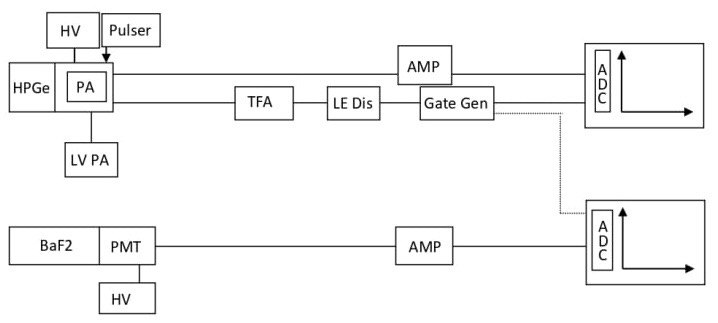
\includegraphics[width=9cm]{catene_elettroniche.jpg}
                \end{figure}

        \subsection*{Formule di interesse}
            \subsubsection*{La sottrazione del fondo}
                Lo spettro gamma di una sorgente può essere rappresentato da un istogramma di conteggi che riporta nell'asse delle ascisse il canale, e si possono osservare dei picchi corrispondenti alle energie con cui i fotoni vengono rivelati dall'apparato sperimentale. Tra questi ultimi, in particolare, non si osservano solo i fotoni dovuti ai decadimenti gamma della sorgente, ma anche una radiazione di fondo e una spalla dovuta all'effetto Compton. A tal proposito, nell'ottica di studiare le sole energie di decadimento, è possibile eseguire una misura di fondo senza interporre alcuna sorgente, quindi sottrarre ai conteggi $CH$ di ciascun bin una quantità opportunamente pesata con il tempo di acquisizione $T$:
                \begin{equation}\label{for:sottrazione_fondo}
                    CH_{eff}=CH_{mis}-\frac{T_{mis}}{T_{fondo}}\cdot CH_{fondo}
                \end{equation}
                Invece, per quanto riguarda il fondo Compton, è possibile eseguire dei fit degli istogrammi corrispondenti alle energie di decadimento non con la sola funzione gaussiana, ma sommando anche un polinomio di primo grado:
                \begin{equation}\label{for:fit_picco}
                    fit(x)=\frac{N}{\sigma\sqrt{2\pi}}e^{\frac{(CH-X)^2}{2\sigma^2}}+A\cdot CH + B
                \end{equation}

                Quando, invece, due picchi successivi non sono ben distinti a causa della scarsa risoluzione, diventa necessario eseguire il fit mediante la somma di due gaussiane, e questo potrebbe essere il caso di un rivelatore a scintillazione per il cobalto-60.

            \subsubsection*{La calibrazione}
                Per poter associare a ciascun canale dell'asse delle ascisse una corrispondente energia, è necessario effettuare una procedura di calibrazione: ci si aspetta che la relazione tra energie e canali sia polinomiale, come nella \eqref{for:fit_calibrazione}.
                \begin{equation}\label{for:fit_calibrazione}
                    E=\sum_{i=0}^{N} \alpha_i(canale)^i
                \end{equation}
                Dove alpiù, per un rivelatore HpGe, ci aspetta di avere un polinomio di primo grado e quindi una calibrazione lineare.
                
            \subsubsection*{La risoluzione e il rumore elettronico}
                Nei rivelatori a semiconduttore è possibile mettere in evidenza come la risoluzione migliori ad alte energie. In particolare, ci si aspetta che l'andamento della risoluzione di ciascun picco in funzione dell'energia tabulata corrispondente abbia l'andamento specifico della formula \eqref{for:fit_risoluzione}:
                \begin{equation}\label{for:fit_risoluzione}
                    R(E)=\sqrt{\frac{a}{E^2}+\frac{b}{E}+c}
                \end{equation}
                Dove:
                \begin{itemize}
                    \item Il termine $a$ quantifica il peggioramento della risoluzione dovuto al rumore elettronico;
                    \item Il termine $b$ quantifica il peggioramento della risoluzione dovuto alle fluttuazioni statistiche per la fisica del principio di funzionamento, ovvero la creazione della coppia elettrone-lacuna;
                    \item Il termine $c$ quantifica il peggioramento della risoluzione dovuto a difetti nella raccolta delle cariche che costituisce il segnale (charge trapping), e può aumentare qualora il rivelatore fosse danneggiato.
                \end{itemize}

                A tal proposito, nel caso particolare in cui il segnale è dato da un pulser che va direttamente al preamplificatore, il secondo e il terzo termine sono nulli perché non vi è nessuna creazione di coppia con conseguente raccolta del segnale, e la sua risoluzione associata è direttamente legata al solo rumore elettronico come nella formula \eqref{for:risoluzione_pulser}:
                \begin{equation}\label{for:risoluzione_pulser}
                    R_{\text{pulser}}=\frac{\sqrt{\Tilde{a}}}{E_{\text{pulser}}}
                \end{equation}

            \subsubsection*{L'attività}
                L'attività è definita come il numero di decadimenti per unità di tempo, e sfruttando la legge del decadimento radioattivo è possibile determinarla al tempo $t$ conoscendo il suo valore al tempo $0$ mediante la formula \eqref{for:attività}:
                \begin{equation}\label{for:attività}
                    A=\left|\frac{dN}{dt}\right|=\left|\frac{d}{dt}\left(N_0e^{-\lambda t}\right)\right|=\lambda N_0e^{-\lambda t}=A_0e^{-\lambda t}
                \end{equation}
                Per cui, conoscendo la costante di decadimento gamma $\lambda$ e l'attività al tempo $0$, è possibile determinare $A$.

            \subsubsection*{Il branching ratio}
                Chiaramente, non tutti i decadimenti della sorgente emettono il fotone che si osserva in un picco, ma solo una parte, che è descritta dal rapporto tra la costante di decadimento parziale della specifica energia e quella totale, detto branching ratio:
                \begin{equation*}
                    B.R.=\frac{\lambda_\text{parziale}}{\lambda_\text{totale}}
                \end{equation*}
                Il suo valore può essere noto in letteratura in corrispondenza di ciascuna energia tabulata.
            
            \subsubsection*{L'efficienza}
                L'apparato sperimentale non è in grado di mettere in evidenza l'emissione di tutti i gamma da parte della sorgente, per almeno due motivi:
                \begin{enumerate}
                    \item La superficie attiva del rivelatore non copre l'intero angolo solido attorno alla sorgente;
                    \item Anche quando la particella incide sulla superficie del rivelatore, non sempre viene rivelata perché potrebbe avvenire durante il tempo morto caratteristico del rivelatore o non produrre gli effetti desiderati.
                \end{enumerate}
                L'insieme di questi due effetti è quantificato mediante l'efficienza assoluta, che è definita come il rapporto tra il numero di particelle rivelate e quello di particelle emesse, e che può essere calcolata mediante la formula \eqref{for:efficienza} per ogni picco dello spettro:
                \begin{equation}\label{for:efficienza}
                    \epsilon=\frac{\text{\# particelle rivelate}}{\text{\# particelle emesse}}=\frac{N}{A\cdot B.R.\cdot T}
                \end{equation}
                Dove:
                \begin{itemize}
                    \item $N$ è il numero di conteggi del picco;
                    \item $A$ è l'attività della sorgente;
                    \item $B.R.$ è il branching ratio specifico della transizione che ha causato l'emissione del fotone a quell'energia;
                    \item $T$ è il tempo vivo di acquizione (live time).
                \end{itemize}
                Di fatto, basta dividere il rate di conteggi misurato per l'attività della sorgente, pesata opportunamente con la branching ratio.

            Sperimentalmente, disponendo di più picchi, ha rilevanza sperimentale studiare l'andamento dell'efficienza assoluta in funzione dell'energia, che nel caso più generale va come:
            \begin{equation*}
                \log{\epsilon}=\sum_{i=0}^{N} \rho_i(\log E)^i
            \end{equation*}
            Dove alpiù, per un rivelatore HpGe, si arresta la sommatoria per $N=2$:
            \begin{equation}\label{for:fit_efficienza}
                \epsilon(E)=\exp[\rho_0+\rho_1\log E+\rho_2(\log E)^2]
            \end{equation}

    \newpage
    \section*{Dati sperimentali}
        Tra i dati, si distinguono:
        \begin{itemize}
            \item Dati noti in letteratura, ovvero energia tabulata di ciascun picco gamma, corrispondente $B.R.$ e costante di decadimento della sorgente;
            \item Dati caratteristici dell'apparato, ovvero attività delle sorgenti impiegate al momento dell'acquisto;
            \item Dati di acquisizione scelti durante la misura, ovvero shaping time, gain, tensioni e parametro di differenziazione nel TFA;
            \item Dati acquisiti mediante l'apparato sperimentale, ovvero spettri in canali in formato di testo che contengono anche i tempi di acquisizione (sia il live time che il dead time).
        \end{itemize}

        Nella tabella \ref{tab:energie_tabulate} sono riportate le energie tabulate per l'europio-152 e il cobalto-60 con le corrispondenti $B.R.$:
        \begin{table}[h!]
            \centering
            \caption{energie tabulate}
            \label{tab:energie_tabulate}
            \subtable[Europio-152]
                {
                    $
                    \begin{array}{cc}
                        \toprule
                        \text{energia (keV)}    &   B.R.(\%)    \\
                        \midrule
                        121.78&28.32\\
                        244.70&7.51\\
                        295.94&0.45\\
                        329.43&0.15\\
                        344.28&22.67\\
                        367.79&0.87\\
                        411.12&2.27\\
                        416.05&0.11\\
                        443.98&3.12\\
                        488.66&0.42\\
                        503.39&0.16\\
                        564.02&0.49\\
                        566.42&0.13\\
                        586.29&0.46\\
                        656.38&0.15\\
                        671.15&0.23\\
                        778.91&12.96\\
                        867.38&4.23\\
                        964.13&14.62\\
                        1085.84&10.11\\
                        1112.07&13.67\\
                        1408.10&20.85\\
                        \bottomrule
                    \end{array}
                    $
                }
            \subtable[Cobalto-60]
                {
                   $
                    \begin{array}{cc}
                        \toprule
                        \text{energia (keV)}    &   B.R.(\%)    \\
                        \midrule
                        1173.20    &   98.85    \\
                        1332.50   &   99.98    \\
                        \bottomrule
                    \end{array}
                    $
                }
        \end{table}

        Nella tabella \ref{tab:attività_costanti_decadimento} sono riportate le costanti di decadimento delle sorgenti impiegate e la loro attività con il momento dell'acquisto:
        \begin{table}[h!]
                \centering
                \caption{attività e costanti di decadimento europio-152 e cobalto-60}
                \label{tab:attività_costanti_decadimento}
                $
                \begin{array}{cccc}
                    \toprule
                    \text{sorgente}       & A_0\:\si{(\kilo\becquerel)}      & \lambda\:\si{(\second^{-1})}  &\text{data acquisto}\\
                    \midrule
                    \text{Europio-152}&37&1.62\cdot10^{-9}&\text{marzo del 2000}\\
                    \text{Cobalto-60}&37&4.17\cdot10^{-9}&\text{giugno del 1998}\\
                    \text{Cobalto-60 (alto rateo)}&430&4.17\cdot10^{-9}&\text{giugno del 1998}\\
                    \bottomrule
                \end{array}
                $
            \end{table}

        \newpage
        Nella tabella \ref{tab:parametri_lavoro} sono riportati i parametri di lavoro per le catene elettroniche dei due rivelatori impiegati:
        \begin{table}[h!]
            \centering
            \caption{parametri di lavoro}
            \label{tab:parametri_lavoro}
            $
            \begin{array}{ccc}
                \toprule
                \text{rivelatore}&\text{HpGe}&\text{BaF}\\
                \midrule
                \text{gain}&\SI{200}{}&\SI{500}{}\\
                \text{shaping time}&\SI{3}{\micro\second}&\SI{3}{\micro\second}\\
                \text{tensione}&\SI{2700}{\volt}&\SI{2100}{\volt}\\
                \text{diff}&200&\text{//}\\
                \bottomrule
            \end{array}
            $
        \end{table}

        Infine, a seguire sono indicati l'elenco delle acquisizioni e quindi i nomi assegnati a ciascun file di testo (il numero non indica l'ordine di acquisizione) e i tempi di acquisizione per ciascuno nella tabella \ref{tab:tempi_acquisizione}.
        \begin{align*}
            &1 \textit{ spettro\_cobalto\_germanio.txt}&&\text{spettro cobalto-60, rivelatore germanio}\\
            &2 \textit{ spettro\_cobalto\_germanio\_monopicco.txt}&&\text{spettro cobalto-60, rivelatore germanio (soglia)}\\
            &3 \textit{ spettro\_cobalto\_germanio\_highrate.txt}&&\text{spettro cobalto-60 alto rateo, rivelatore germanio}\\
            &4 \textit{ spettro\_fondo\_germanio.txt}&&\text{spettro fondo, rivelatore germanio}\\
            &5 \textit{ spettro\_pulser\_germanio.txt}&&\text{spettro con pulser, rivelatore germanio}\\
            &6 \textit{ spettro\_incognita\_germanio.txt}&&\text{spettro sorgente incognita, rivelatore germanio}\\
            &7 \textit{ spettro\_europio\_germanio.txt}&&\text{spettro europio-152, rivelatore germanio}\\
            &8 \textit{ spettro\_cobalto\_baf.txt}&&\text{spettro cobalto-60, rivelatore fluoruro di bario}\\
            &9 \textit{ spettro\_cobalto\_baf\_monopicco.txt}&&\text{spettro cobalto-60, rivelatore fluoruro di bario (soglia)}\\
        \end{align*}

        \begin{table}[h!]
                \centering
                \caption{Tempi di acquisizione}
                \label{tab:tempi_acquisizione}
                $
                \begin{array}{ccc}
                    \toprule
                    \text{\#acquisizione}&\text{Live-time (\si{\second})}&\text{Dead-time (\si{\second})}\\
                    \midrule
                    1&301&310\\
                    2&429&441\\
                    3&8499&8617\\
                    4&8315&8378\\
                    5&671&674\\
                    6&53745&54212\\
                    7&341&383\\
                    8&421&429\\
                    9&589&627\\
                    \bottomrule
                \end{array}
                $
            \end{table}

    \newpage
    \section{La calibrazione in energia del rivelatore al germanio}
        Il software dell'apparato sperimentale fornisce uno spettro in canali, e nota la sorgente gamma è possibile effettuare una calibrazione in energia sfruttando i valori noti in letteratura di quelle con cui le particelle gamma vengono emesse, tenendo conto della loro intensità percentuale, riportate nella tabella \ref{tab:energie_tabulate}.

        Il fatto che la relazione tra canali ed energie tabulate sia effettivamente lineare non è un fatto scontato. Infatti, in generale, nei rivelatori HpGe, la funzione polinomiale di fit può arrivare anche al grado 5. A tal proposito, l'unico modo per capire a quale grado arrestarsi è vedere l'andamento dei residui: se con il fit di grado n essi seguono un qualche andamento (per esempio crescente), è conveniente aumentare il grado a n+1, fino a quando l'andamento non è casuale.

        Complessivamente, per questa fase dell'analisi dati, è possibile sfruttare dei codici che sono in grado di leggere i dati dei file di testo, salvare i plot degli spettri e dei singoli picchi, calcolare i parametri dei fit gaussiani ed eseguire il best fit polinomiale per la calibrazione.
                
        \subsection*{Il funzionamento dei codici}
            Questa procedura di analisi dati ha richiesto l'utilizzo di tre codici:
            \begin{itemize}
                \item La macro \textit{spettro.cpp} è in grado di leggere i dati nei file di testo forniti dall'apparato sperimentale, salvare i plot dello spettro e dei singoli picchi e fare di questi ultimi il fit, come nella \eqref{for:fit_picco}.
                
                \textbf{Input}: spettro in canali della sorgente e parametri di fit in file di testo.
                
                \textbf{Output}: plot spettro in canali e singoli picchi con fit in file pdf, parametri di fit gaussiani in file di testo.
                
                \item La macro \textit{sottrazione\_fondo.cpp} è in grado di leggere i dati nei file di testo forniti dall'apparato sperimentale e sottrarne il fondo, così da modificare il file di input della precedente.
                
                \textbf{Input}: spettro in canali della sorgente e del fondo in file di testo.
                
                \textbf{Output}: spettro in canali della sorgente col fondo sottratto in file di testo.
                
                \item La macro \textit{calibrazione.cpp} è in grado di eseguire il best fit polinomiale di grado $N$ e di calcolare i residui al variare dell'energia dei picchi.
                
                \textbf{Input}: canali con corrispondente incertezza trovati nel primo codice ed energie tabulate in un file di testo.
                
                \textbf{Output}: parametri di fit polinomiale in un file di testo.
            \end{itemize}
            
            \subsubsection*{Note operative}
                La macro \textit{spettro.cpp} non può essere utilizzata subito nella sua interezza, perché è essenziale aiutare la procedura di fit dei singoli picchi gaussiani mediante il comando \textit{SetParameter()}, impostando il centroide e la deviazione standard grossolani per essere sicuri che il codice converga ai valori auspicati. Inoltre, a priori, non si conosce la posizione dei picchi visibili e i loro estremi. A tal proposito, è importante far girare il codice prima commentando le righe che riguardano i fit gaussiani, così da vedere tutti i parametri da inserire nel file di input.

                Inoltre, a priori, non si sa quali energie tabulate per l'europio-152 verrano individuate nello spettro, dato che in letteratura, nella tabella \ref{tab:energie_tabulate}, sono indicati numerosi picchi. Per cui, prima di eseguire la calibrazione definitiva, è conveniente calcolare manualmente una calibrazione provvisoria usando i picchi dell'europio-152 evidentemente corrispondenti, che verosimilmente sono quelli a $B.R.$ più alto, quindi sfruttare i coefficienti trovati per avere indicazioni sulle altre energie auspicabilmente osservate, noti i centroidi:
                \begin{equation}\label{for:fit_calibrazione_provvisoria}
                    \alpha_0=\frac{\Delta E_{tab}}{\Delta X}\qquad\beta_0=E_{tab}-\alpha_0X\qquad E_0=\alpha_0X+\beta_0
                \end{equation}
                Dove le $E_{tab}$ sono le energie tabulate per l'europio-152 a $B.R$ più alto, corrispondenti ai picchi 1 e 3, ed $E_0$ sono tutte le energie provvisorie da confrontare con la tabella \ref{tab:energie_tabulate}.

        \subsection*{La propagazione delle incertezze}
            \subsubsection*{I fit dei picchi}
                Mediante il comando \textit{GetParError()}, i codici forniscono già le incertezze sul numero di conteggi $N$, sul centroide $X$, sulla deviazione standard $\sigma$ per ciascuna gaussiana, e anche su tutti i parametri del fit polinomiale, per cui bisogna calcolare solamente le incertezze sulle quantità calcolate, ovvero la $FWHM$, data da:
                    \begin{equation*}\label{for:numero_conteggi}
                        FWHM=2\sqrt{2\log2}\cdot\sigma\qquad\Rightarrow\qquad2\sqrt{2\log2}\cdot\delta\sigma
                    \end{equation*}

                Di fatto, è ragionevole utilizzare l'errore $\delta X$ sul centroide solamente per la procedura di fit per la calibrazione, per la conversione in energia e i successivi confronti, invece, ha più significato considerare il valore medio entro una $FWHM$.

        \subsection*{I risultati ottenuti}
            La figura \ref{fig:spettri_europio_cobalto_germanio} mostra gli spettri per l'europio-152 e per il cobalto-60 (anche per la sorgente ad alto rateo) con e senza il fondo, mentre le figure \ref{fig:fit_picchi_europio_germanio} e \ref{fig:fit_picchi_cobalto_germanio} mostrano i fit dei singoli picchi.
            
            \begin{figure}[h!]
                \centering
                \caption{spettri in canali}
                \label{fig:spettri_europio_cobalto_germanio}
                \subfigure[europio-152 con fondo\label{fig:spettro_europio_germanio_con_fondo}]
                    {
                        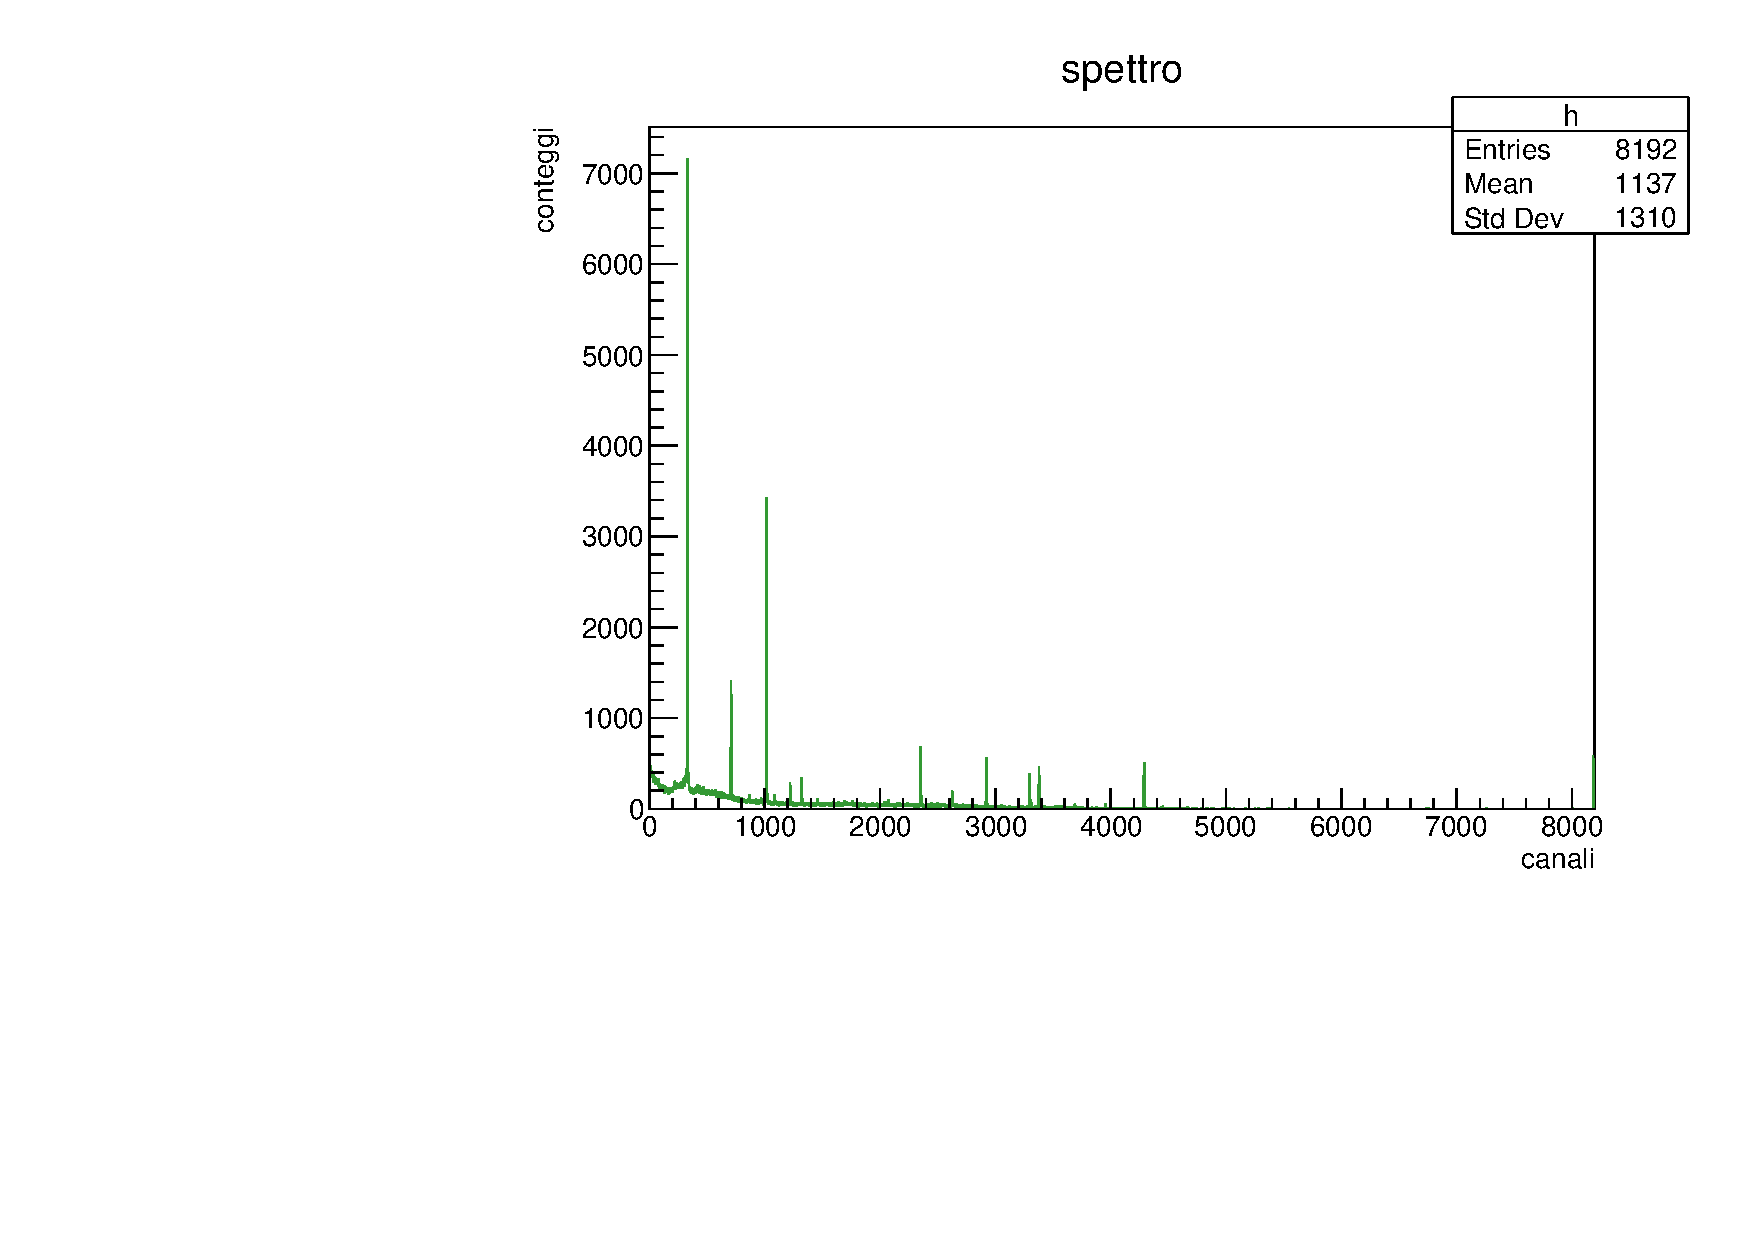
\includegraphics[width=5cm]{grafici/spettro_europio_germanio_con_fondo.pdf}
                    }
                \subfigure[europio-152 senza fondo\label{fig:spettro_europio_germanio_senza_fondo}]
                    {
                        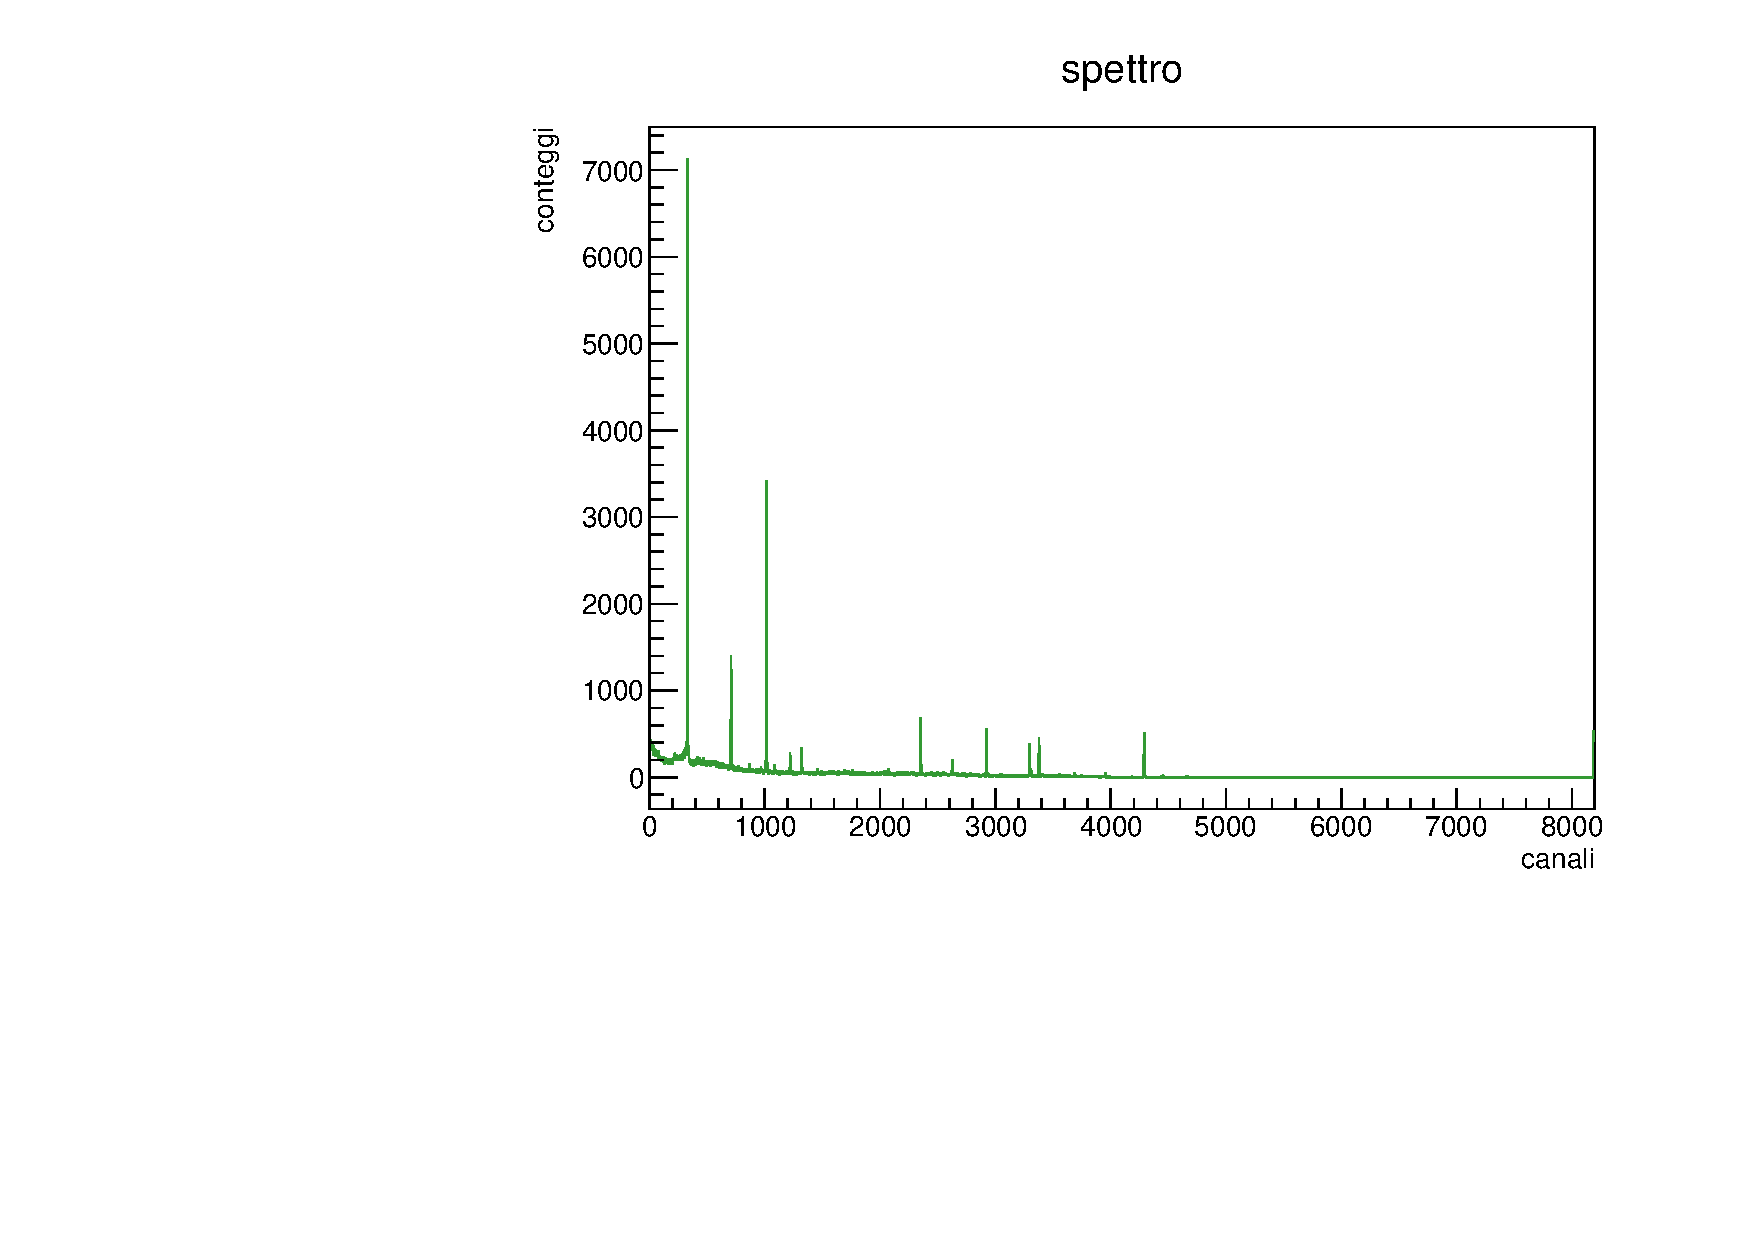
\includegraphics[width=5cm]{grafici/spettro_europio_germanio_senza_fondo.pdf}
                    }
                
                \subfigure[cobalto-60 con fondo\label{fig:spettro_cobalto_germanio_con_fondo}]
                    {
                        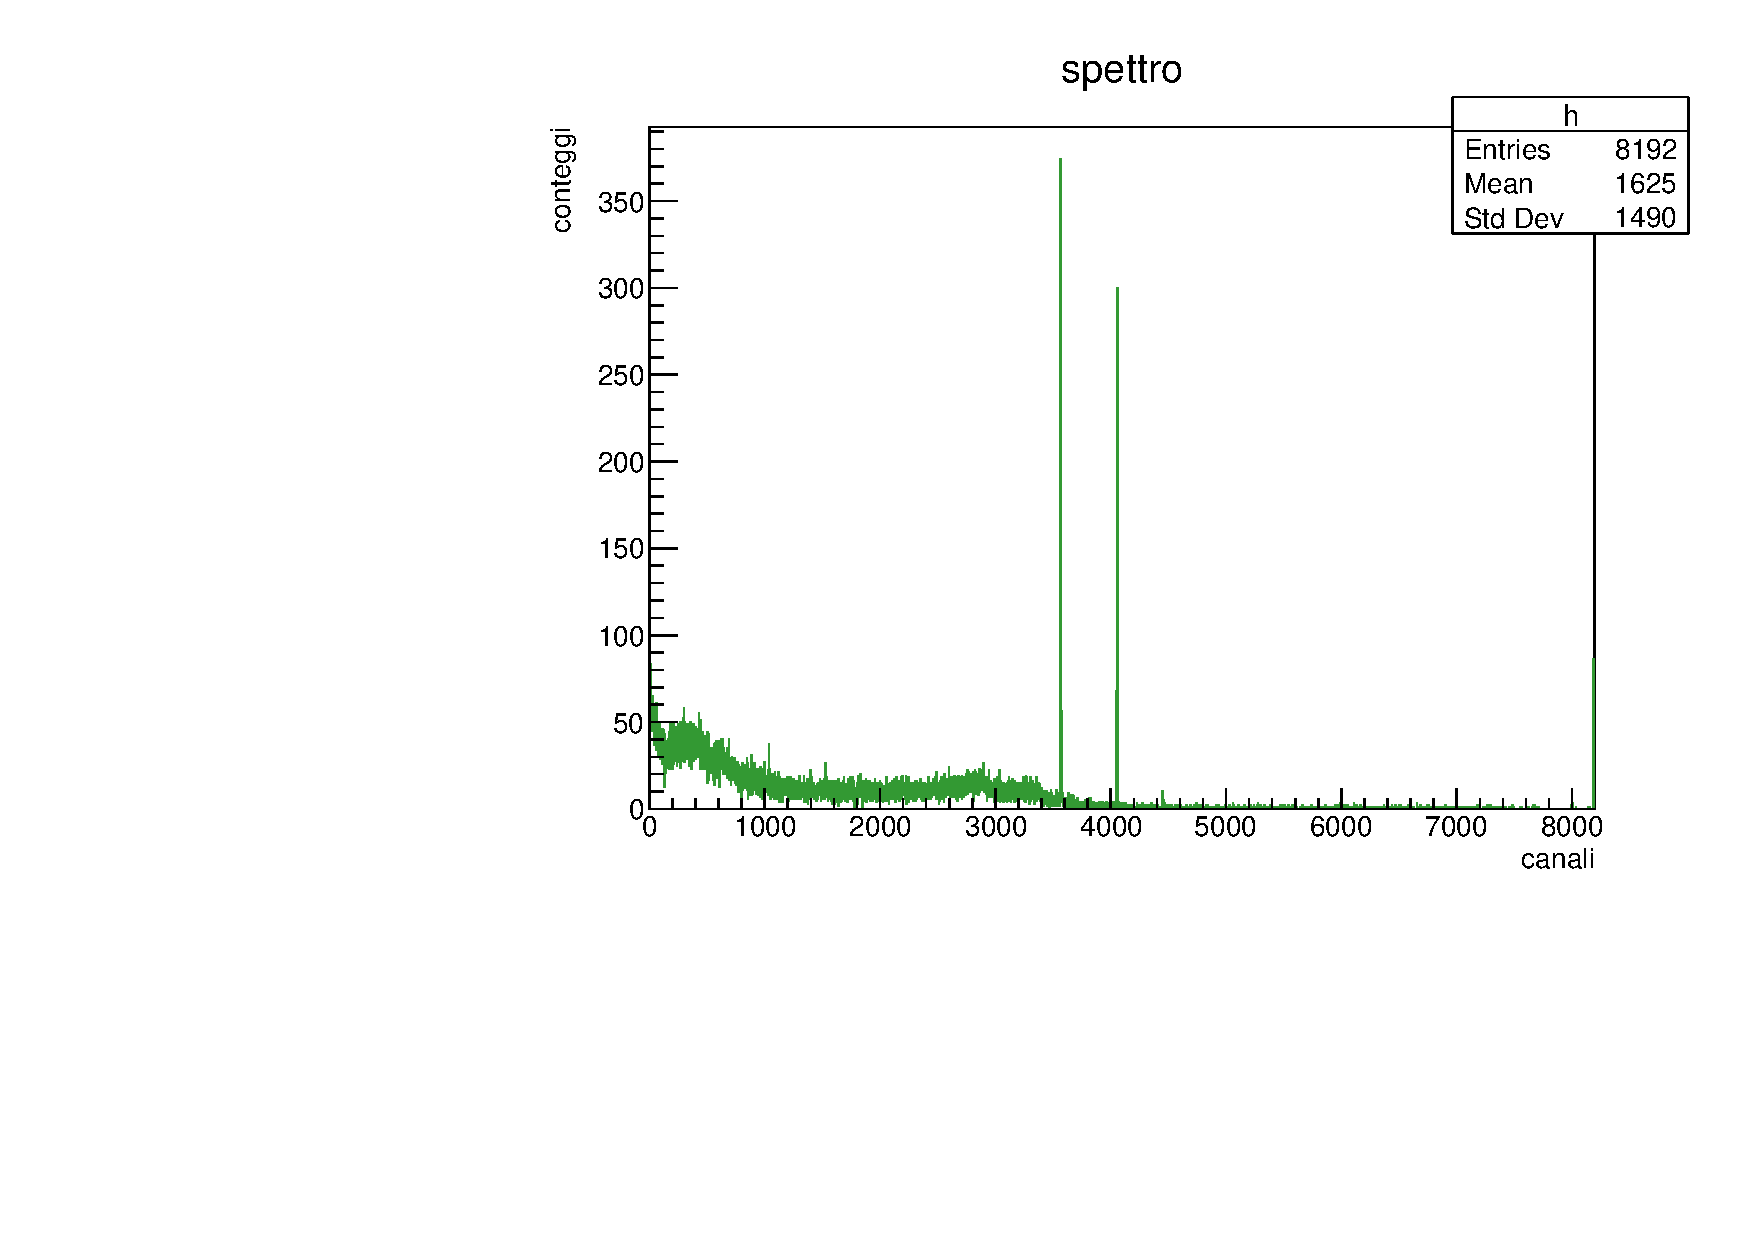
\includegraphics[width=5cm]{grafici/spettro_cobalto_germanio_con_fondo.pdf}
                    }
                \subfigure[cobalto-60 senza fondo\label{fig:spettro_cobalto_germanio_senza_fondo}]
                    {
                        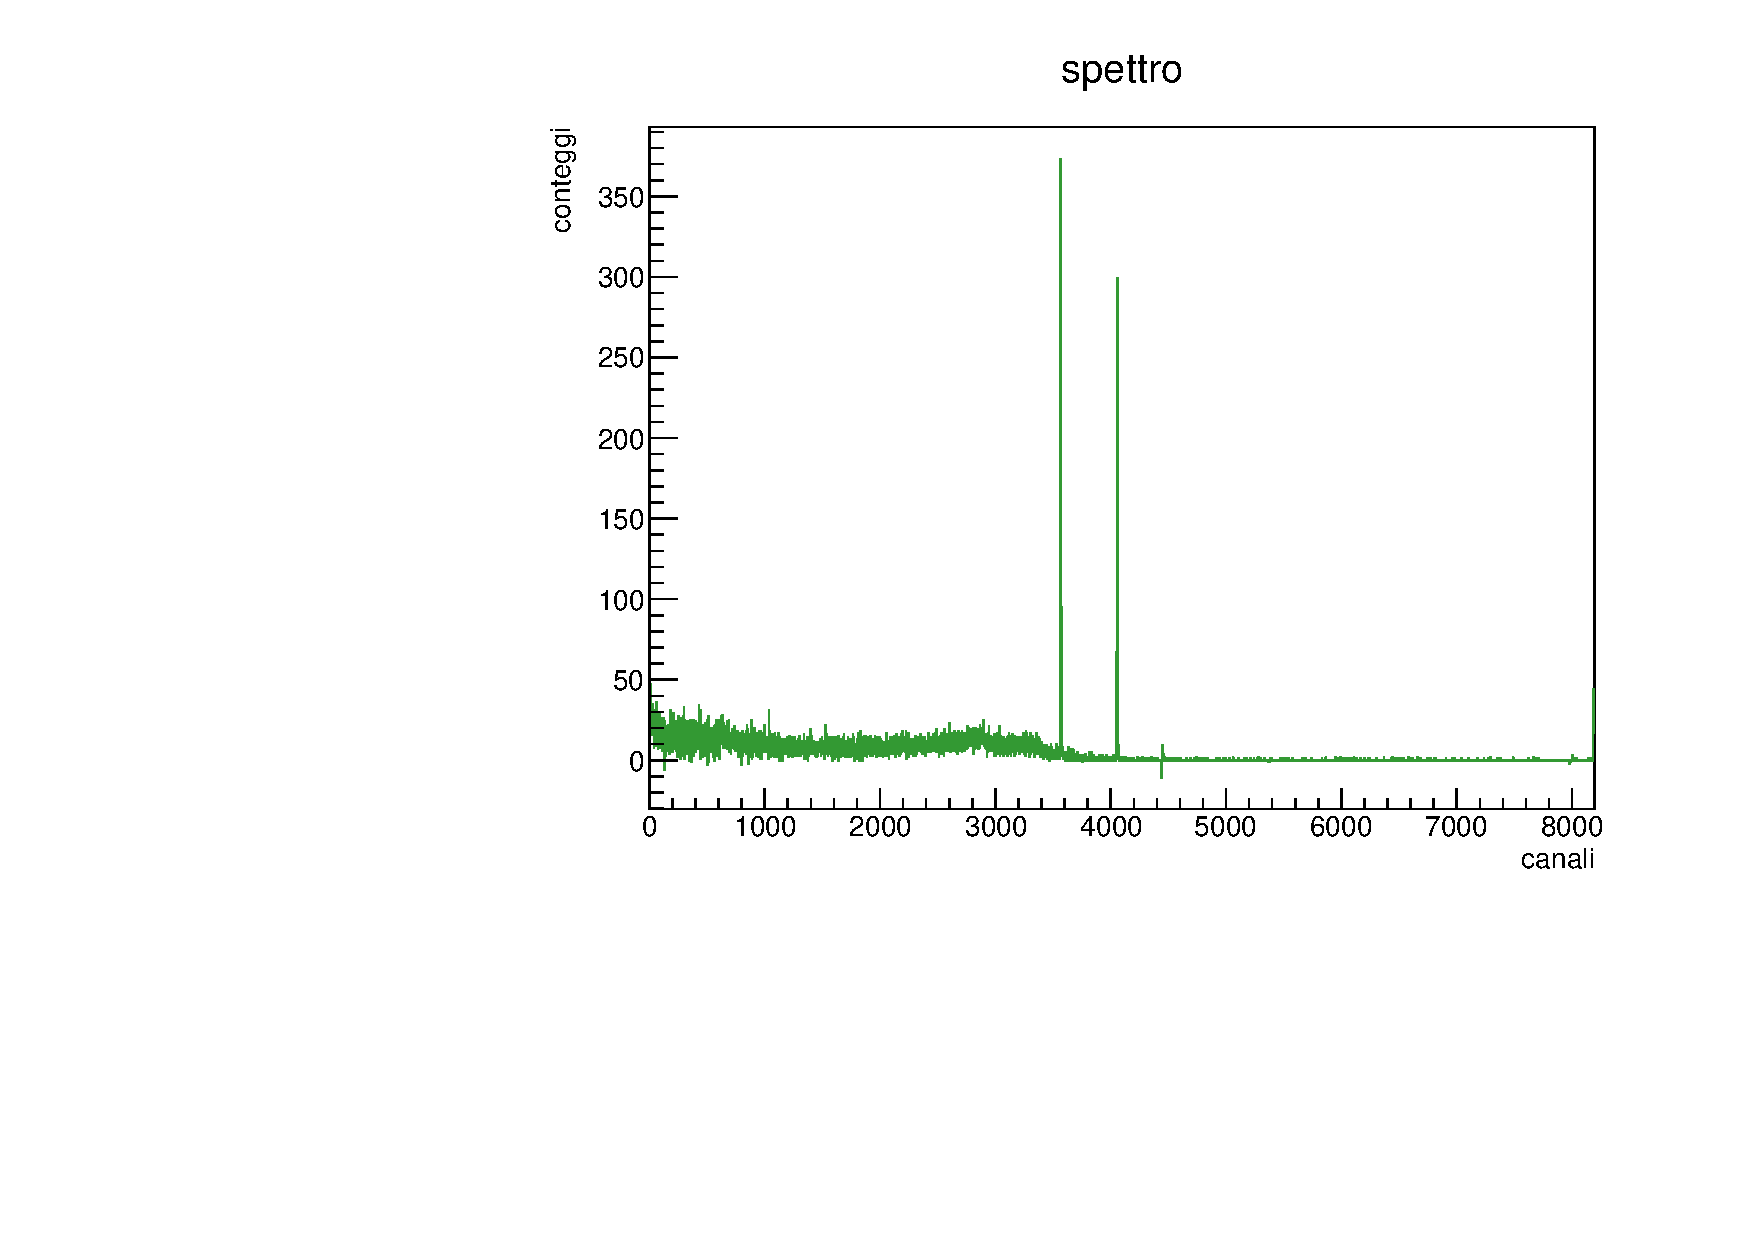
\includegraphics[width=5cm]{grafici/spettro_cobalto_germanio_senza_fondo.pdf}
                    }

                \subfigure[cobalto-60 (alto rateo) con fondo\label{fig:spettro_cobalto_germanio_highrate_con_fondo}]
                    {
                        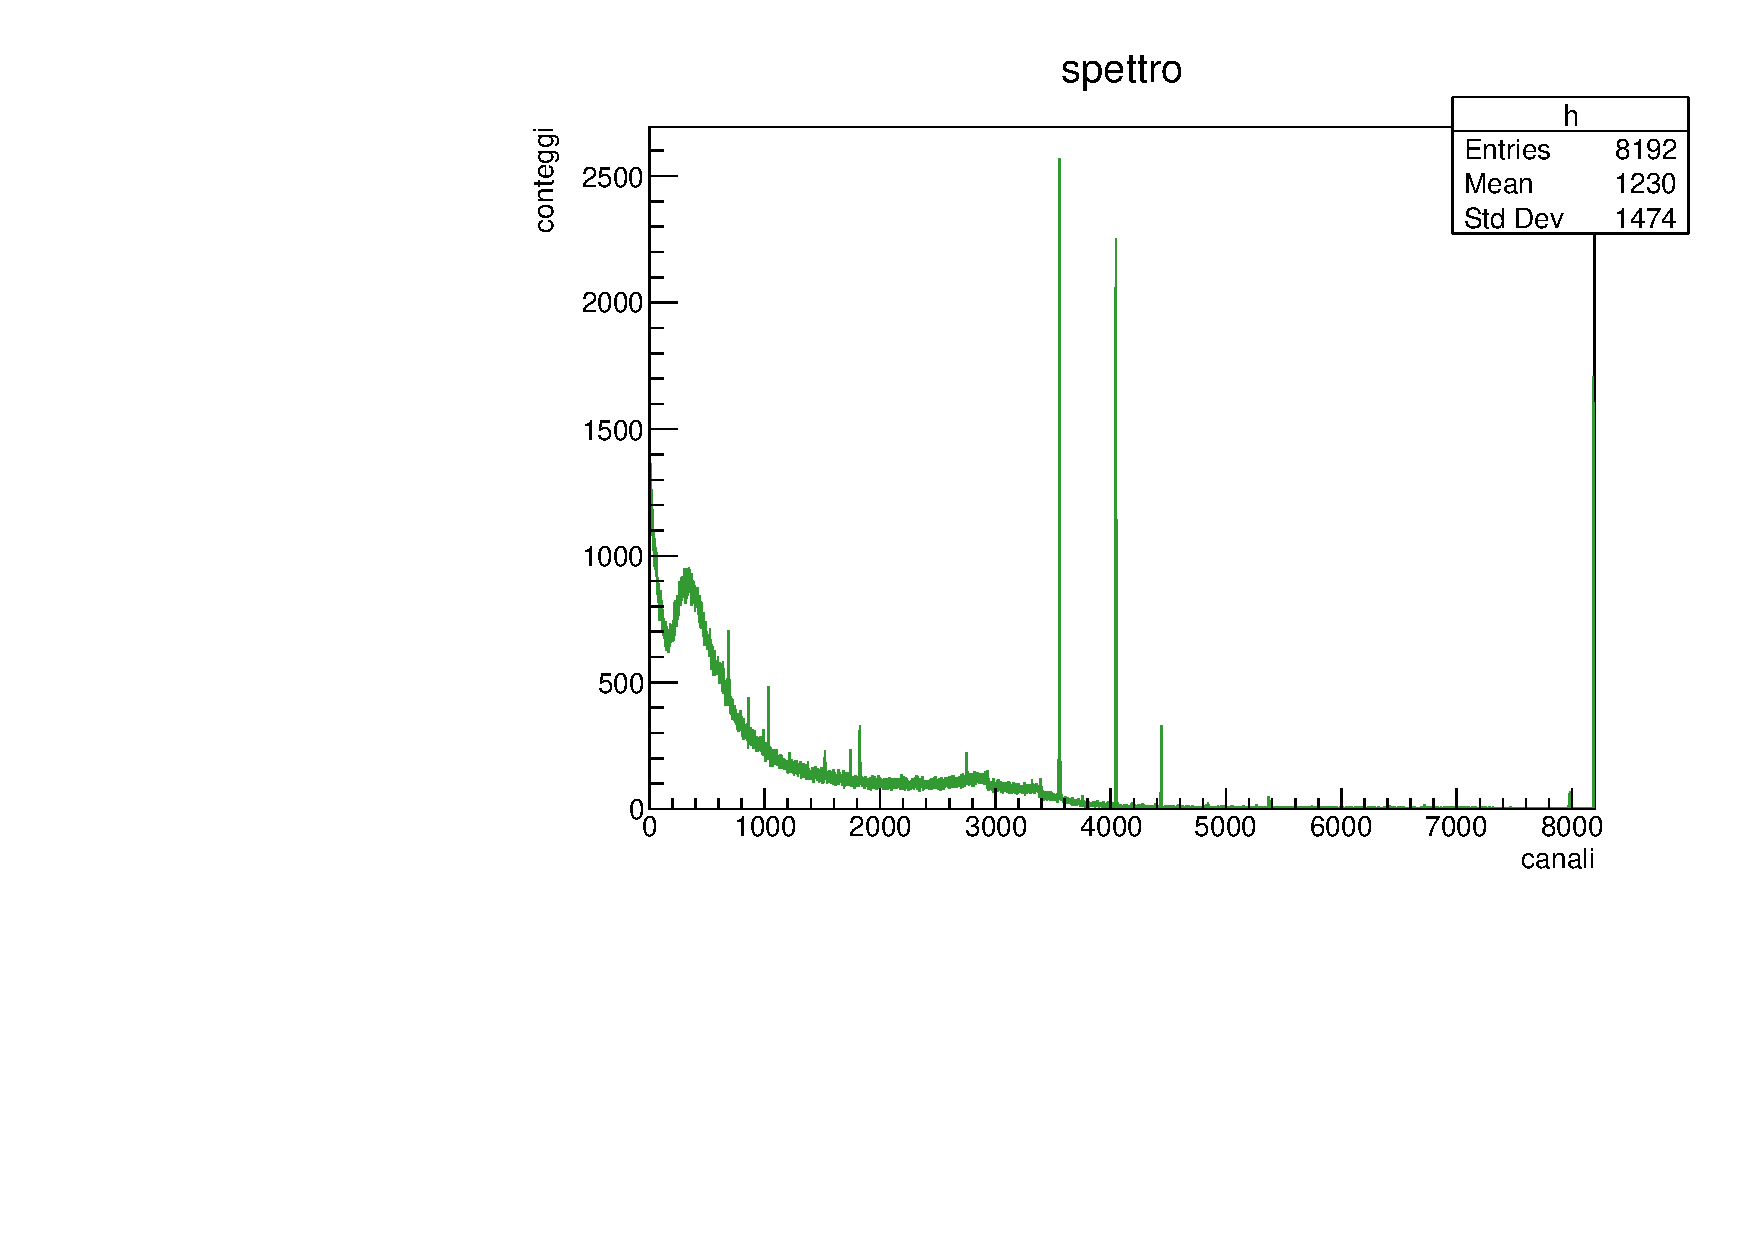
\includegraphics[width=5cm]{grafici/spettro_cobalto_germanio_highrate_con_fondo.pdf}
                    }
                \subfigure[cobalto-60 (alto rateo) senza fondo\label{fig:spettro_cobalto_germanio_highrate_senza_fondo}]
                    {
                        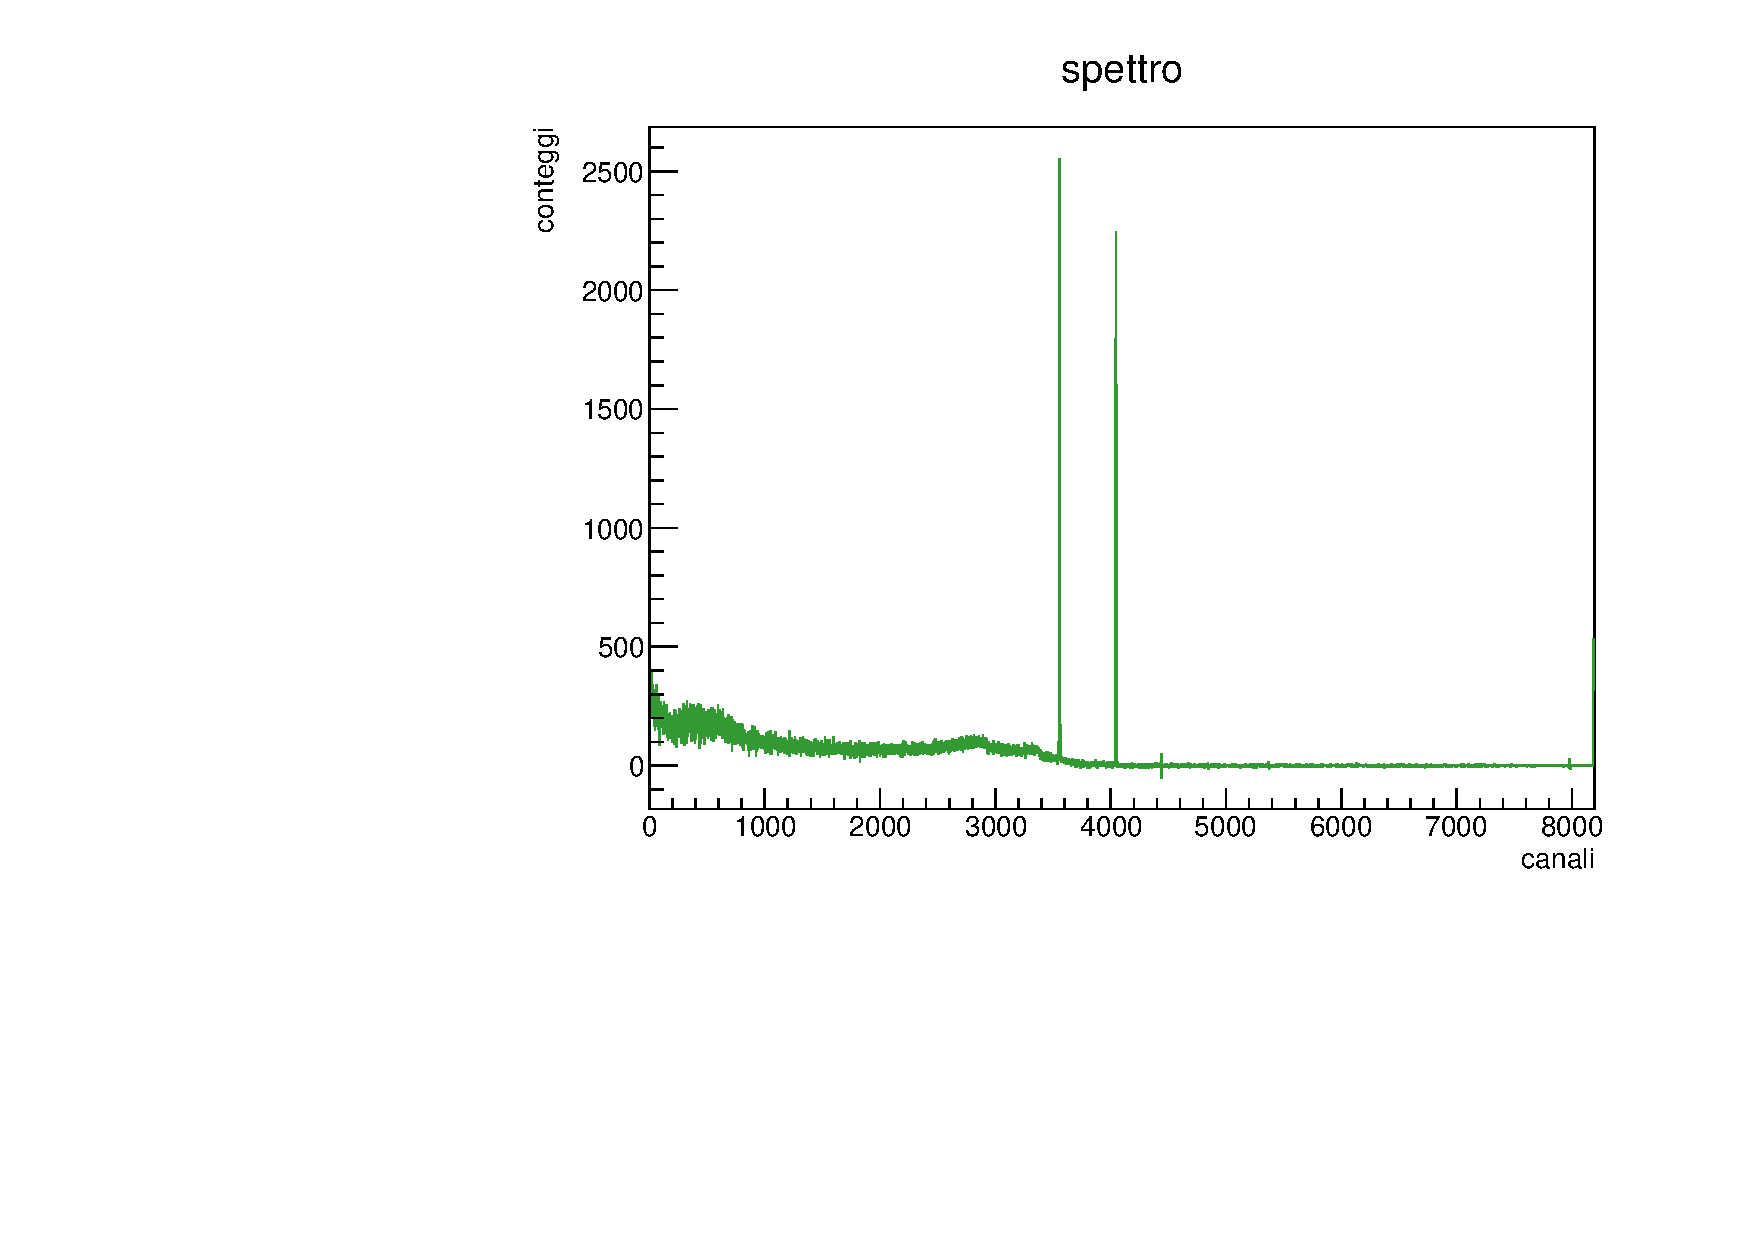
\includegraphics[width=5cm]{grafici/spettro_cobalto_germanio_highrate_senza_fondo.pdf}
                    }
            \end{figure}
            
            \begin{figure}[h!]
                \centering
                \caption{picchi europio-152 con fit}
                \label{fig:fit_picchi_europio_germanio}
                \subfigure[picco 1]
                    {
                        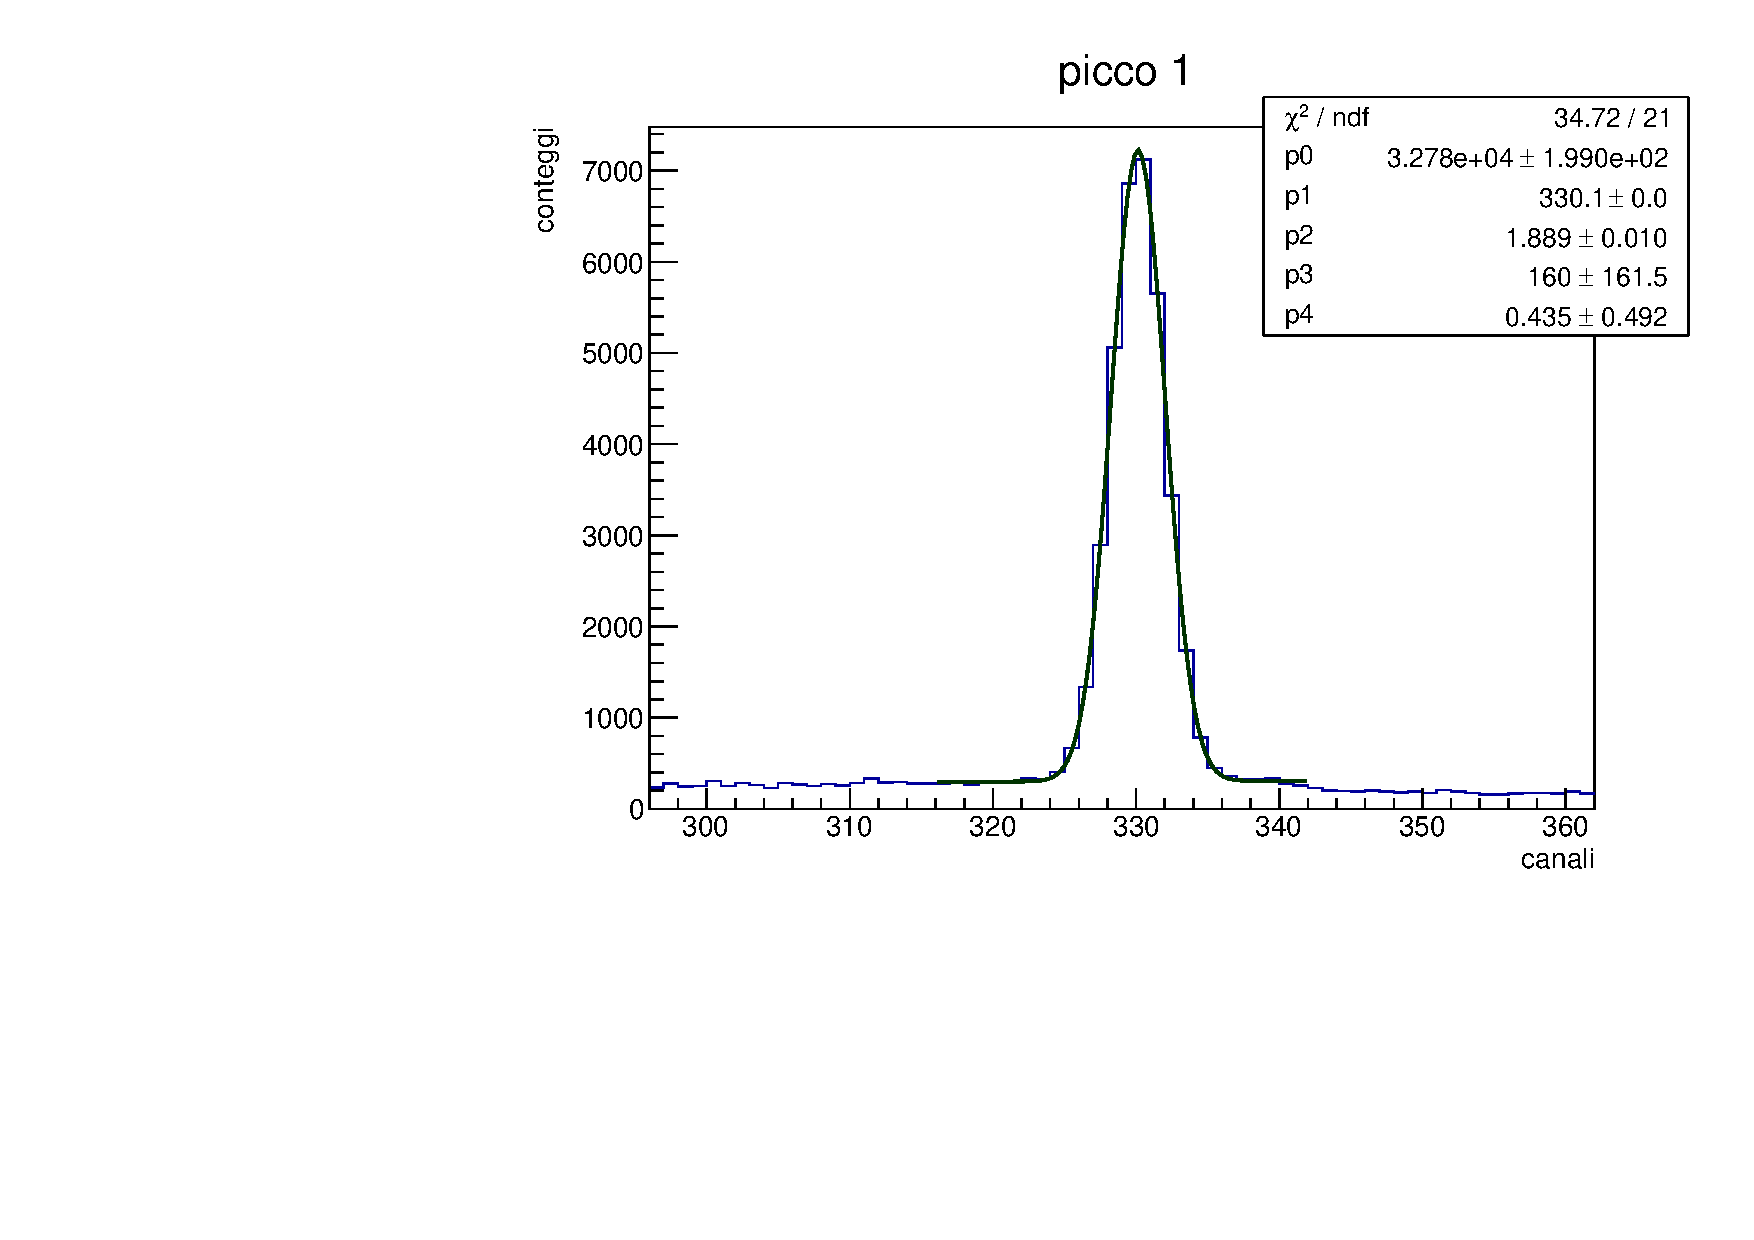
\includegraphics[width=3.4cm]{grafici/picco_europio_germanio_1.pdf}
                    }
                \subfigure[picco 2]
                    {
                        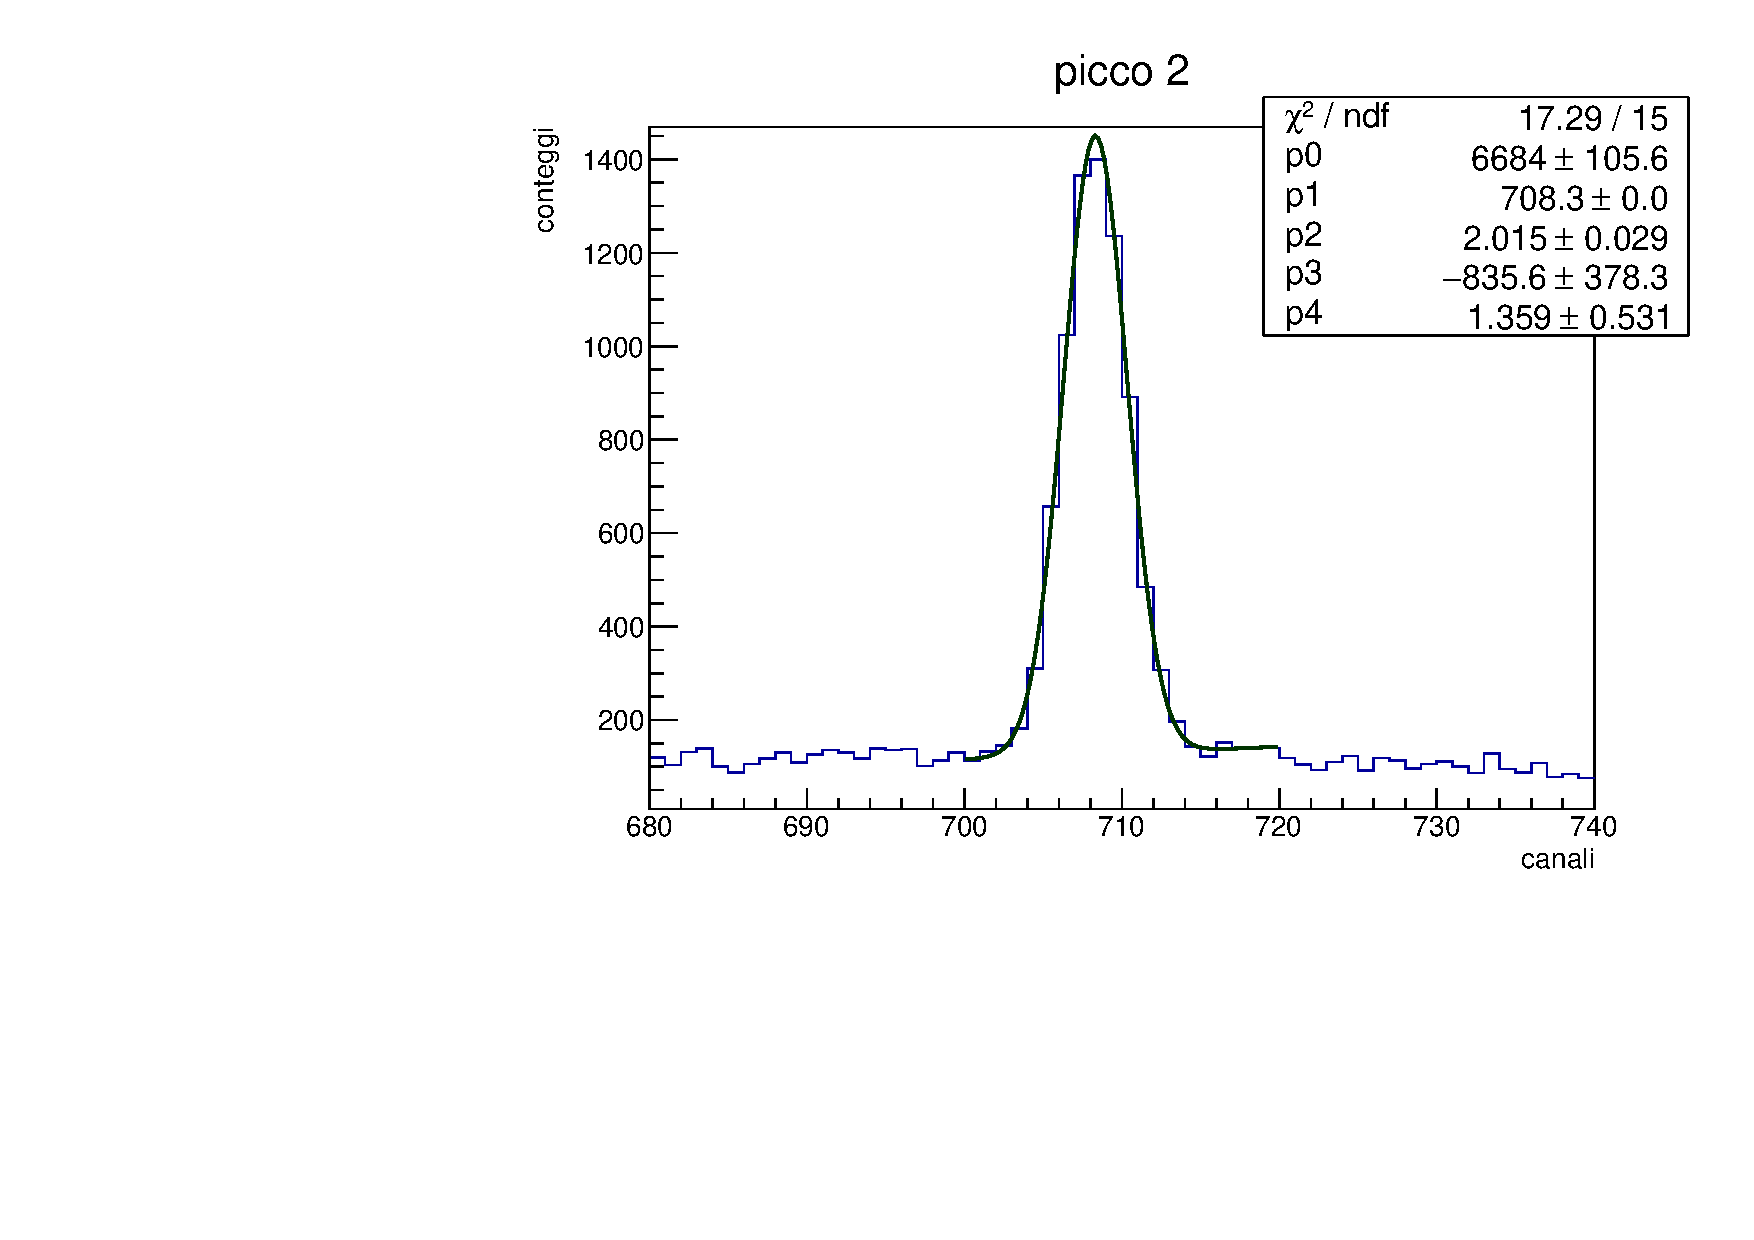
\includegraphics[width=3.4cm]{grafici/picco_europio_germanio_2.pdf}
                    }
                \subfigure[picco 3]
                    {
                        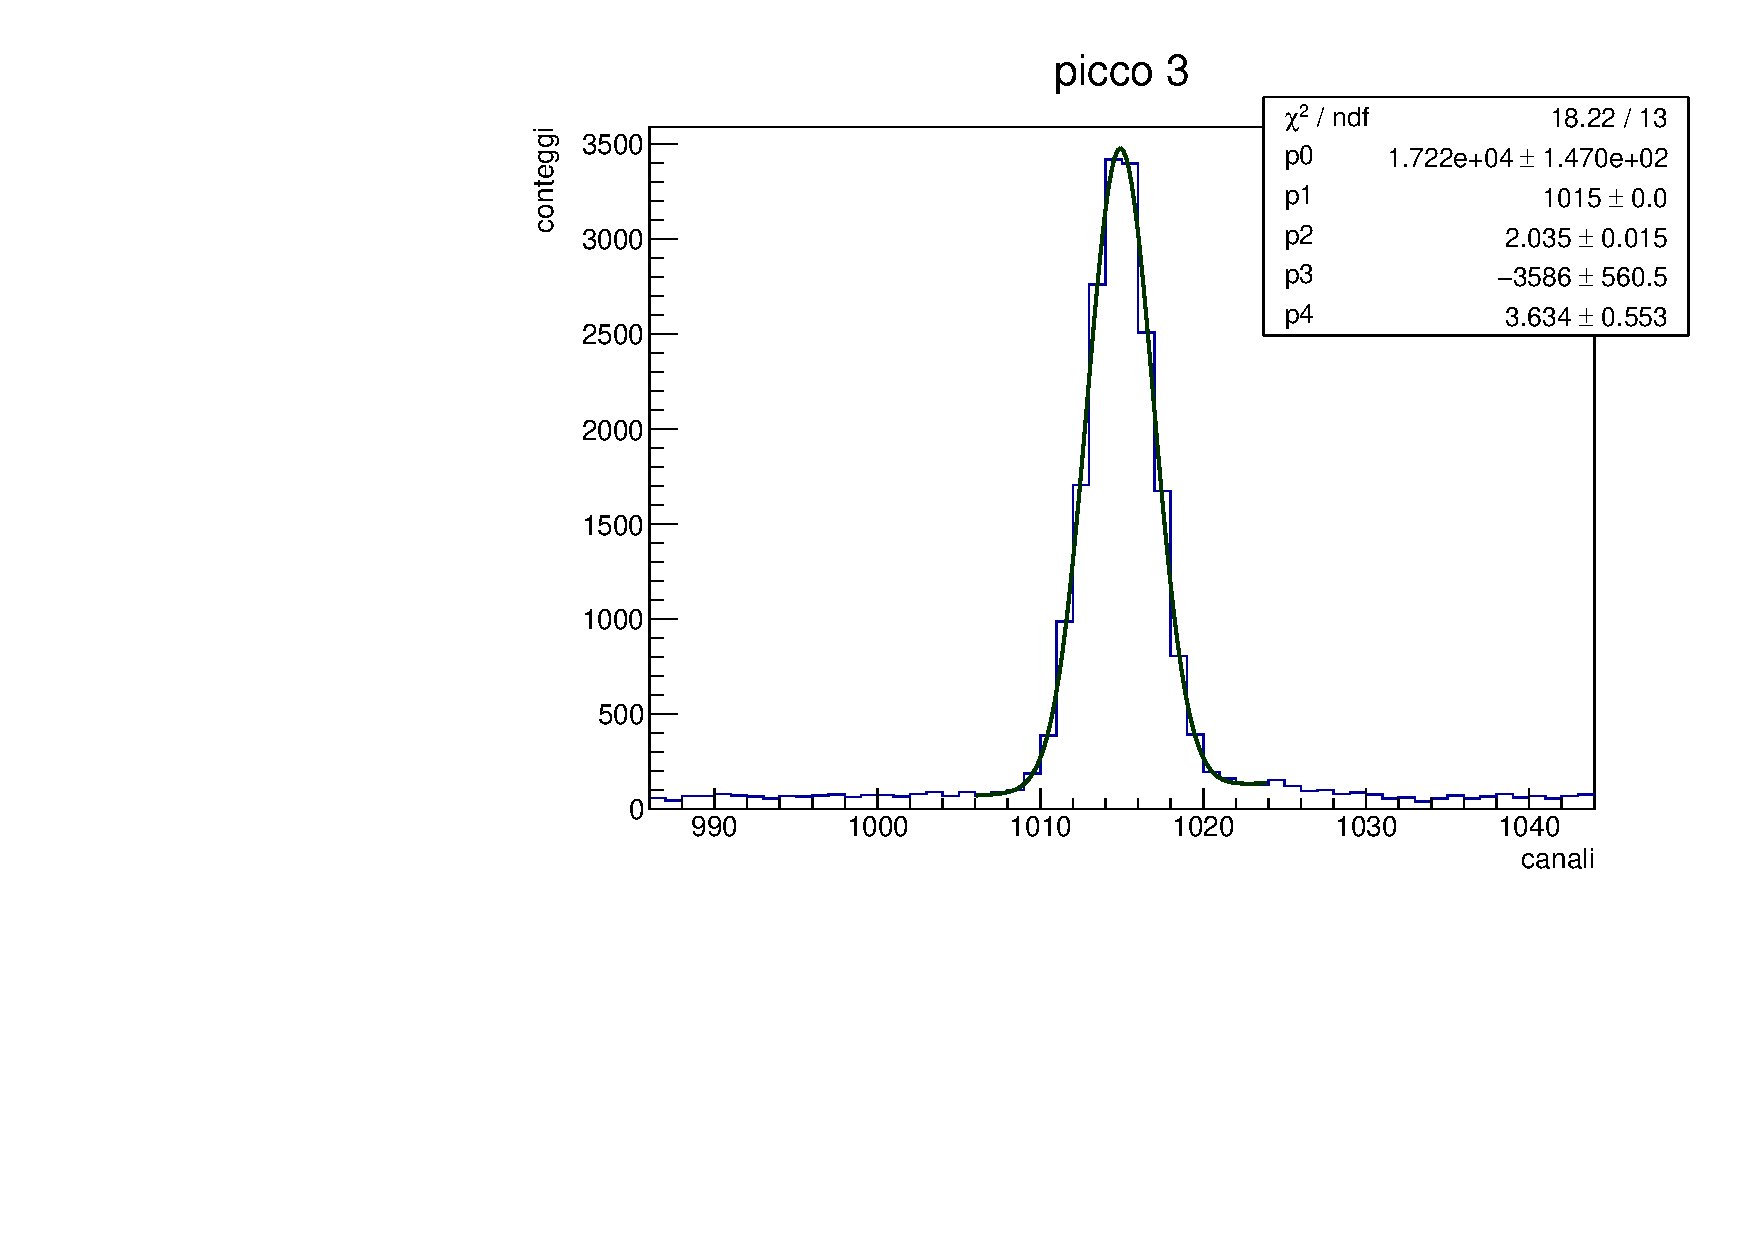
\includegraphics[width=3.4cm]{grafici/picco_europio_germanio_3.pdf}
                    }
                \subfigure[picco 4]
                    {
                        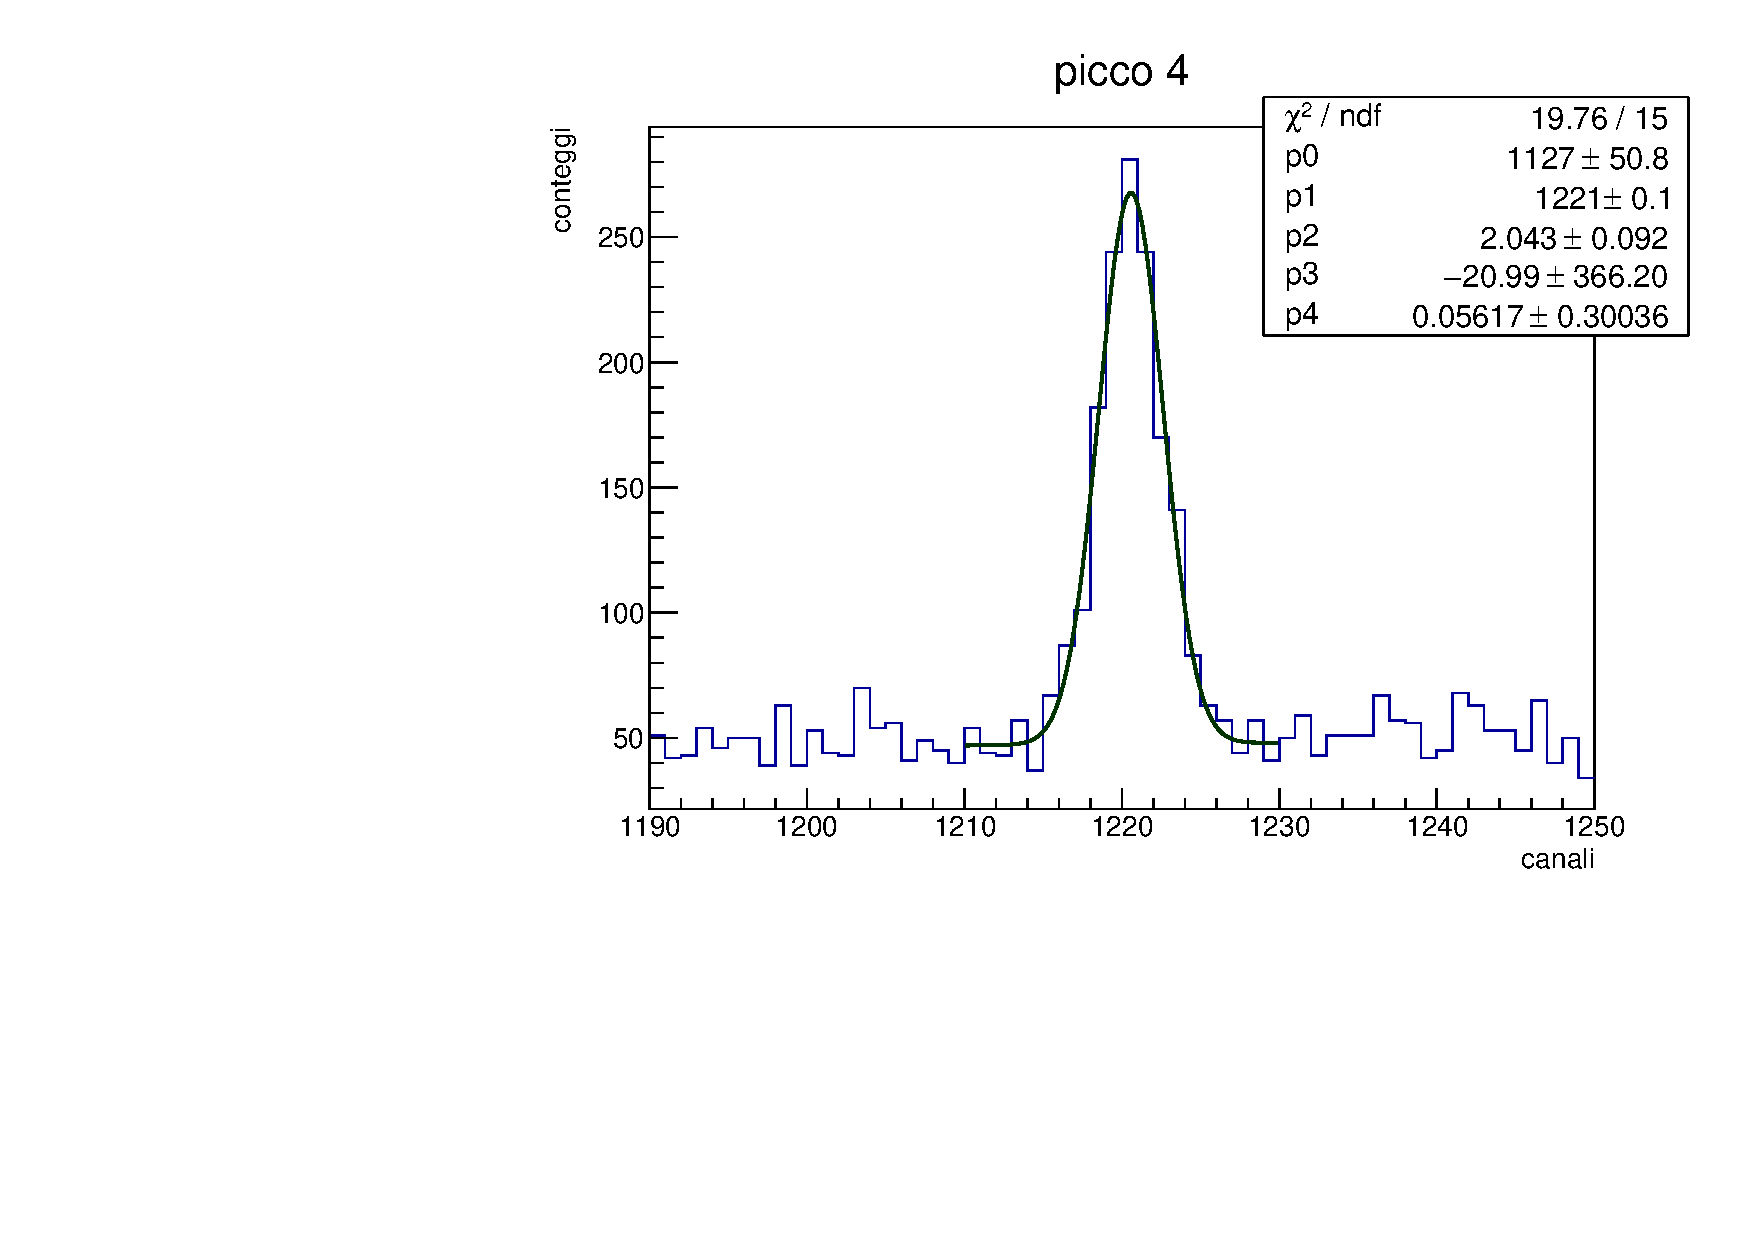
\includegraphics[width=3.4cm]{grafici/picco_europio_germanio_4.pdf}
                    }
                \subfigure[picco 5]
                    {
                        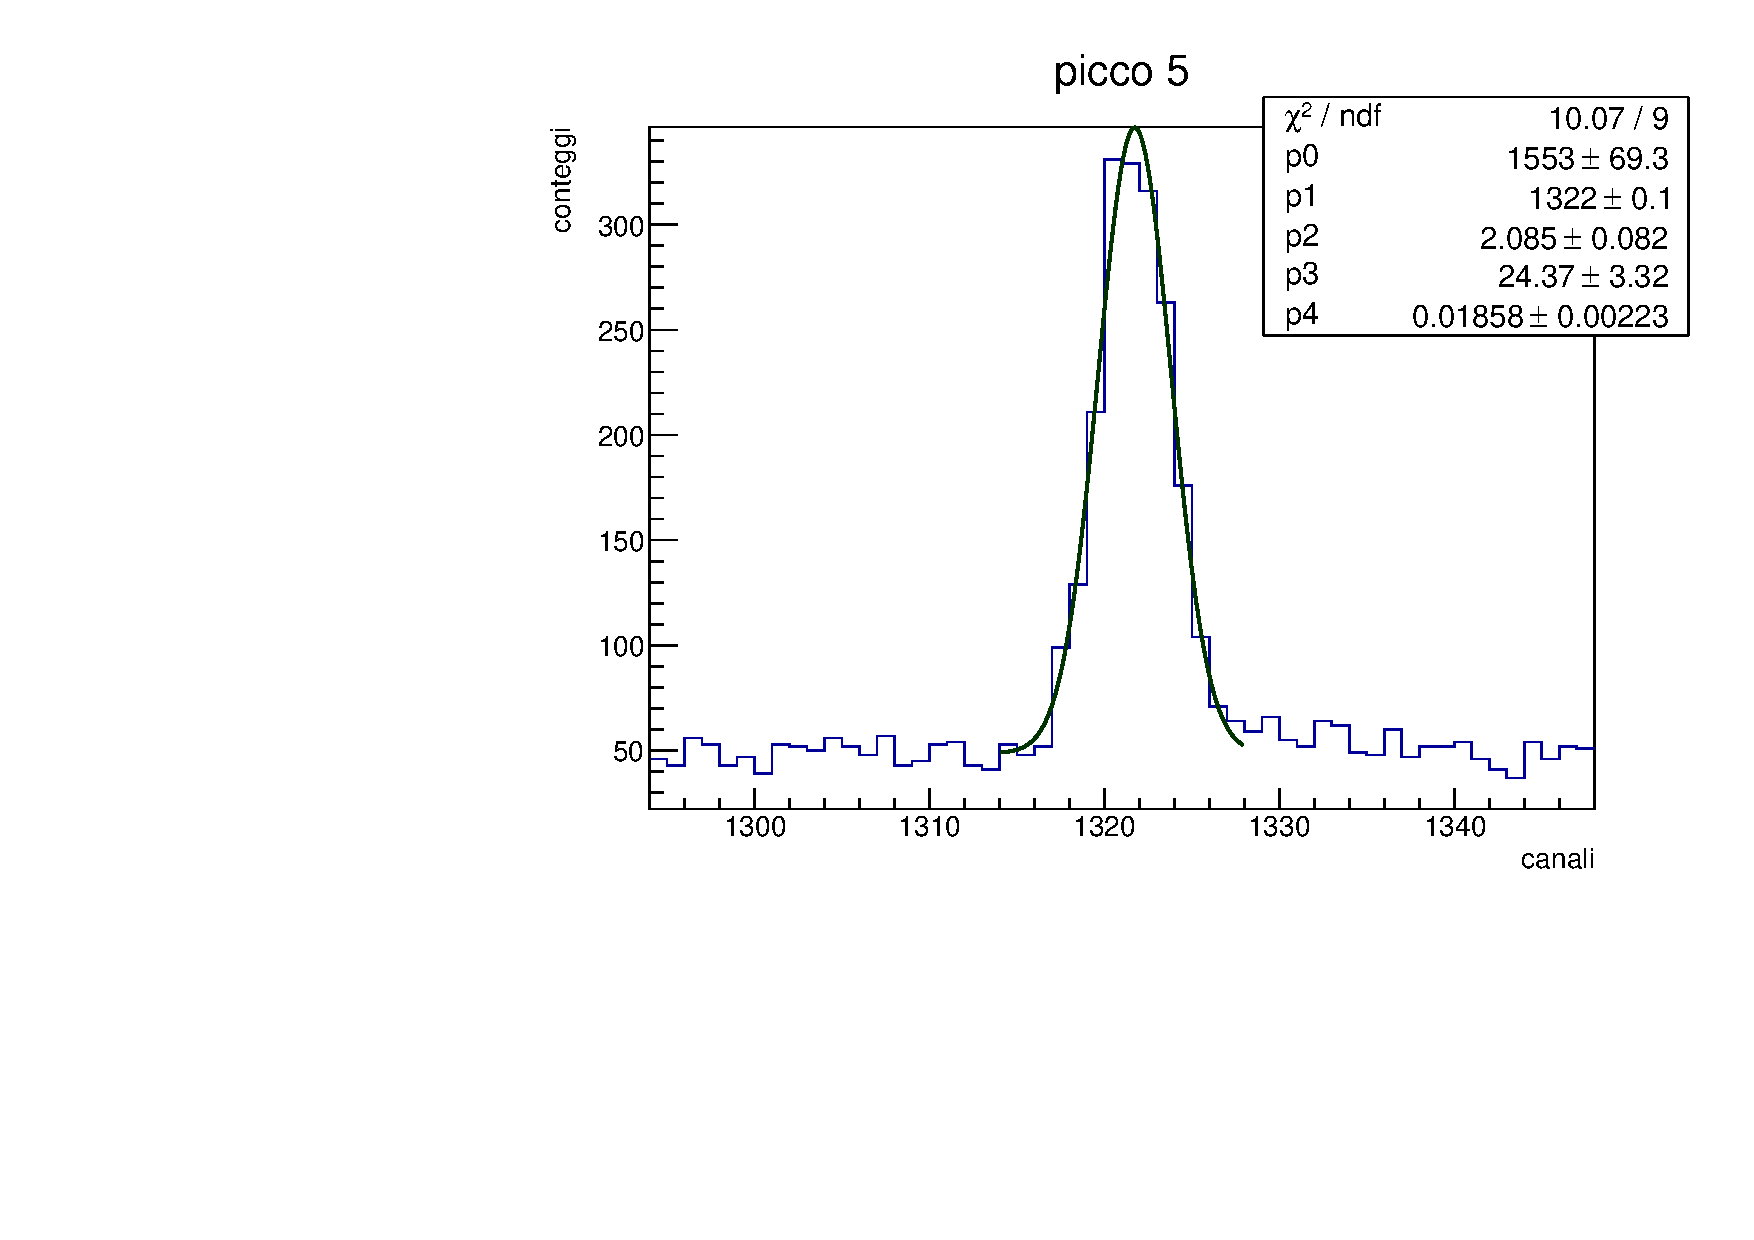
\includegraphics[width=3.4cm]{grafici/picco_europio_germanio_5.pdf}
                    }
                \subfigure[picco 6]
                    {
                        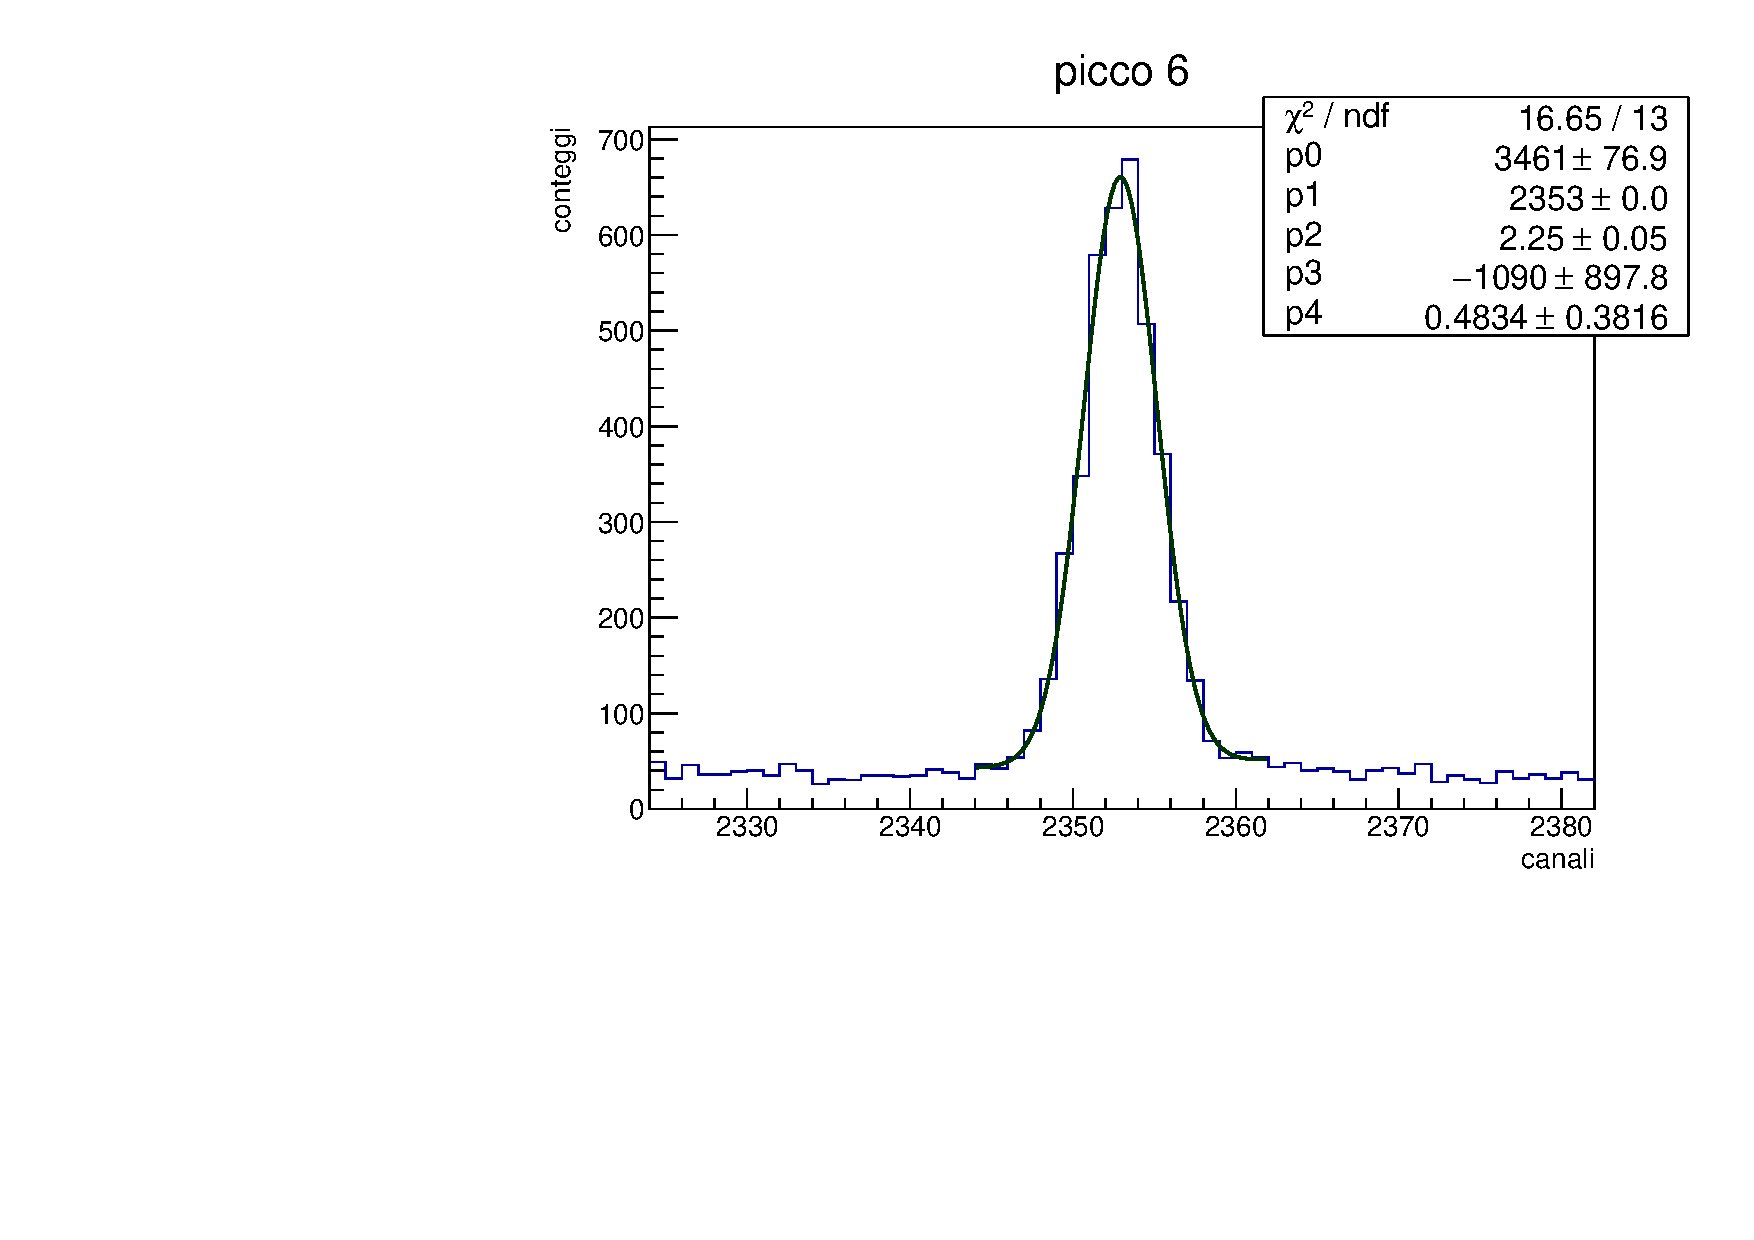
\includegraphics[width=3.4cm]{grafici/picco_europio_germanio_6.pdf}
                    }
                \subfigure[picco 7]
                    {
                        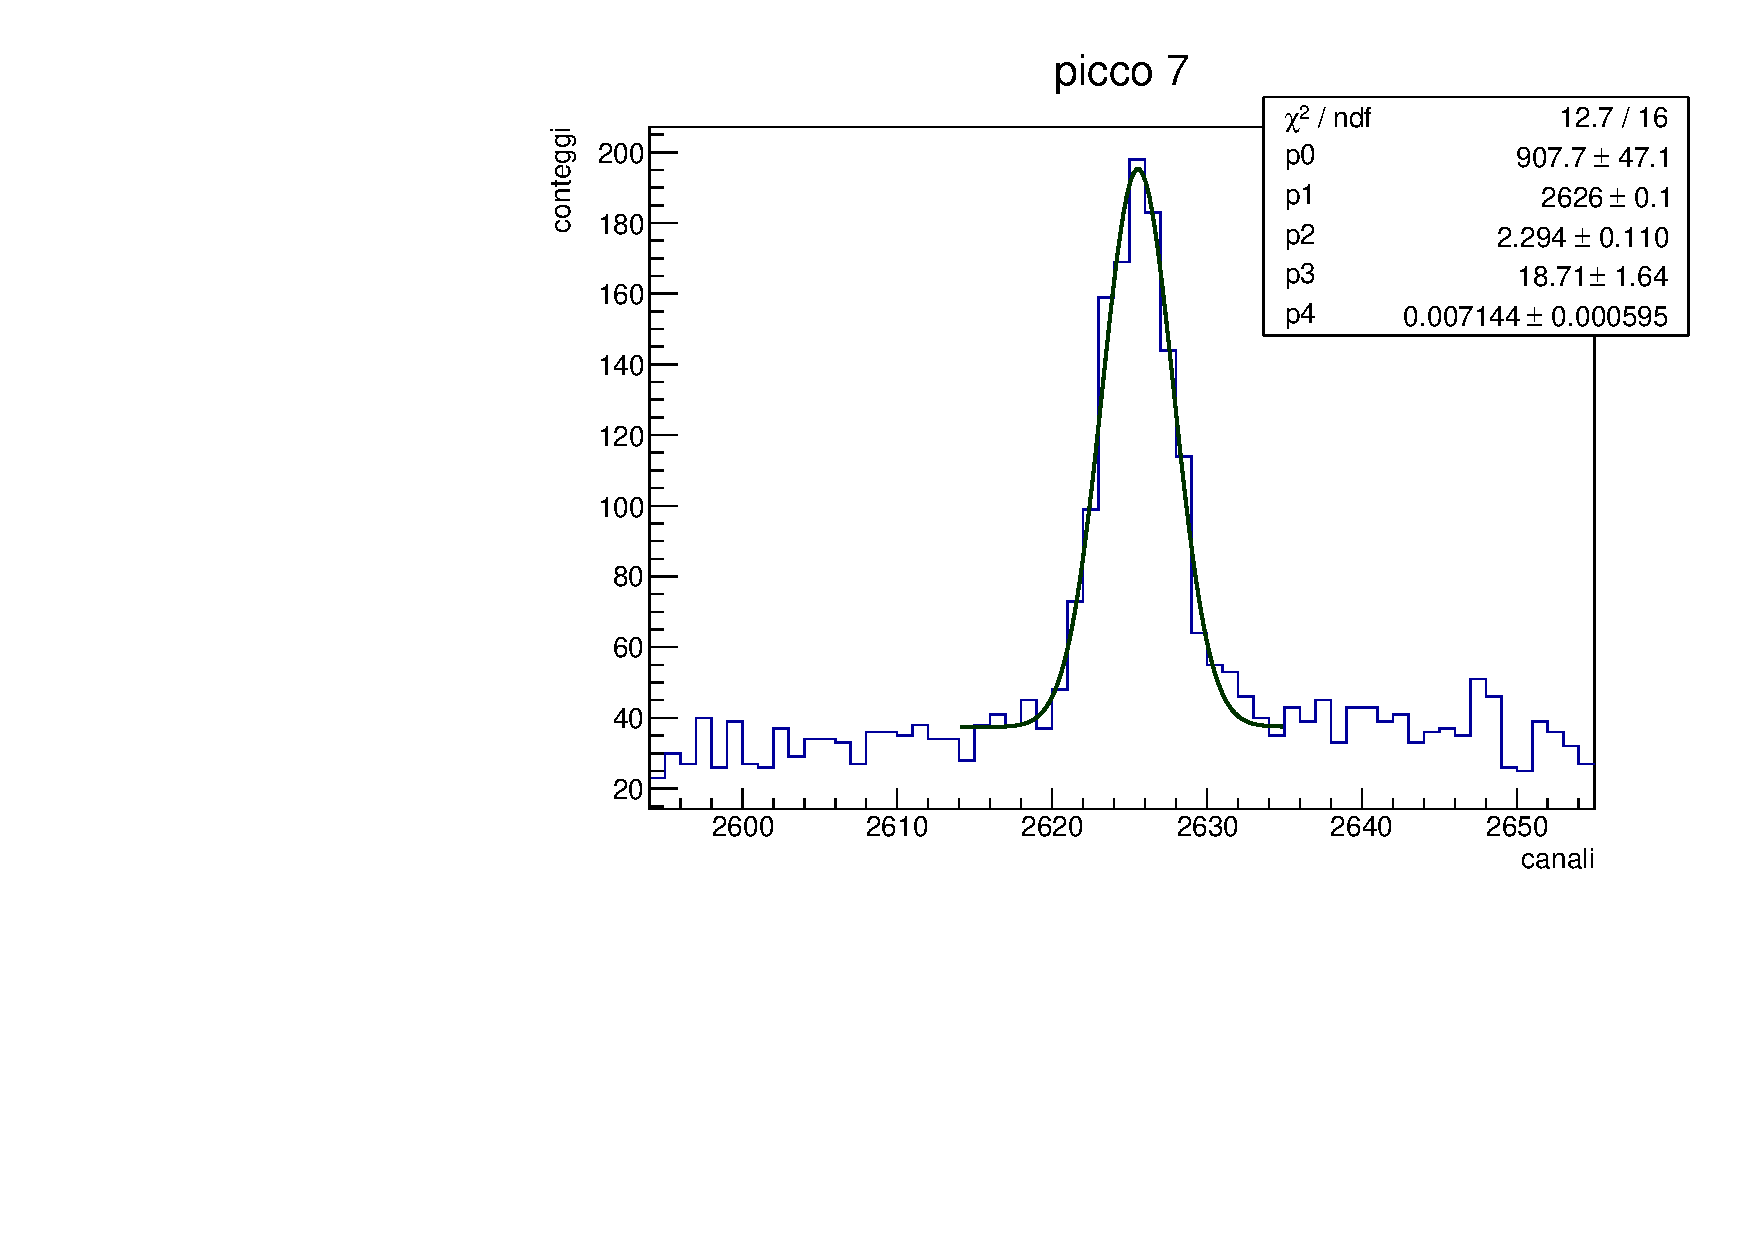
\includegraphics[width=3.4cm]{grafici/picco_europio_germanio_7.pdf}
                    }
                \subfigure[picco 8]
                    {
                        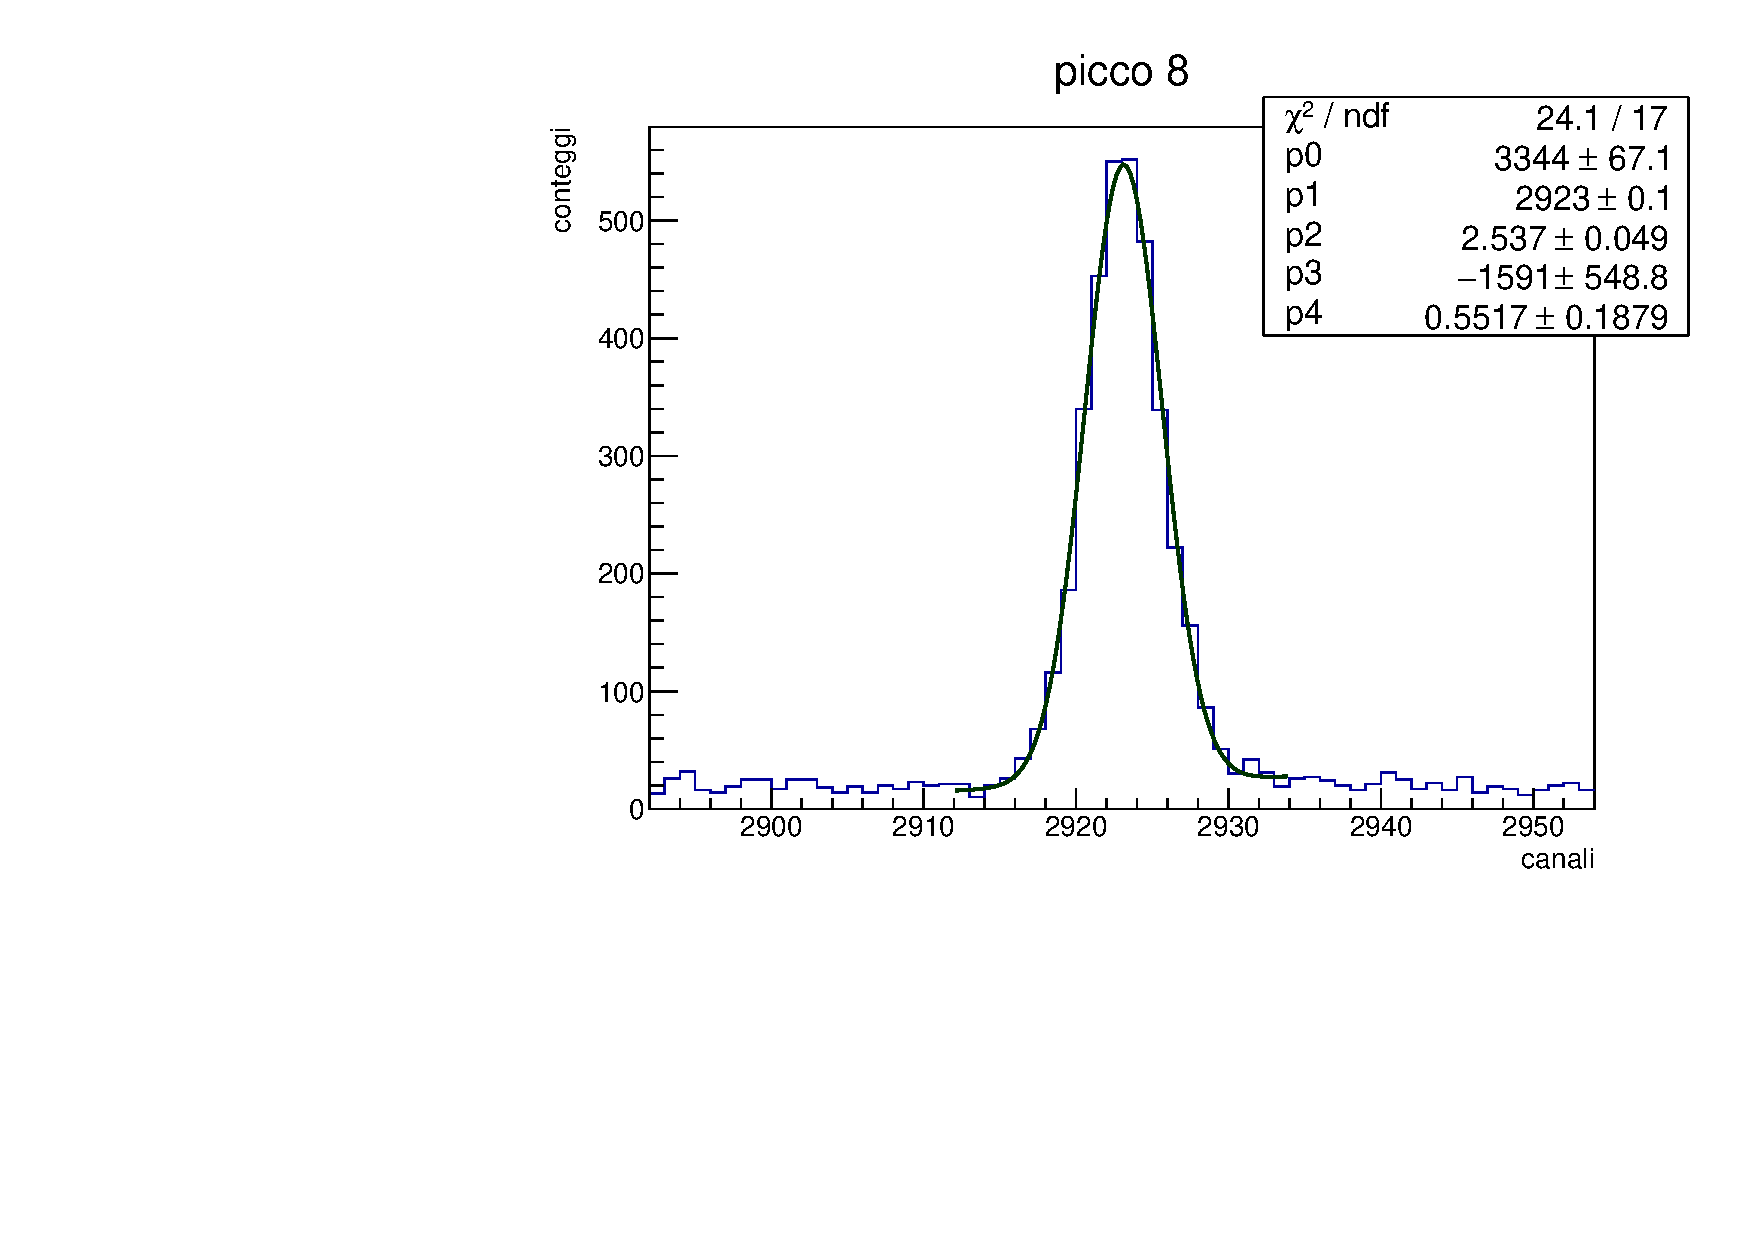
\includegraphics[width=3.4cm]{grafici/picco_europio_germanio_8.pdf}
                    }
                \subfigure[picco 9]
                    {
                        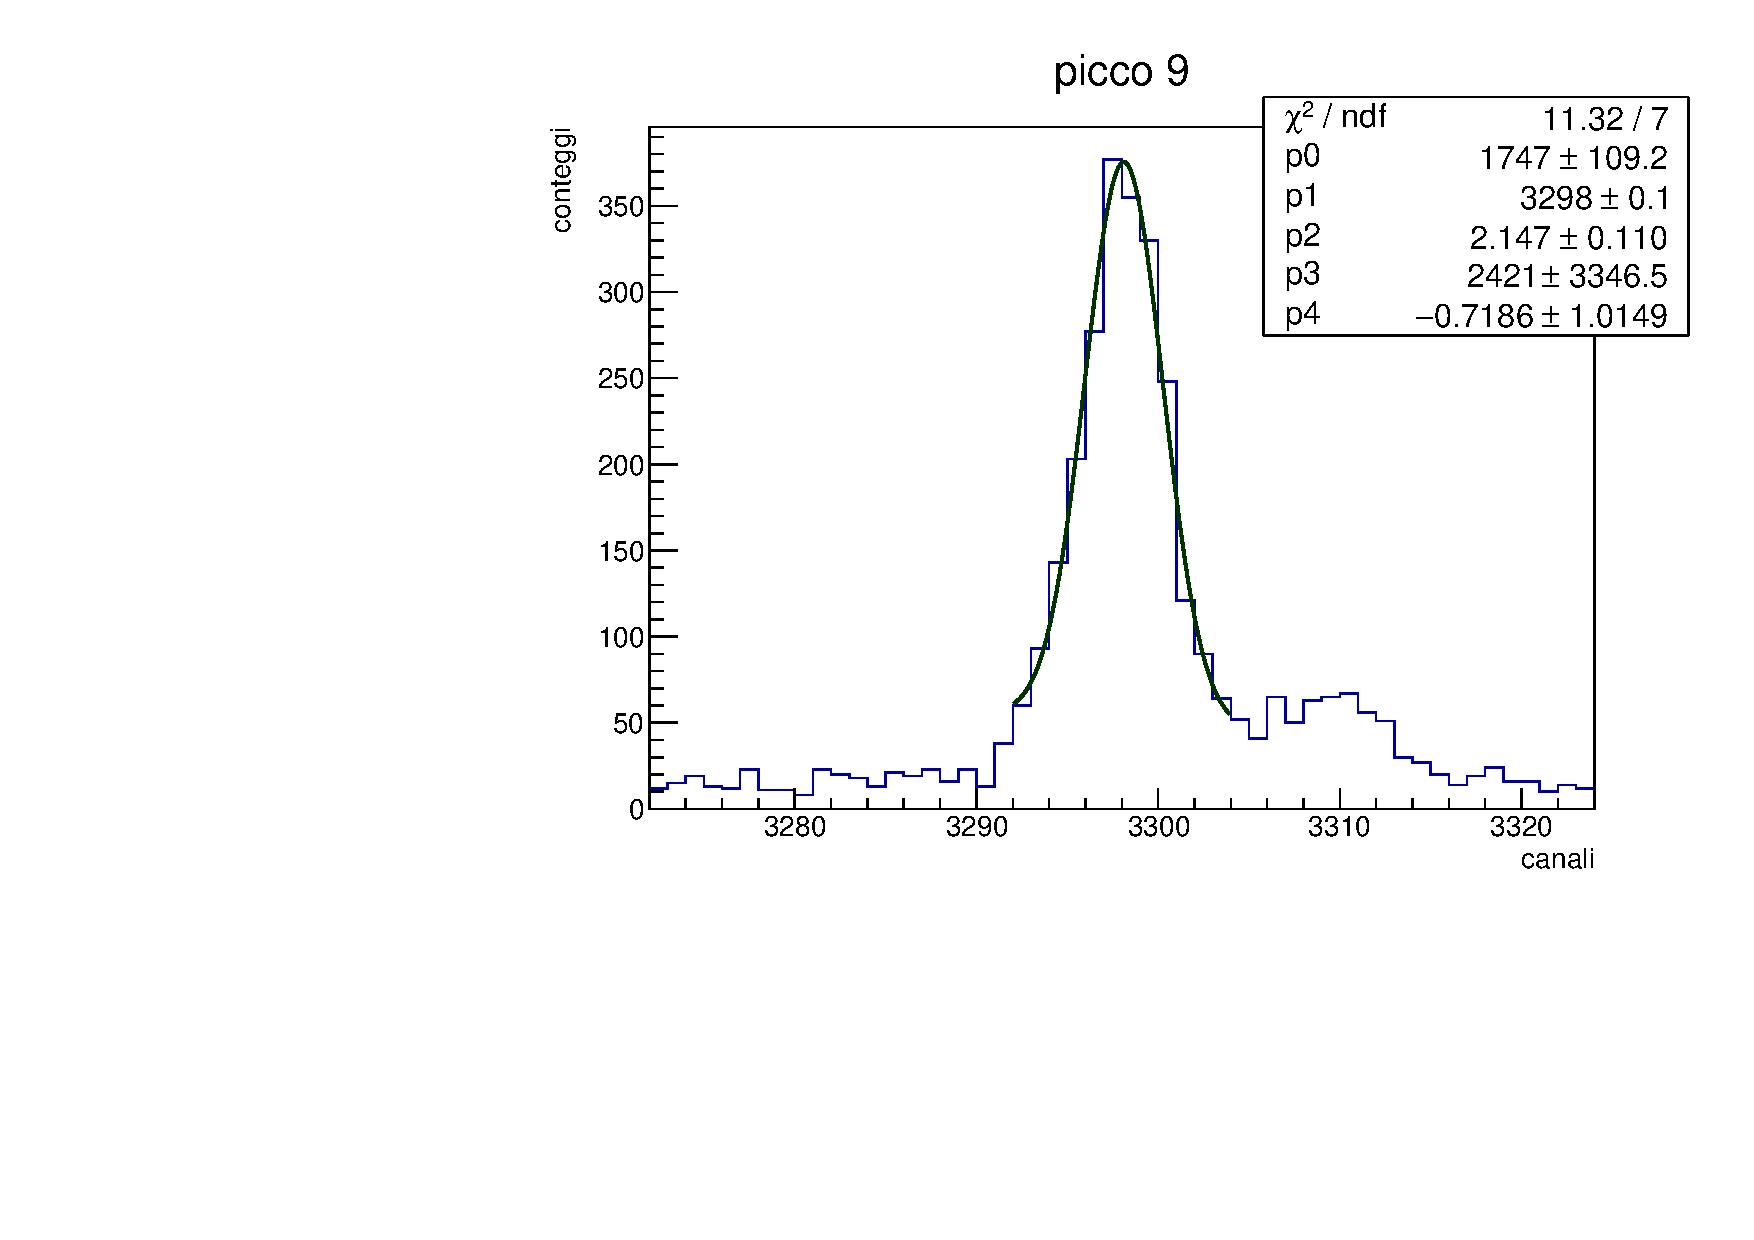
\includegraphics[width=3.4cm]{grafici/picco_europio_germanio_9.pdf}
                    }
                \subfigure[picco 10]
                    {
                        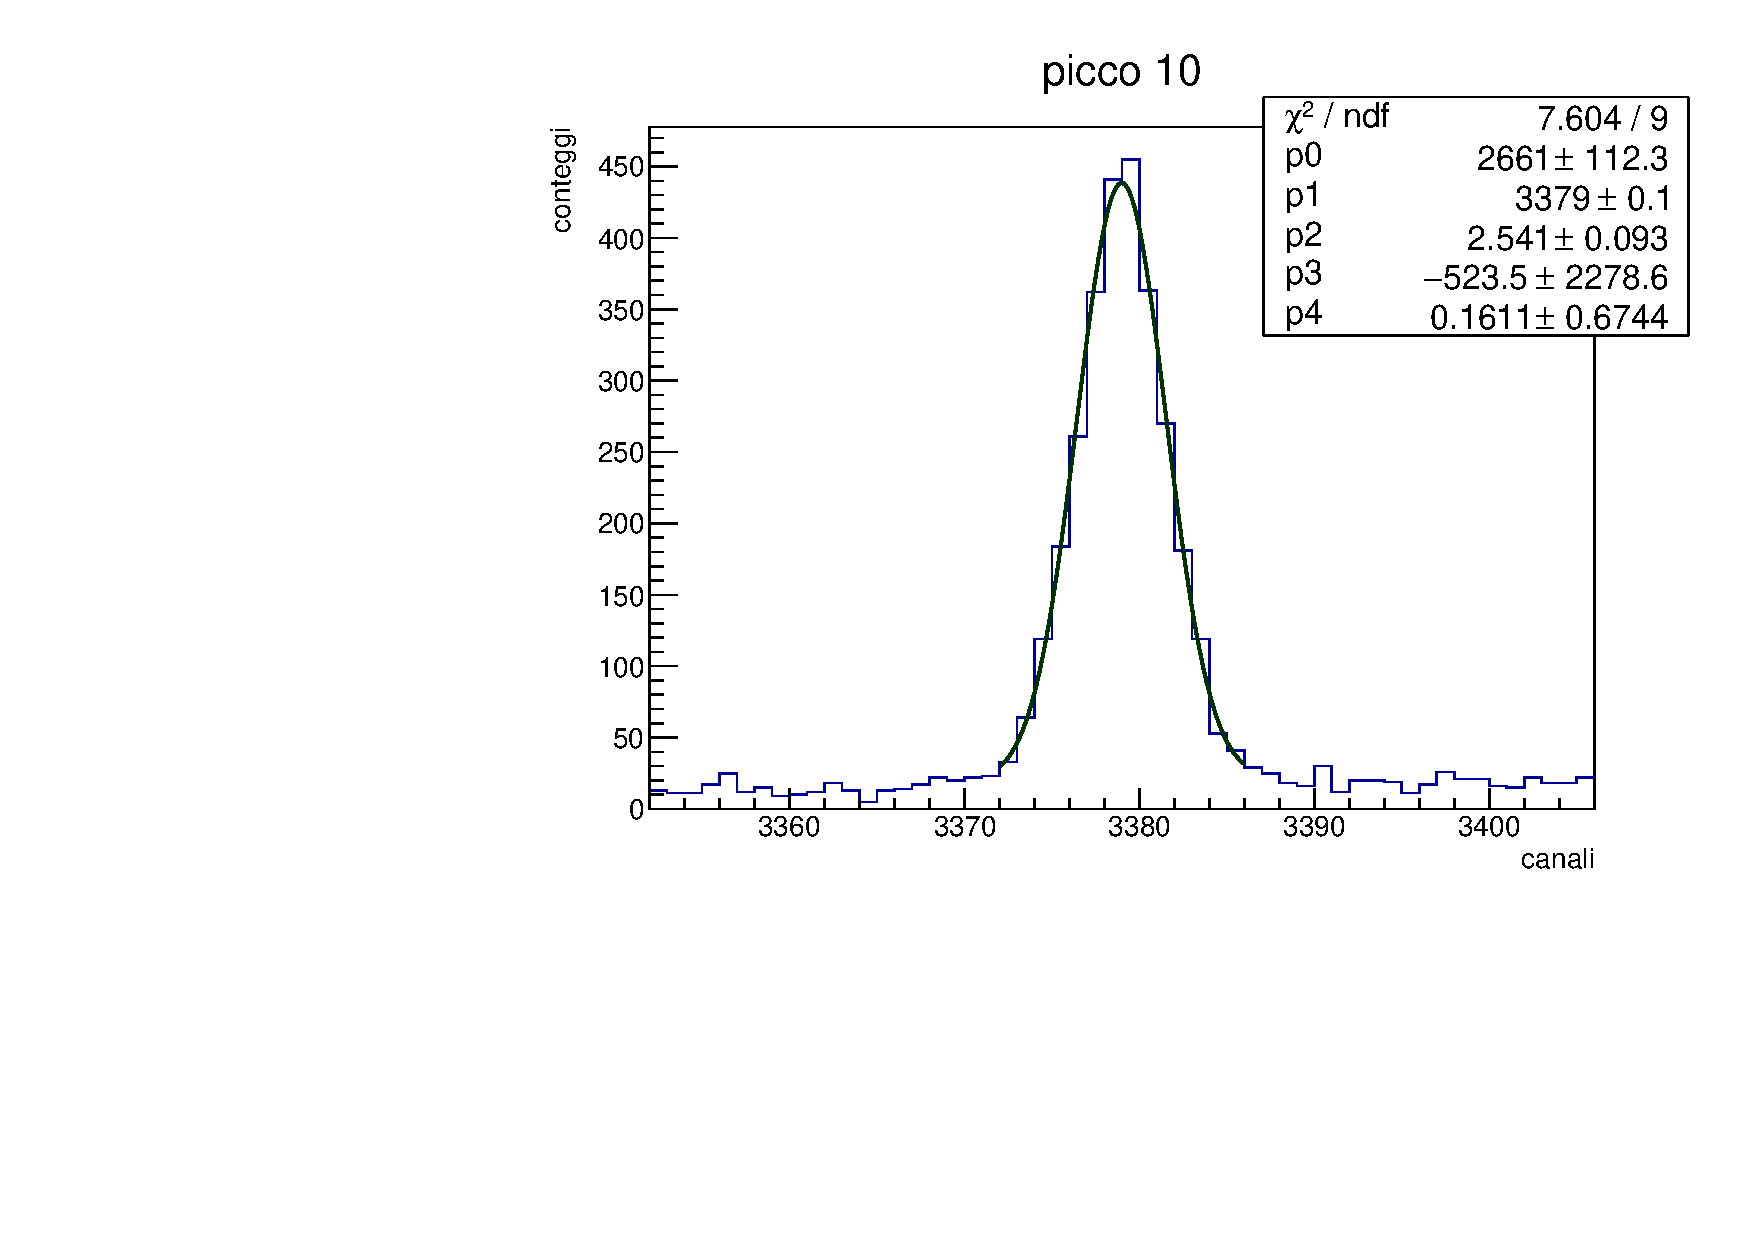
\includegraphics[width=3.4cm]{grafici/picco_europio_germanio_10.pdf}
                    }
                \subfigure[picco 11]
                    {
                        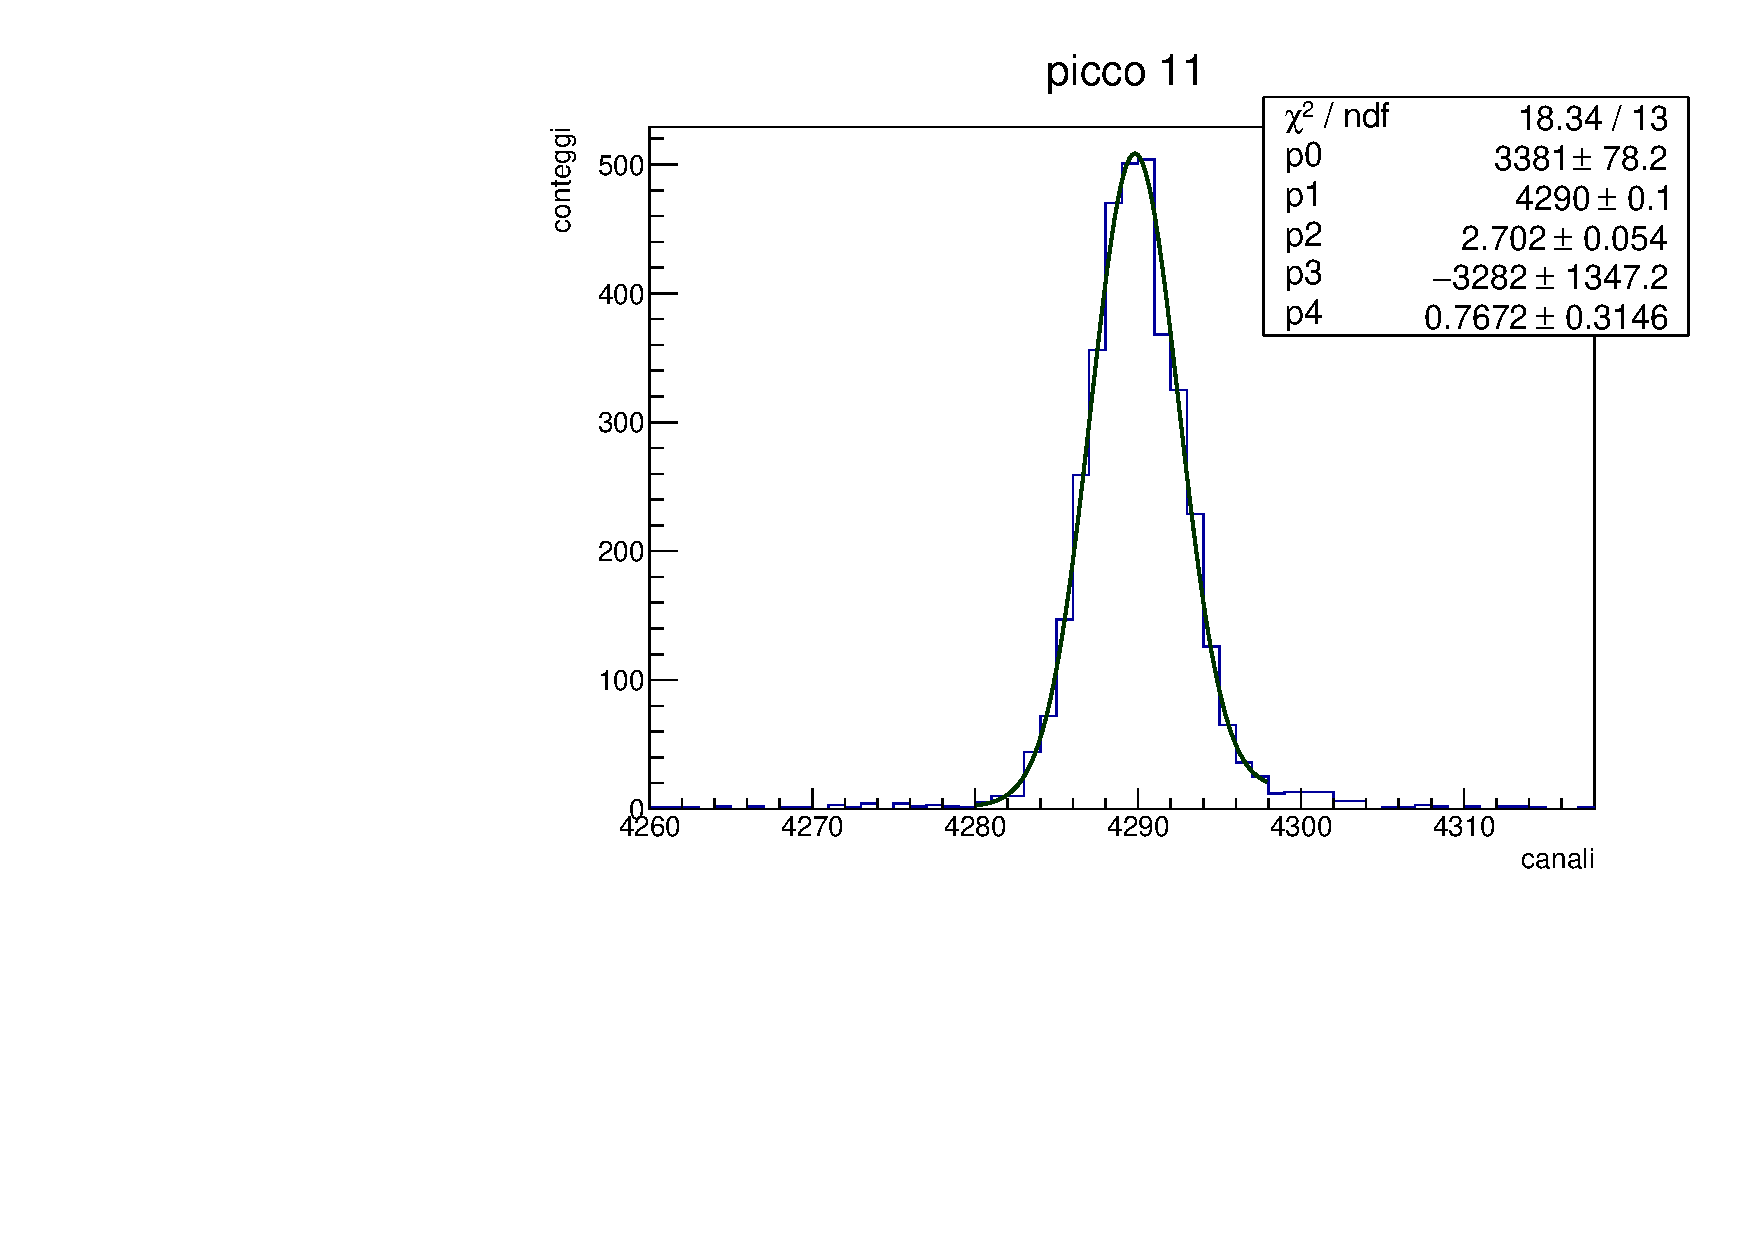
\includegraphics[width=3.4cm]{grafici/picco_europio_germanio_11.pdf}
                    }
            \end{figure}

            \begin{figure}[h!]
                \centering
                \caption{picchi cobalto-60 con fit}
                \label{fig:fit_picchi_cobalto_germanio}
                \subfigure[picco 1]
                    {
                        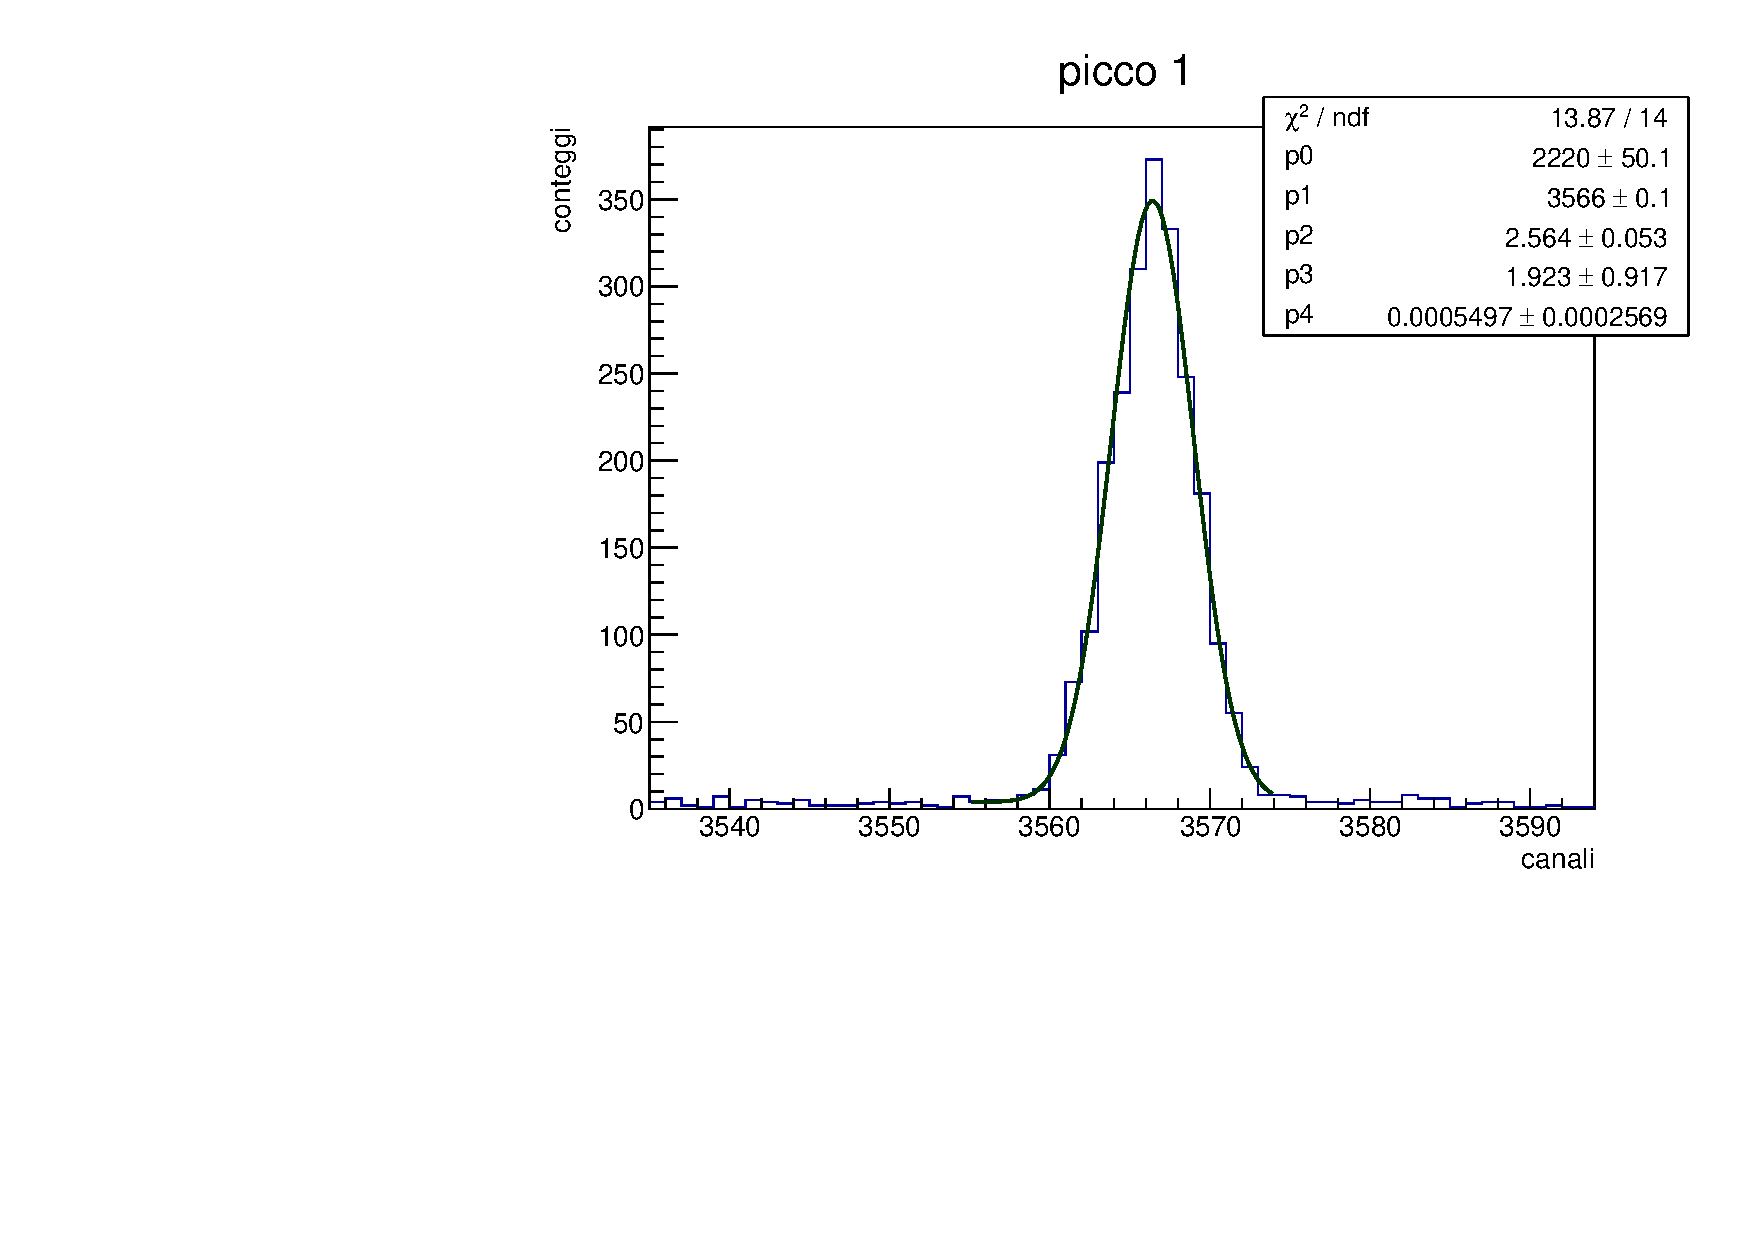
\includegraphics[width=3.4cm]{grafici/picco_cobalto_germanio_1.pdf}
                    }
                \subfigure[picco 2]
                    {
                        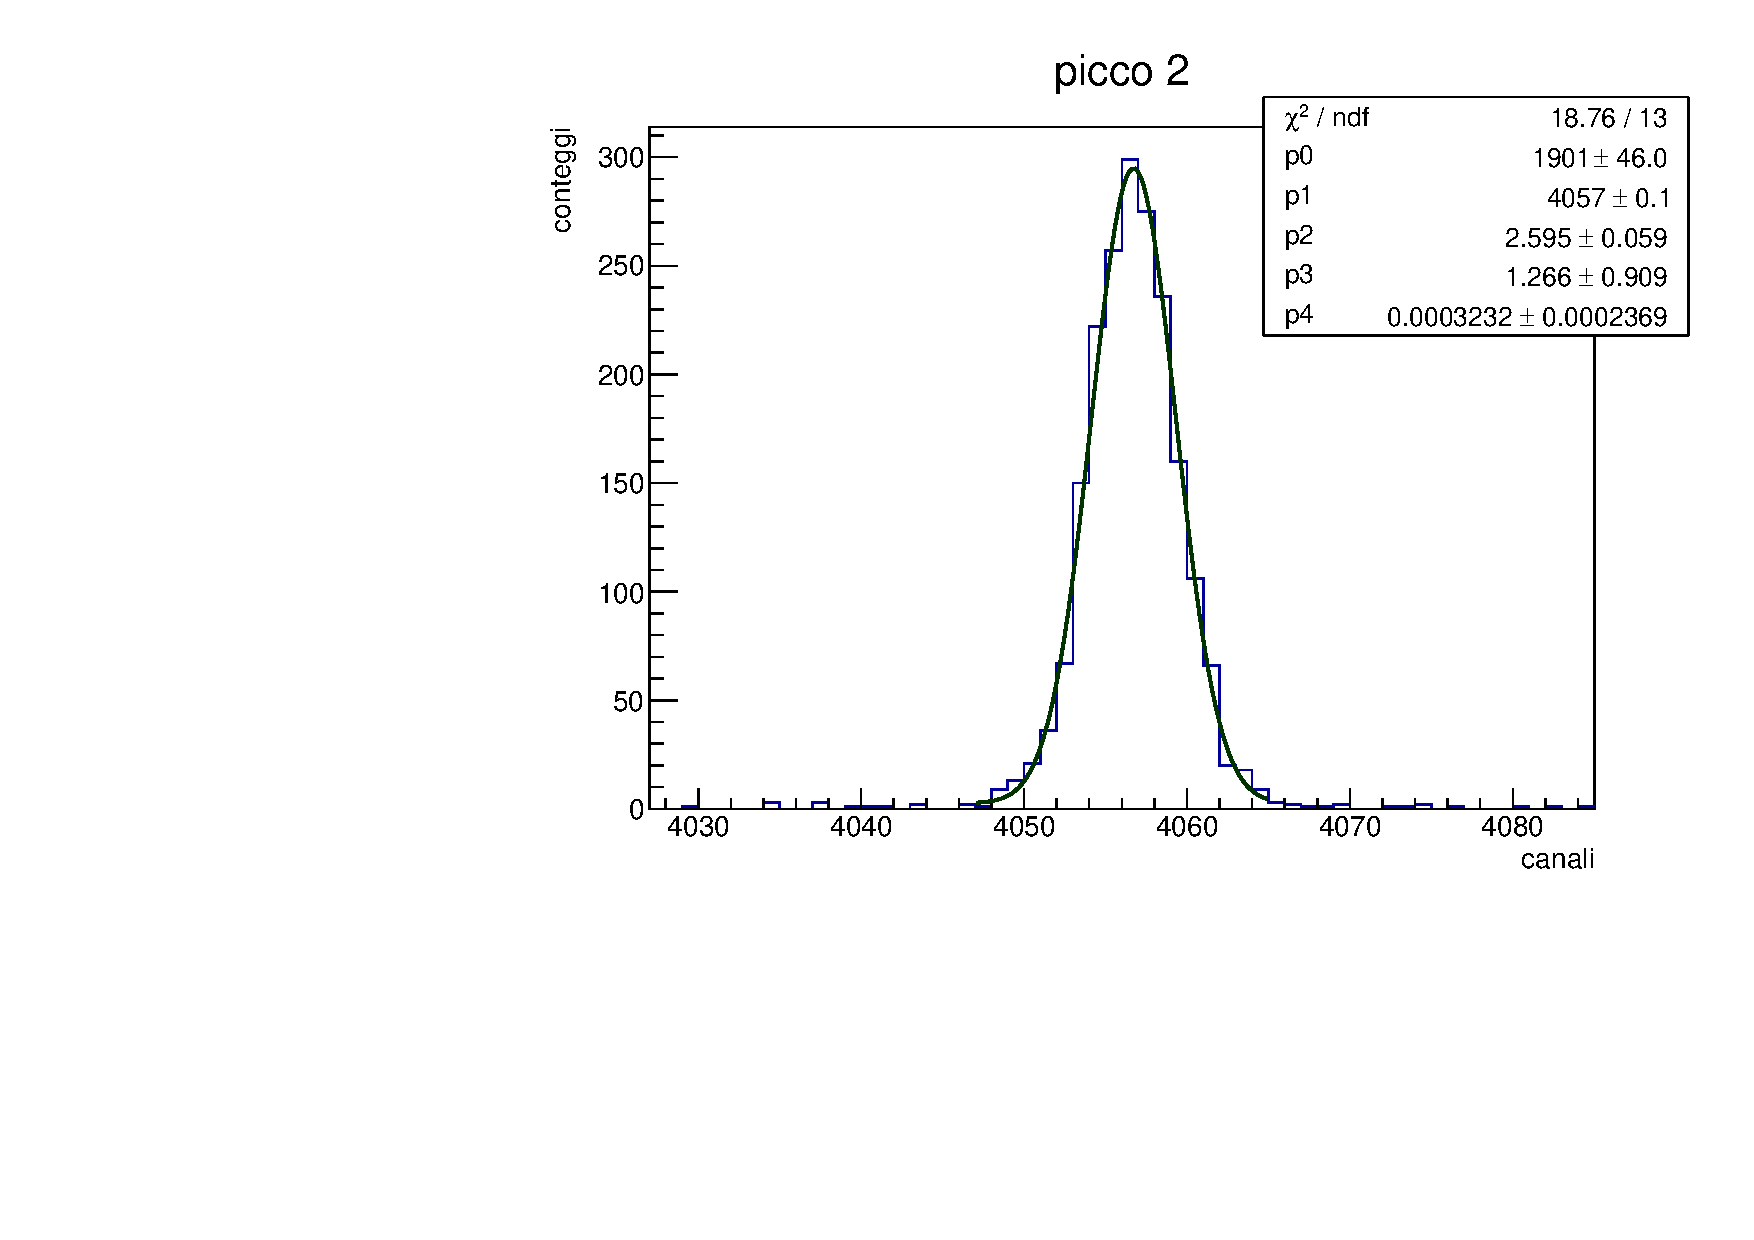
\includegraphics[width=3.4cm]{grafici/picco_cobalto_germanio_2.pdf}
                    }

                \subfigure[picco 1 (alto rateo)]
                    {
                        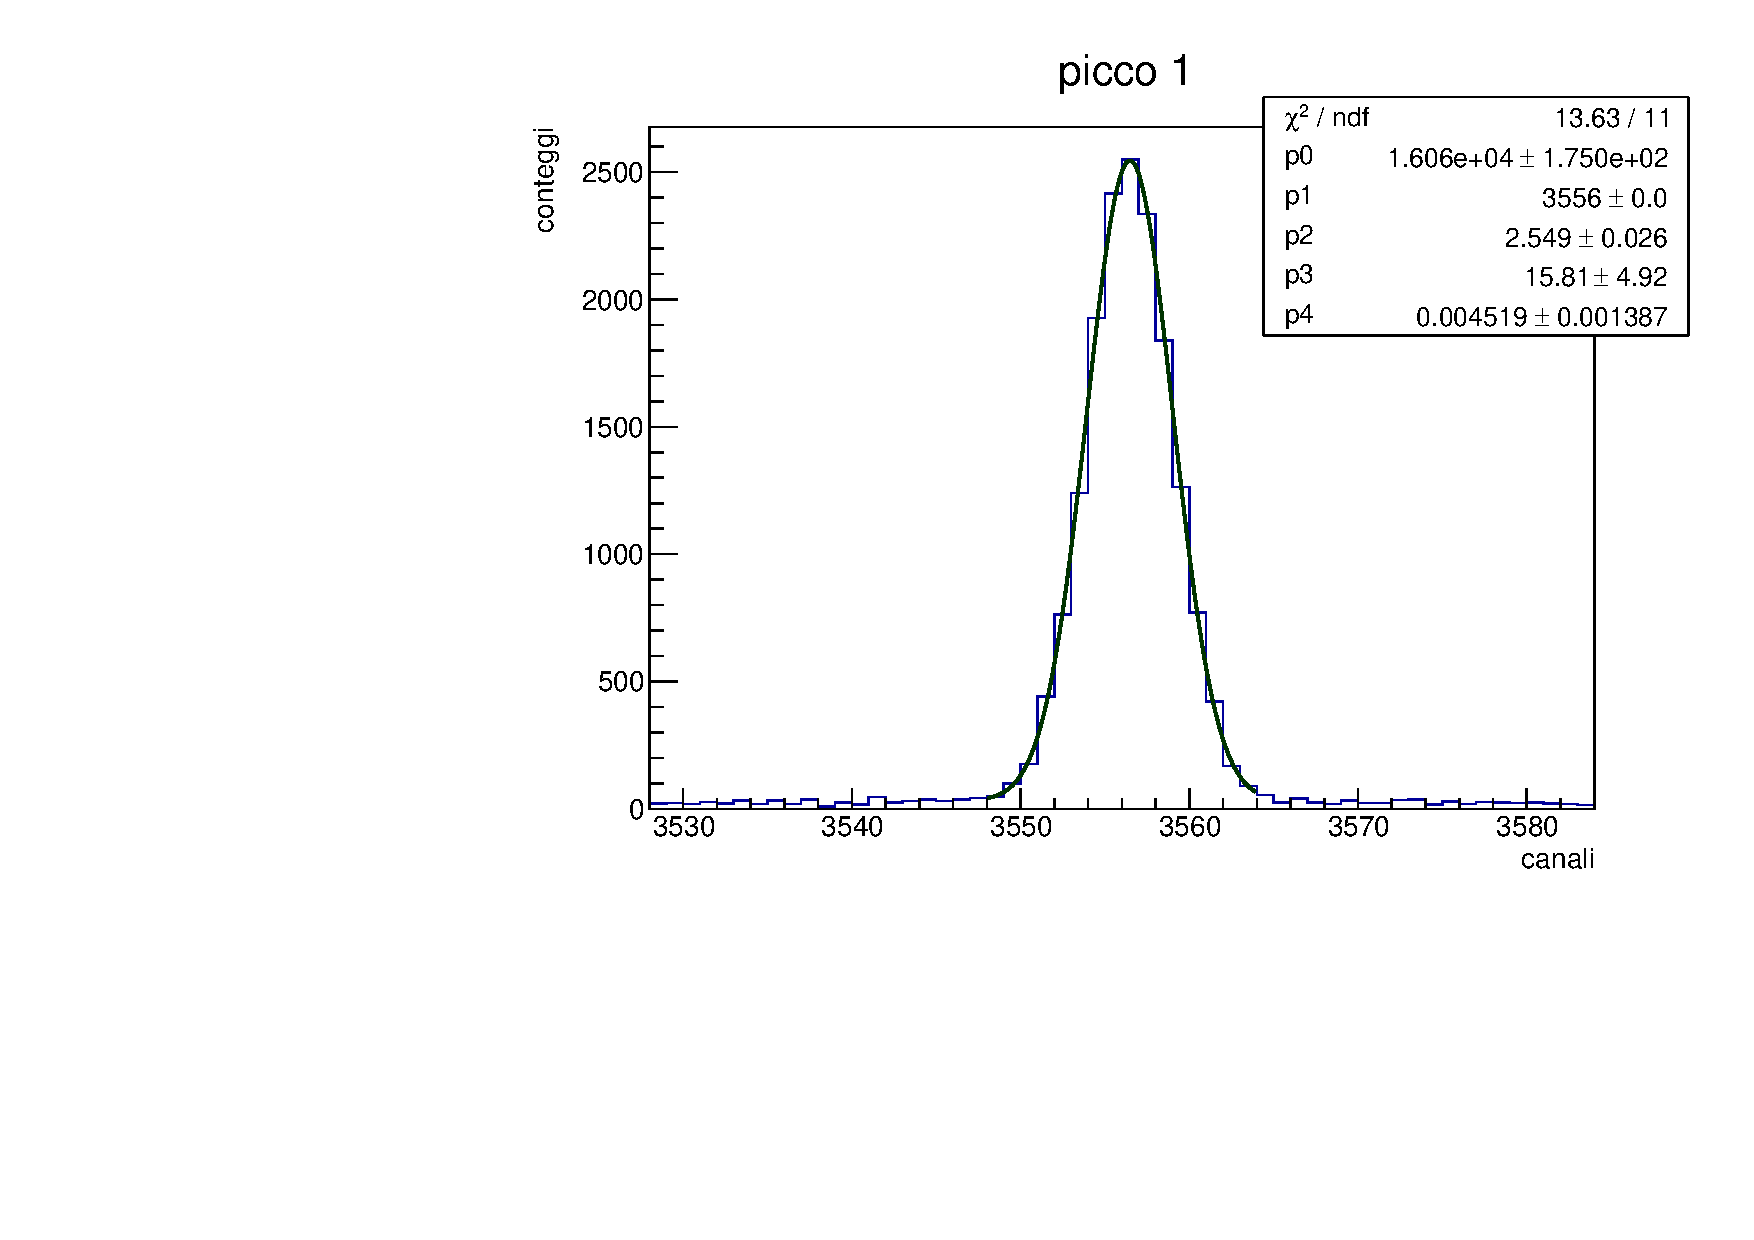
\includegraphics[width=3.4cm]{grafici/picco_cobalto_germanio_highrate_1.pdf}
                    }
                \subfigure[picco 2 (alto rateo)]
                    {
                        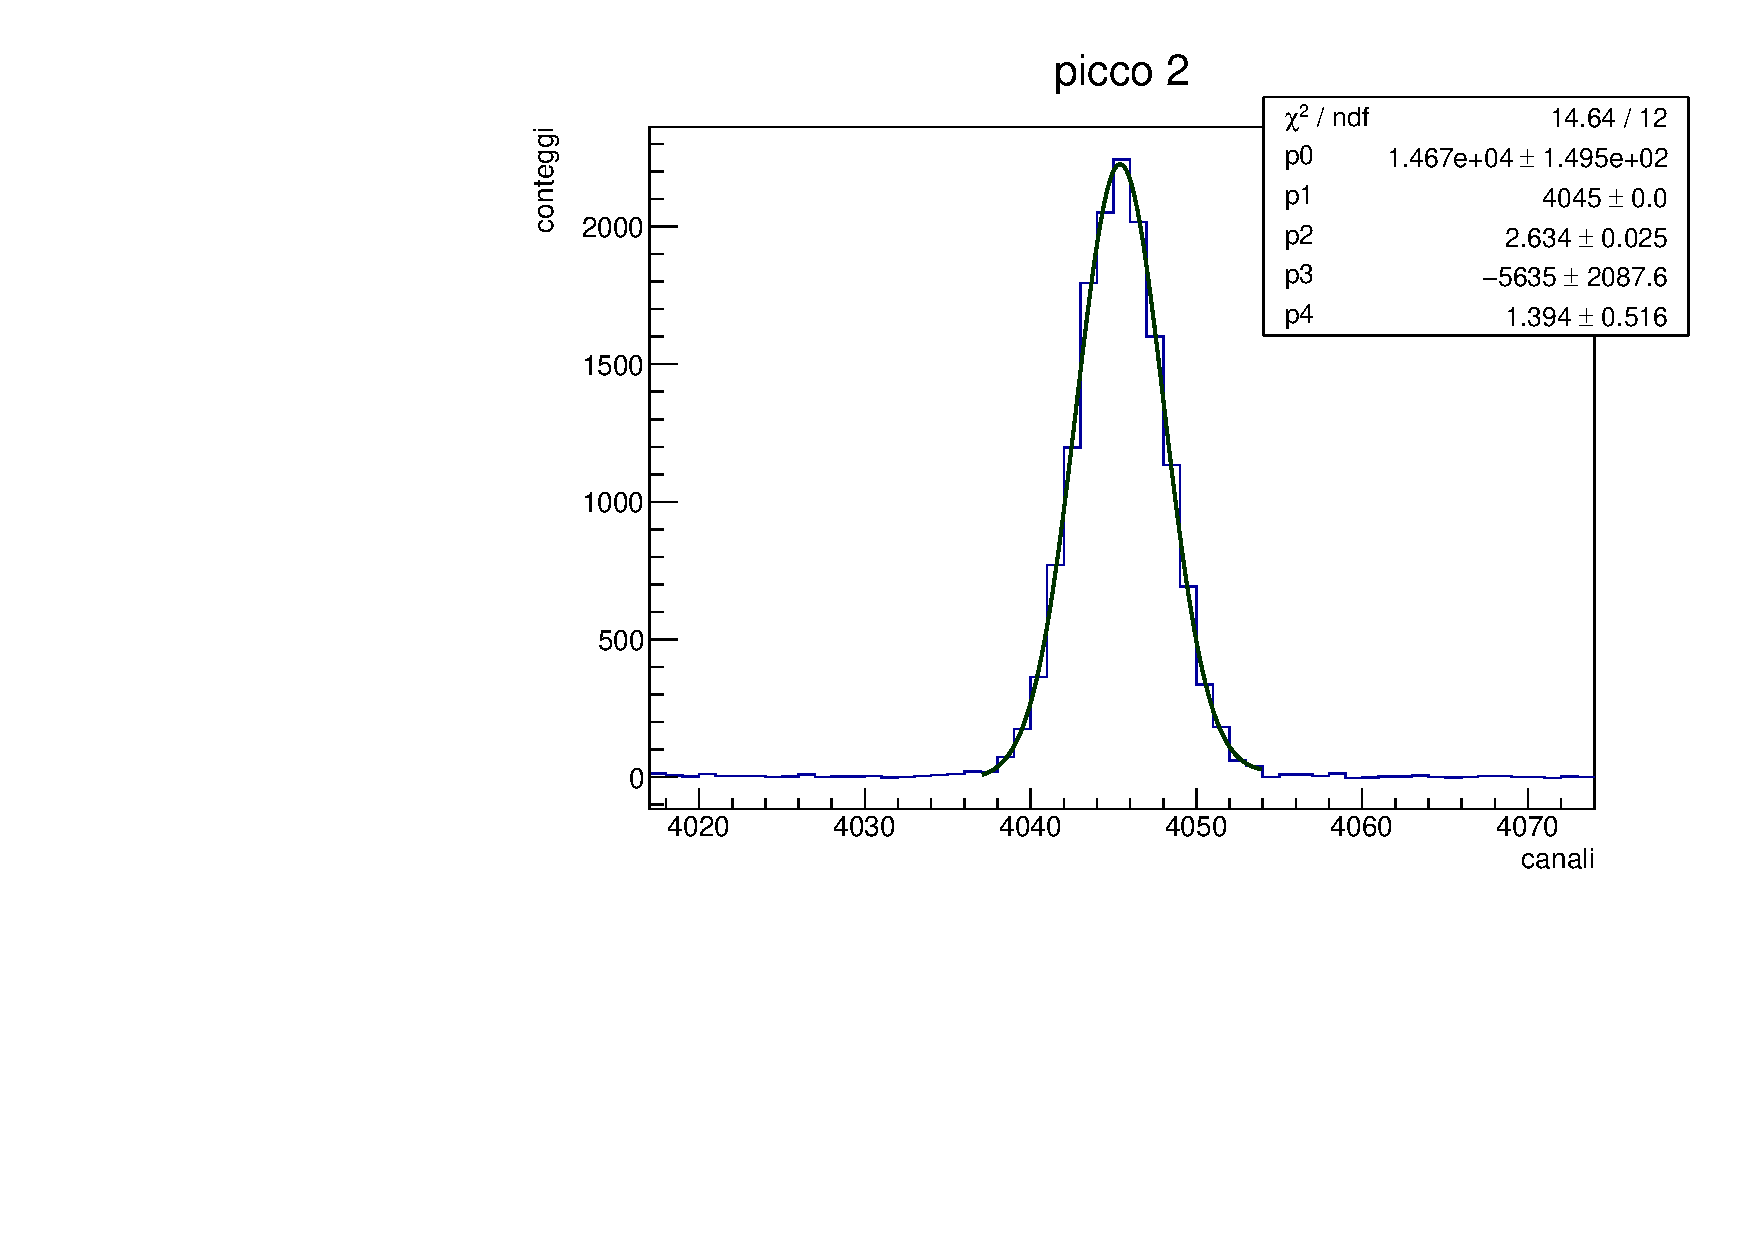
\includegraphics[width=3.4cm]{grafici/picco_cobalto_germanio_highrate_2.pdf}
                    }
            \end{figure}

            \newpage
            La tabella \ref{tab:fit_picchi_europio_cobalto_germanio} mostra, per ciascun picco: conteggi $N$, centroide $X$, deviazione standard $\sigma$, $FWHM$ e la loro corrispondente incertezza $\delta$, e sono anche indicati il valore del $\chi^2$ e dei gradi di libertà $NDF$.

            \begin{table}[h!]
                \centering
                \caption{risultati fit picchi}
                \label{tab:fit_picchi_europio_cobalto_germanio}
                \subtable[fit picchi europio-152\label{tab:fit_picchi_europio_germanio}]
                    {
                        $
                        \begin{array}{ccccccccccc}
	\toprule
	(canali) & N & \delta N & X & \delta X & \sigma & \delta\sigma & FWHM & \delta FWHM & \chi^2 & NDF \\
	\midrule
	\text{picco 1} & 32776 & 199 &  330.142 & 0.012  &  1.889 & 0.010  &  4.449 & 0.024  & 34.72 & 21 \\
	\text{picco 2} & 6684 & 106 &  708.319 & 0.031  &  2.015 & 0.029  &  4.744 & 0.069  & 17.29 & 15 \\
	\text{picco 3} & 17215 & 147 &  1014.909 & 0.018  &  2.035 & 0.015  &  4.792 & 0.036  & 18.22 & 13 \\
	\text{picco 4} & 1127 & 51 &  1220.588 & 0.088  &  2.043 & 0.092  &  4.81 & 0.22  & 19.76 & 15 \\
	\text{picco 5} & 1553 & 69 &  1321.737 & 0.070  &  2.085 & 0.082  &  4.91 & 0.19  & 10.07 & 9 \\
	\text{picco 6} & 3461 & 77 &  2352.910 & 0.048  &  2.250 & 0.047  &  5.30 & 0.11  & 16.65 & 13 \\
	\text{picco 7} & 908 & 47 &  2625.54 & 0.11  &  2.29 & 0.11  &  5.40 & 0.26  & 12.70 & 16 \\
	\text{picco 8} & 3344 & 67 &  2923.117 & 0.051  &  2.537 & 0.049  &  5.97 & 0.11  & 24.10 & 17 \\
	\text{picco 9} & 1747 & 109 &  3298.123 & 0.088  &  2.15 & 0.11  &  5.06 & 0.26  & 11.32 & 7 \\
	\text{picco 10} & 2661 & 112 &  3378.989 & 0.074  &  2.541 & 0.093  &  5.98 & 0.22  & 7.60 & 9 \\
	\text{picco 11} & 3381 & 78 &  4289.793 & 0.058  &  2.702 & 0.054  &  6.36 & 0.13  & 18.34 & 13 \\
	\bottomrule
\end{array}%
                        $
                    }
                \subtable[fit cobalto-60\label{tab:fit_picchi_cobalto_germanio}]
                    {
                        $
                        \begin{array}{ccccccccccc}
	\toprule
	(canali) & N & \delta N & X & \delta X & \sigma & \delta\sigma & FWHM & \delta FWHM & \chi^2 & NDF \\
	\midrule
	\text{picco 1} & 2220 & 50 &  3566.422 & 0.058  &  2.564 & 0.053  &  6.04 & 0.12  & 13.87 & 14 \\
	\text{picco 2} & 1901 & 46 &  4056.727 & 0.062  &  2.595 & 0.059  &  6.11 & 0.14  & 18.76 & 13 \\
	\bottomrule
\end{array}%
                        $
                    }
                \subtable[fit cobalto-60 (alto rateo)\label{tab:fit_picchi_cobalto_germanio_highrate}]
                    {
                        $
                        \begin{array}{ccccccccccc}
	\toprule
	(canali) & N & \delta N & X & \delta X & \sigma & \delta\sigma & FWHM & \delta FWHM & \chi^2 & NDF \\
	\midrule
	\text{picco 1} & 16062 & 175 &  3556.479 & 0.022  &  2.549 & 0.026  &  6.002 & 0.061  & 13.63 & 11 \\
	\text{picco 2} & 14671 & 150 &  4045.397 & 0.026  &  2.634 & 0.025  &  6.201 & 0.058  & 14.64 & 12 \\
	\bottomrule
\end{array}%
                        $
                    }
                
            \end{table}
            
            \newpage
            La tabella \ref{tab:fit_calibrazione_provvisoria} mostra il fit lineare provvisorio, come nella \eqref{for:fit_calibrazione_provvisoria}, e le energie provvisorie corrispondenti utili per l'identificazione dei picchi (solo per l'europio-152, dato che nel cobalto-60 vi sono solo due picchi con ovvia corrispondenza).
            
            \begin{table}[h!]
                \centering
                \caption{fit lineare provvisorio con picchi cobalto-60}
                \label{tab:fit_calibrazione_provvisoria}
                \subtable[fit lineare provvisorio]
                    {
                        $
                        \begin{array}{cc}
                            (canali\:/\:\si{\kilo\electronvolt})&(canali)\\
                            \toprule
                            \beta_0       & \alpha_0      \\
                            \midrule
                            0.32&16.15\\
                            \bottomrule
                        \end{array}
                        $
                    }
                \subtable[energie provvisorie]
                    {
                        $
                        \begin{array}{cc}
                            \toprule
                            \si{(\kilo\electronvolt)}       & E_0        \\
                            \midrule
                            \text{picco 1}&121.78\\
                            \text{picco 2}&244.78\\
                            \text{picco 3}&344.88\\
                            \text{picco 4}&406.69\\
                            \text{picco 5}&439.04\\
                            \text{picco 6}&768.99\\
                            \text{picco 7}&856.21\\
                            \text{picco 8}&951.43\\
                            \text{picco 9}&1071.42\\
                            \text{picco 10}&1097.29\\
                            \text{picco 11}&1388.72\\
                            \bottomrule
                        \end{array}
                        $
                    }
            \end{table}

            \newpage
            Infine, la tabella \ref{tab:fit_calibrazione} e la figura \ref{fig:fit_calibrazione} mostrano i risultati del fit lineare definitivo per la calibrazione $E=\alpha + \beta X$.

            \begin{table}[h!]
                \centering
                \caption{fit calibrazione definitivo}
                \label{tab:fit_calibrazione}
                $
                \begin{array}{cccccc}
	\toprule
	\alpha & \delta\alpha & \beta & \delta\beta & \chi^2 & NDF \\
	\midrule
	 14.5468 & 0.0038  &  0.3248607 & 0.0000027  & 194.33 & 11 \\
	\bottomrule
\end{array}

                $
            \end{table}
            
            \begin{figure}[h!]
                \centering
                \caption{fit lineare calibrazione}
                \label{fig:fit_calibrazione}
                \subfigure[fit lineare]
                    {
                        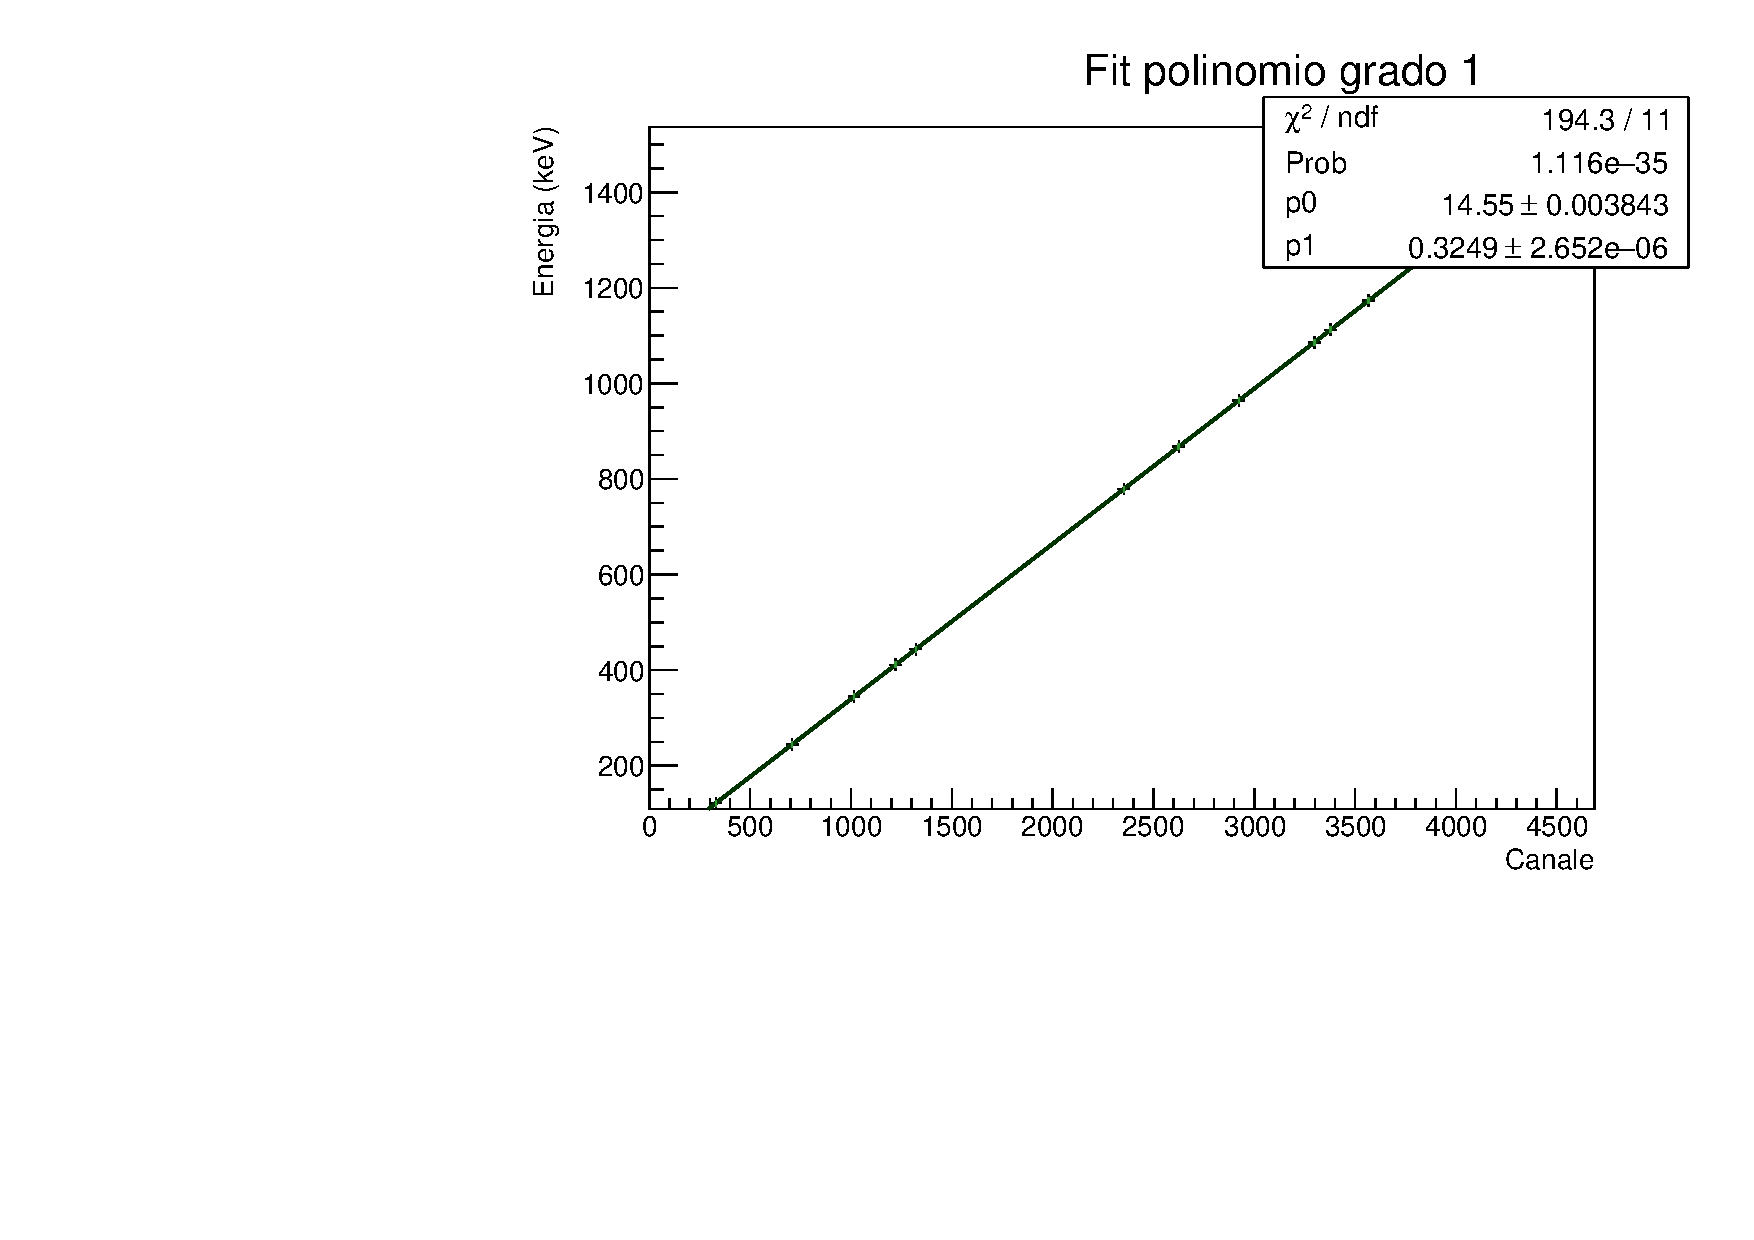
\includegraphics[width=7cm]{grafici/fit_calibrazione.pdf}
                    }
                \subfigure[andamento residui]
                    {
                        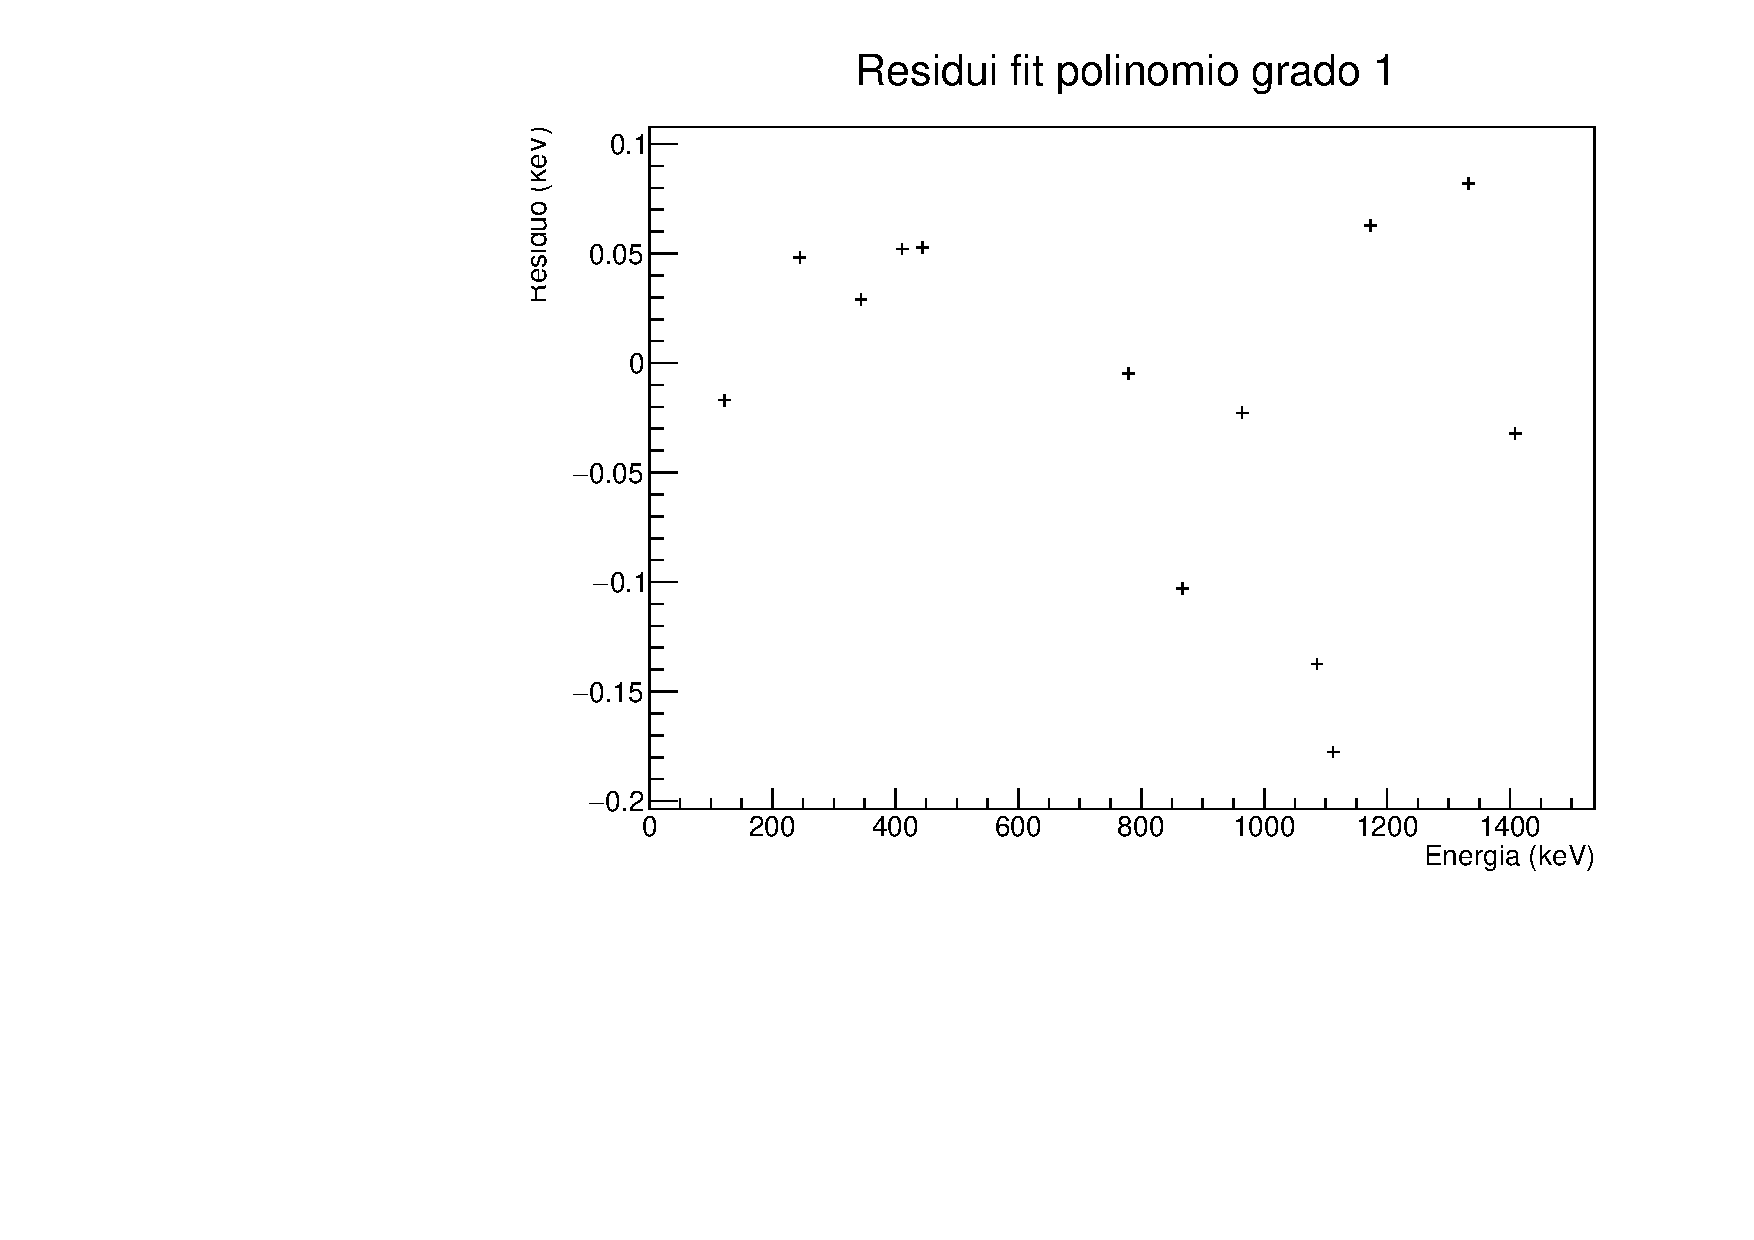
\includegraphics[width=7cm]{grafici/fit_calibrazione_residui.pdf}
                    }
            \end{figure}

            L'andamento casuale dei residui rispetto all'energia tabulata mostra che una funzione polinomiale di grado 1 è sufficiente, per cui non ha significato aumentarne il grado: la calibrazione è effettivamente lineare.

        \section{La risoluzione}
            Una volta effettuata la calibrazione, è possibile convertire i risultati utili del fit in canali per ottenere i corrispondenti valori di energia per ciascun picco, quindi calcolarne le risoluzioni per studiarne l'andamento mediante un best fit con la relazione \eqref{for:fit_risoluzione}.

            Per farlo, è possibile sfruttare dei codici che sono in grado di convertire i risultati 

            \subsection*{Il funzionamento del codice}
            Questa procedura di analisi dati ha richiesto l'utilizzo di un codice:
                \begin{itemize}
                    \item La macro \textit{fit\_risoluzione.cpp} è in grado di calcolare la risoluzione in energia di ciascun picco e di eseguirne il best fit con le energie tabulate rispetto alla formula \ref{for:fit_risoluzione}.

                    \textbf{Input}: risultati FWHM della macro \textit{spettro.cpp} ed energie tabulate in un file di testo.
                    
                    \textbf{Output}: plot fit caratteristico della risoluzione rispetto all'energia in un file pdf e risultati numerici con risoluzioni in file di testo.
                \end{itemize}
                \subsubsection*{Note operative}
                    La macro \textit{fit\_calibrazione.cpp} ha un solo file di input, per cui, se si vogliono considerare sia l'europio-152 che il cobalto-60 nel fit delle risoluzioni, bisogna unire manualmente i risultati per le due sorgenti.
                    
            \subsection*{La propagazione delle incertezze}
                \subsubsection*{La conversione in energia}
                    L'incertezza dei parametri $a$, $b$ e $c$ che appaiono nel fit caratteristico \eqref{for:fit_risoluzione} è data direttamente dal codice dal comando \textit{GetParError()}.
                    Invece, per quanto riguarda la conversione in energie, una volta noti i risultati dei fit gaussiani in canali e i parametri della retta di calibrazione, bisogna calcolare i valori utili in \si{\kilo\electronvolt}, ovvero l'energia $E$ e la $FWHM$ con la corrispondente incertezza:
                    \begin{align*}
                        &E=\beta\cdot X+\alpha&&\Rightarrow&&\delta E=\sqrt{\delta\alpha^2+(X\cdot\delta\beta)^2+(\beta\cdot\delta X)^2}\\
                        &FWHM_{\text{en}}=\beta\cdot FWHM_{\text{ch}}&&\Rightarrow&&\delta FWHM_{\text{en}}=\sqrt{(FWHM_{\text{ch}}\cdot\delta\beta)^2+(\beta\cdot FWHM_{\text{ch}})^2}
                    \end{align*}                    

            \subsection*{I risultati ottenuti}
                La tabella \ref{tab:risoluzioni} mostra, per l'europio-152 e per il cobalto-60, le risoluzioni in energia di ciascun picco con la corrispondente incertezza, mentre la figura \ref{fig:fit_risoluzione} e la tabella \ref{tab:fit_risoluzione} mostrano i risultati del loro fit caratteristico, secondo la formula \eqref{for:fit_risoluzione}.
                \begin{table}[h!]
                    \centering
                    \caption{risoluzioni in energia}
                    \label{tab:risoluzioni}
                    \subtable[Europio-152]
                        {
                            $
                            \begin{array}{ccc}
	\toprule
	\% & R & \delta R \\
	\midrule
	\text{picco 1} & 1.1832 & 0.0064  \\
	\text{picco 2} & 0.6279 & 0.0091  \\
	\text{picco 3} & 0.4508 & 0.0034  \\
	\text{picco 4} & 0.379 & 0.017  \\
	\text{picco 5} & 0.358 & 0.014  \\
	\text{picco 6} & 0.2203 & 0.0046  \\
	\text{picco 7} & 0.2017 & 0.0096  \\
	\text{picco 8} & 0.2007 & 0.0038  \\
	\text{picco 9} & 0.1508 & 0.0078  \\
	\text{picco 10} & 0.1743 & 0.0064  \\
	\text{picco 11} & 0.1464 & 0.0029  \\
	\bottomrule
\end{array}

                            $
                        }
                    \subtable[Cobalto-60]
                        {
                            $
                            \begin{array}{ccc}
	\toprule
	\% & R & \delta R \\
	\midrule
	\text{picco 1} & 0.1667 & 0.0034  \\
	\text{picco 2} & 0.1485 & 0.0034  \\
	\bottomrule
\end{array}

                            $
                        }
                    \subtable[Cobalto-60 (alto rateo)]
                        {
                            $
                            \begin{array}{ccc}
	\toprule
	\% & R & \delta R \\
	\midrule
	\text{picco 1} & 0.0546 & 0.0012  \\
	\text{picco 2} & 0.01558 & 0.00035  \\
	\bottomrule
\end{array}

                            $
                        }
                \end{table}
                
                \begin{table}[h!]
                    \centering
                    \caption{fit caratteristico risoluzione}
                    \label{tab:fit_risoluzione}
                    $
                    \begin{array}{cccccccc}
	\toprule
	a & \delta a & b & \delta b & c & \delta c & \chi^2 & NDF \\
	\midrule
	 1.904 & 0.042  &  0.00145 & 0.00023  &  0.00000012 & 0.00000018  & 20.84 & 10 \\
	\bottomrule
\end{array}

                    $
                \end{table}
                
                \begin{figure}[h!]
                    \centering
                    \caption{fit risoluzioni con energie tabulate}
                    \label{fig:fit_risoluzione}
                    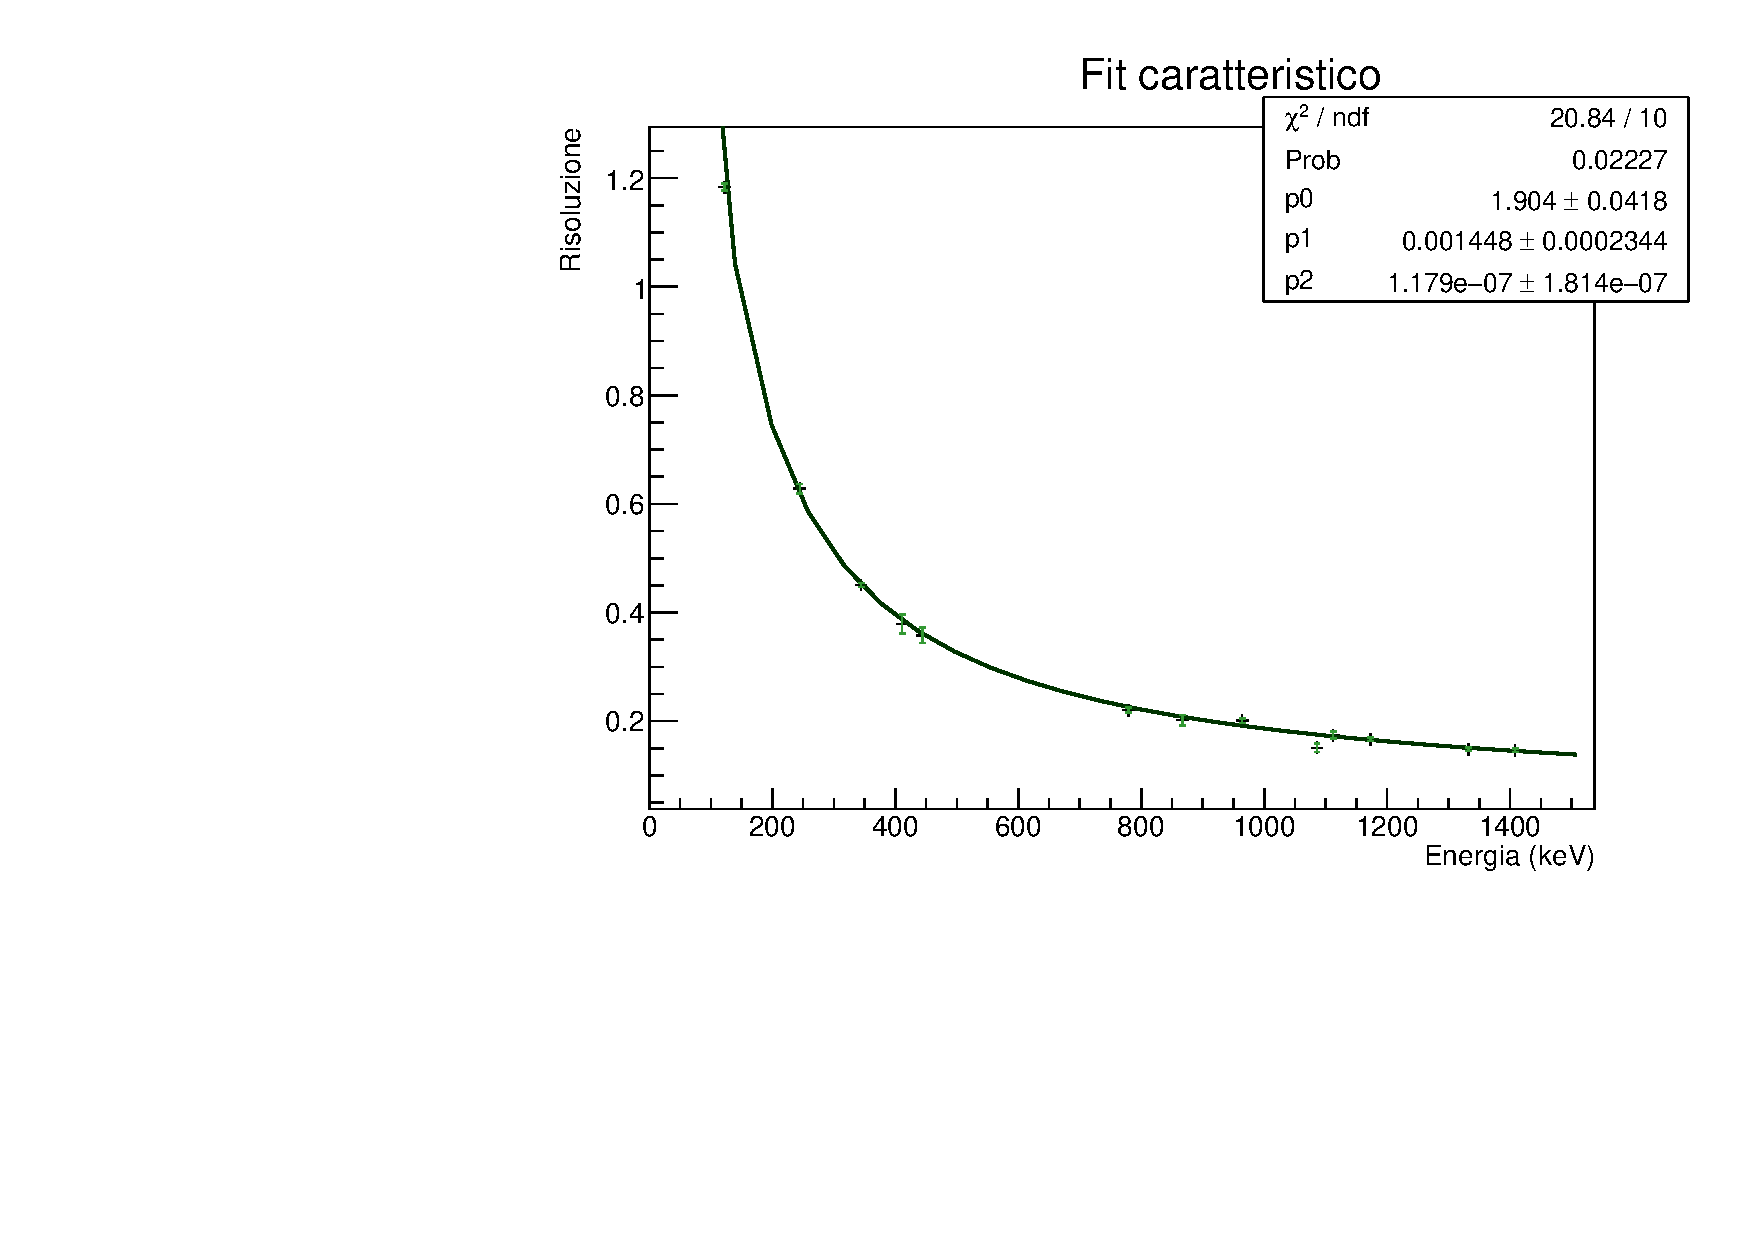
\includegraphics[width=10cm]{grafici/fit_risoluzione.pdf}
                \end{figure}
            
        \newpage
        \section{Il rumore elettronico}
            Anche quando il segnale è dato dal solo pulser, l'apparato sperimentale fornisce uno spettro in formato di testo, che può essere studiato con lo stesso codice usato in precedenza, nonché la macro \textit{spettro.cpp}. Ai fini dell'esperimento, ciò che serve dal picco gaussiano del pulser è la sua $FWHM$ con la corrispondente incertezza, per cui il funzionamento del codice è identico e bisogna cambiare solamente il nome dei file di input e di output.

            \subsection*{I risultati ottenuti}
                La figura \ref{fig:picco_pulser_germanio} e la tabella \ref{tab:fit_picco_pulser_germanio} mostrano i risultati del fit per il picco del pulser. 
                \begin{figure}[h!]
                    \centering
                    \caption{picco pulser con fit}
                    \label{fig:picco_pulser_germanio}
                    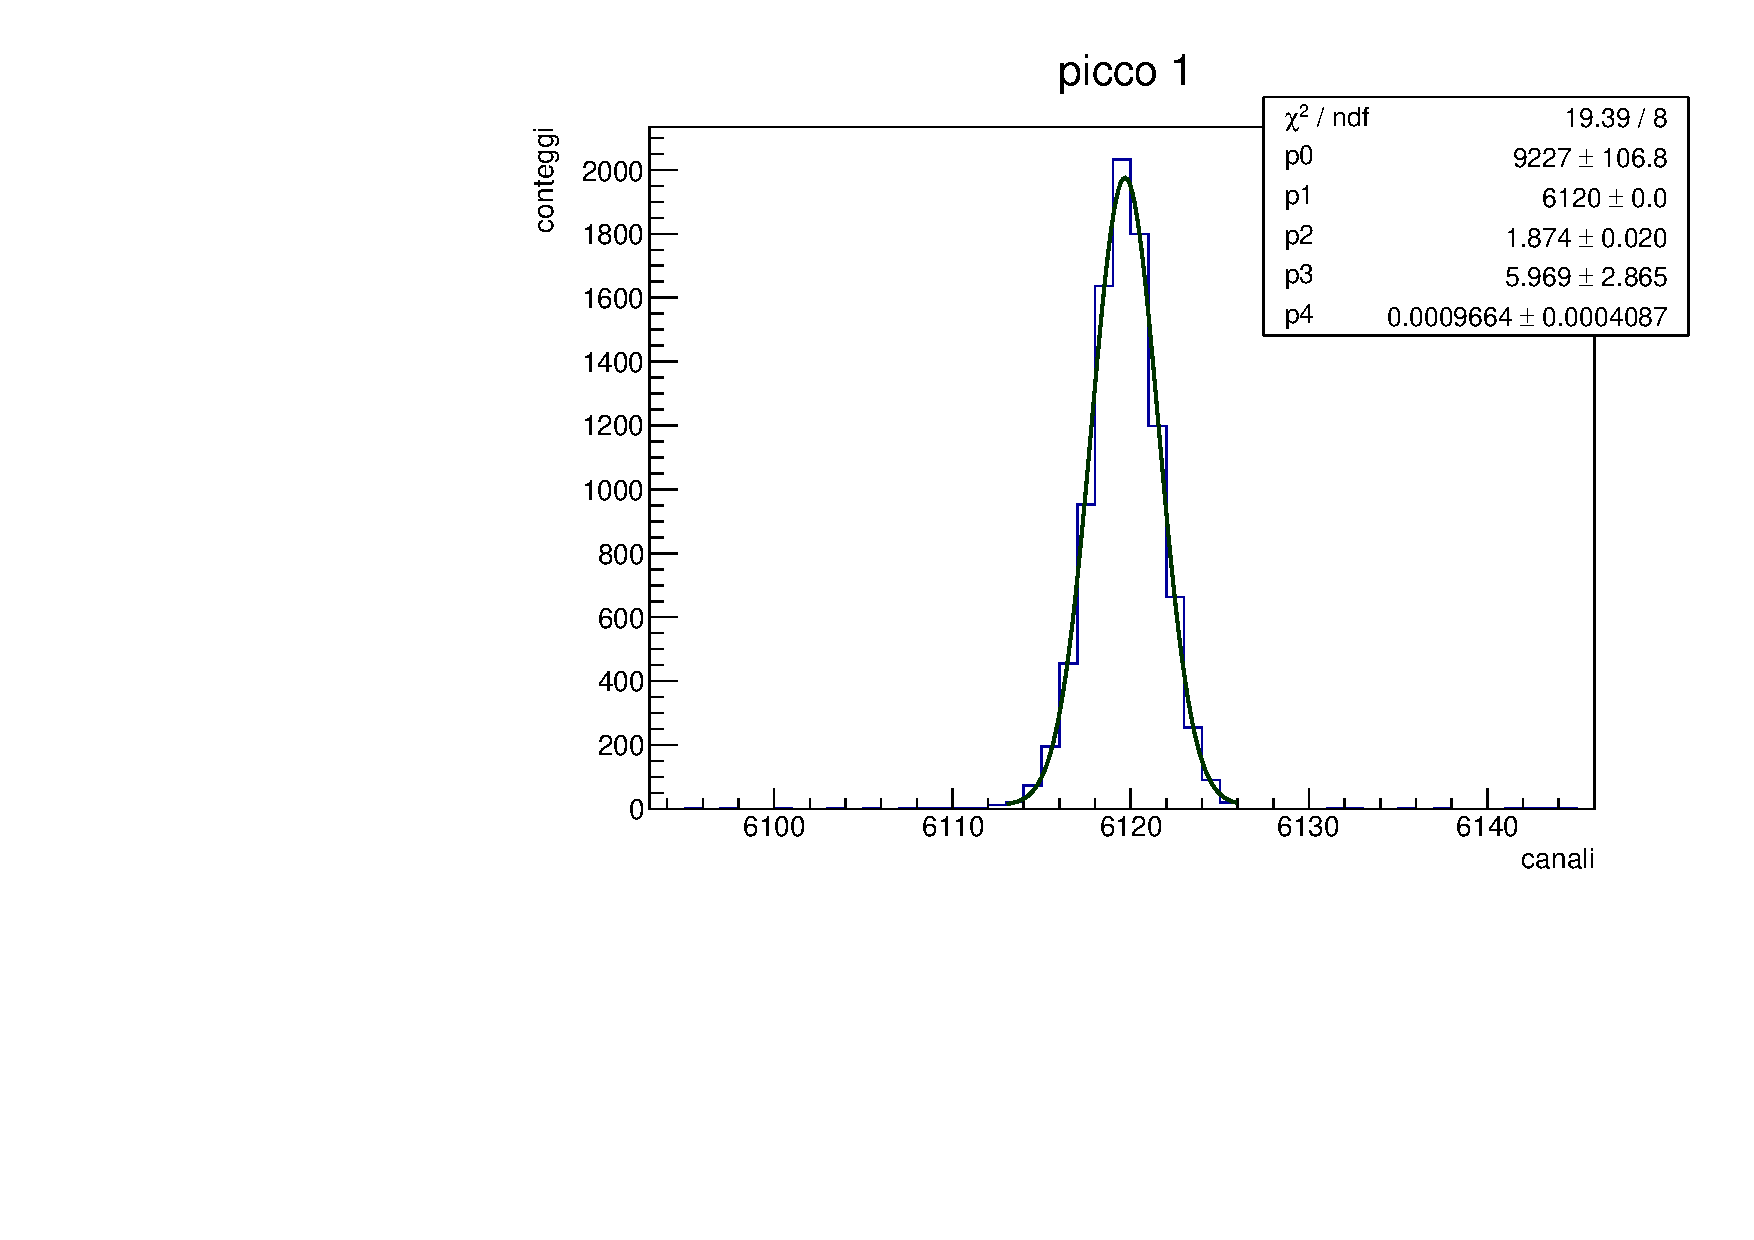
\includegraphics[width=3.4cm]{grafici/picco_pulser_germanio_1.pdf}                        
                \end{figure}

                \begin{table}[h!]
                    \centering
                    \caption{risultati fit pulser}
                    \label{tab:fit_picco_pulser_germanio}
                    $
                    \begin{array}{ccccccccccc}
	\toprule
	(canali) & N & \delta N & X & \delta X & \sigma & \delta\sigma & FWHM & \delta FWHM & \chi^2 & NDF \\
	\midrule
	\text{picco 1} & 9227 & 107 &  6119.681 & 0.020  &  1.874 & 0.020  &  4.413 & 0.048  & 19.39 & 8 \\
	\bottomrule
\end{array}
                    $
                \end{table}

            Infine, la $FWHM$ del pulser convertita in energia è:
            \begin{equation*}
                \boxed{FWHM=(1.434\pm0.016)\:\si{\kilo\electronvolt}}
            \end{equation*}

    \section{L'efficienza}
        L'andamento dell'efficienza assoluta rispetto all'energia può essere studiato mediante un best fit rispetto alla formula \eqref{for:fit_efficienza}. Infatti, bisogna calcolare l'attività delle due sorgenti al tempo dell'esperimento, nota la stessa al momento dell'acquisto, e per farlo basterà applicare \eqref{for:attività}.

        Per il fit, invece, basterà applicare un solo codice in grado di calcolare $\epsilon$ per tutti i picchi di interesse.

        \subsection*{Il funzionamento del codice}
            La macro \textit{fit\_efficienza.cpp} è in grado di eseguire il best fit caratteristico dell'efficienza assoluta calcolandone i suoi valori al variare dell'energia, e di calcolare i residui per ciascuna per verificare il grado a cui arrestarsi.

            \textbf{Input}: file di testo con tempi di acquisizione $T$ (live time), attività $A$, $B.R.$, energie tabulate, numero di conteggi e corrispondente incertezza per ciascun picco.

            \textbf{Output}: valori dell'efficienza al variare dell'energia e dei parametri del best fit in file di testo e plot del fit caratteristico e dell'andamento dei residui in pdf.

        \subsection*{I risultati ottenuti}
            La tabella \ref{tab:attività} mostra, per le due sorgenti, il tempo $\Delta t$ trascorso dall'acquisto all'uso dei campioni e la loro attività $A$ al momento dell'esperimento, calcolata mediante la \eqref{for:attività}.
                \begin{table}[h!]
                    \centering
                    \caption{attività sorgenti}
                    \label{tab:attività}
                    $
                    \begin{array}{cccccc}
                        \toprule
                        \text{sorgente}       & \Delta t\:\si{(\second)} & A\:\si{(\kilo\becquerel)} \\
                        \midrule
                        \text{Europio-152}&8.71\cdot10^{8}&8.99\\
                        \text{Cobalto-60}&8.15\cdot10^{8}&1.24\\
                        \text{Cobalto-60 (alto rateo)}&8.15\cdot10^{8}&14.39\\
                        \bottomrule
                    \end{array}
                    $
                \end{table}
                
            La tabella \ref{tab:efficienze} mostra, per l'europio-152 e per il cobalto-60, le efficienze in percentuali di ciascun picco con la corrispondente incertezza.
                \begin{table}[h!]
                    \centering
                    \caption{efficienze}
                    \label{tab:efficienze}
                    \subtable[Europio-152]
                        {
                            $
                            \begin{array}{ccc}
	\toprule
	\% & \epsilon & \delta\epsilon \\
	\midrule
	\text{picco 1} & 4.28 & 0.22  \\
	\text{picco 2} & 3.29 & 0.17  \\
	\text{picco 3} & 2.81 & 0.14  \\
	\text{picco 4} & 1.83 & 0.12  \\
	\text{picco 5} & 1.84 & 0.12  \\
	\text{picco 6} & 0.987 & 0.054  \\
	\text{picco 7} & 0.793 & 0.057  \\
	\text{picco 8} & 0.845 & 0.046  \\
	\text{picco 9} & 0.639 & 0.051  \\
	\text{picco 10} & 0.719 & 0.047  \\
	\text{picco 11} & 0.599 & 0.033  \\
	\bottomrule
\end{array}

                            $
                        }
                    \subtable[Cobalto-60]
                        {
                            $
                            \begin{array}{ccc}
	\toprule
	\% & \epsilon & \delta\epsilon \\
	\midrule
	\text{picco 1}& 0.422 & 0.023  \\
	\text{picco 2}& 0.361 & 0.020  \\
	\bottomrule
\end{array}

                            $
                        }
                    \subtable[Cobalto-60 (alto rateo)]
                        {
                            $
                            \begin{array}{ccc}
	\toprule
	\% & \epsilon & \delta\epsilon \\
	\midrule
	\text{picco 1}& 0.01329 & 0.00068  \\
	\text{picco 2}& 0.01212 & 0.00062  \\
	\bottomrule
\end{array}

                            $
                        }
                \end{table}

                La tabella \ref{tab:fit_efficienza} e la figura \ref{fig:fit_efficienza} mostrano i risultati del fit caratteristico delle efficienze rispetto all'energia, come nella formula \eqref{for:efficienza}.
                
                \begin{table}[h!]
                    \centering
                    \caption{fit caratteristico efficienza}
                    \label{tab:fit_efficienza}
                    $
                    \begin{array}{cccccccc}
	\toprule
	\rho_0 &  \delta\rho_0 & \rho_1 &  \delta\rho_1 & \rho_2 &  \delta\rho_2 & \chi^2 & NDF \\
	\midrule
	 -9.66 & 0.13  &  2.920 & 0.038  &  -0.3248 & 0.0035  & 101.27 & 10 \\
	\bottomrule
\end{array}

                    $
                \end{table}

                \begin{figure}[h!]
                    \centering
                    \caption{fit efficienze con energie tabulate ($N=2$)}
                    \label{fig:fit_efficienza}
                    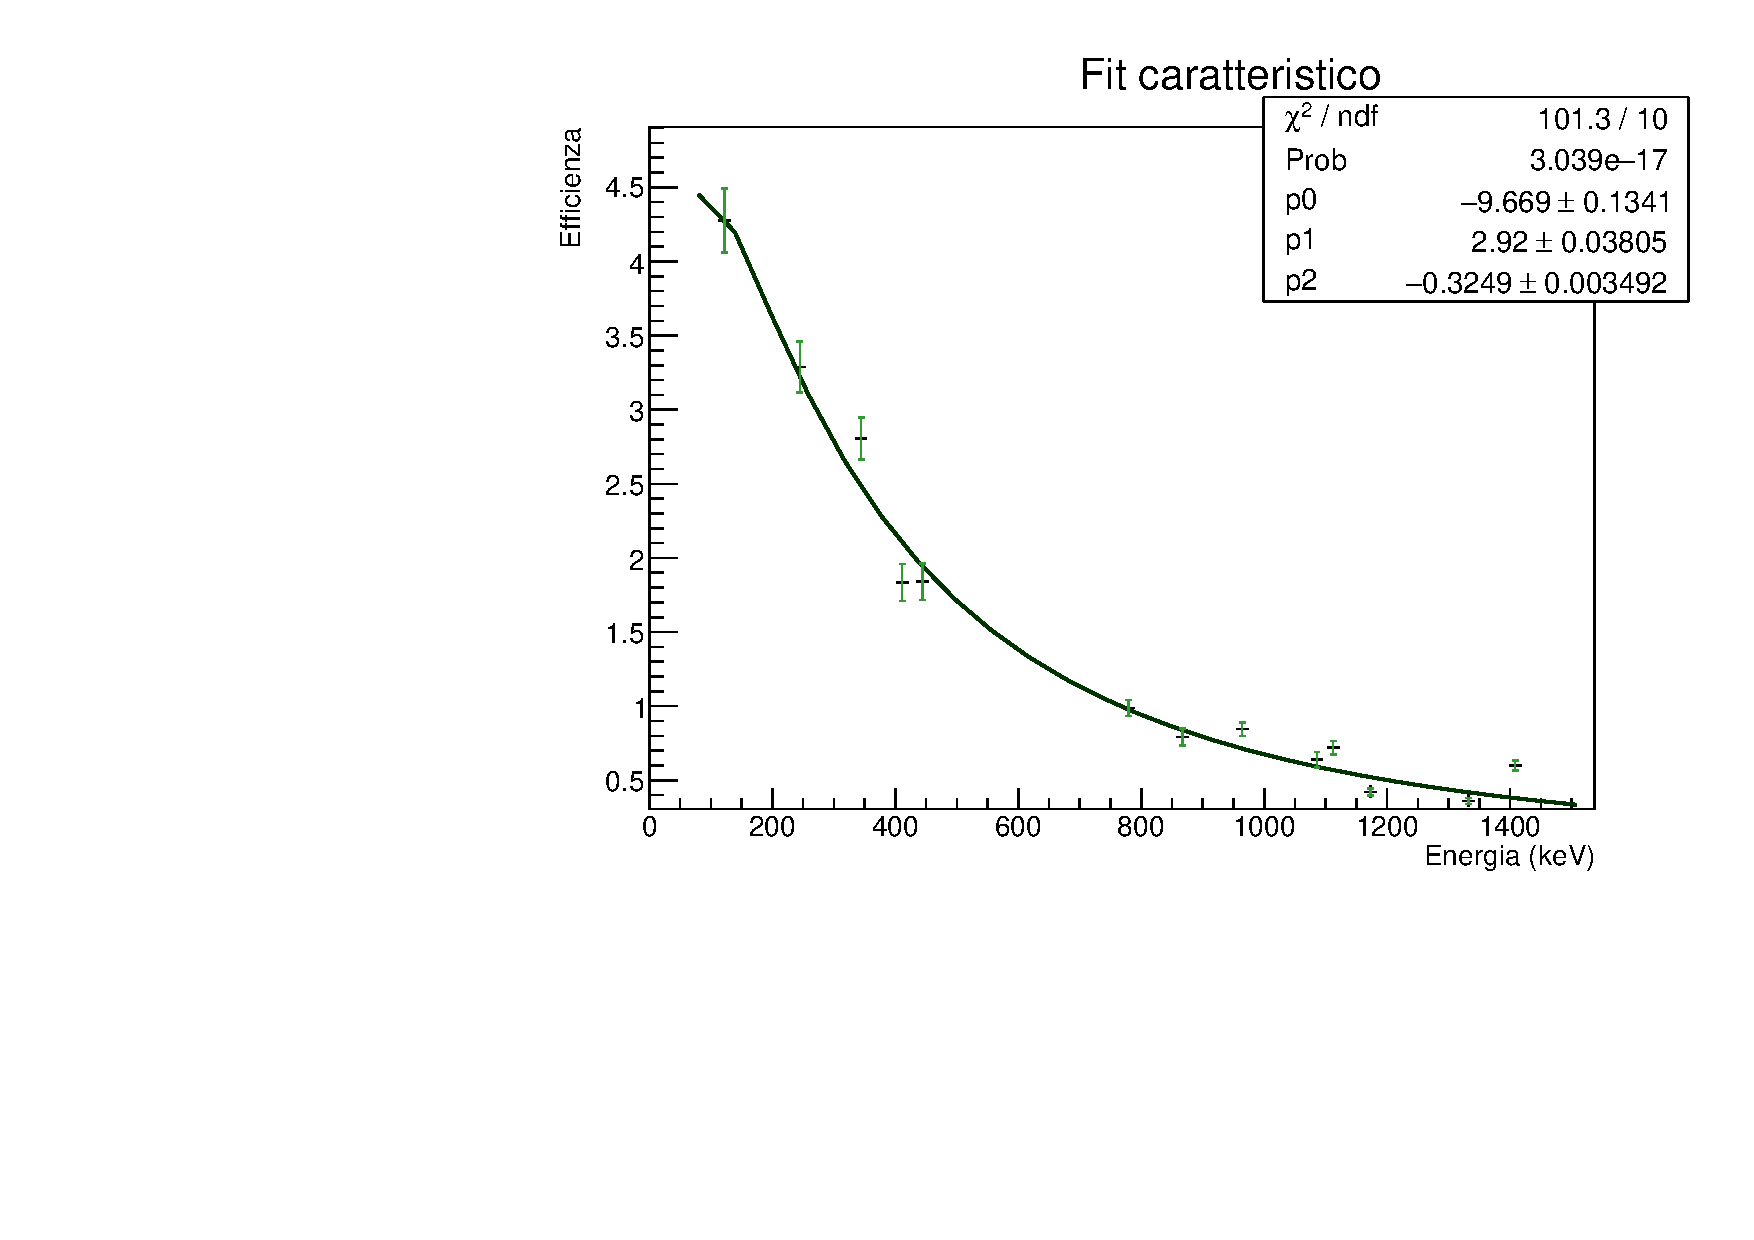
\includegraphics[width=10cm]{grafici/fit_efficienza_2.pdf}
                \end{figure}

                Infine, la figura \ref{fig:fit_efficienza_residui} mostra l'andamento dei residui rispetto all'energia tabulata per $N=0,1,2$ nella sommatoria della funzione di fit, confermando che il grado minimo per cui il loro andamento è casuale è proprio $N=2$, mentre per $N=0,1$ sono evidentemente crescenti.
  
                \begin{figure}[h!]
                \centering
                \caption{residui fit efficienza}
                \label{fig:fit_efficienza_residui}
                \subfigure[$N=0$]
                    {
                        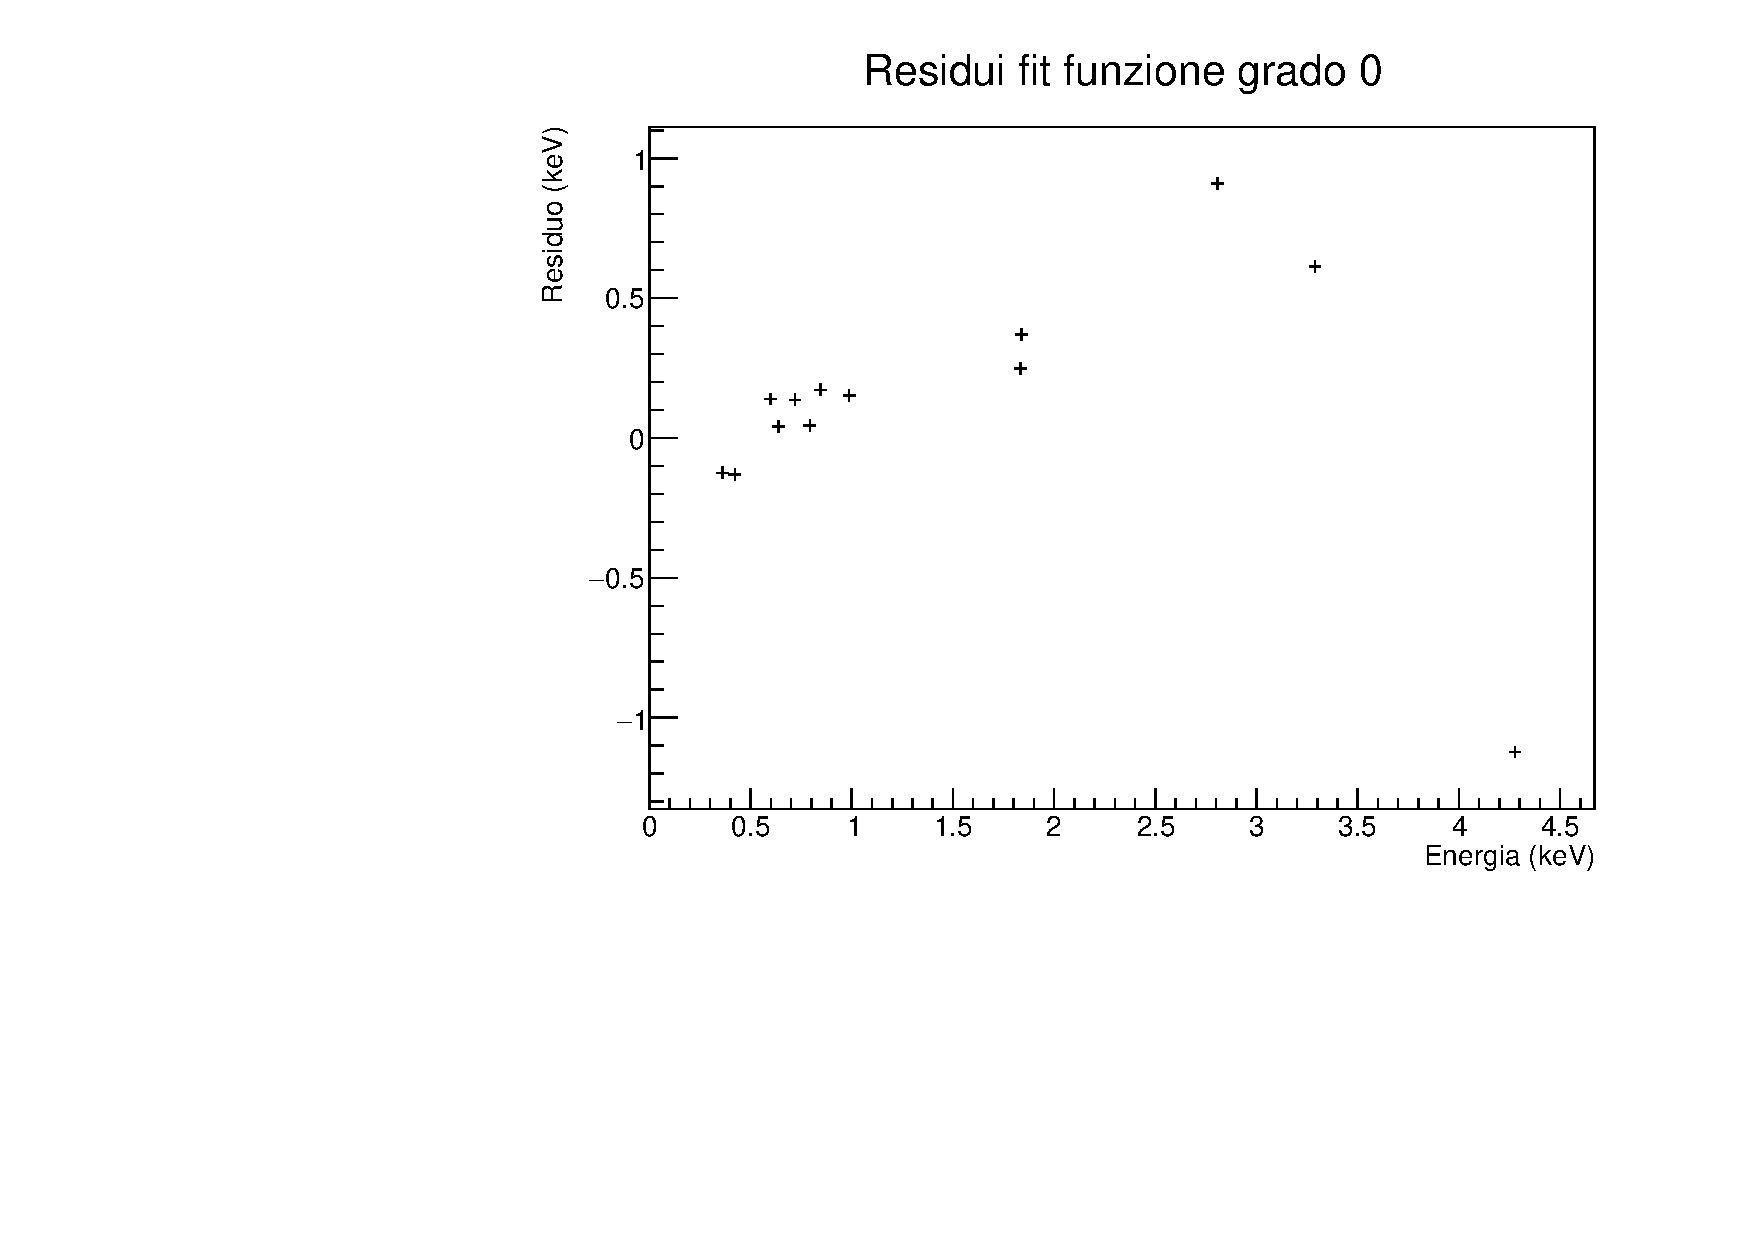
\includegraphics[width=4.5cm]{grafici/fit_efficienza_residui_0.pdf}
                    }
                \subfigure[$N=1$]
                    {
                        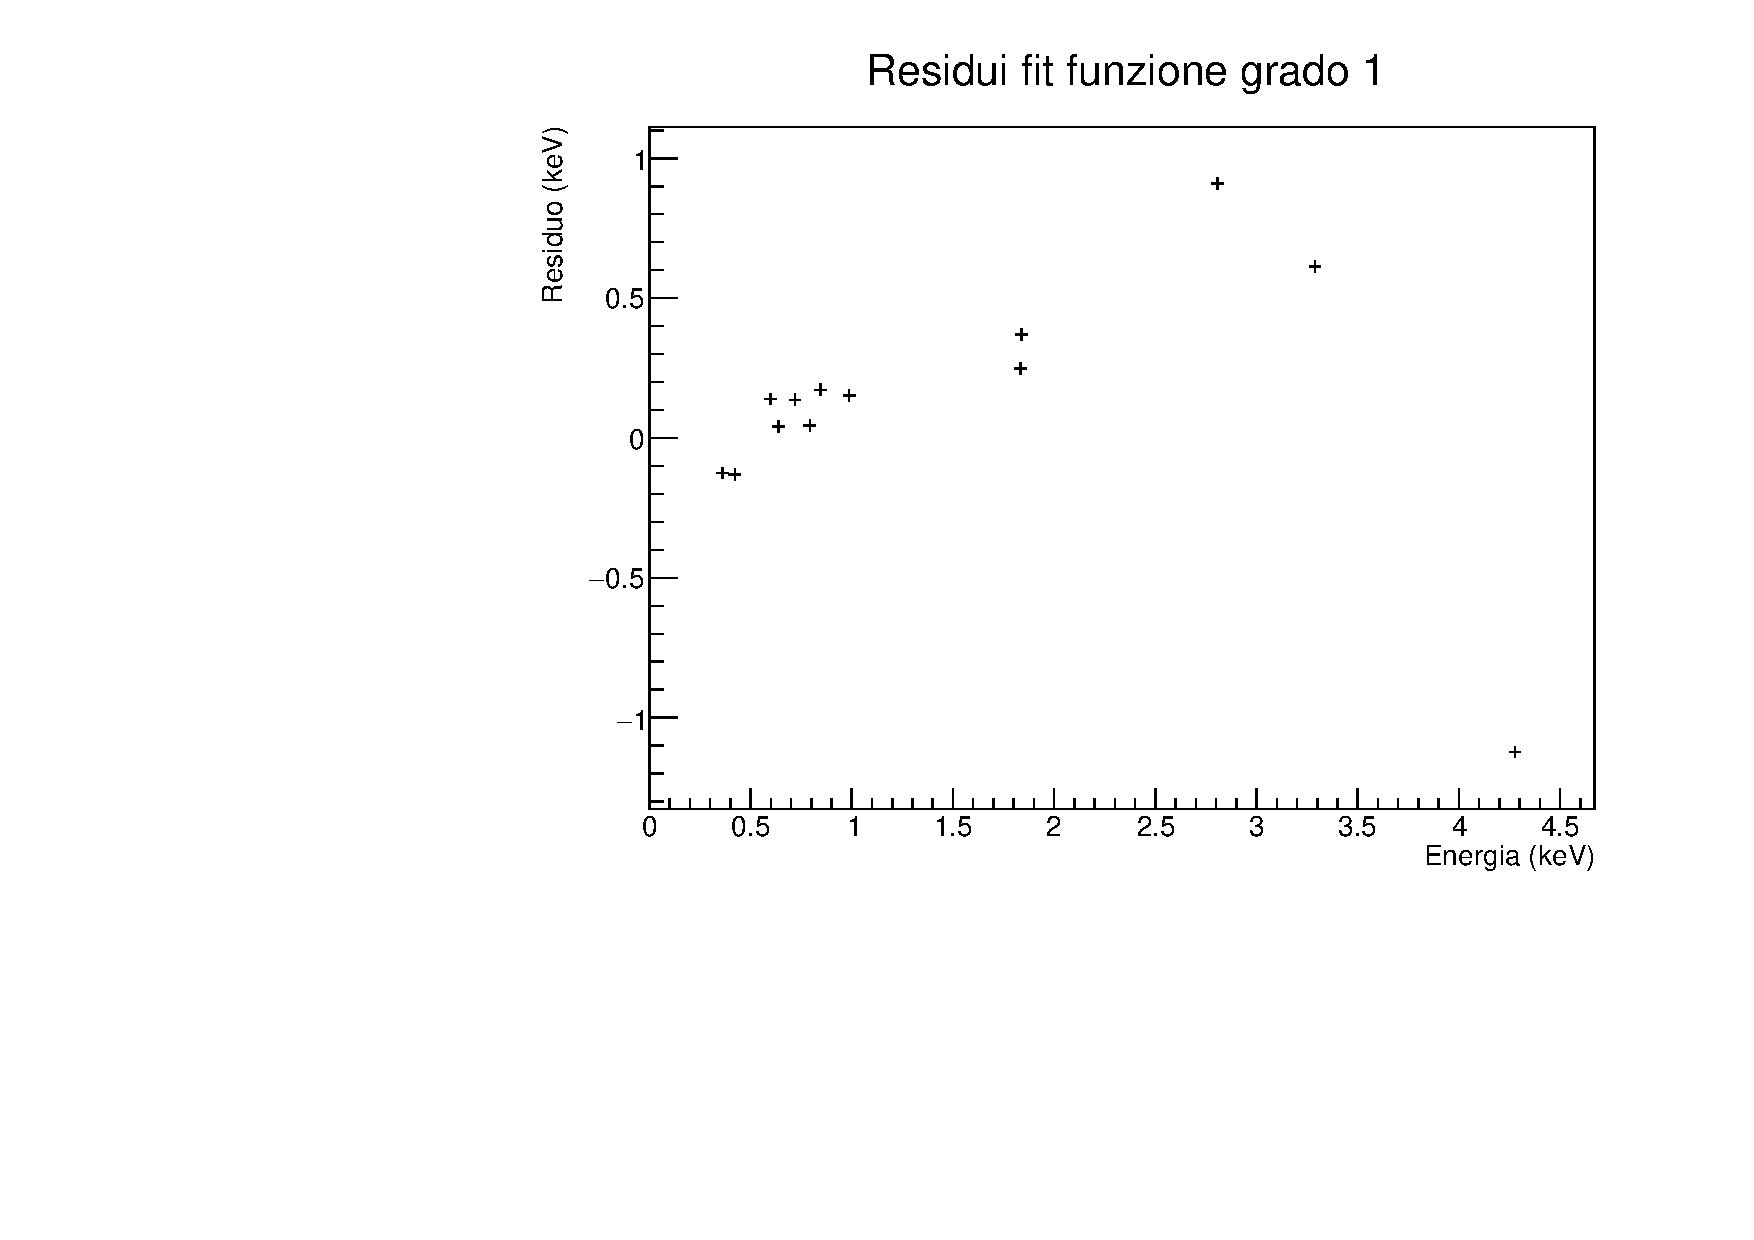
\includegraphics[width=4.5cm]{grafici/fit_efficienza_residui_1.pdf}
                    }
                \subfigure[$N=2$]
                    {
                        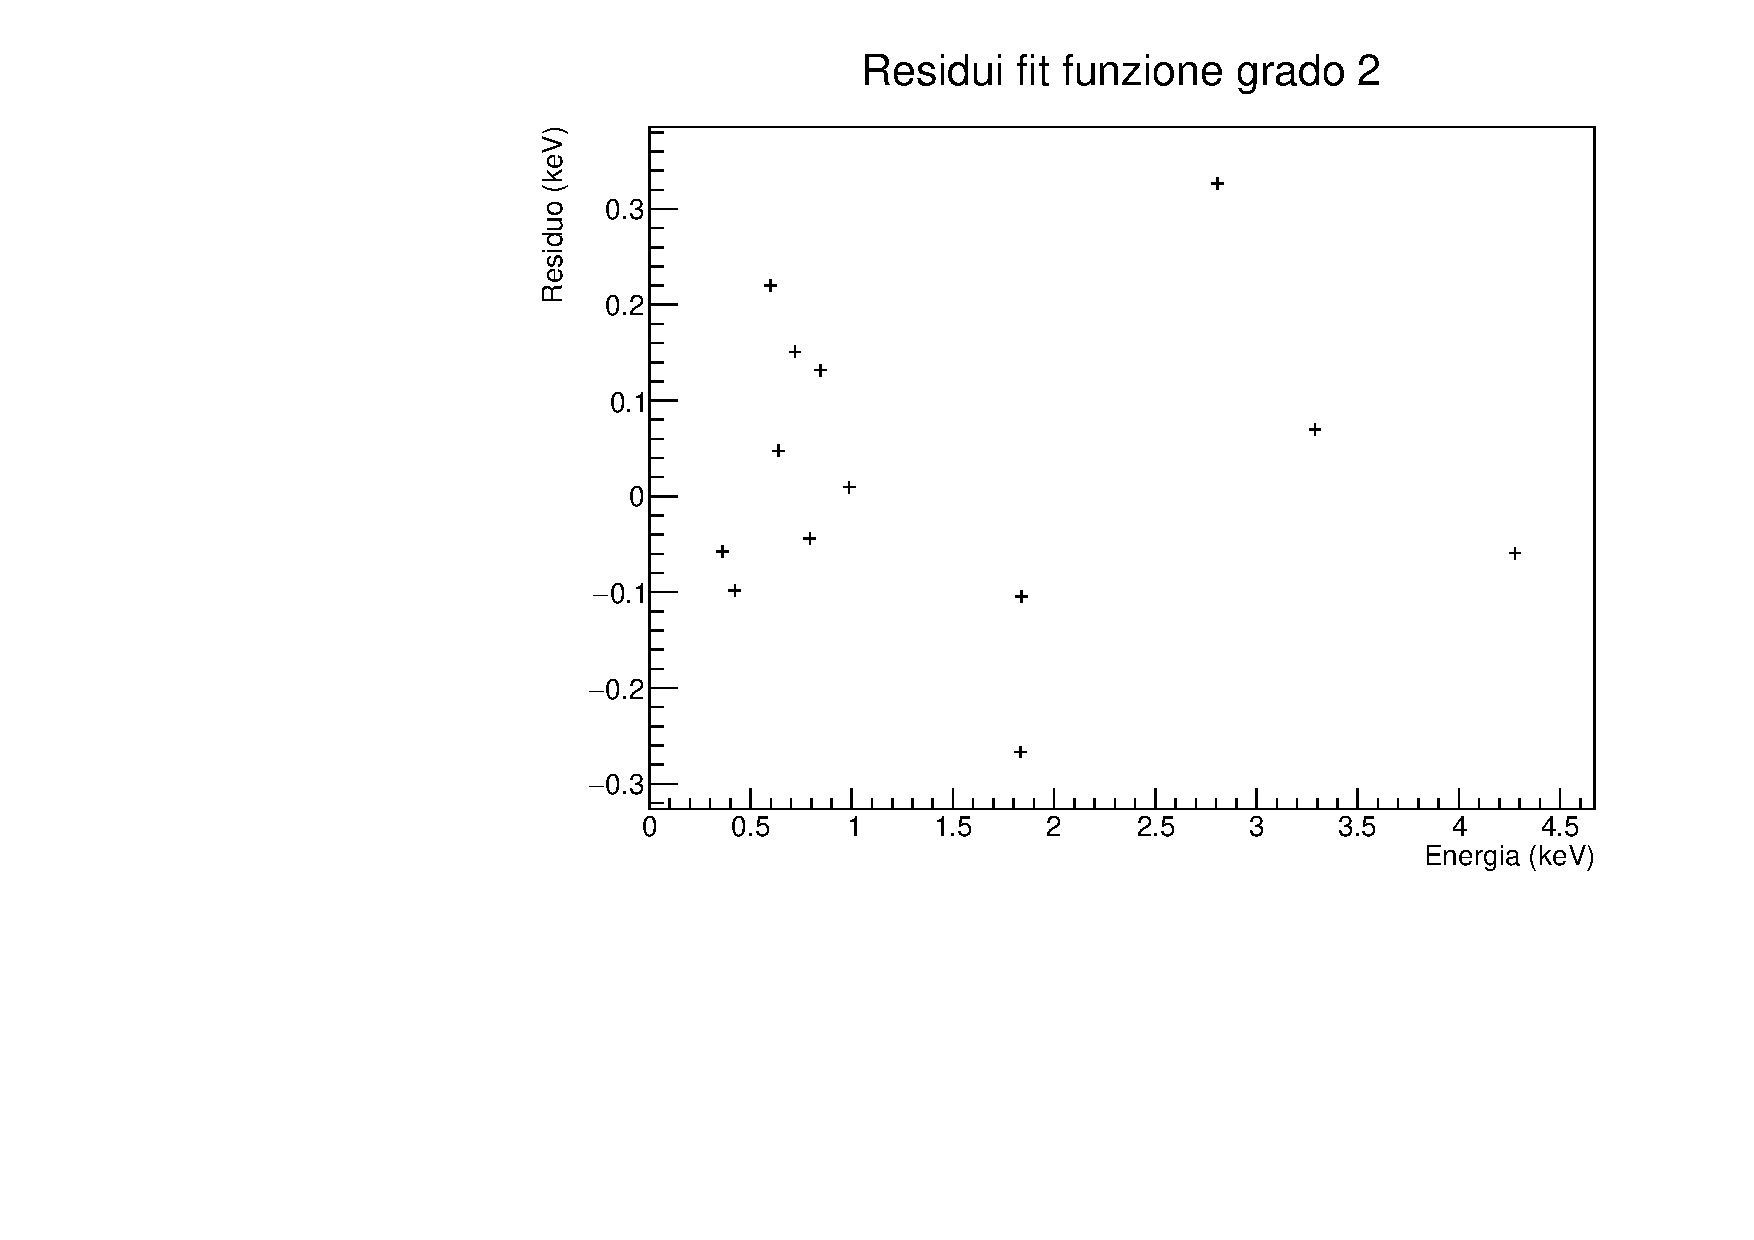
\includegraphics[width=4.5cm]{grafici/fit_efficienza_residui_2.pdf}
                    }
            \end{figure}

    \section{La sorgente incognita}
        Sempre con i codici precedenti, noti i parametri di calibrazione, è possibile studiare una sorgente incognita assegnando dei valori corrispondenti in energia ai risultati dei fit gaussiani dello spettro in canali. A tal proposito, con le stesse note operative precedenti, è possibile far girare il codice più volte fino a quando non si sono individuati più picchi possibili.
        
        \subsection*{I risultati ottenuti}   
            La figura \ref{fig:spettro_incognita_germanio} mostra lo spettro della sorgente incognita con e senza il fondo.
            \begin{figure}[h!]
                \centering
                \caption{spettro sorgente incognita}
                \label{fig:spettro_incognita_germanio}
                \subfigure[sorgente incognita con fondo]
                    {
                        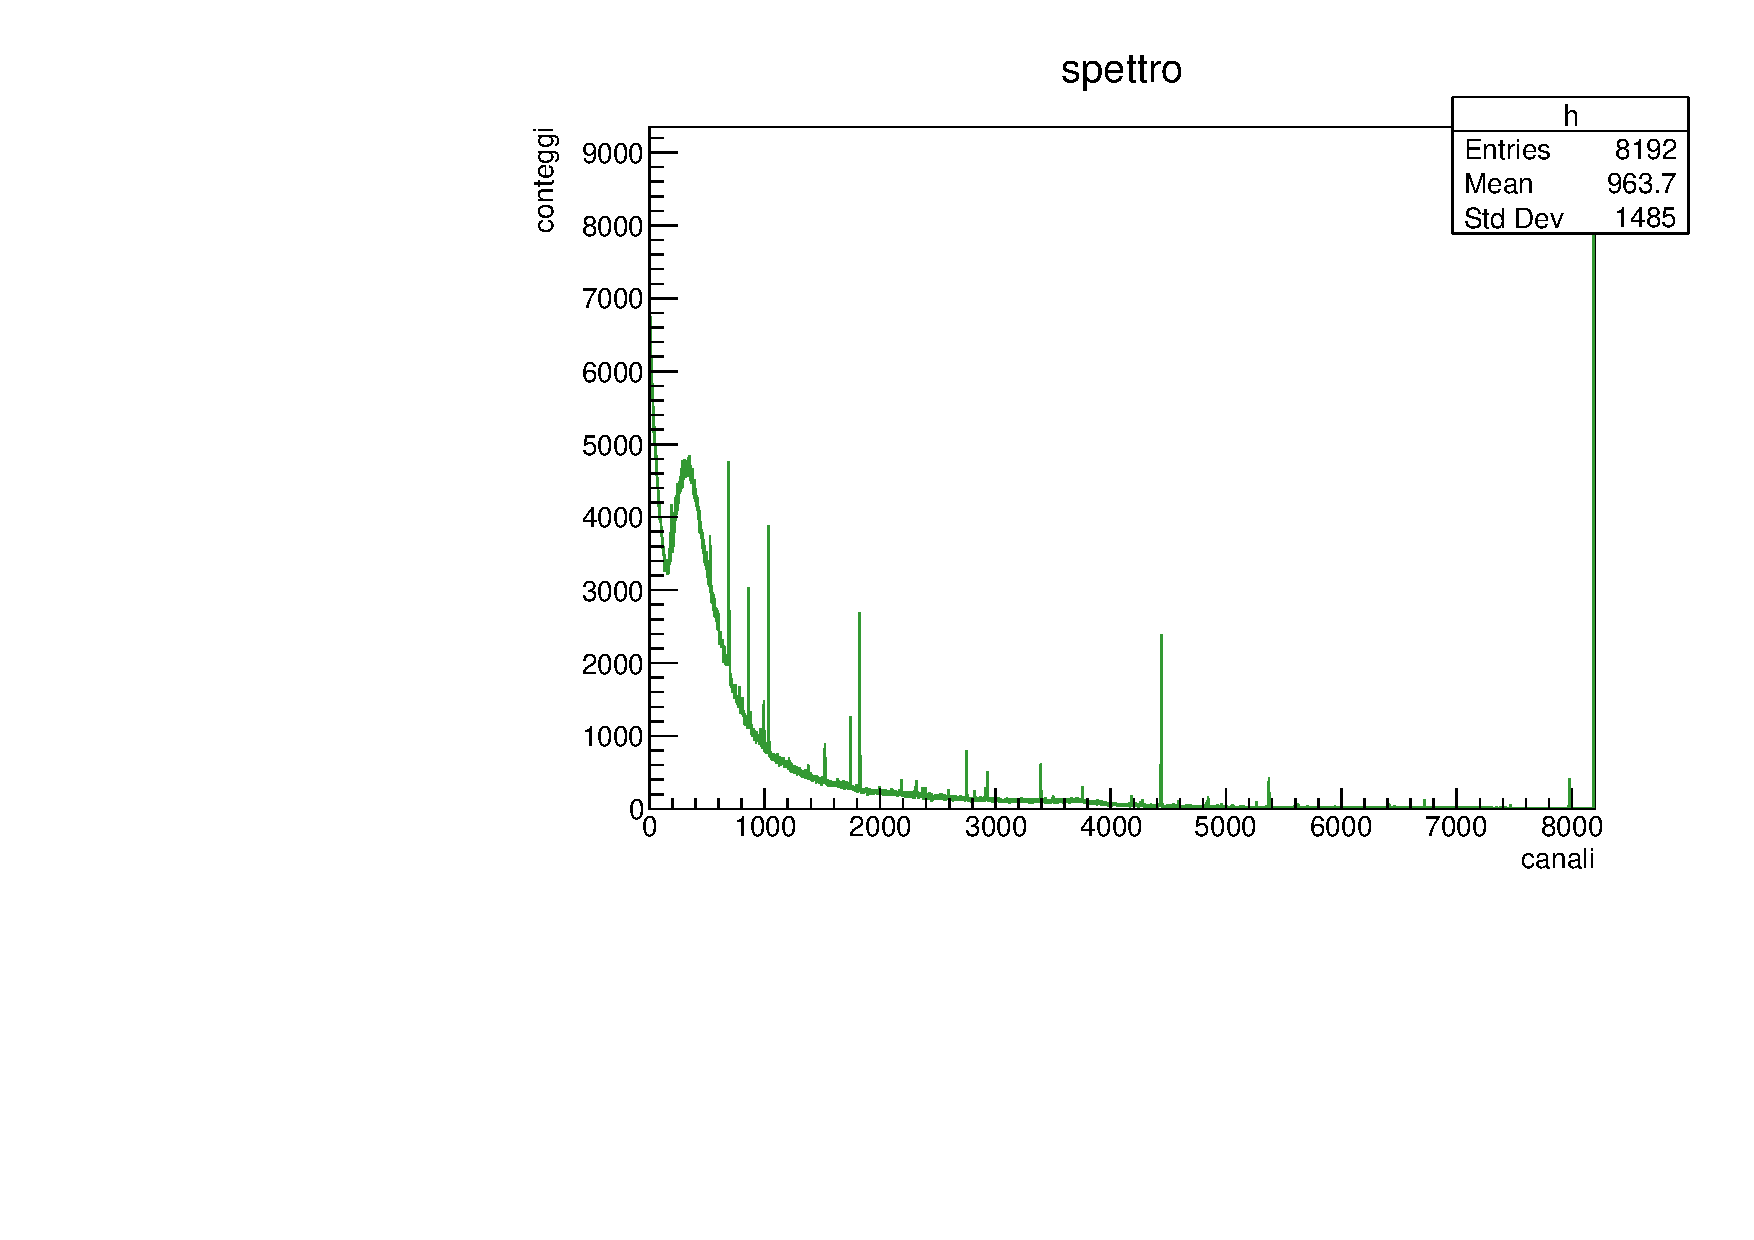
\includegraphics[width=5cm]{grafici/spettro_incognita_germanio_con_fondo.pdf}
                    }
                \subfigure[sorgente incognita senza fondo]
                    {
                        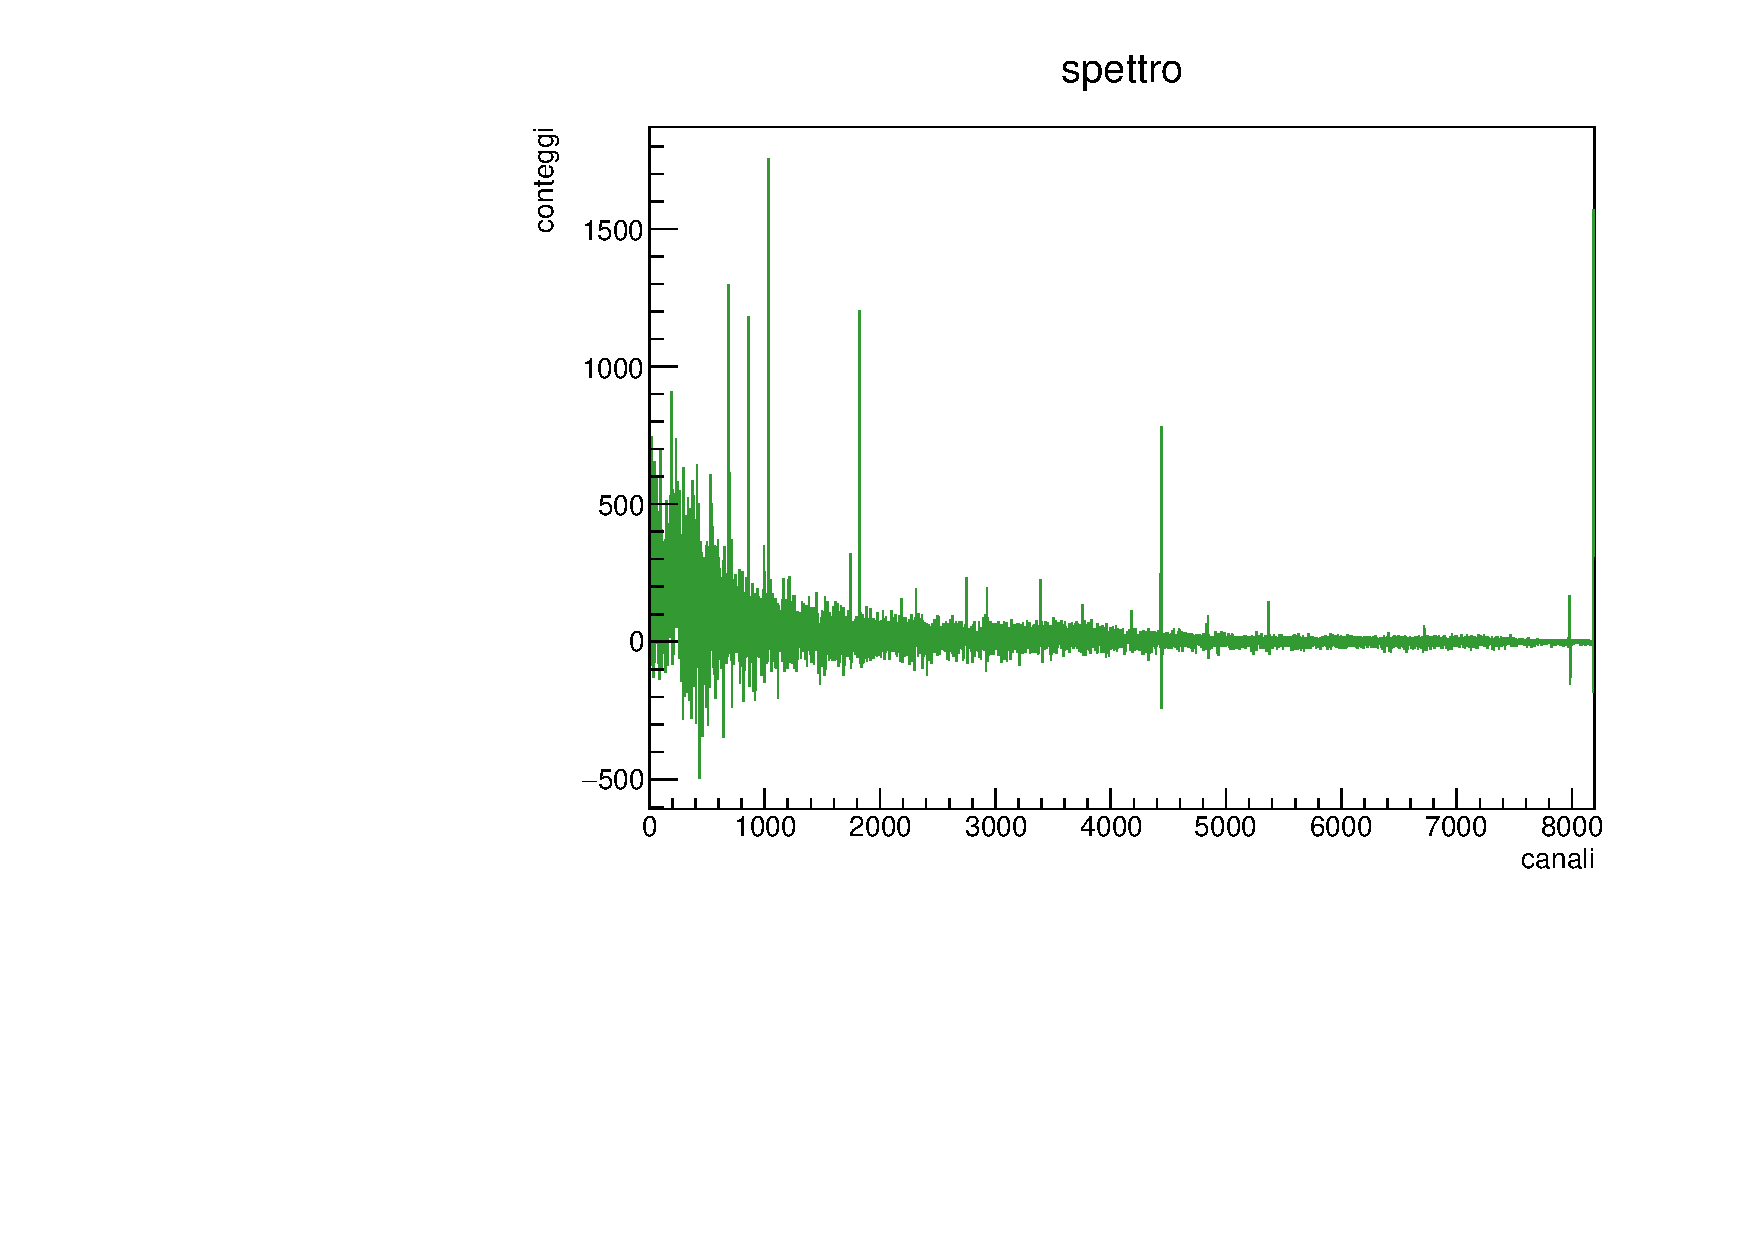
\includegraphics[width=5cm]{grafici/spettro_incognita_germanio_senza_fondo.pdf}
                    }
            \end{figure}

            Le figure \ref{fig:picchi_incognita_germanio_1} e \ref{fig:picchi_incognita_germanio_2} e la tabella \ref{tab:fit_picchi_incognita_germanio} mostrano i risultati dei fit dei singoli picchi individuati.
            \begin{figure}[h!]
                \centering
                \caption{picchi sorgente incognita con fit}
                \label{fig:picchi_incognita_germanio_1}
                \subfigure[picco 1]
                    {
                        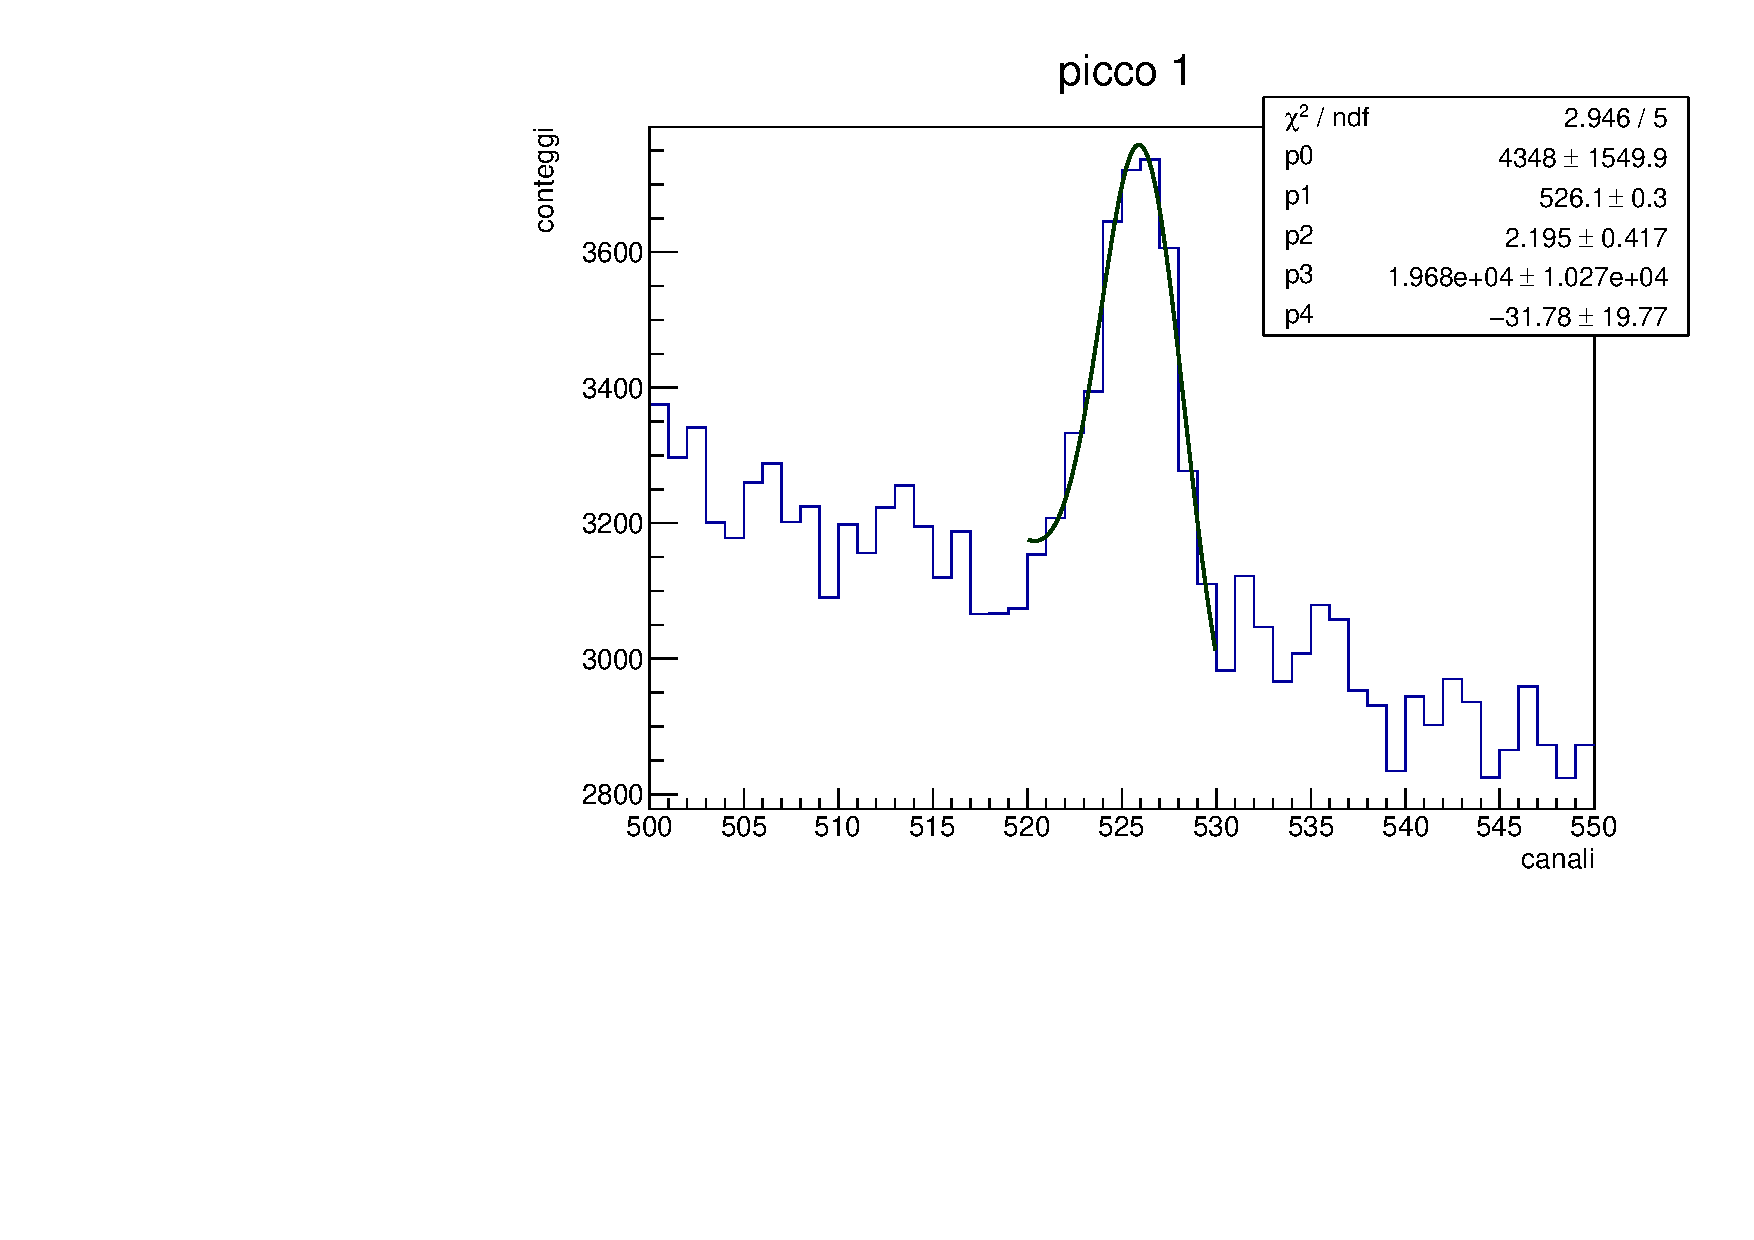
\includegraphics[width=2.2cm]{grafici/picco_incognita_germanio_1.pdf}
                    }
                \subfigure[picco 2]
                    {
                        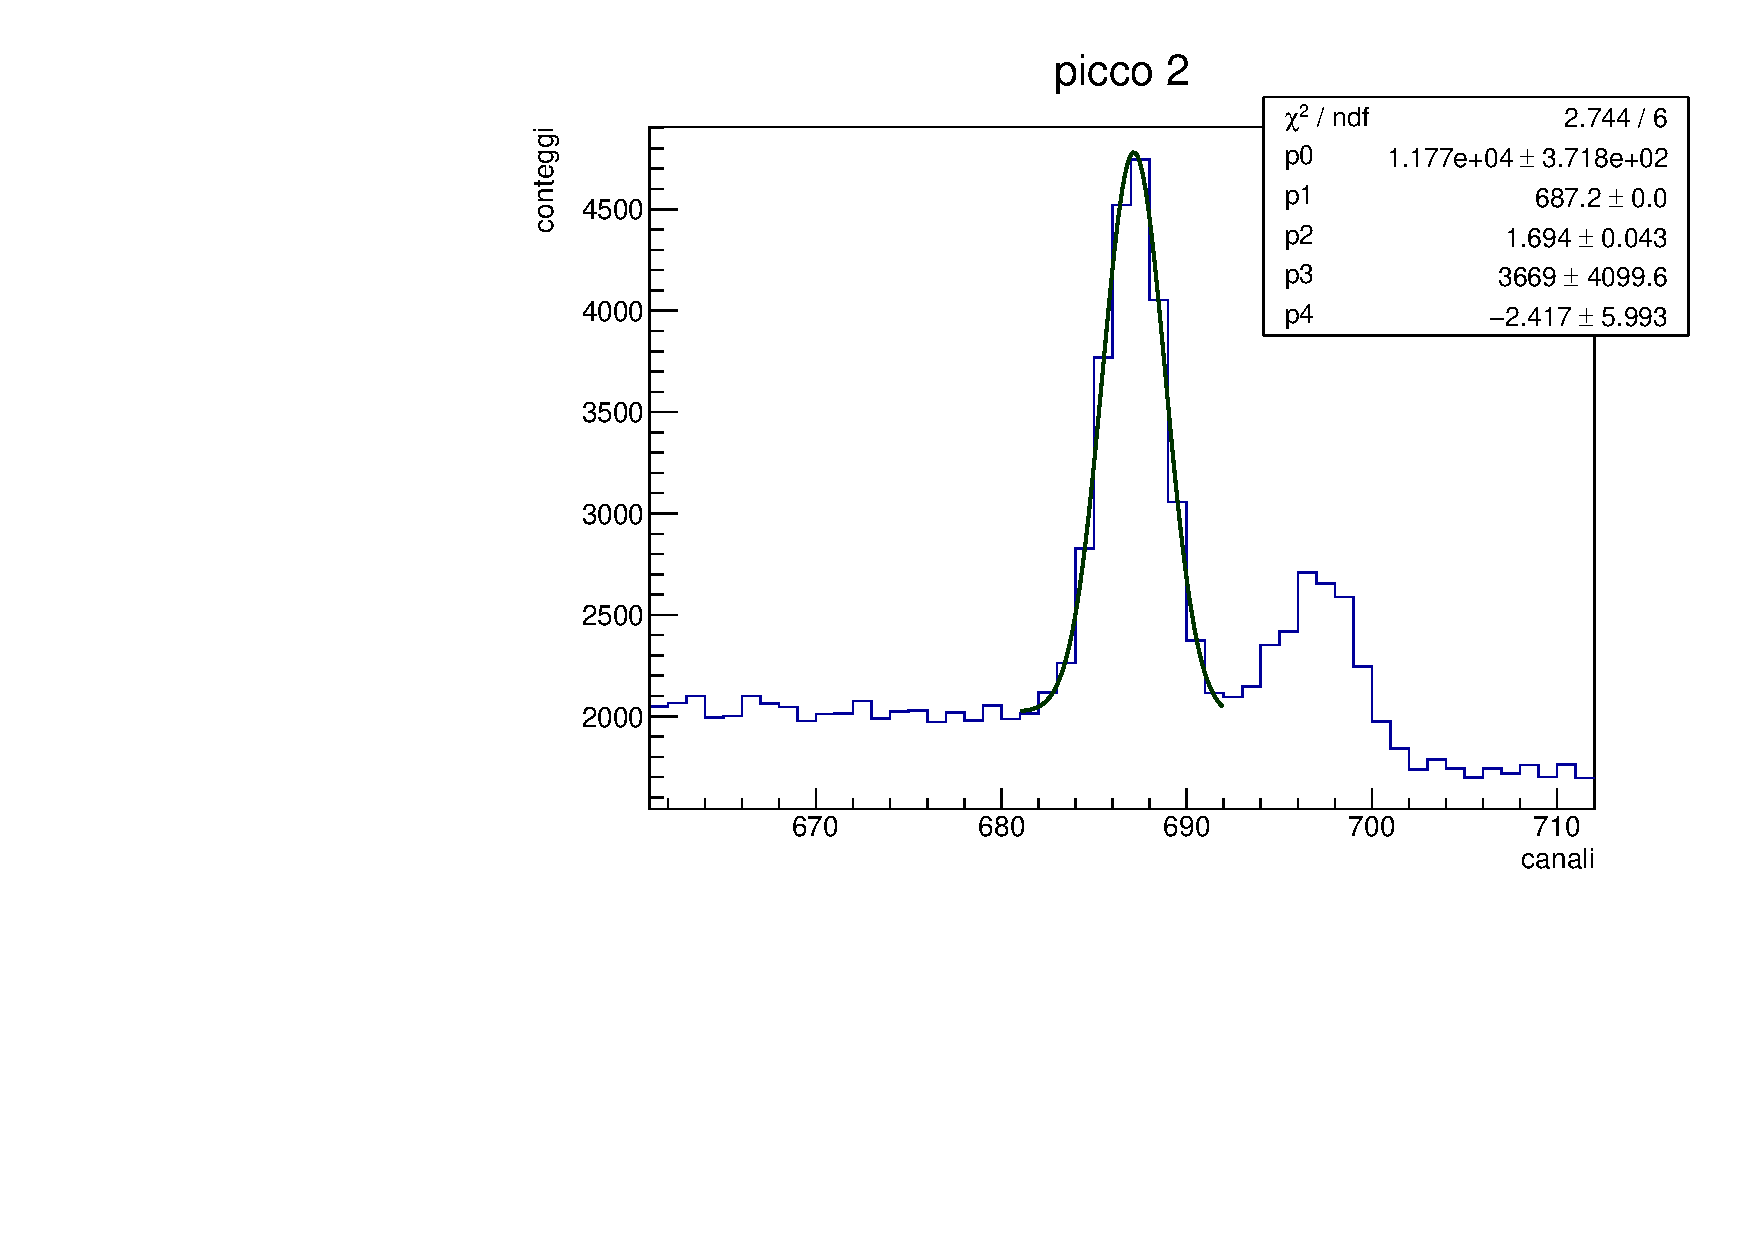
\includegraphics[width=2.2cm]{grafici/picco_incognita_germanio_2.pdf}
                    }
                \subfigure[picco 3]
                    {
                        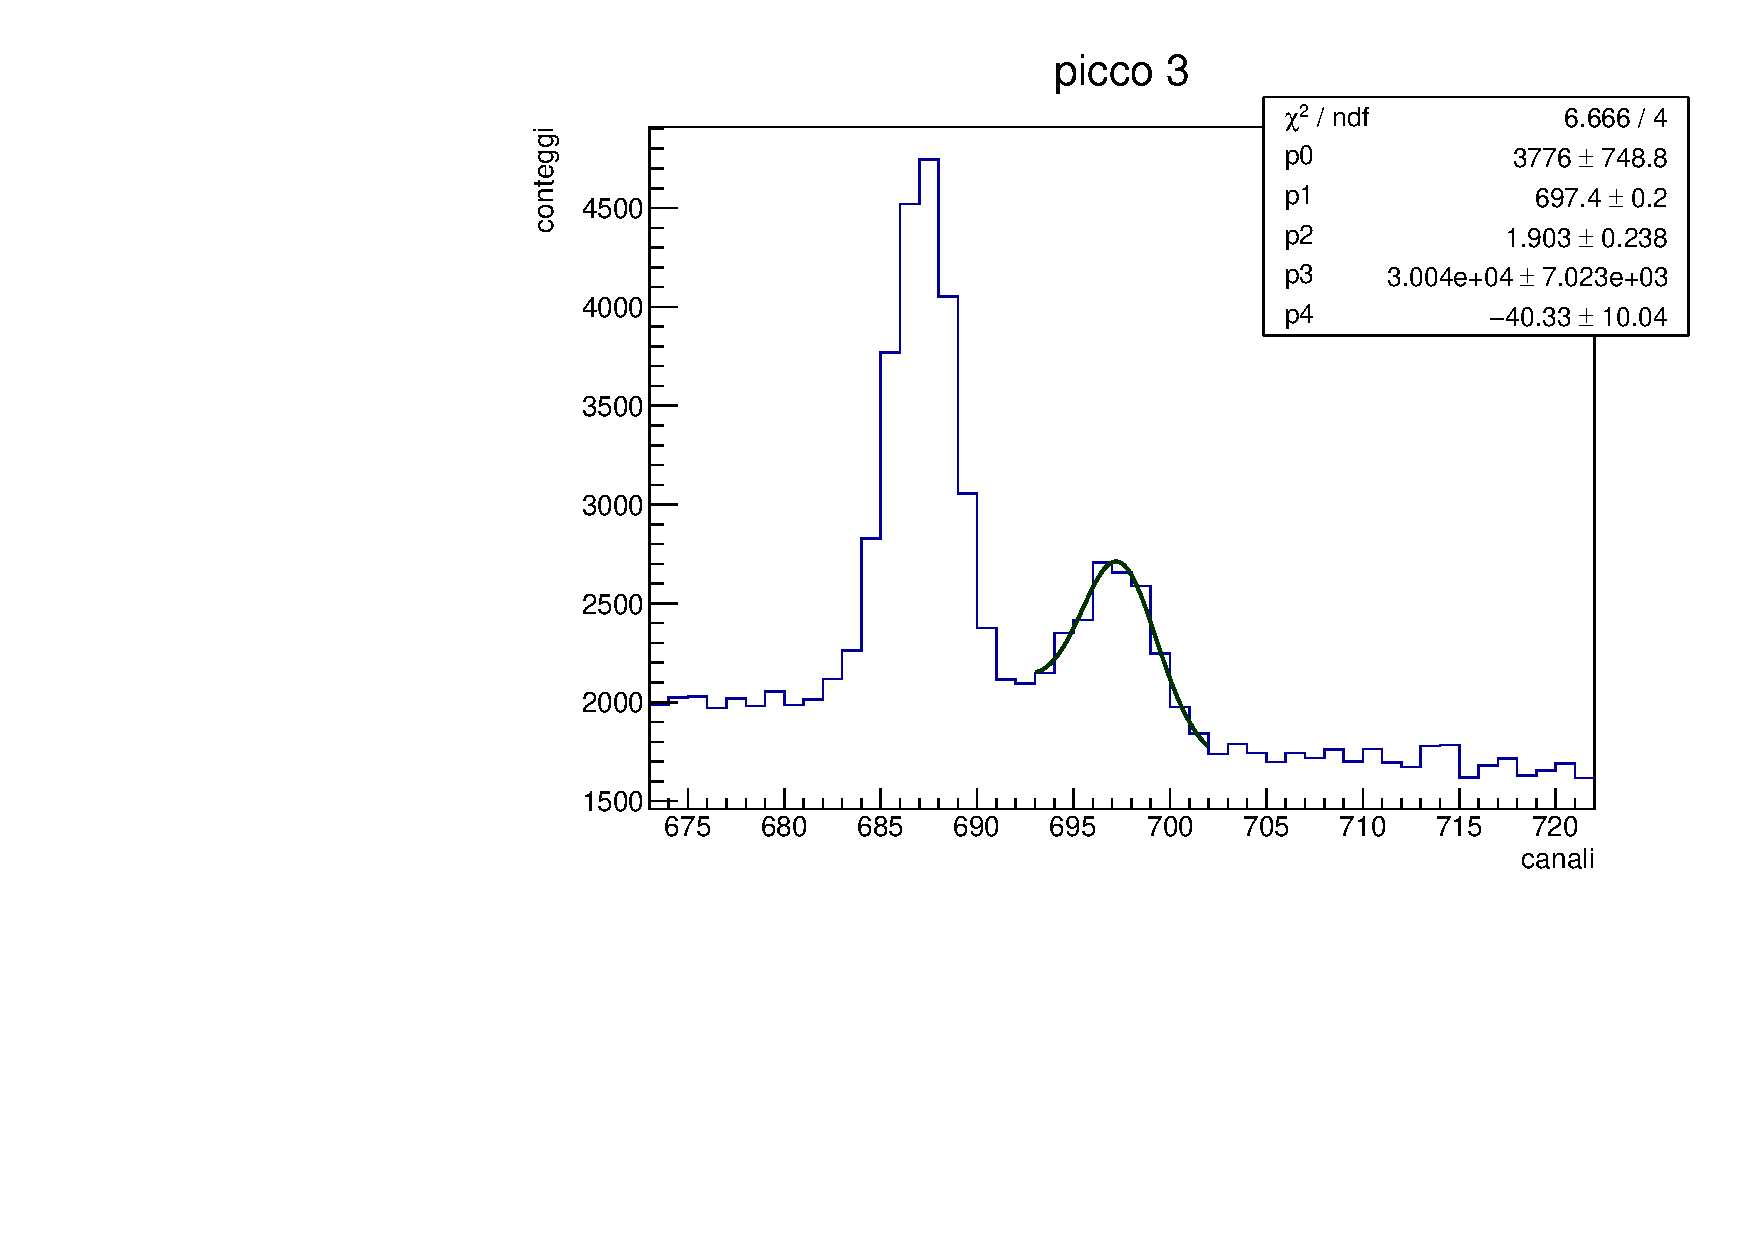
\includegraphics[width=2.2cm]{grafici/picco_incognita_germanio_3.pdf}
                    }
                \subfigure[picco 4]
                    {
                        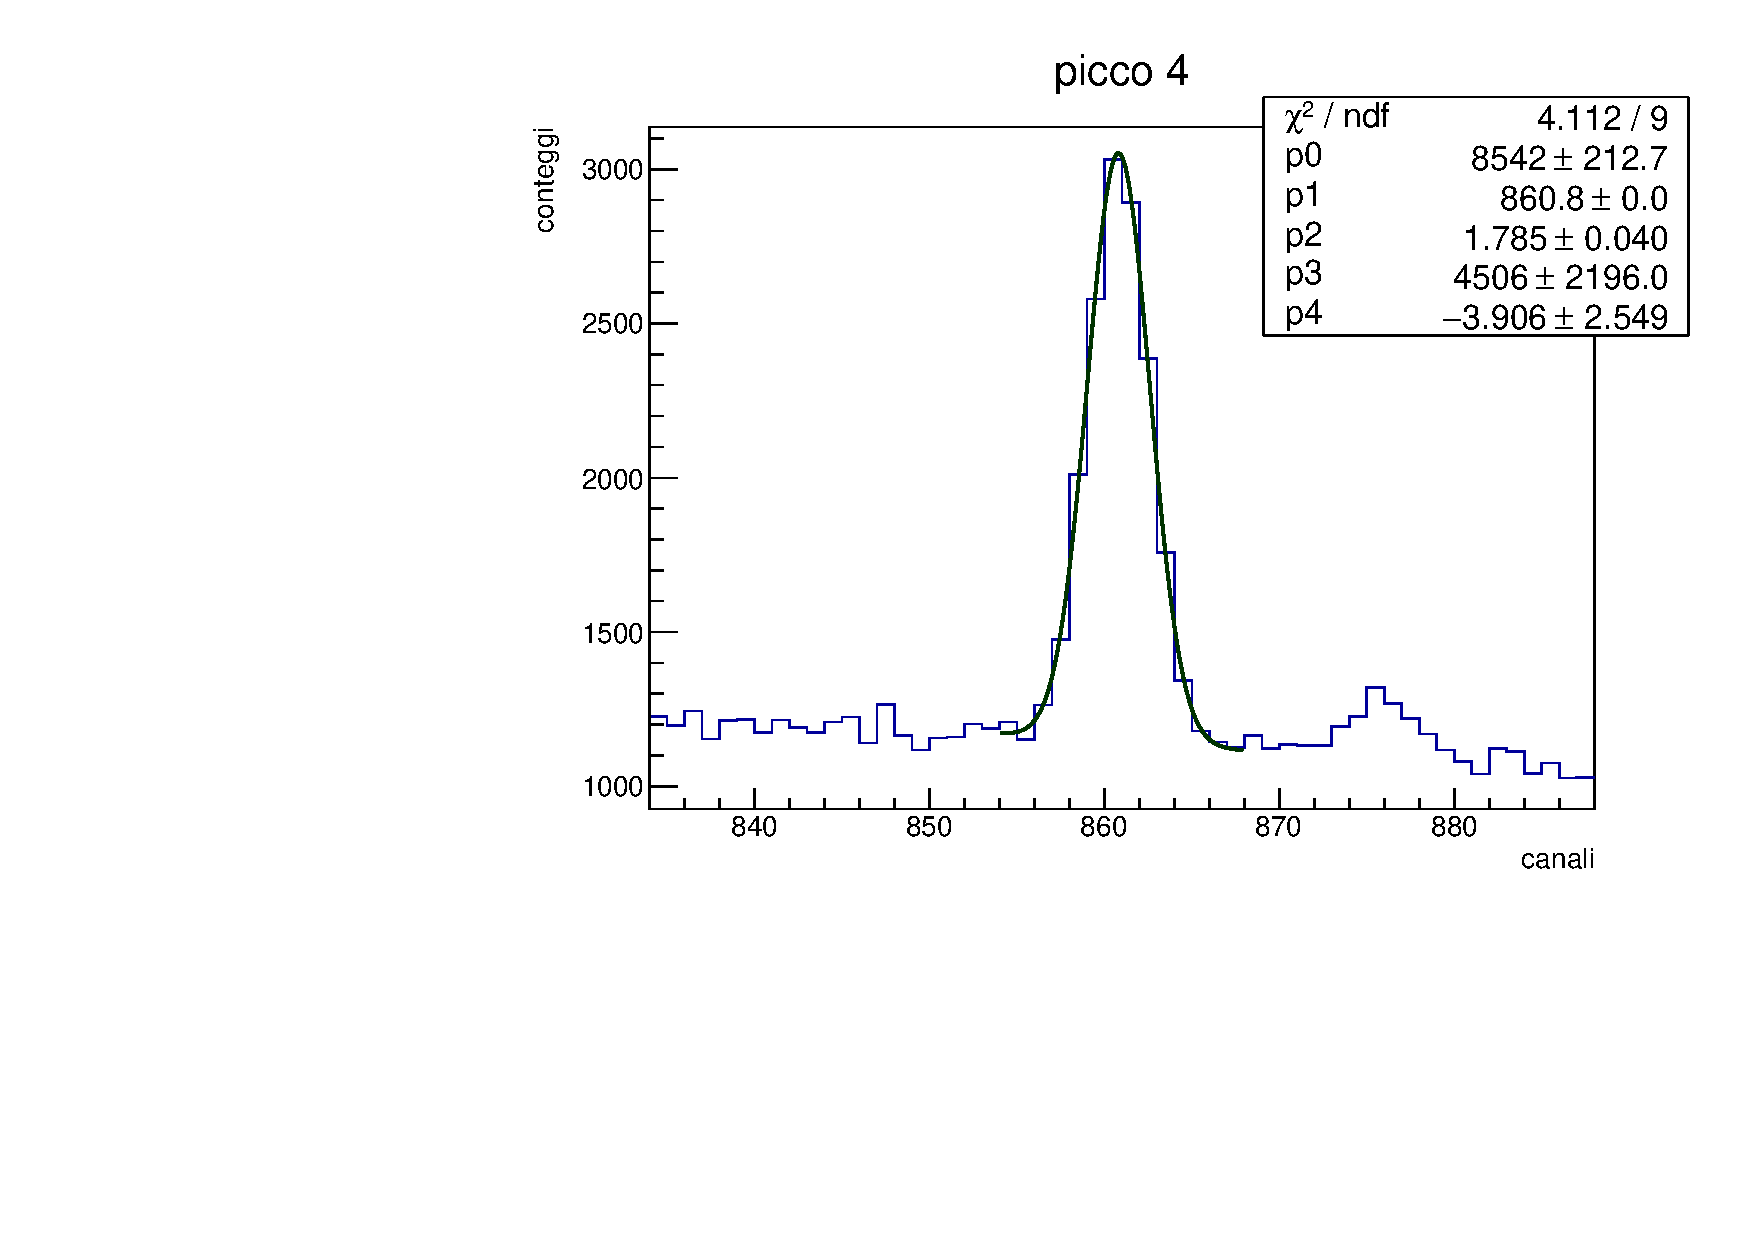
\includegraphics[width=2.2cm]{grafici/picco_incognita_germanio_4.pdf}
                    }
                \subfigure[picco 5]
                    {
                        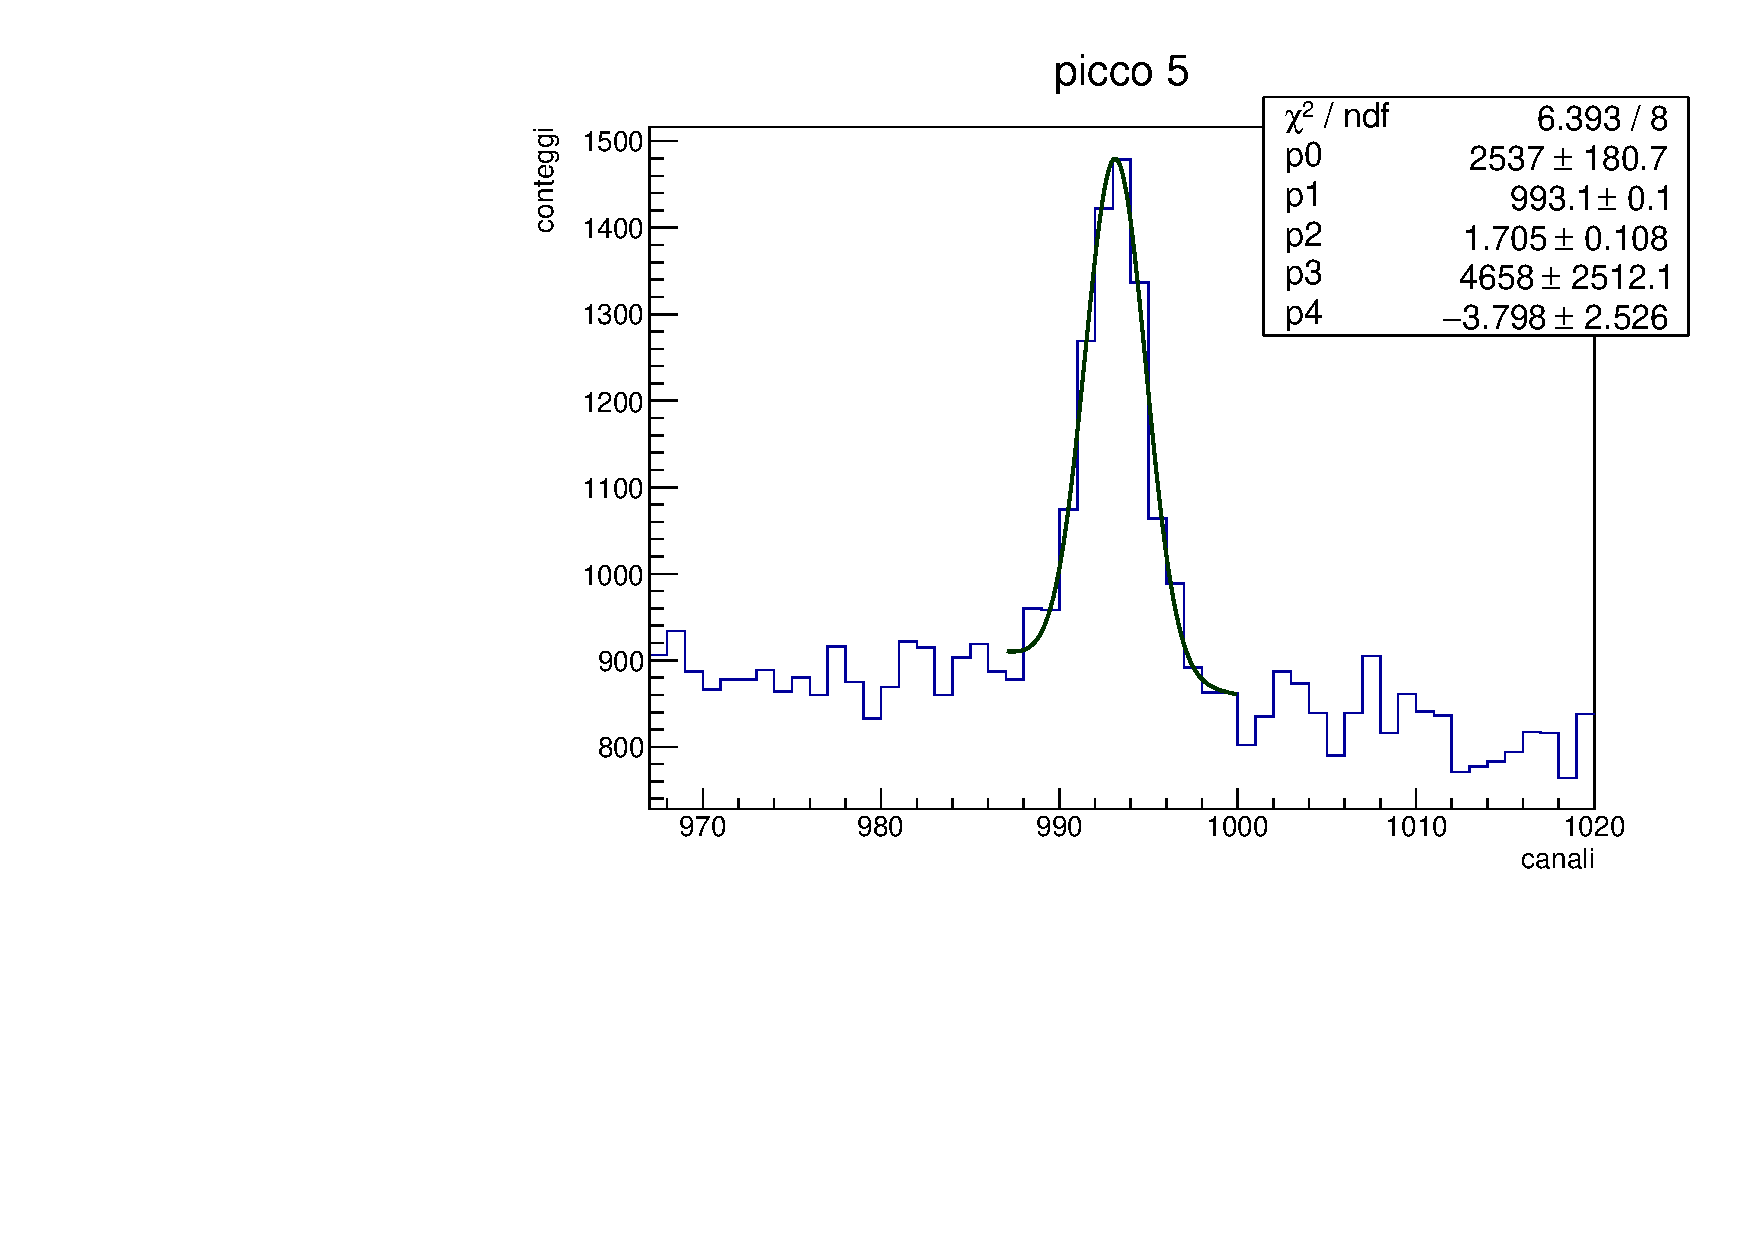
\includegraphics[width=2.2cm]{grafici/picco_incognita_germanio_5.pdf}
                    }

                \subfigure[picco 6]
                    {
                        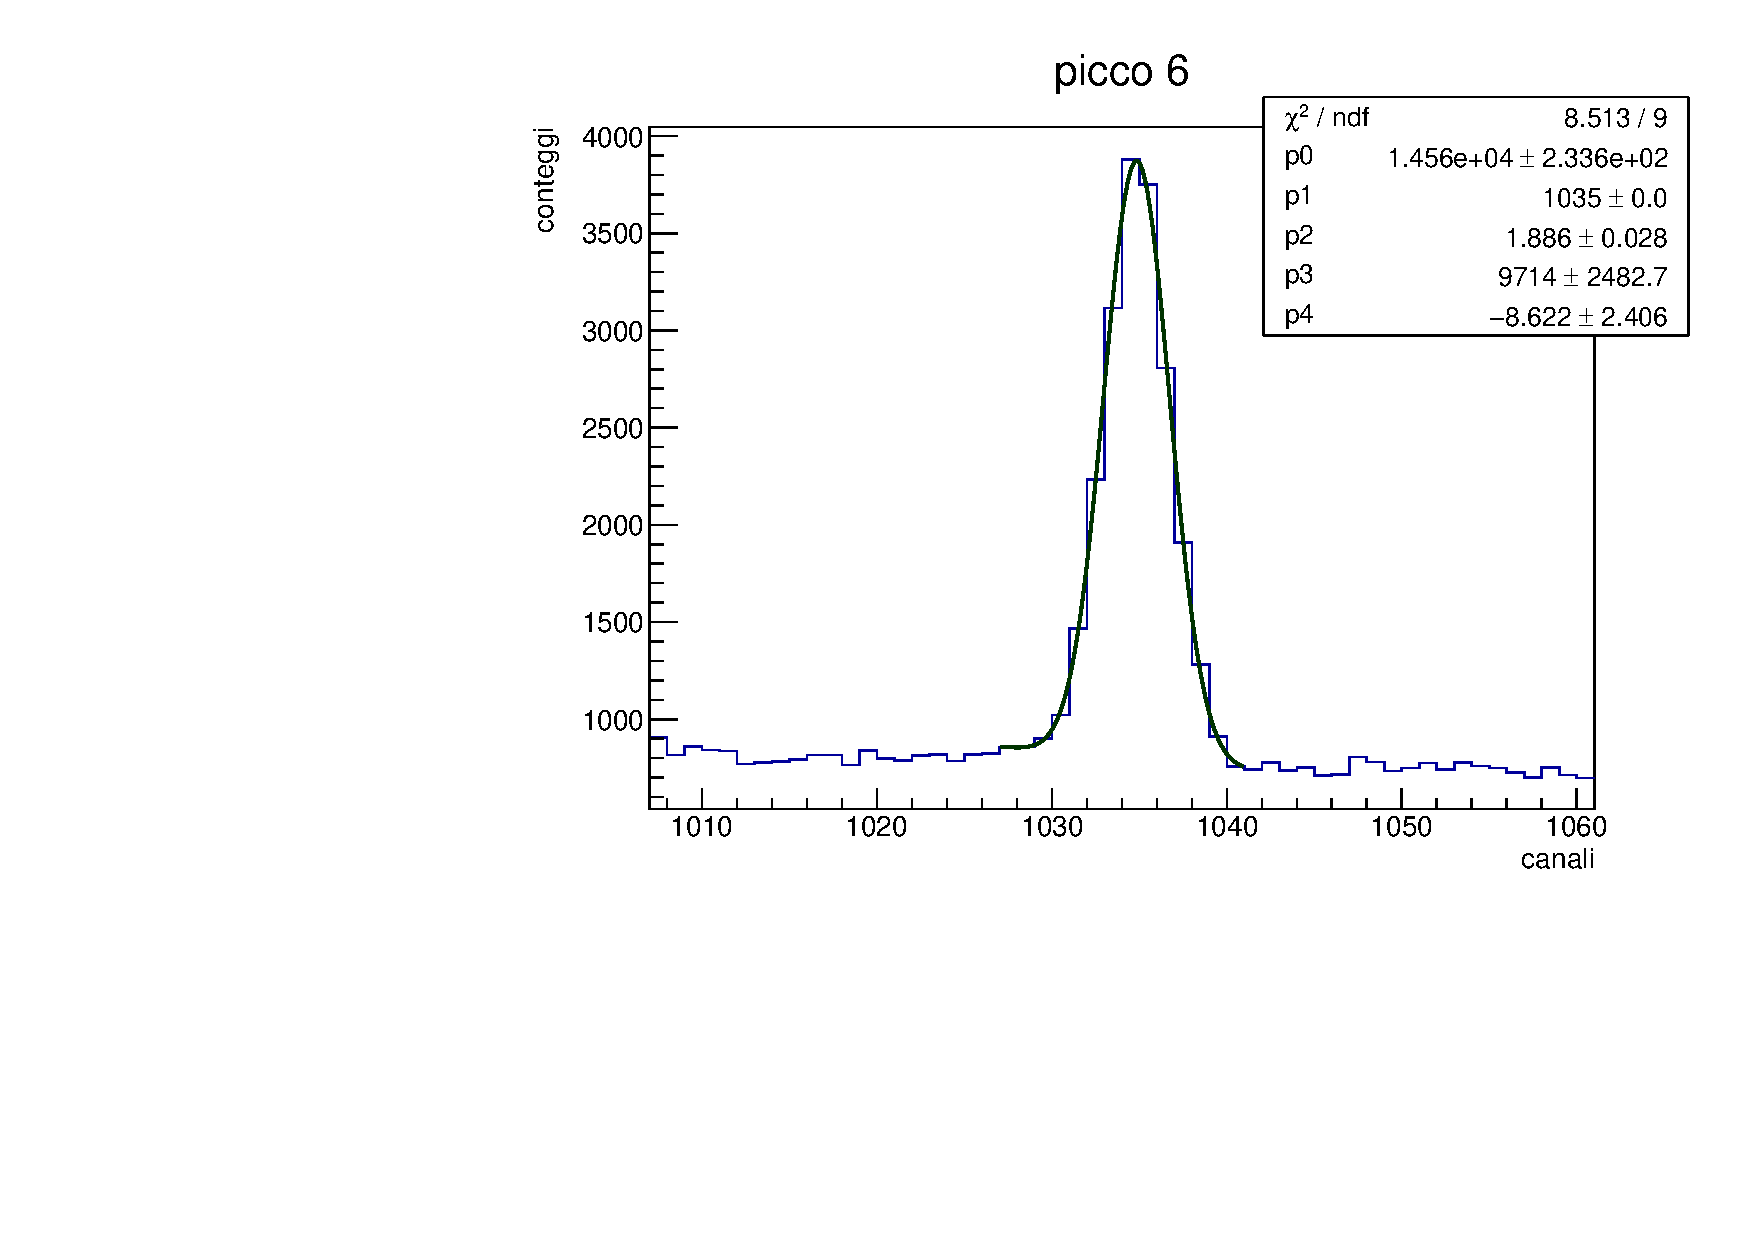
\includegraphics[width=2.2cm]{grafici/picco_incognita_germanio_6.pdf}
                    }
                \subfigure[picco 7]
                    {
                        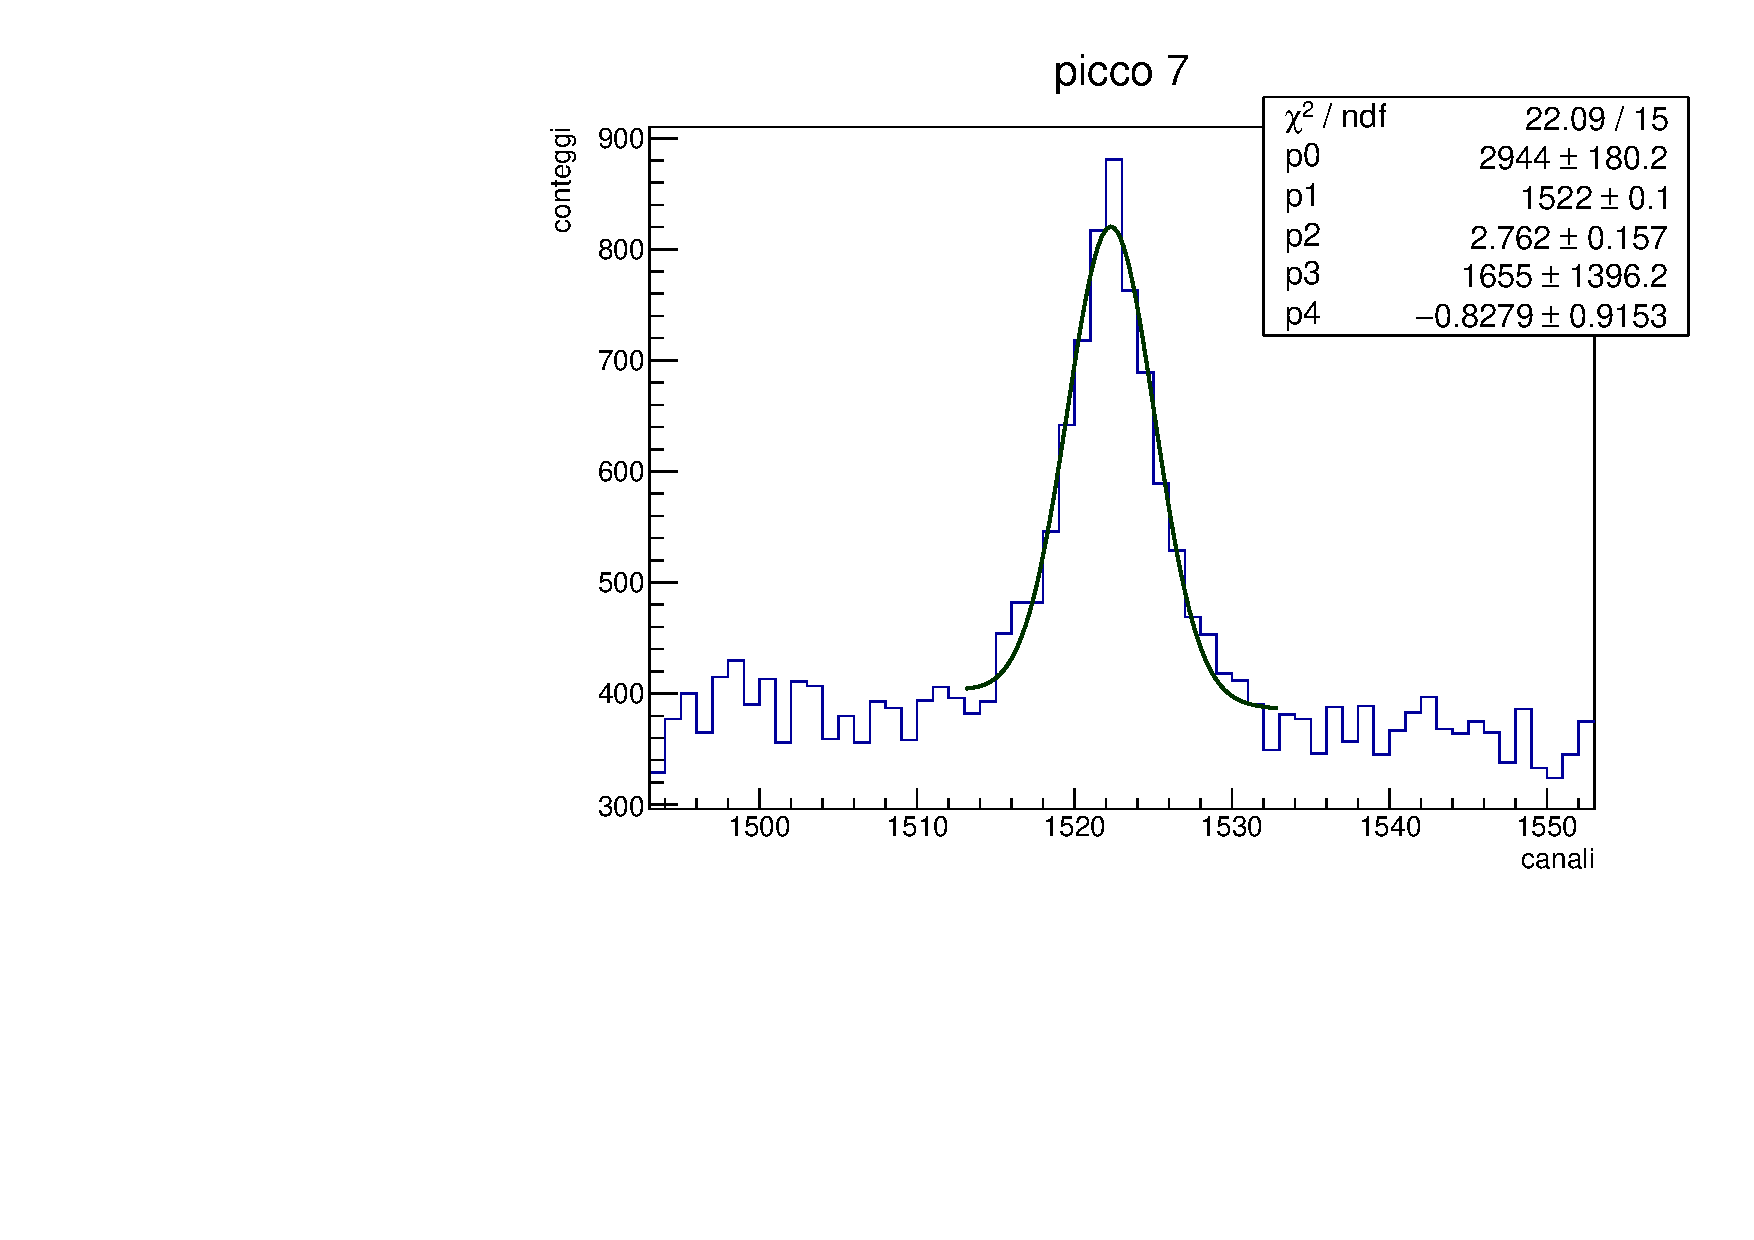
\includegraphics[width=2.2cm]{grafici/picco_incognita_germanio_7.pdf}
                    }
                \subfigure[picco 8]
                    {
                        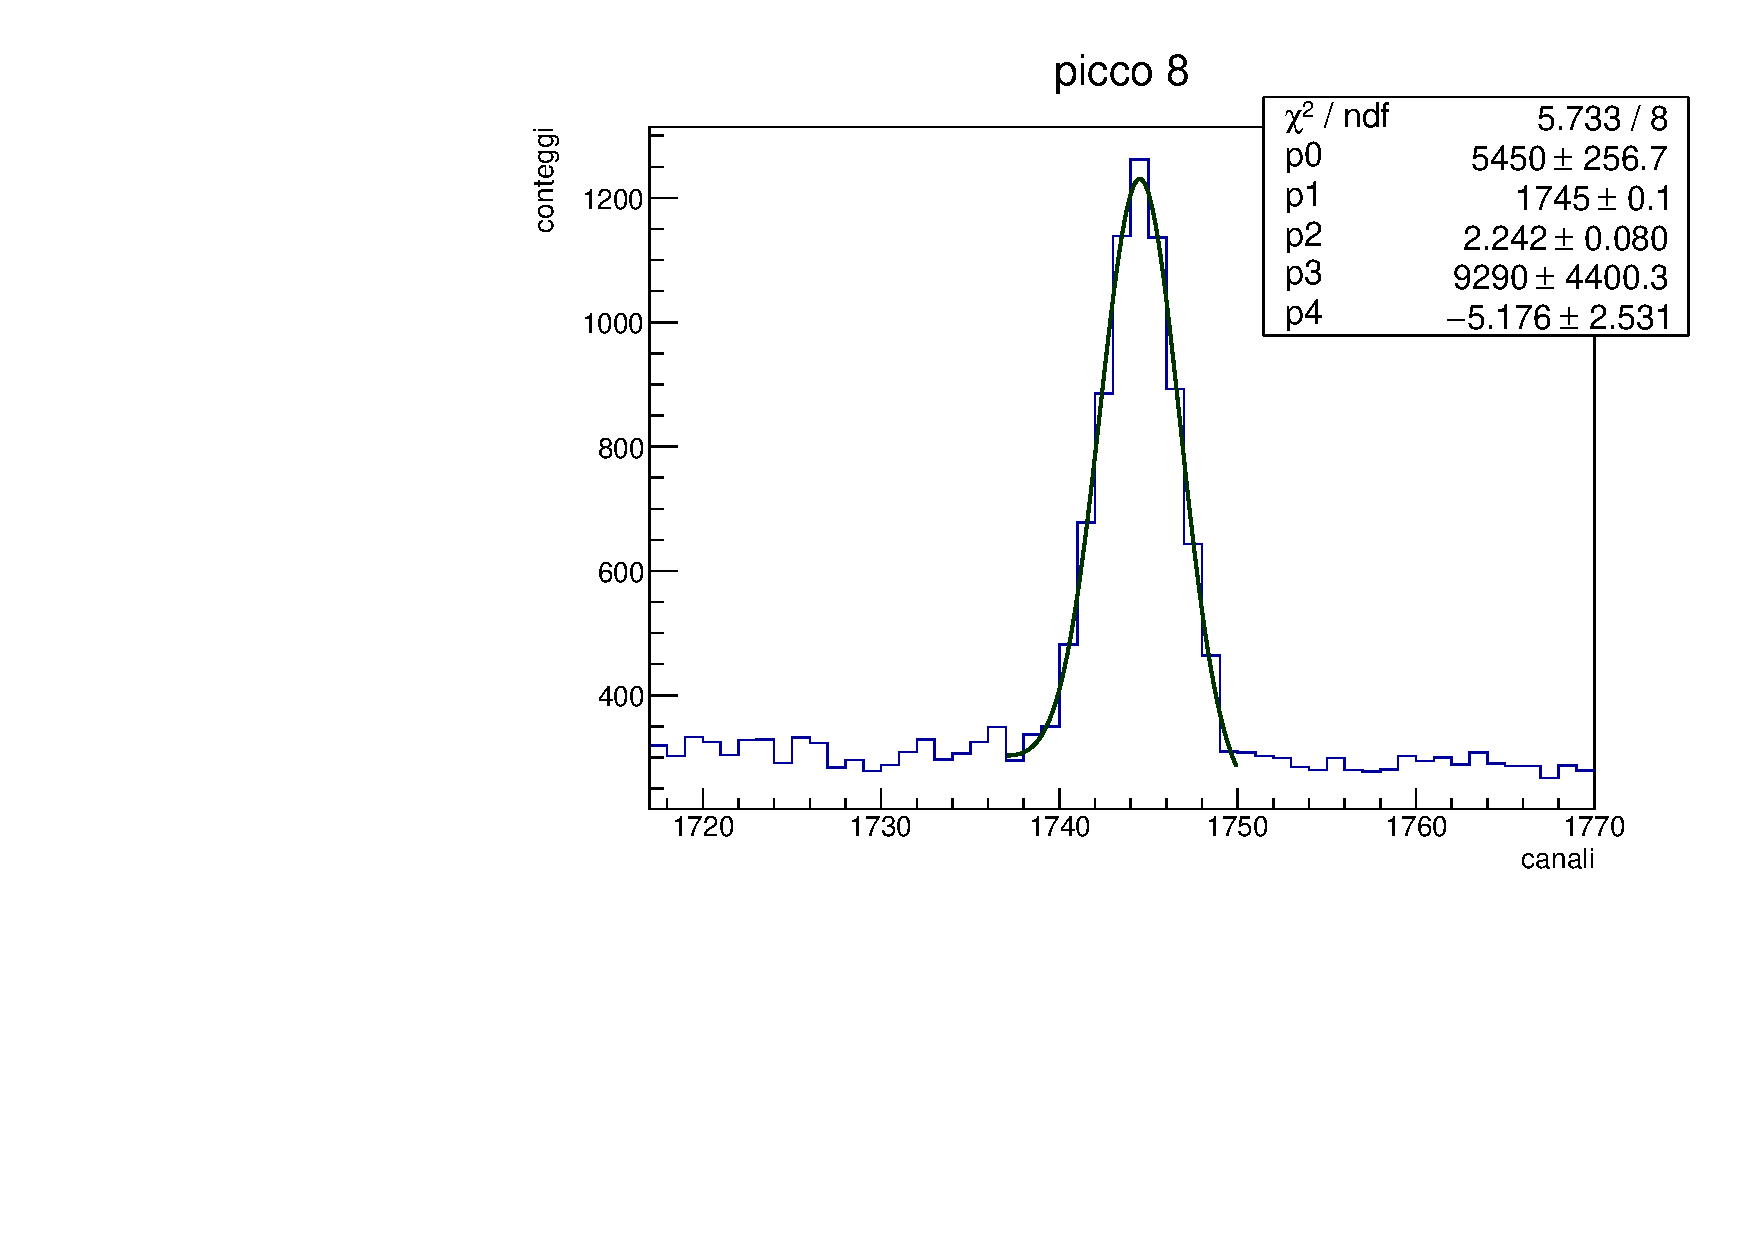
\includegraphics[width=2.2cm]{grafici/picco_incognita_germanio_8.pdf}
                    }
                \subfigure[picco 9]
                    {
                        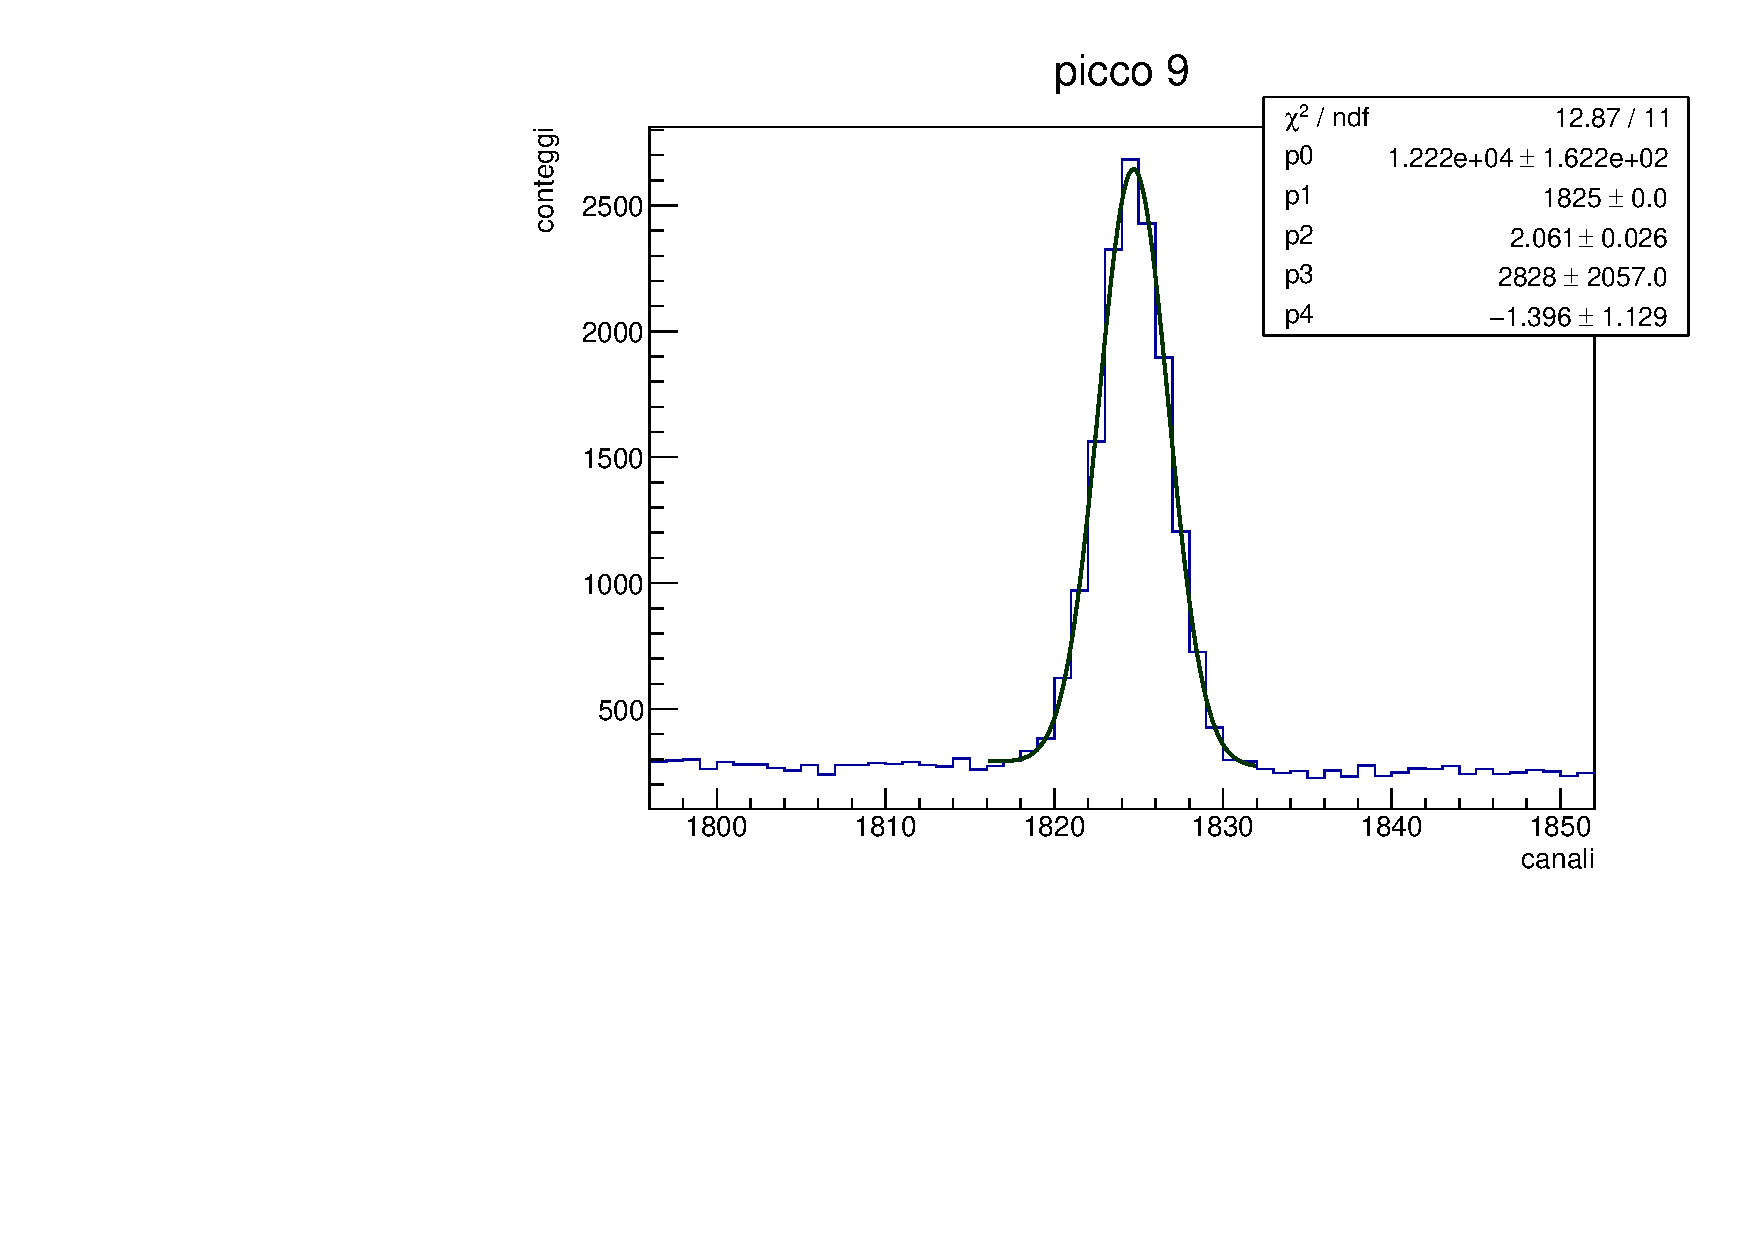
\includegraphics[width=2.2cm]{grafici/picco_incognita_germanio_9.pdf}
                    }
                \subfigure[picco 10]
                    {
                        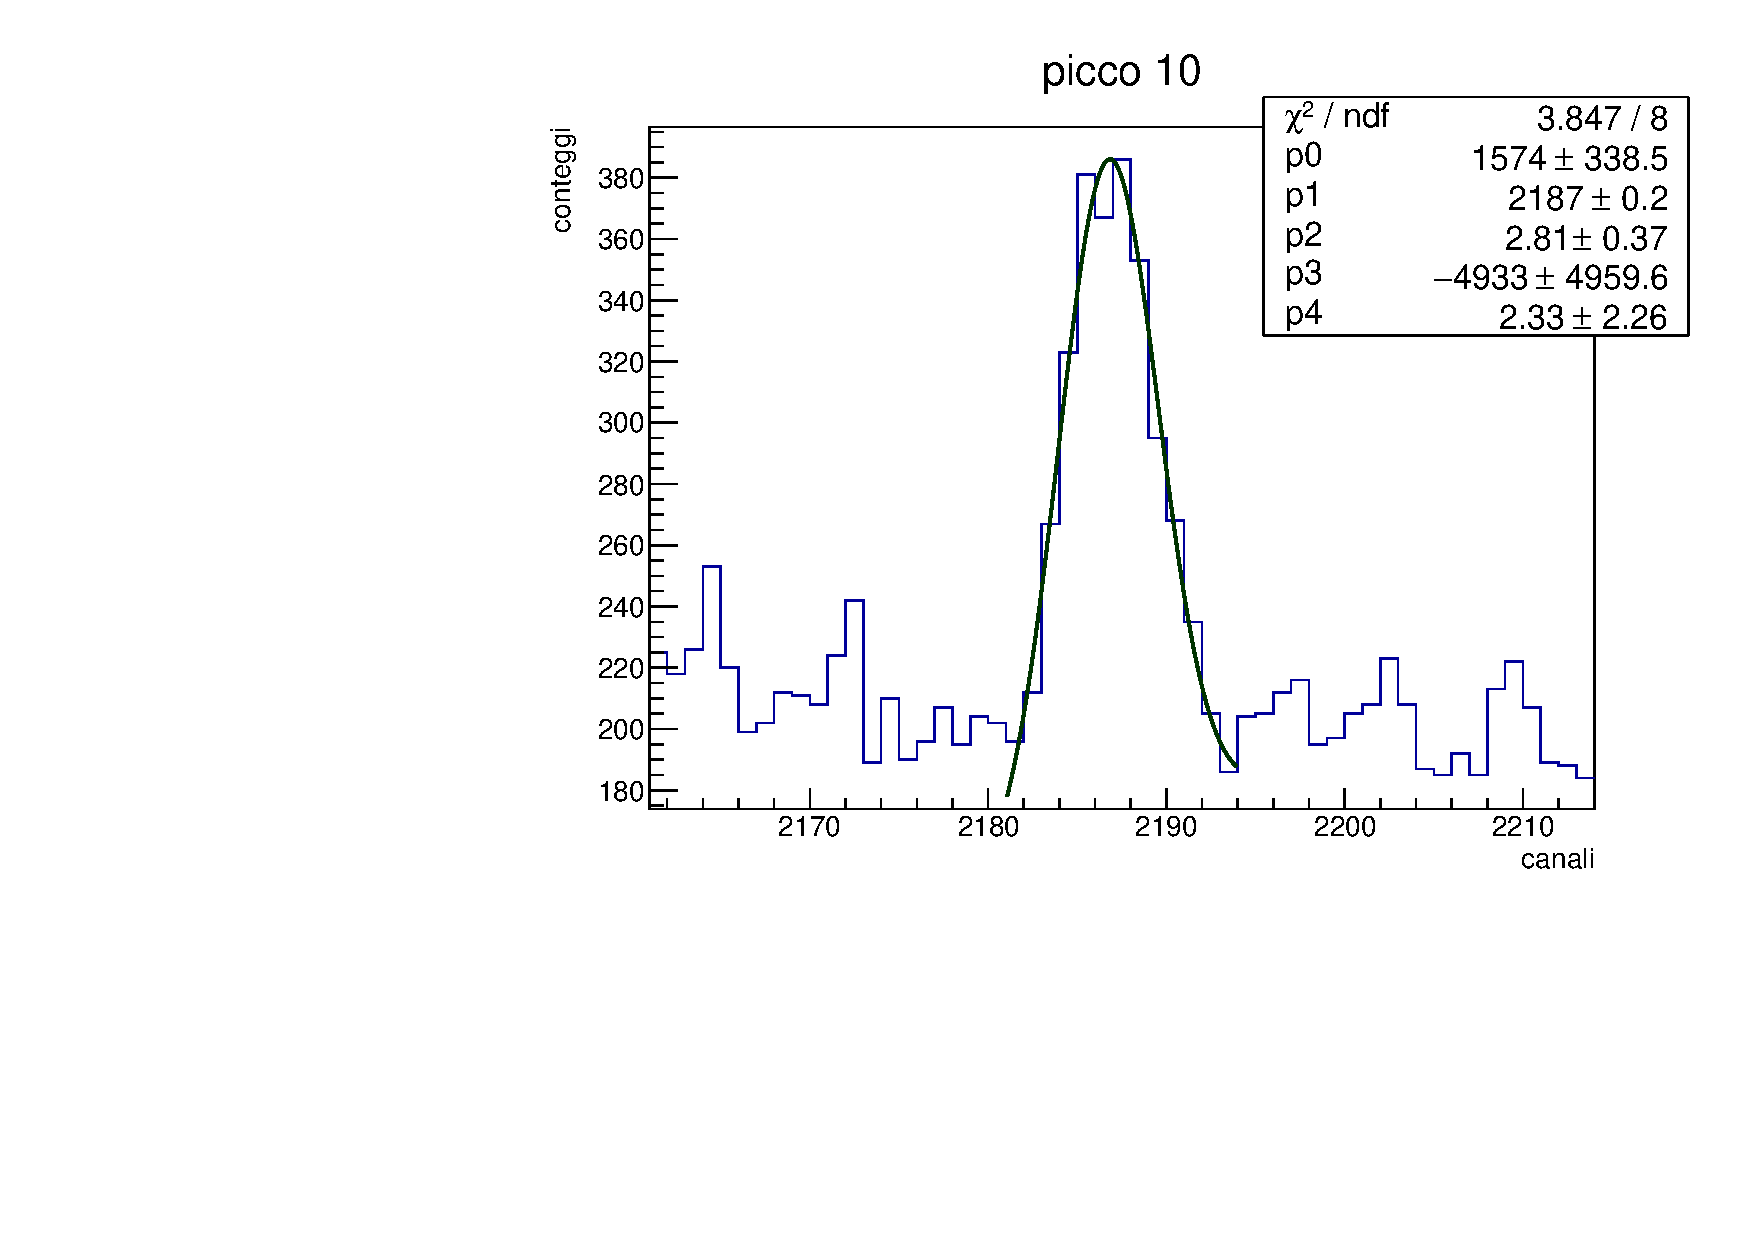
\includegraphics[width=2.2cm]{grafici/picco_incognita_germanio_10.pdf}
                    }

                \subfigure[picco 11]
                    {
                        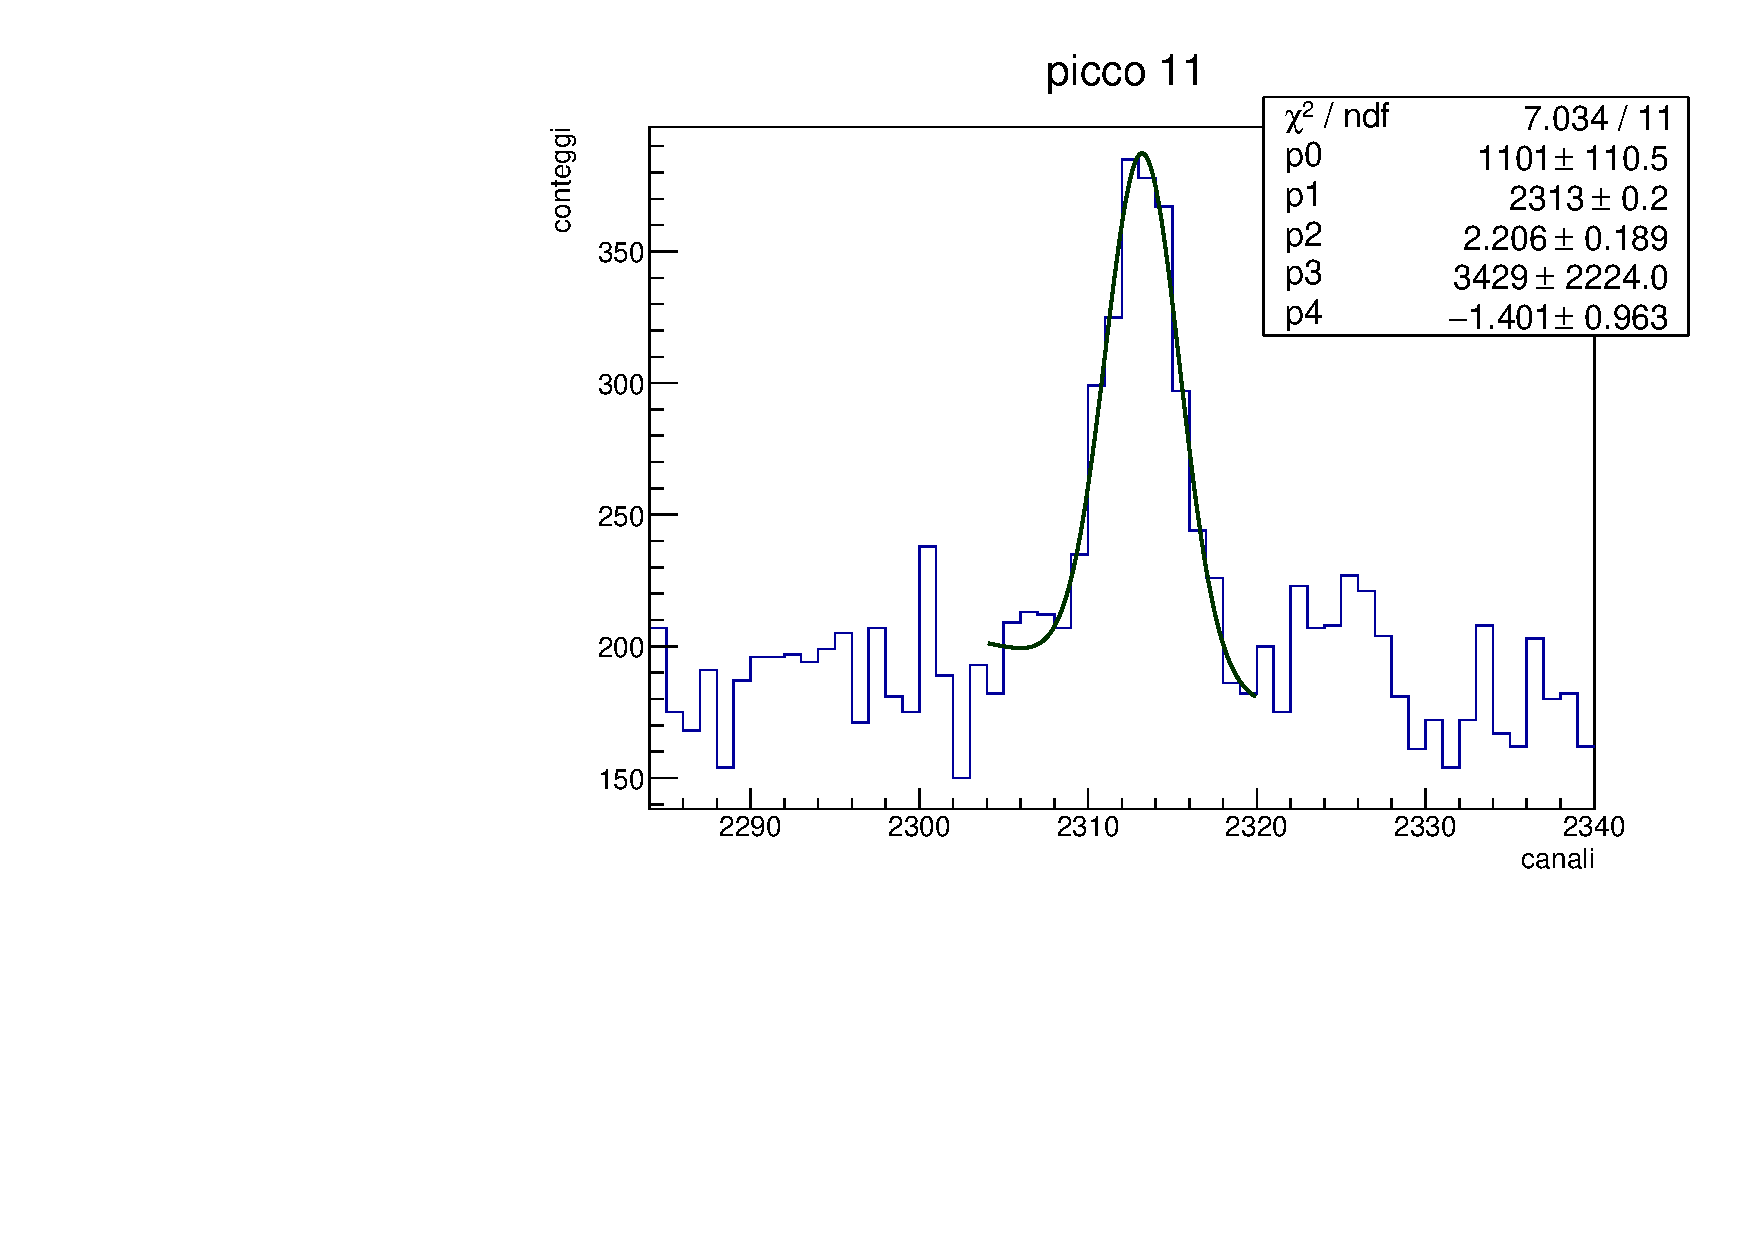
\includegraphics[width=2.2cm]{grafici/picco_incognita_germanio_11.pdf}
                    }
                \subfigure[picco 12]
                    {
                        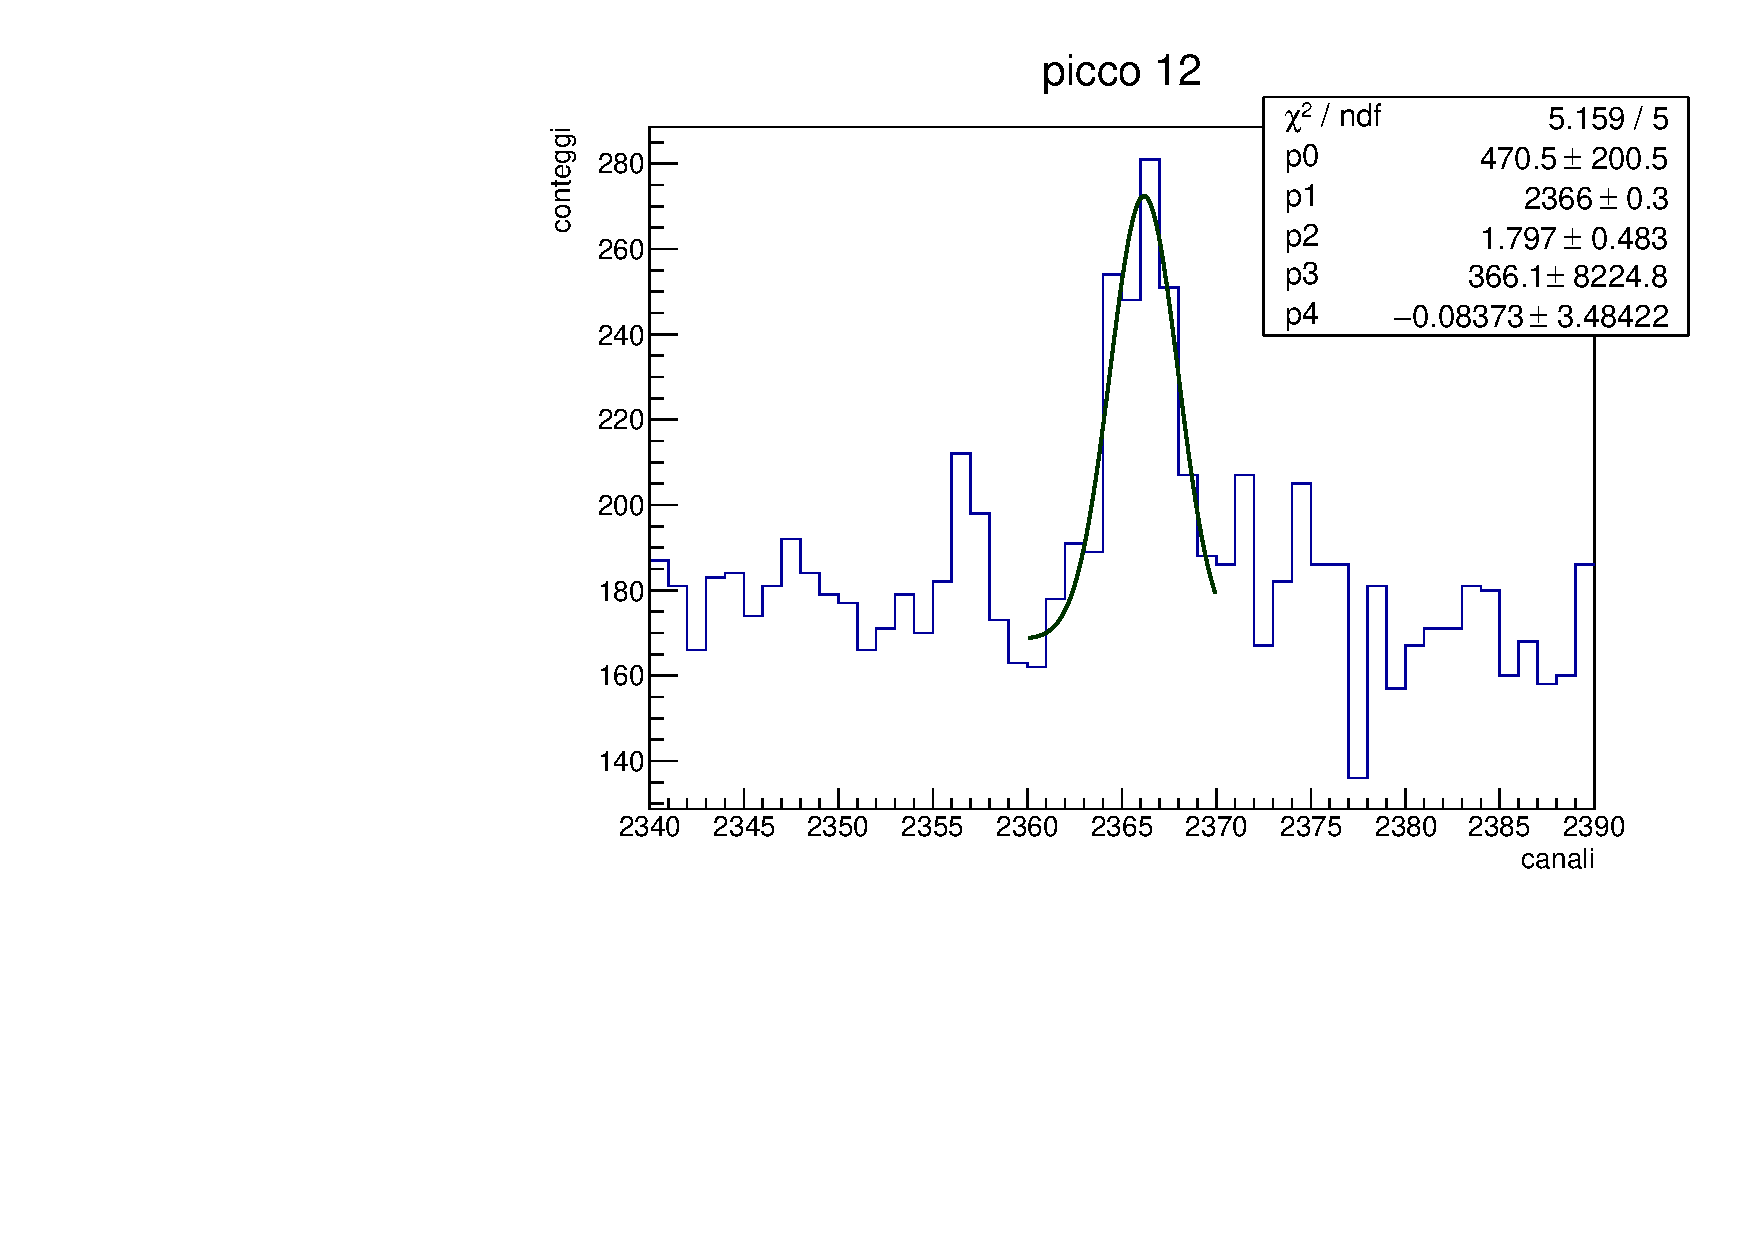
\includegraphics[width=2.2cm]{grafici/picco_incognita_germanio_12.pdf}
                    }
                \subfigure[picco 13]
                    {
                        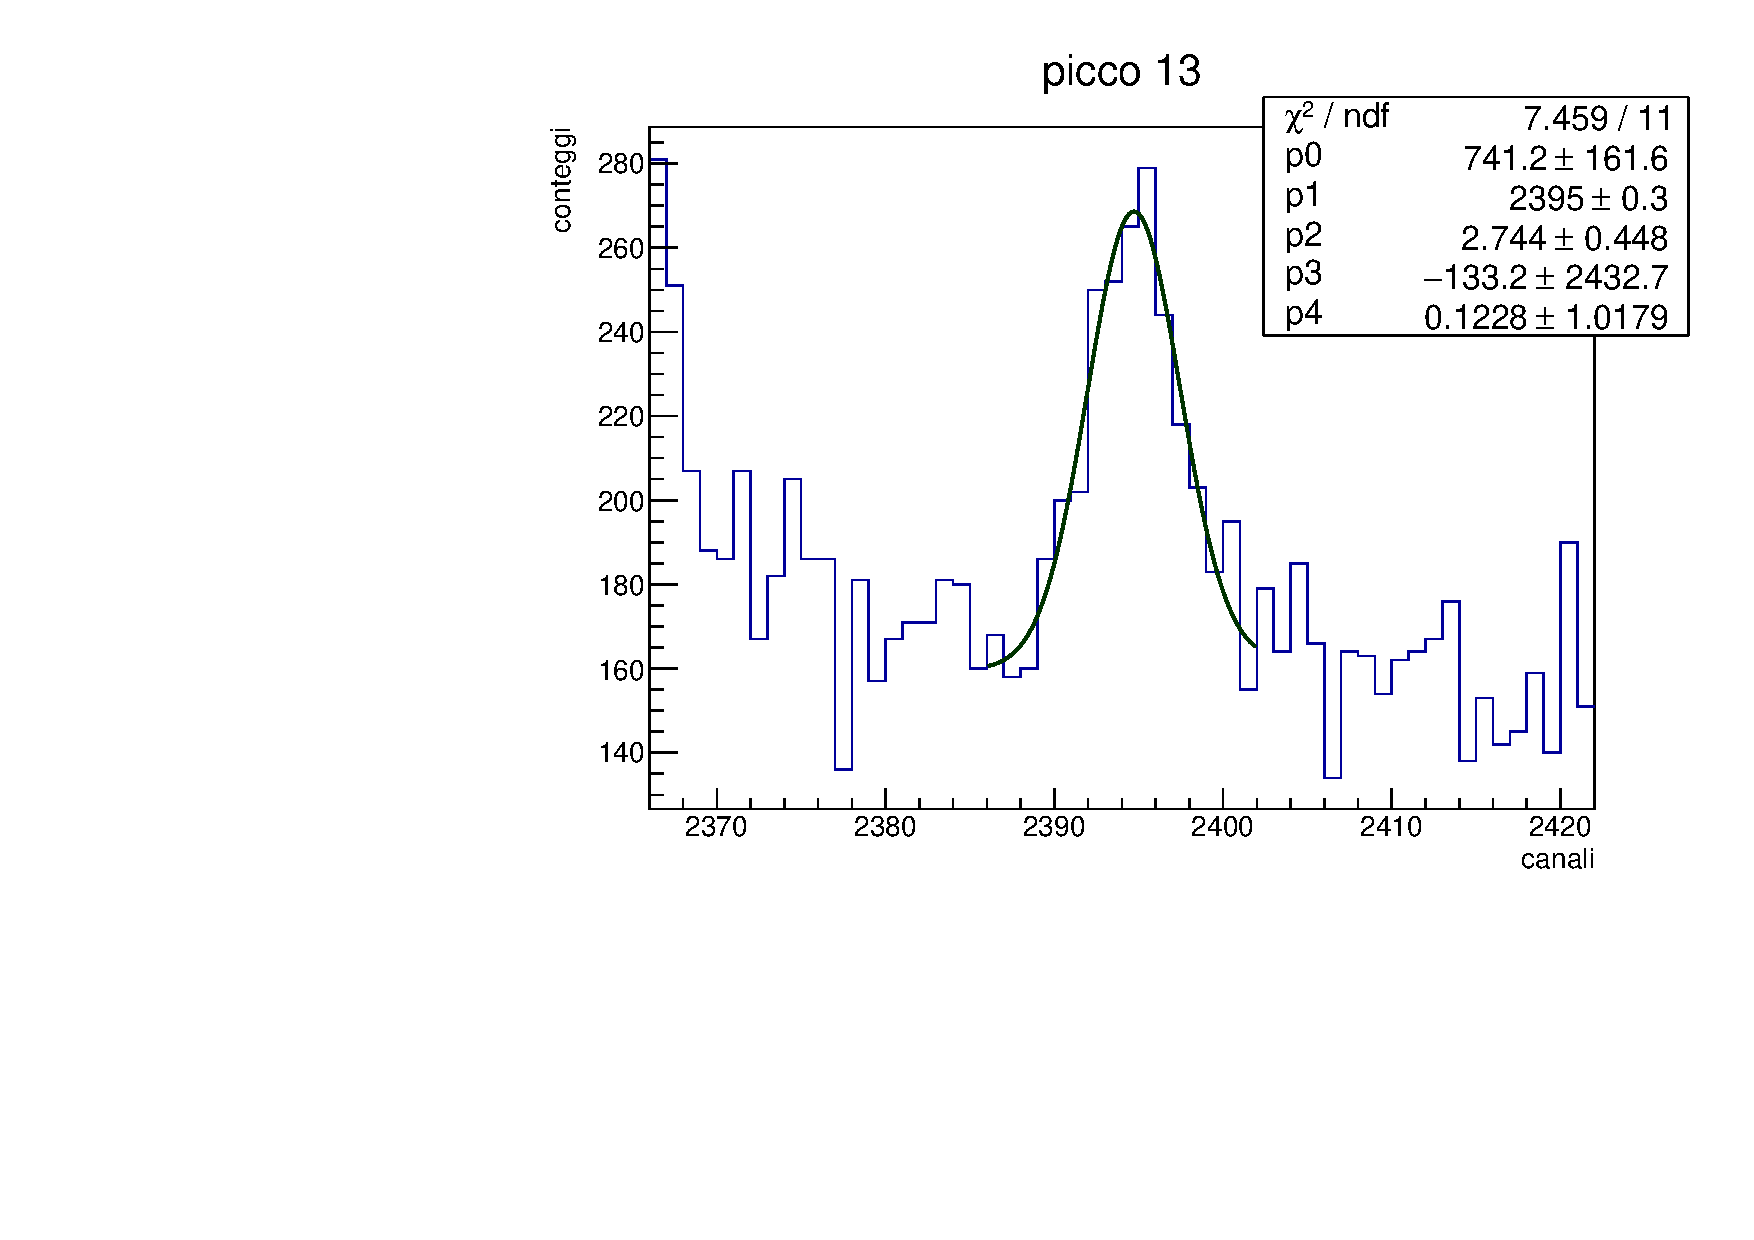
\includegraphics[width=2.2cm]{grafici/picco_incognita_germanio_13.pdf}
                    }
                \subfigure[picco 14]
                    {
                        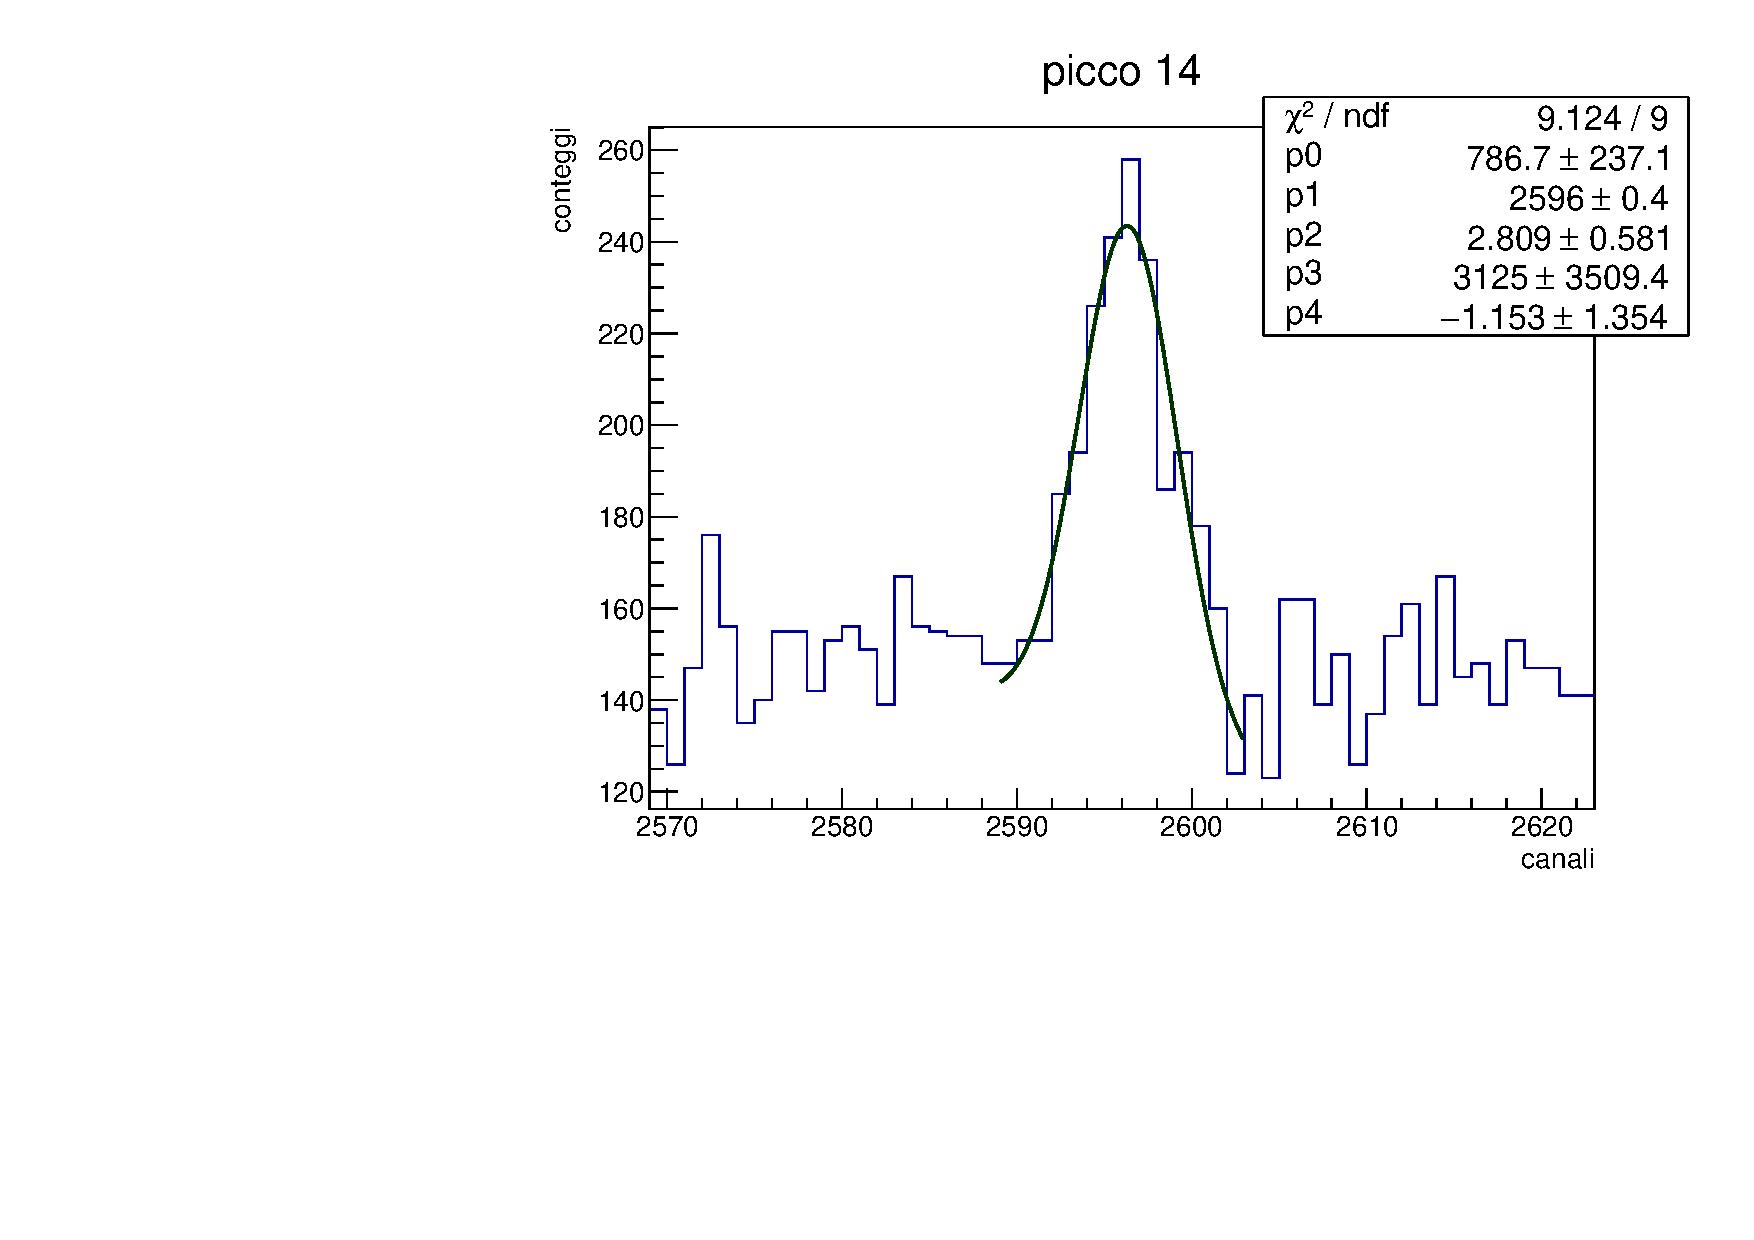
\includegraphics[width=2.2cm]{grafici/picco_incognita_germanio_14.pdf}
                    }
                \subfigure[picco 15]
                    {
                        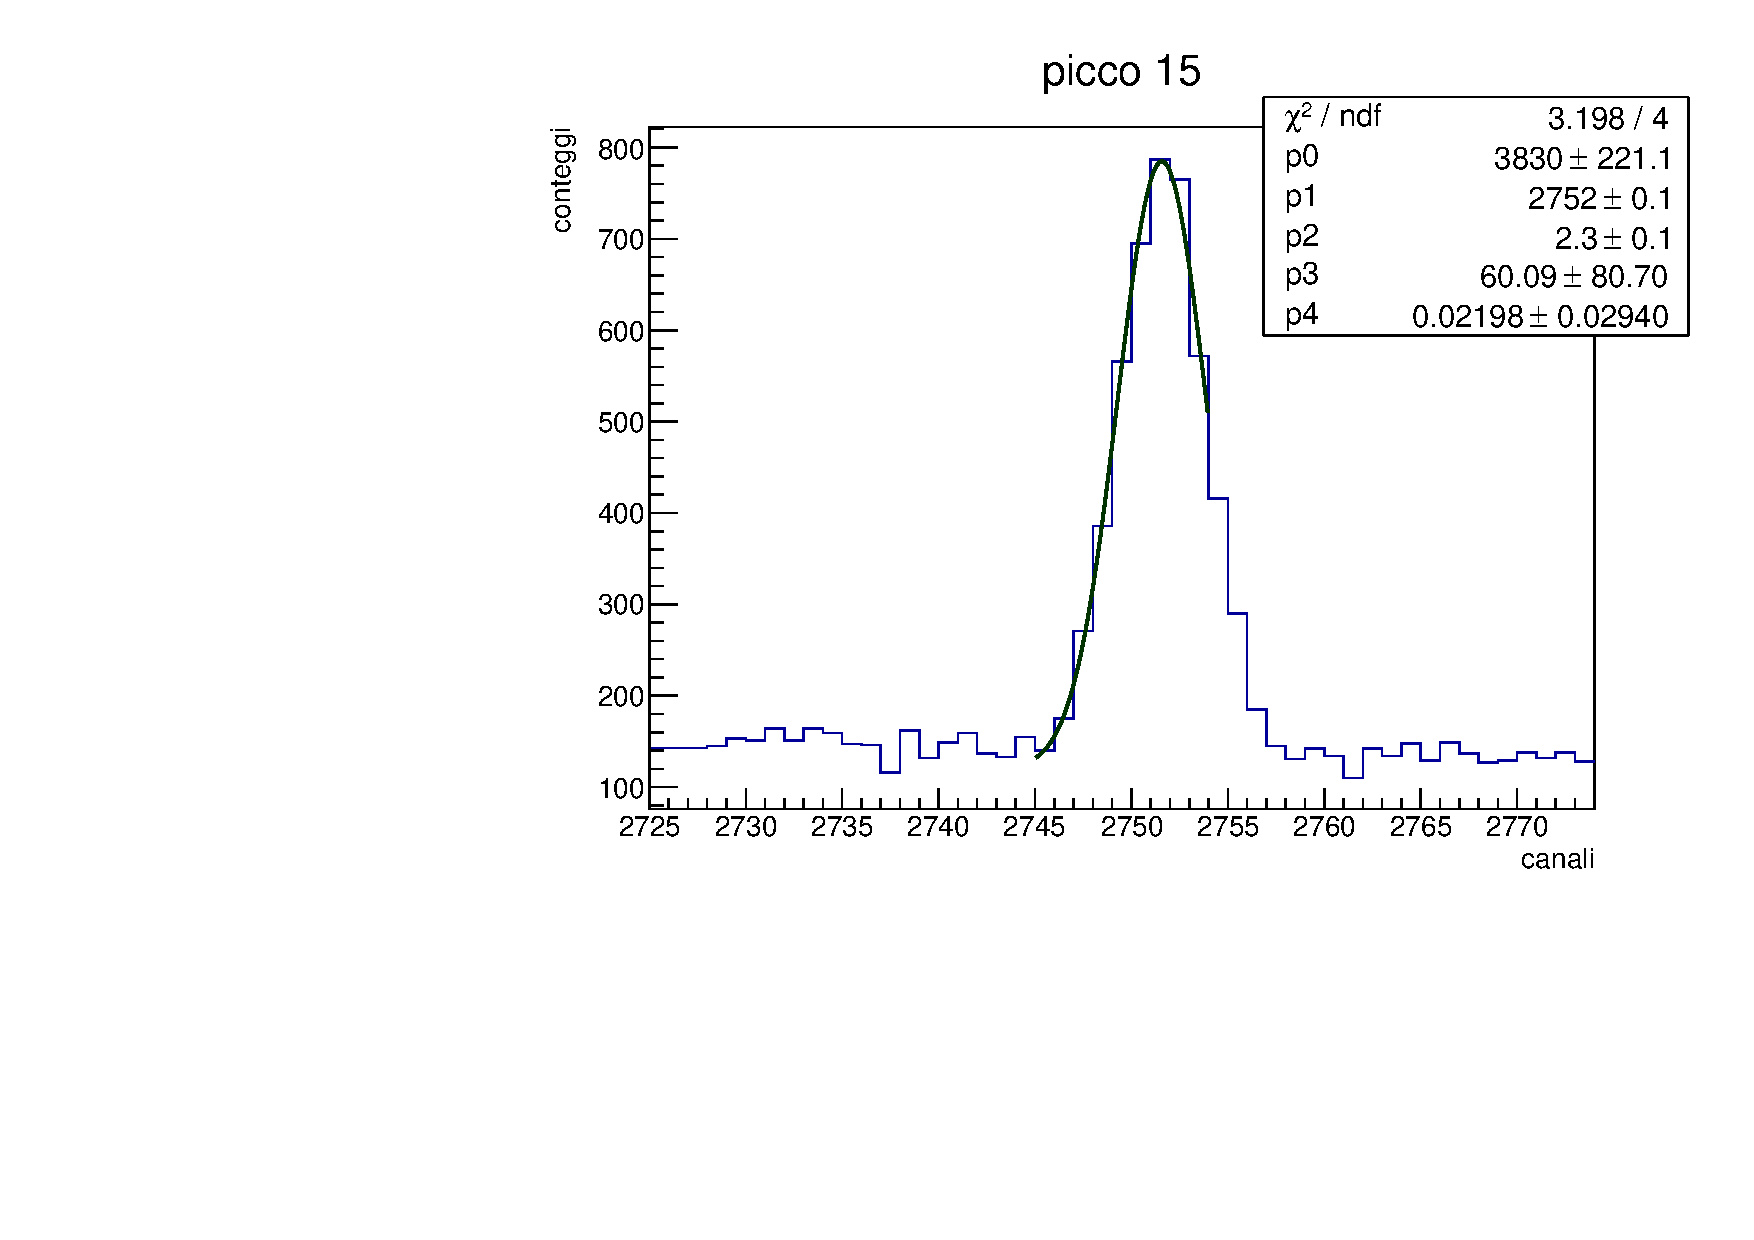
\includegraphics[width=2.2cm]{grafici/picco_incognita_germanio_15.pdf}
                    }

                \subfigure[picco 16]
                    {
                        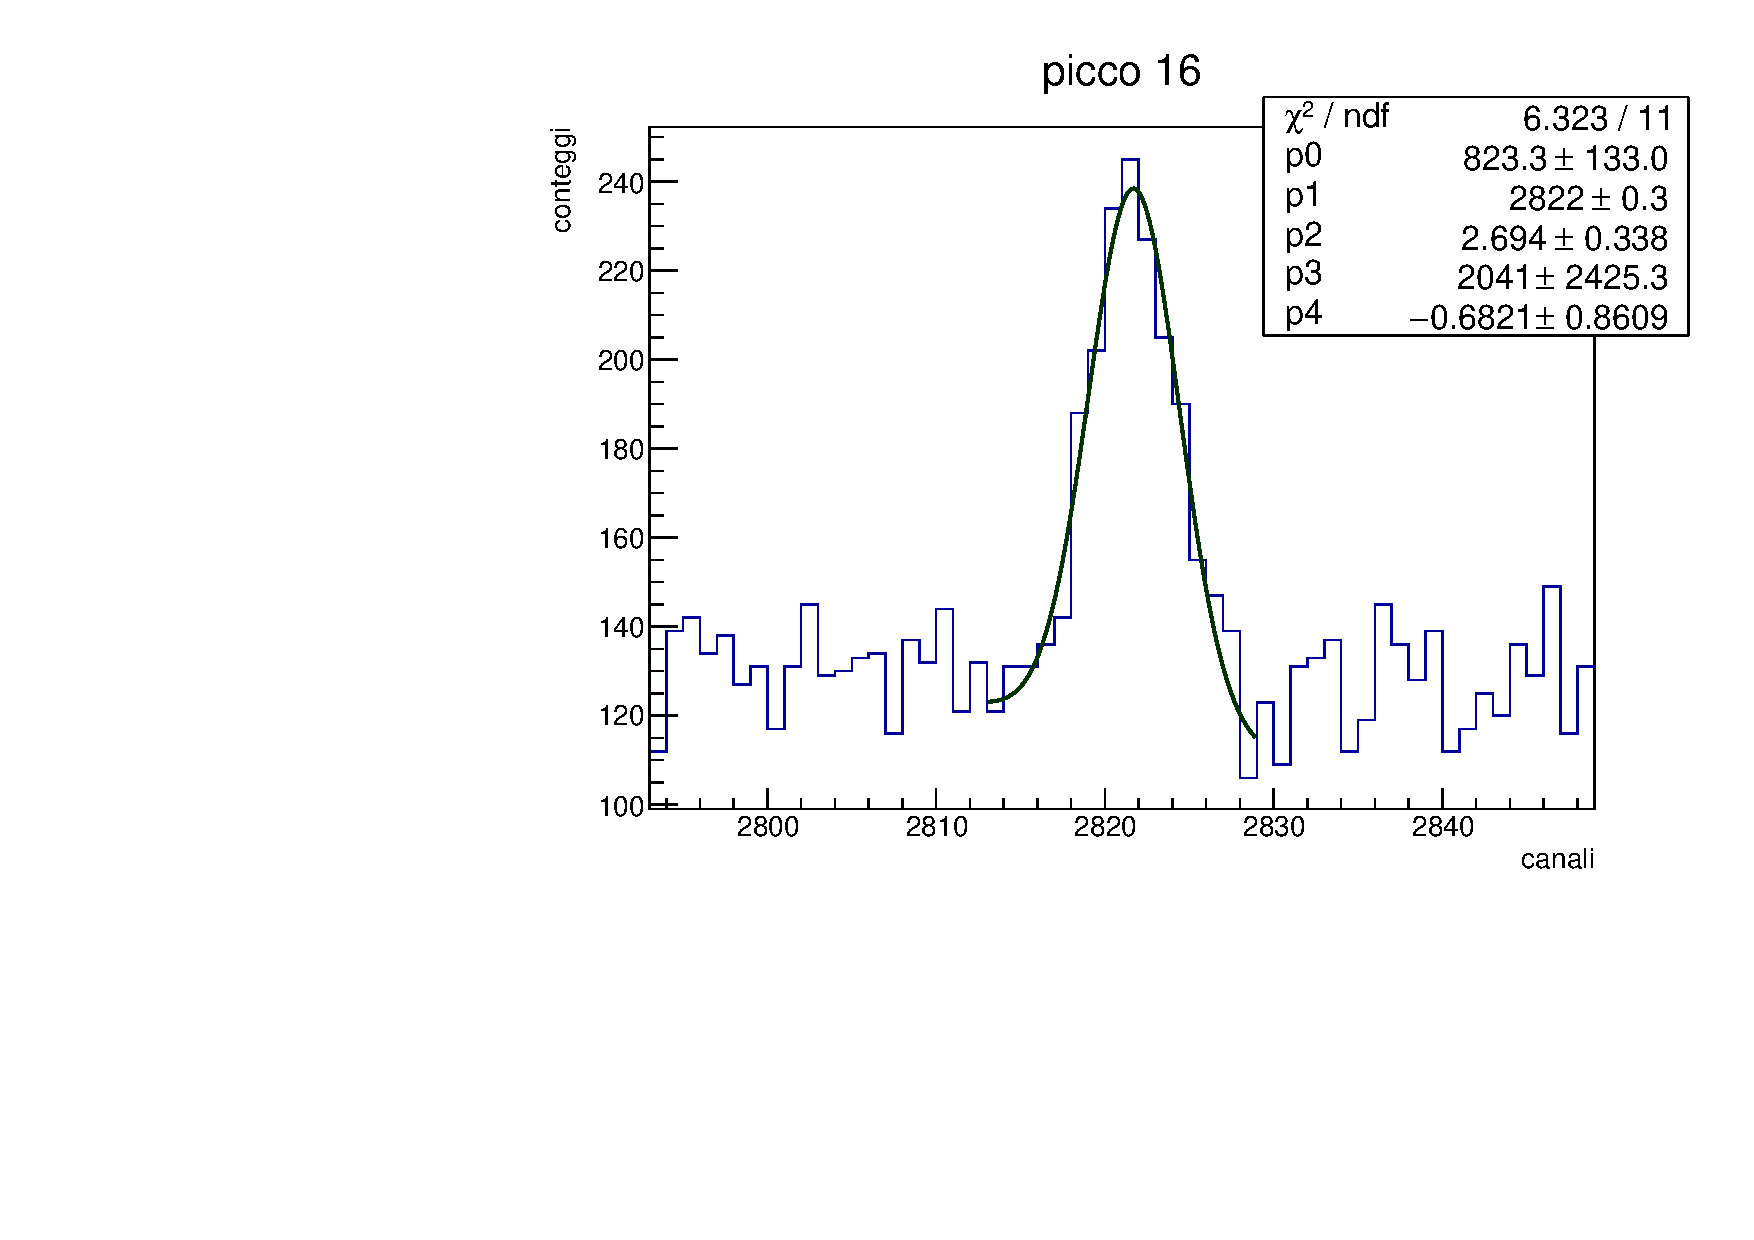
\includegraphics[width=2.2cm]{grafici/picco_incognita_germanio_16.pdf}
                    }
                \subfigure[picco 17]
                    {
                        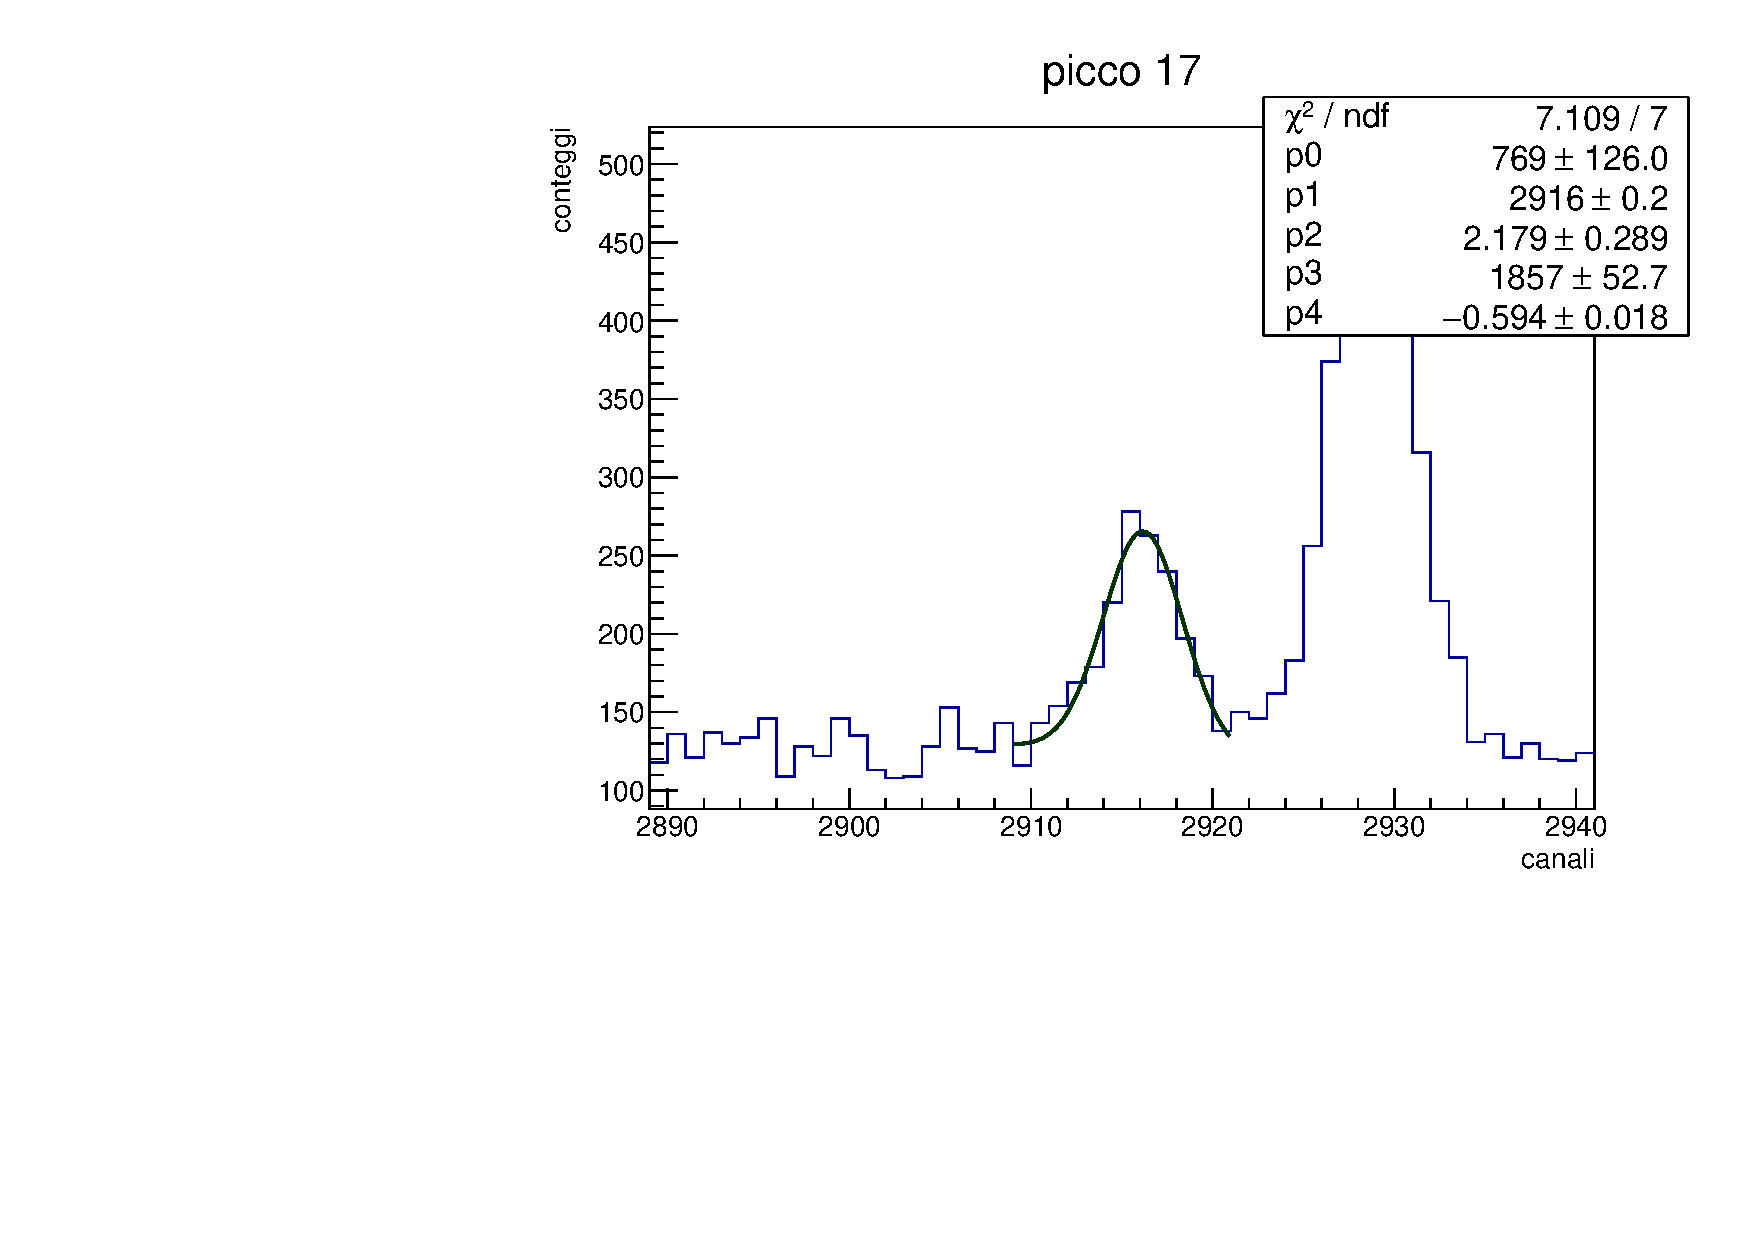
\includegraphics[width=2.2cm]{grafici/picco_incognita_germanio_17.pdf}
                    }
                \subfigure[picco 18]
                    {
                        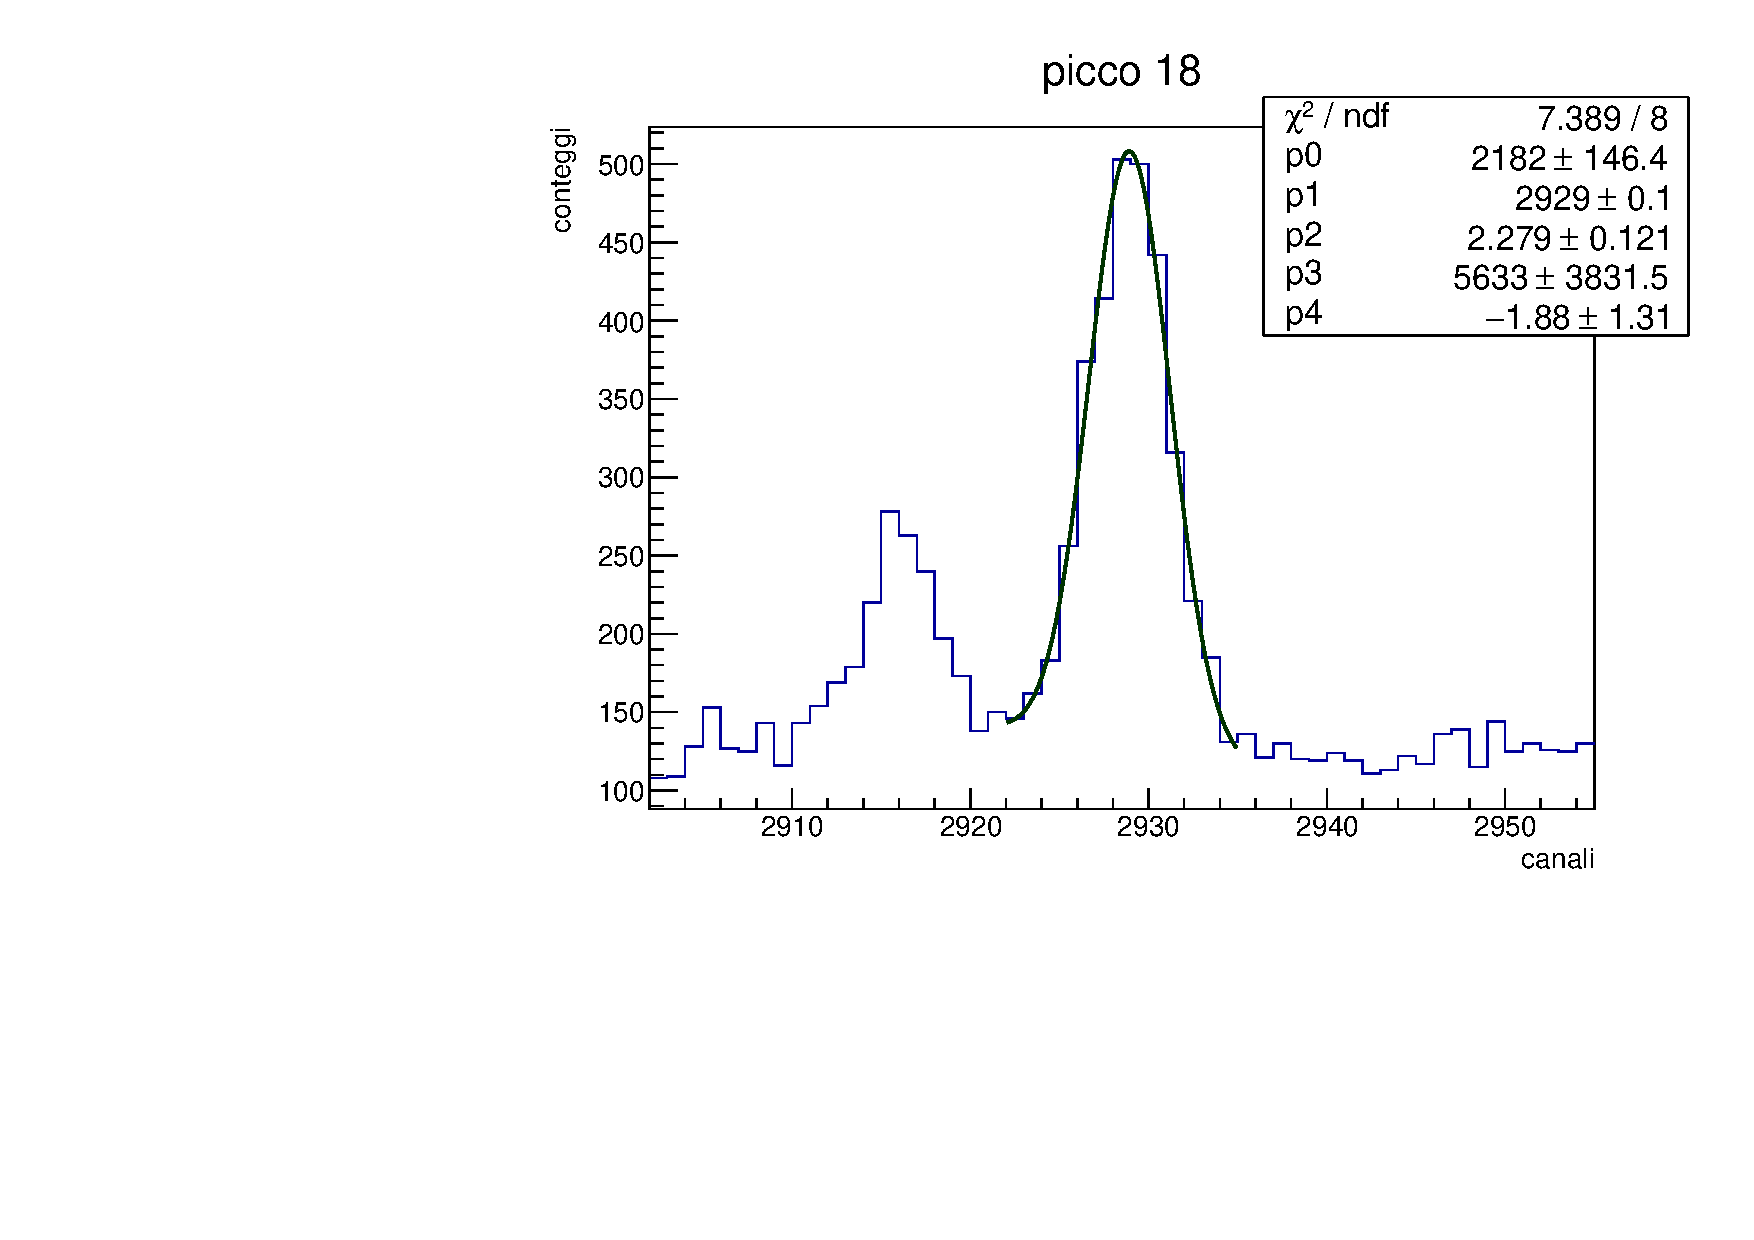
\includegraphics[width=2.2cm]{grafici/picco_incognita_germanio_18.pdf}
                    }
                \subfigure[picco 19]
                    {
                        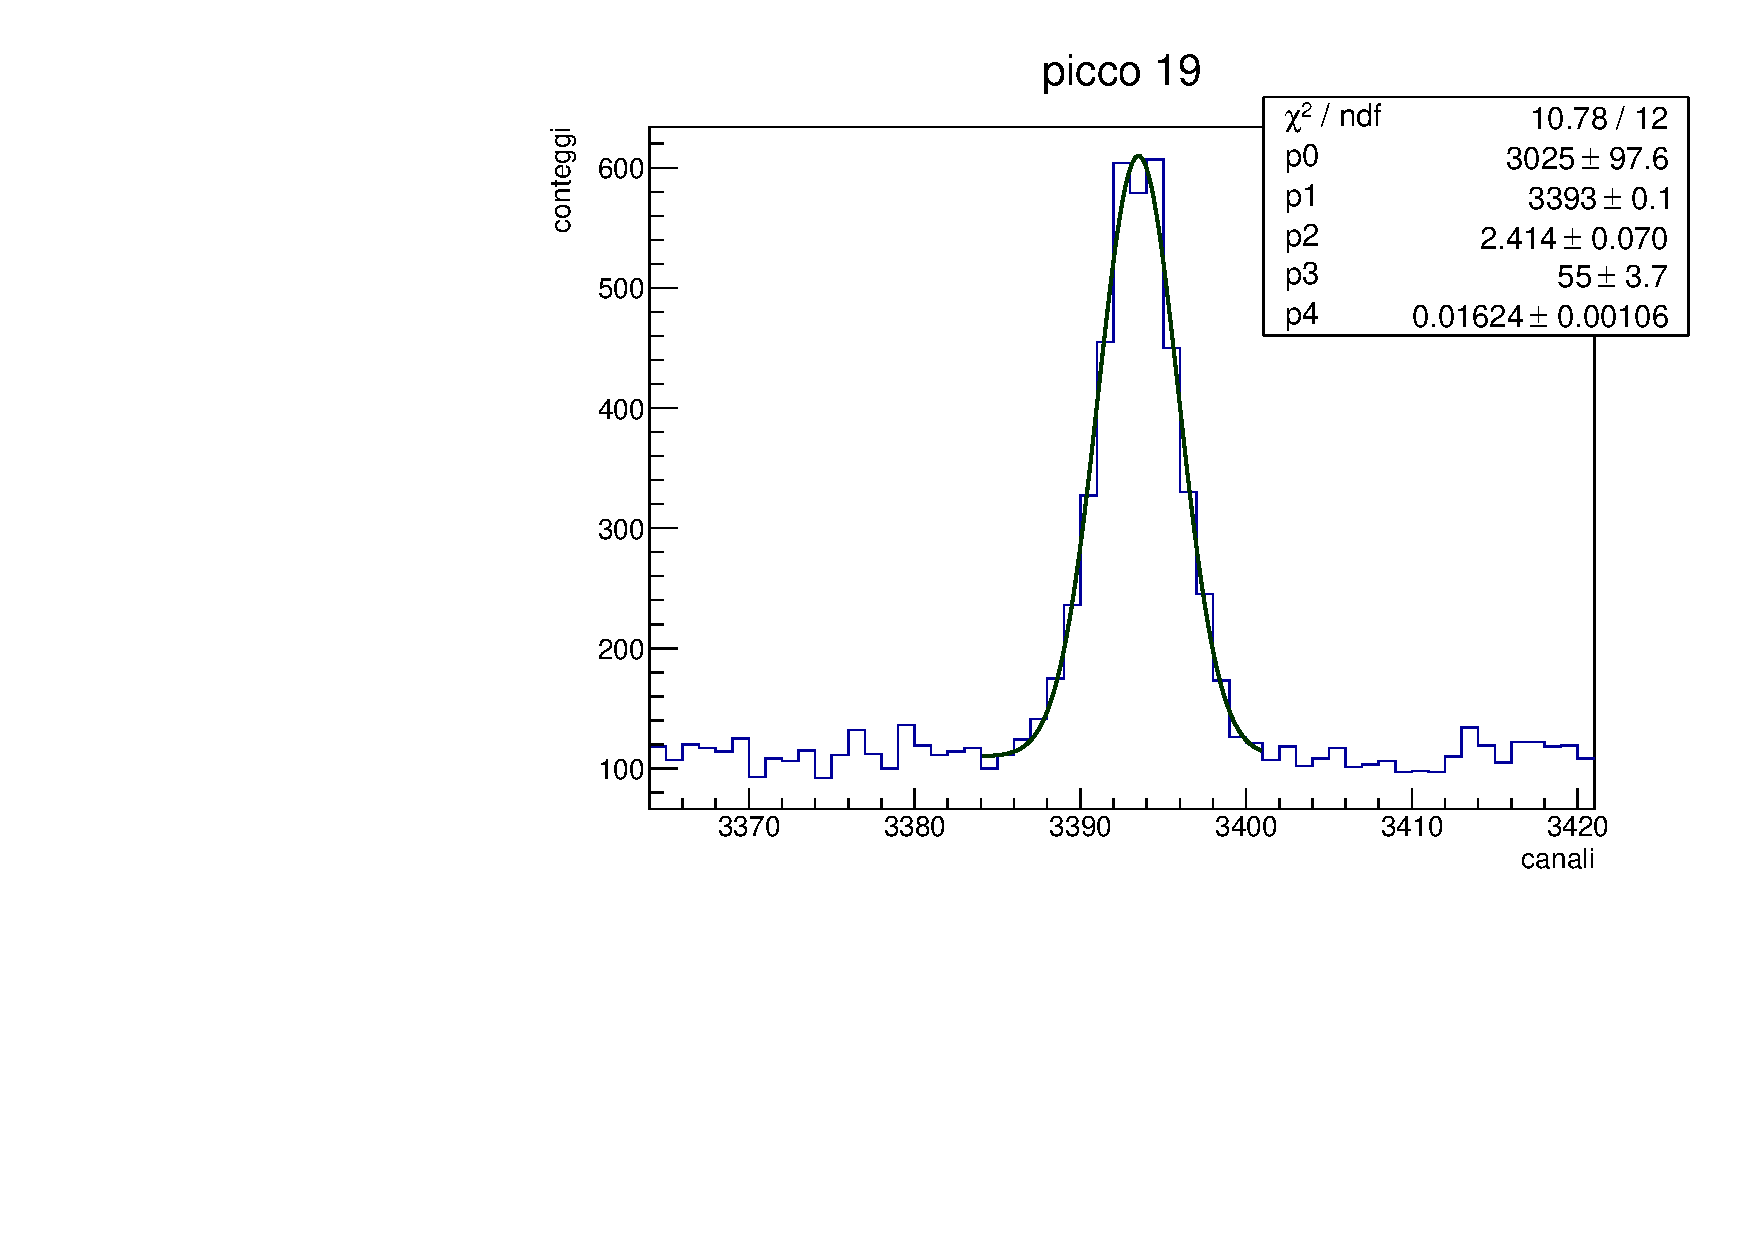
\includegraphics[width=2.2cm]{grafici/picco_incognita_germanio_19.pdf}
                    }
                \subfigure[picco 20]
                    {
                        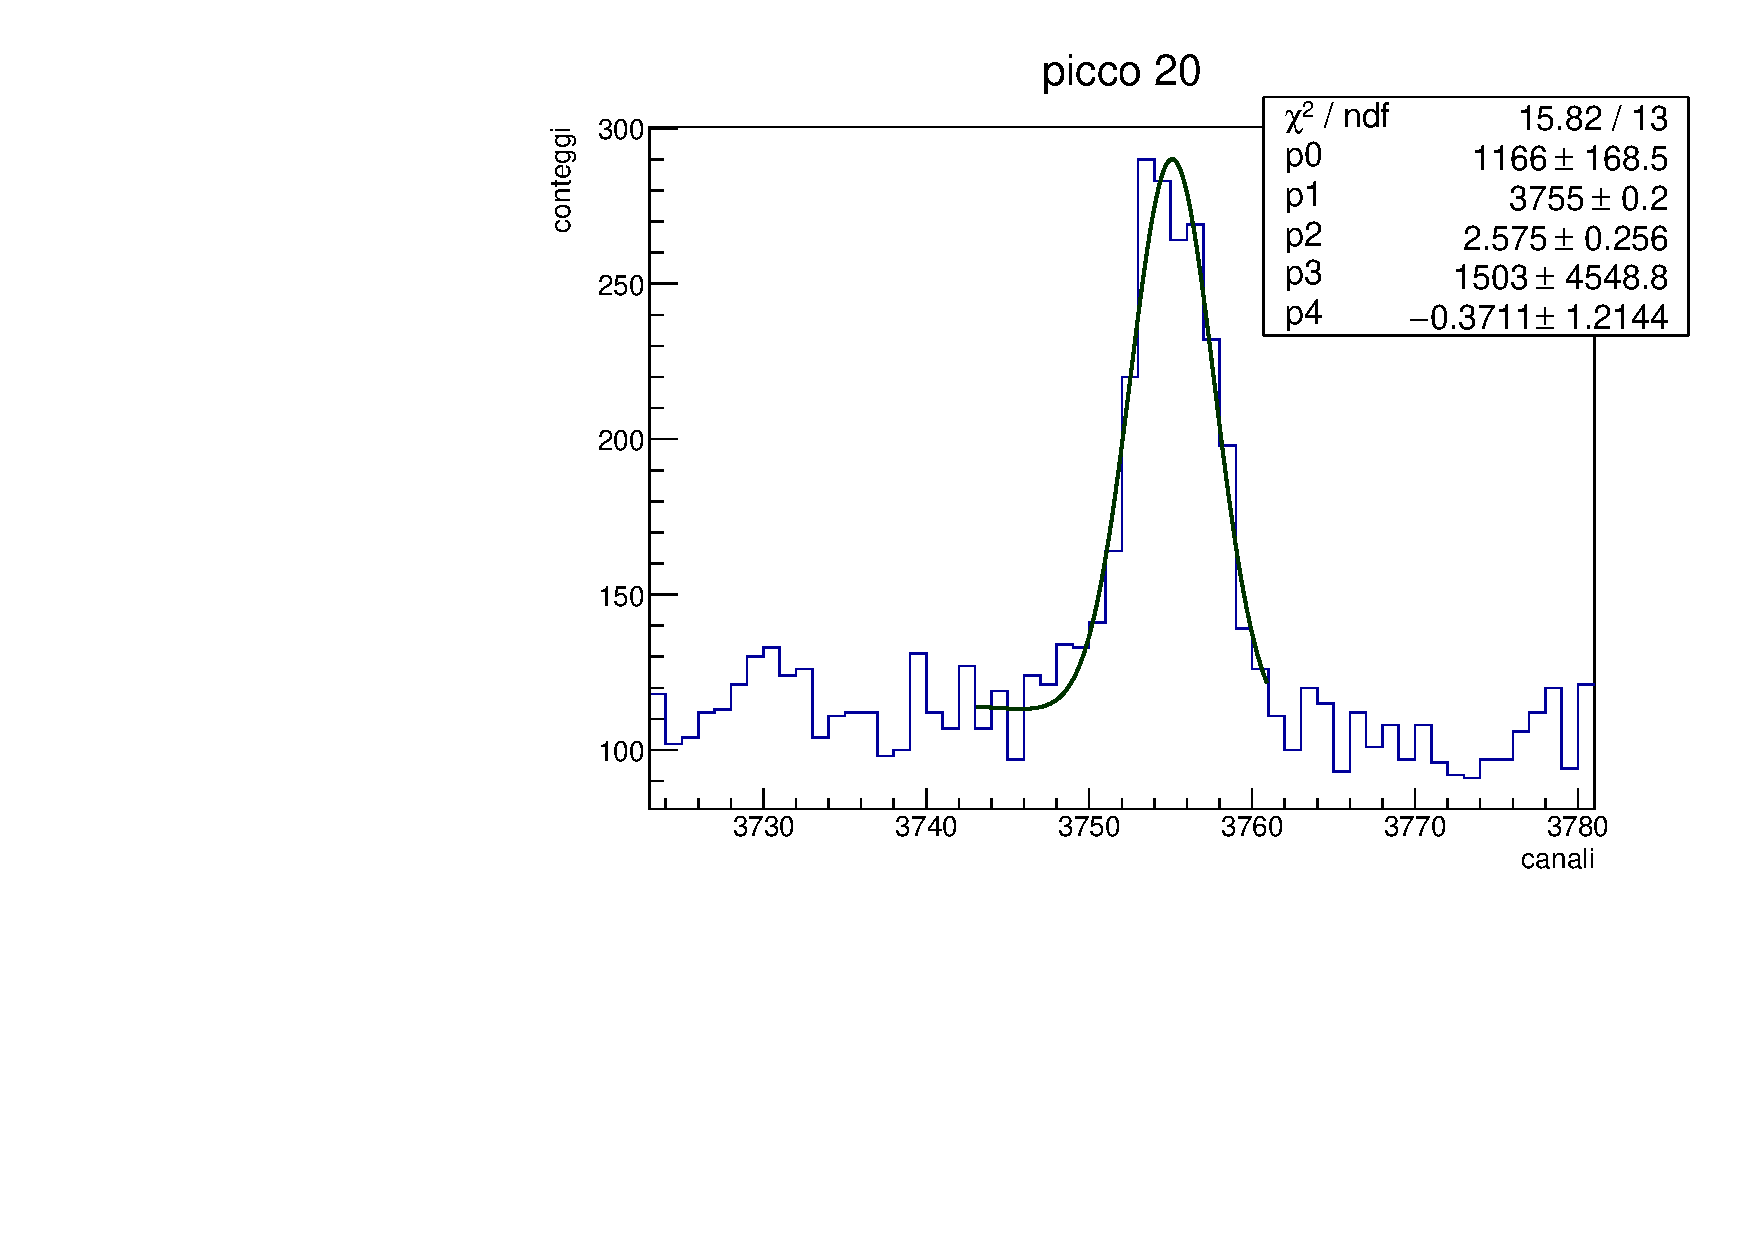
\includegraphics[width=2.2cm]{grafici/picco_incognita_germanio_20.pdf}
                    }

                \subfigure[picco 21]
                    {
                        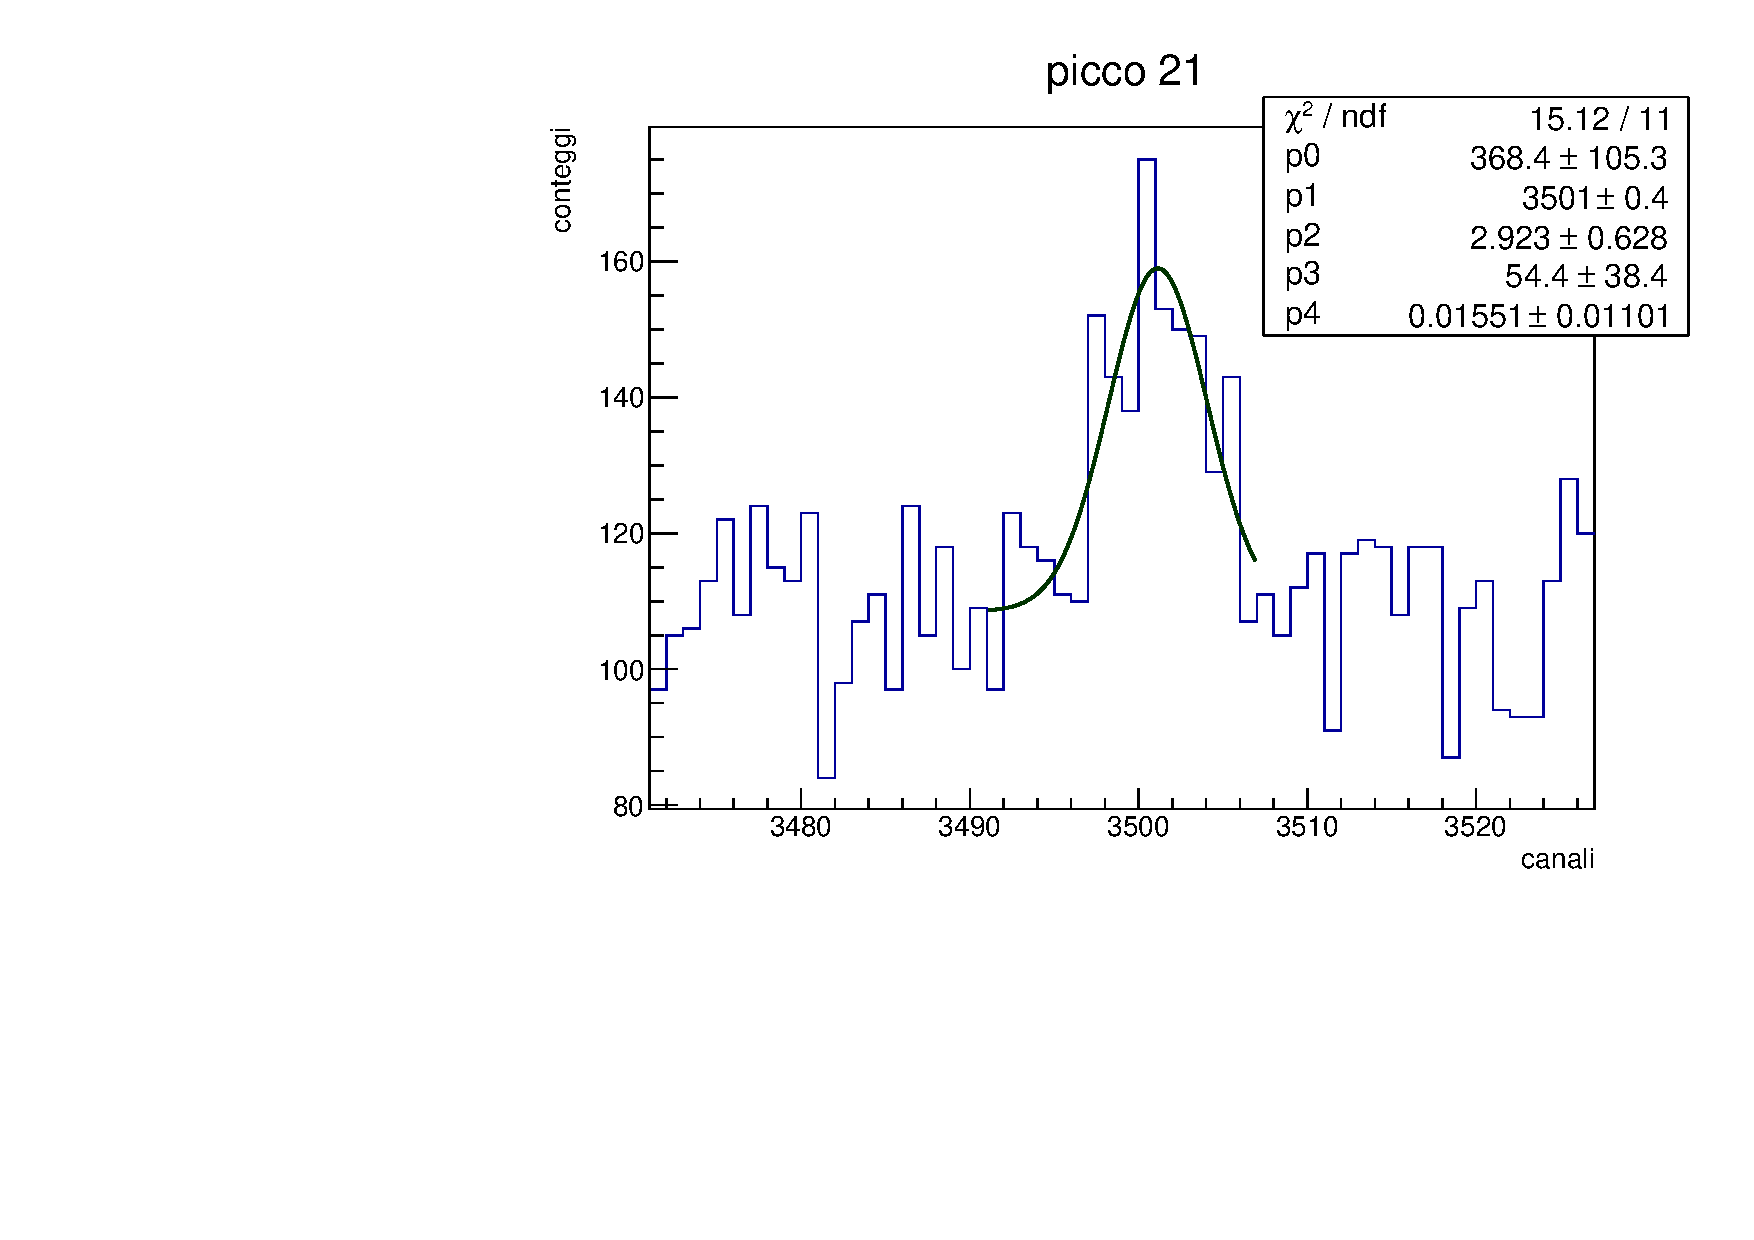
\includegraphics[width=2.2cm]{grafici/picco_incognita_germanio_21.pdf}
                    }
                \subfigure[picco 22]
                    {
                        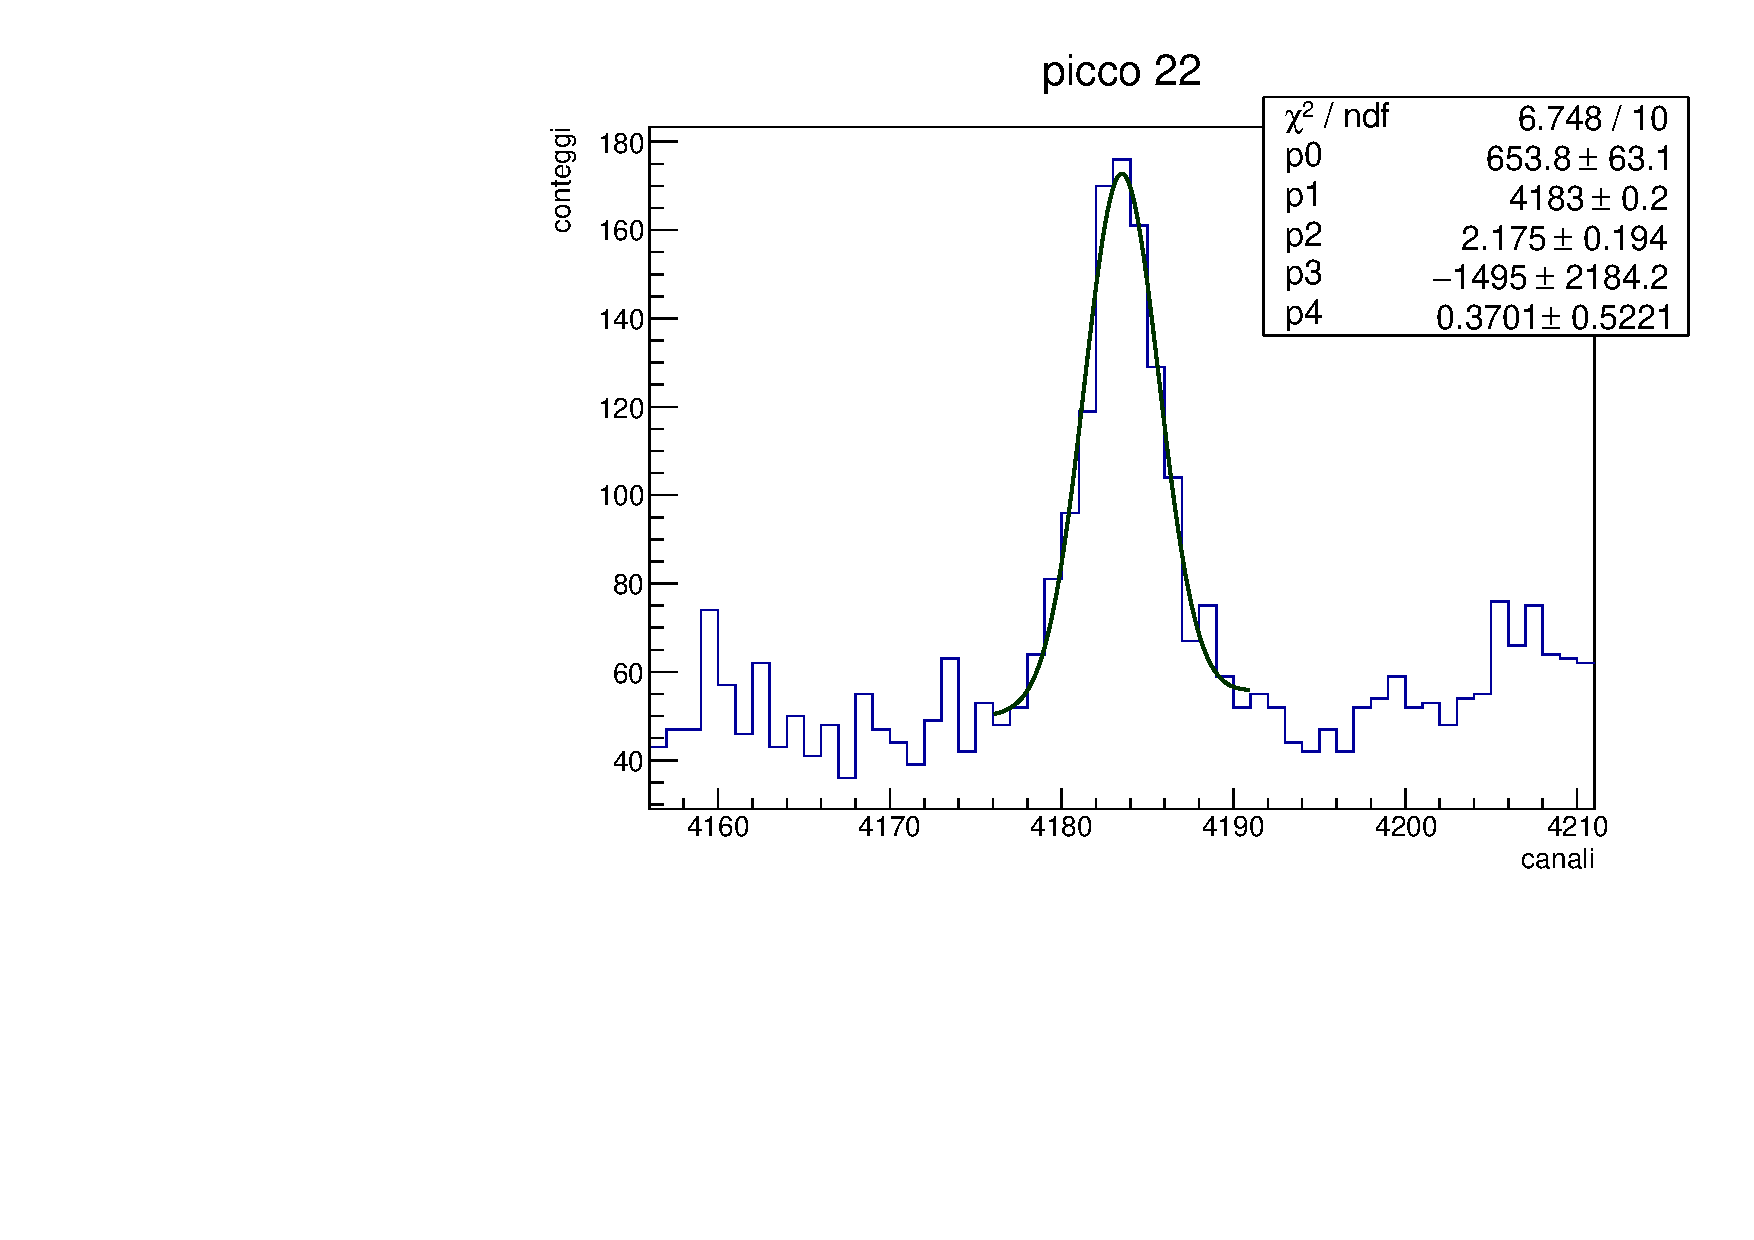
\includegraphics[width=2.2cm]{grafici/picco_incognita_germanio_22.pdf}
                    }
                \subfigure[picco 23]
                    {
                        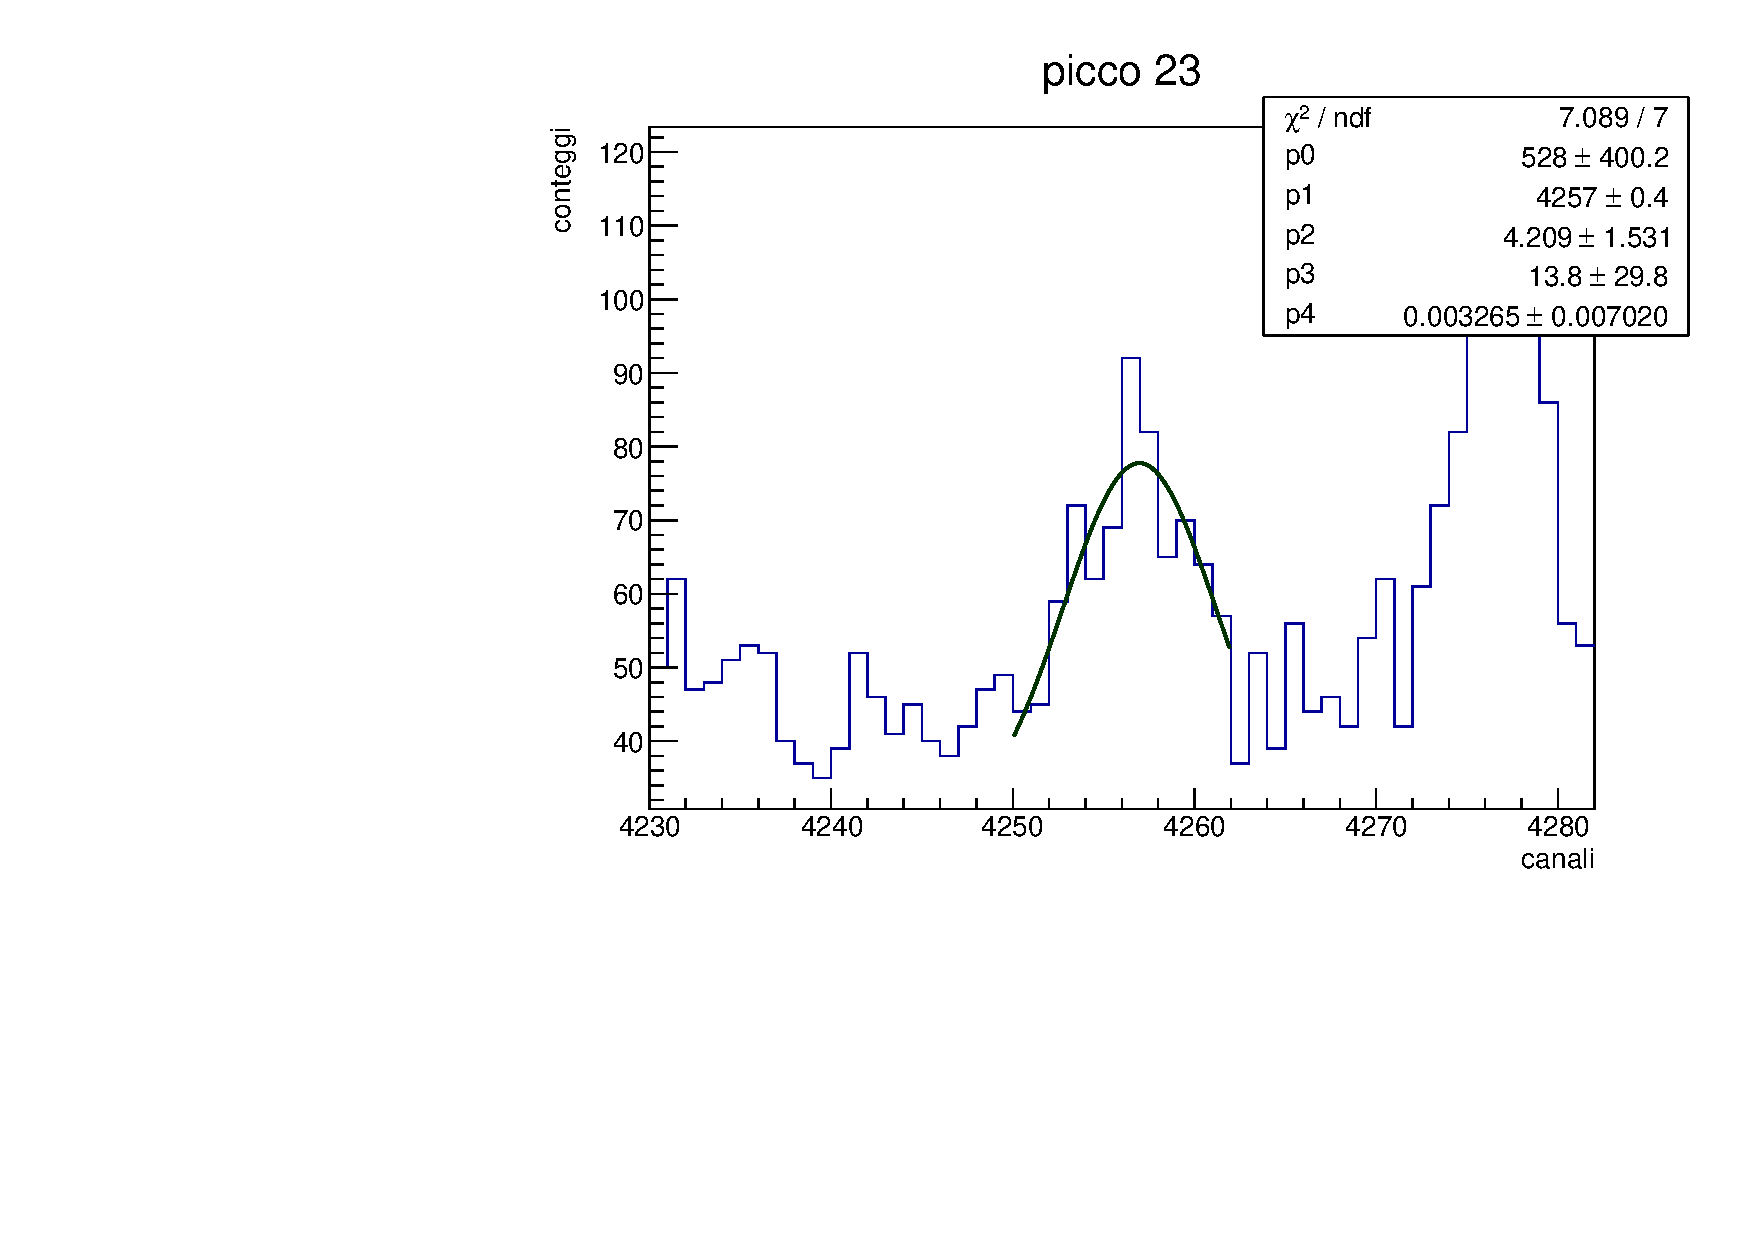
\includegraphics[width=2.2cm]{grafici/picco_incognita_germanio_23.pdf}
                    }
                \subfigure[picco 24]
                    {
                        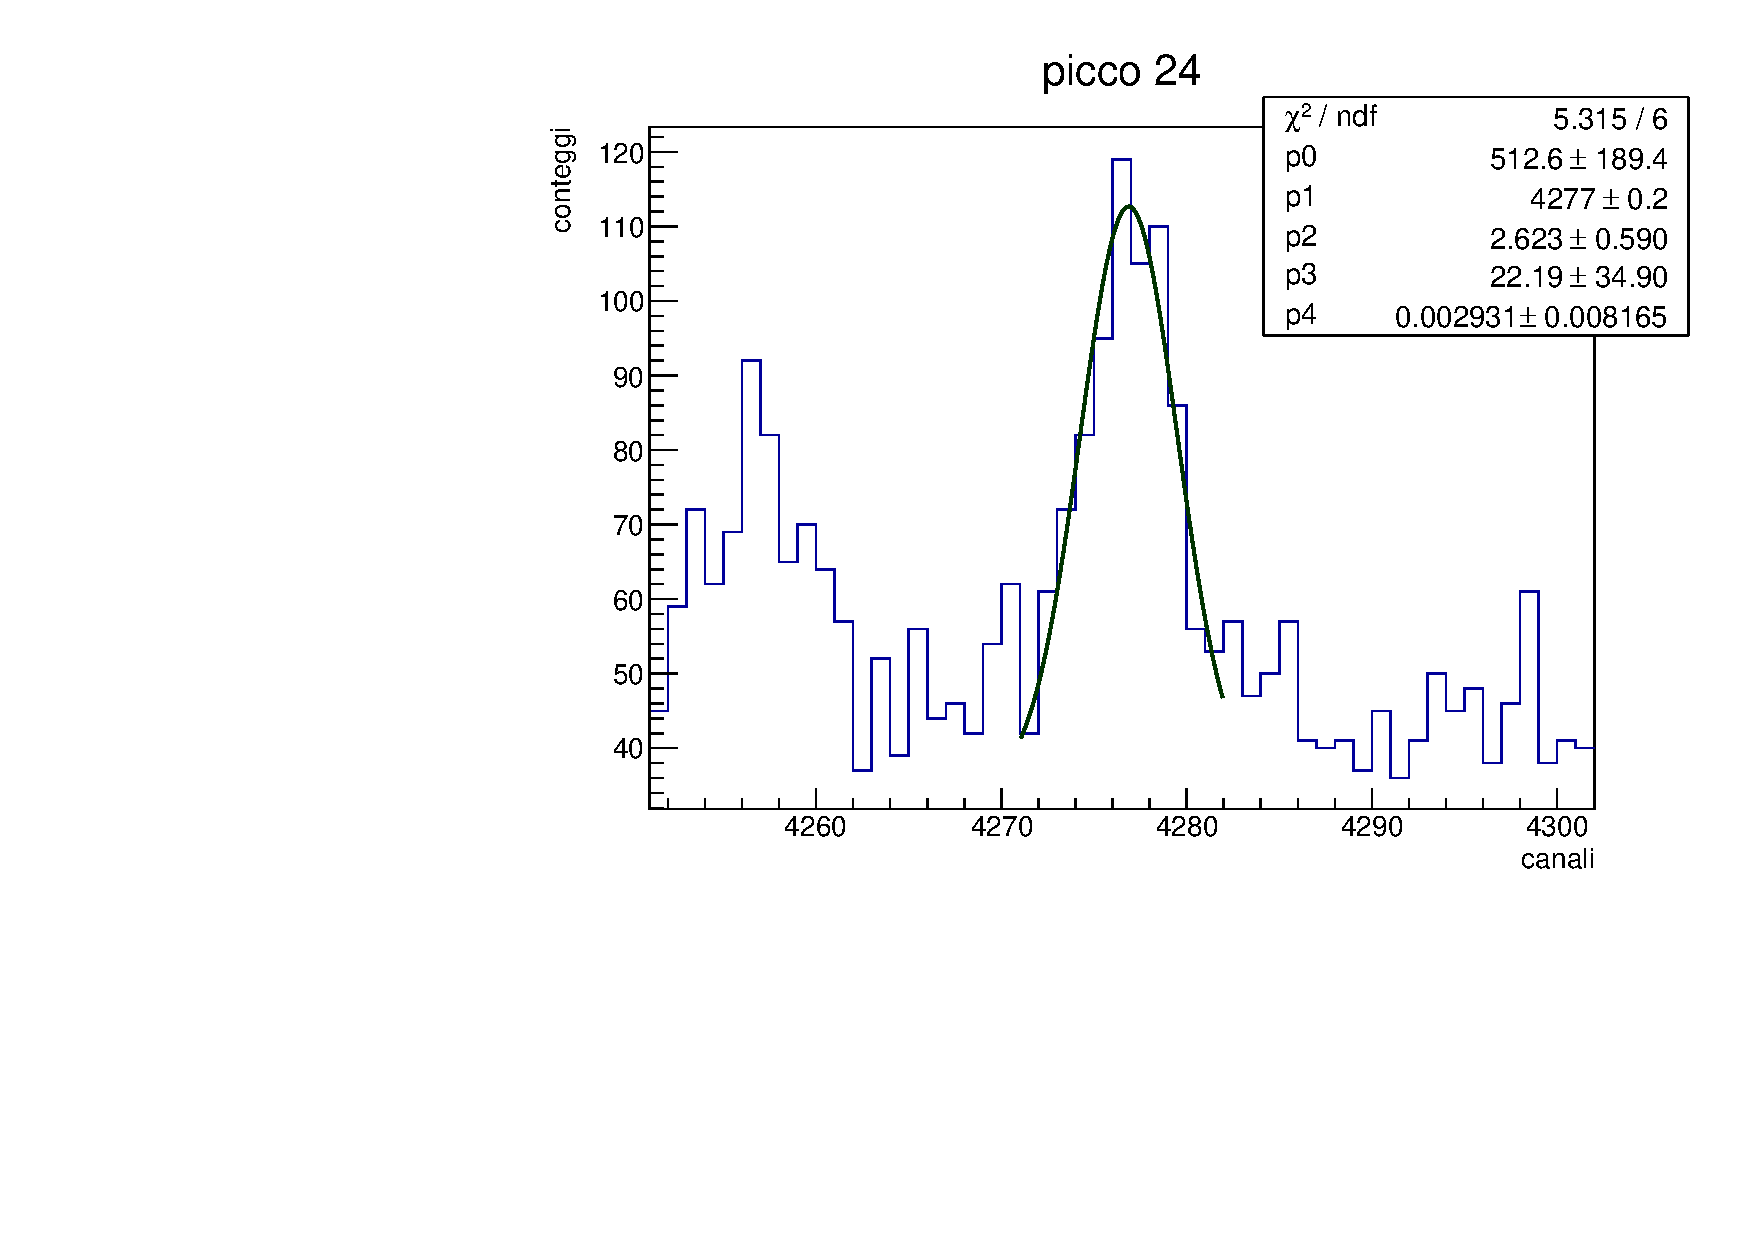
\includegraphics[width=2.2cm]{grafici/picco_incognita_germanio_24.pdf}
                    }
                \subfigure[picco 25]
                    {
                        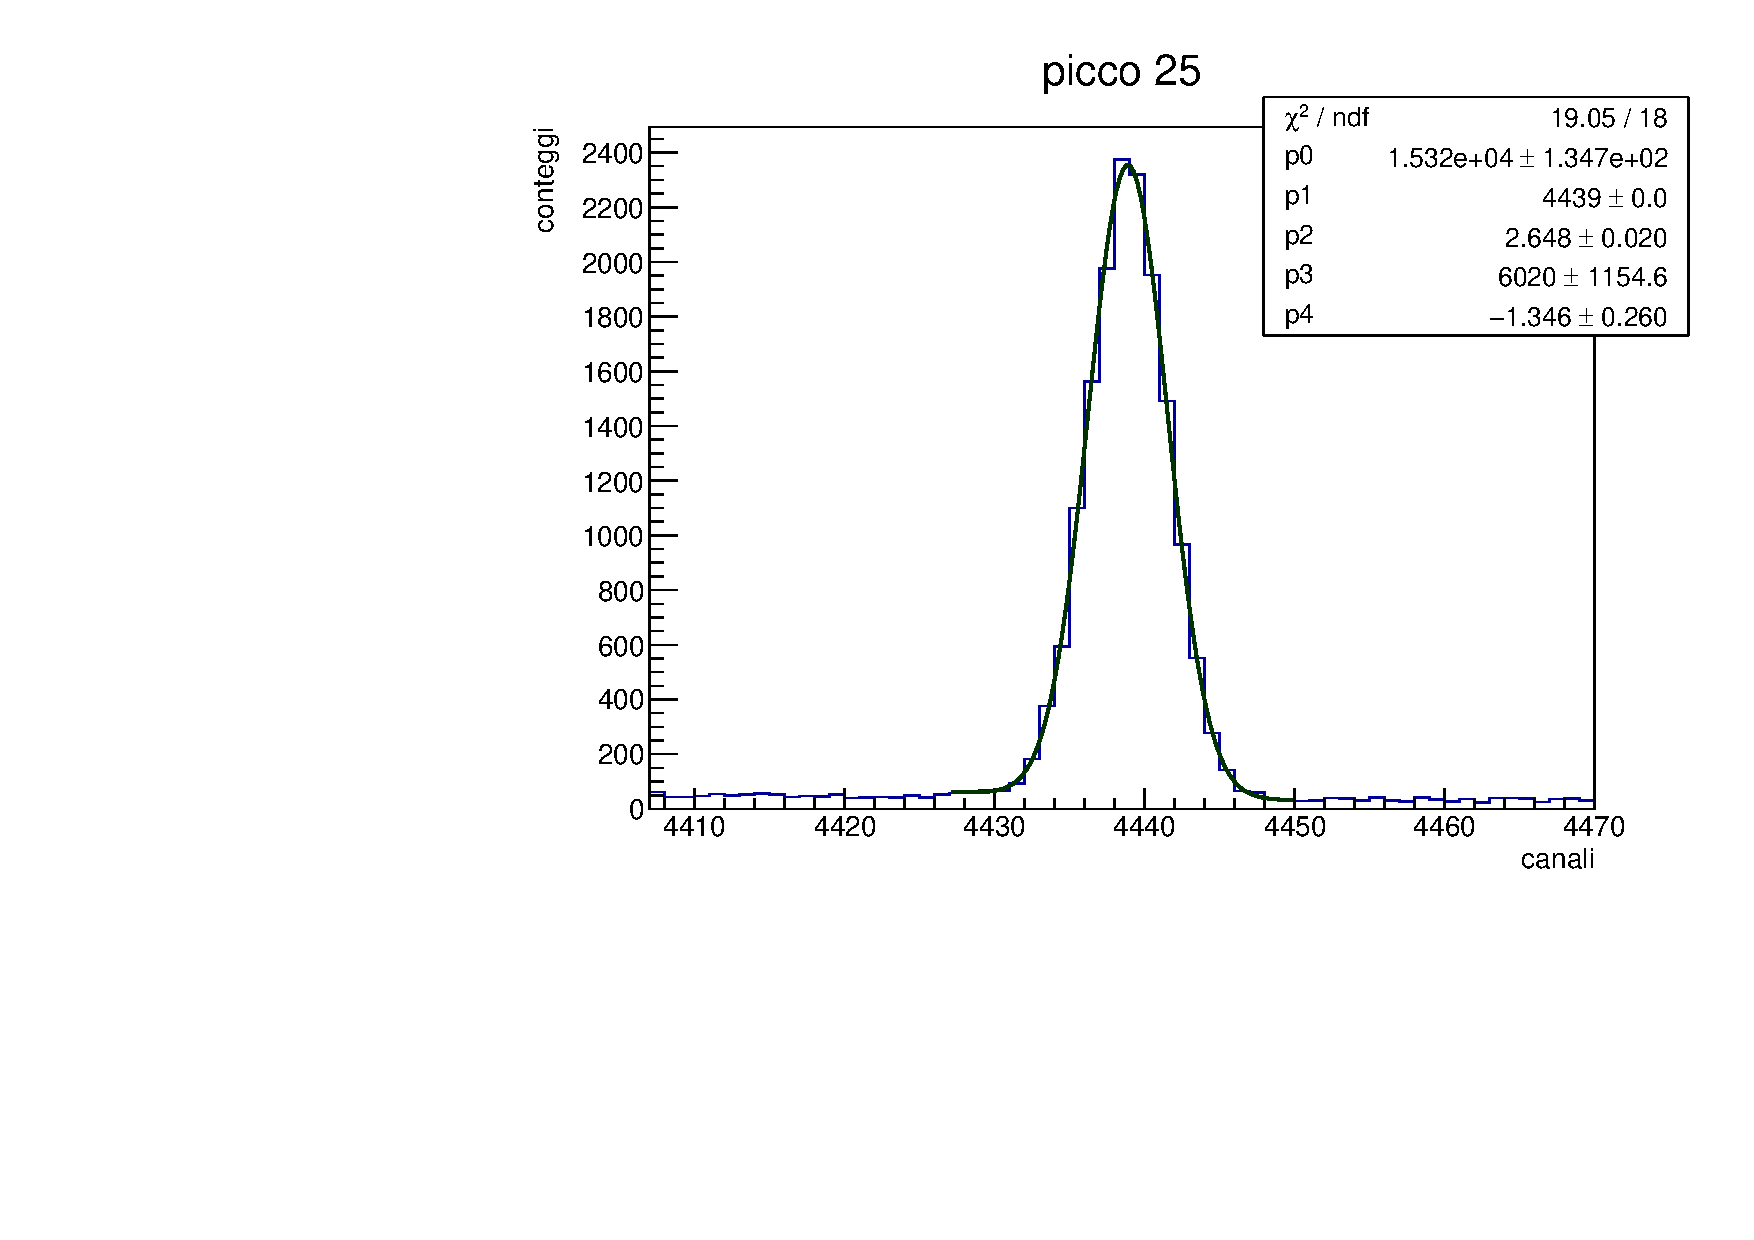
\includegraphics[width=2.2cm]{grafici/picco_incognita_germanio_25.pdf}
                    }
            \end{figure}
            \begin{figure}[h!]
                \centering
                \caption{picchi sorgente incognita con fit}
                \label{fig:picchi_incognita_germanio_2}
                \subfigure[picco 26]
                    {
                        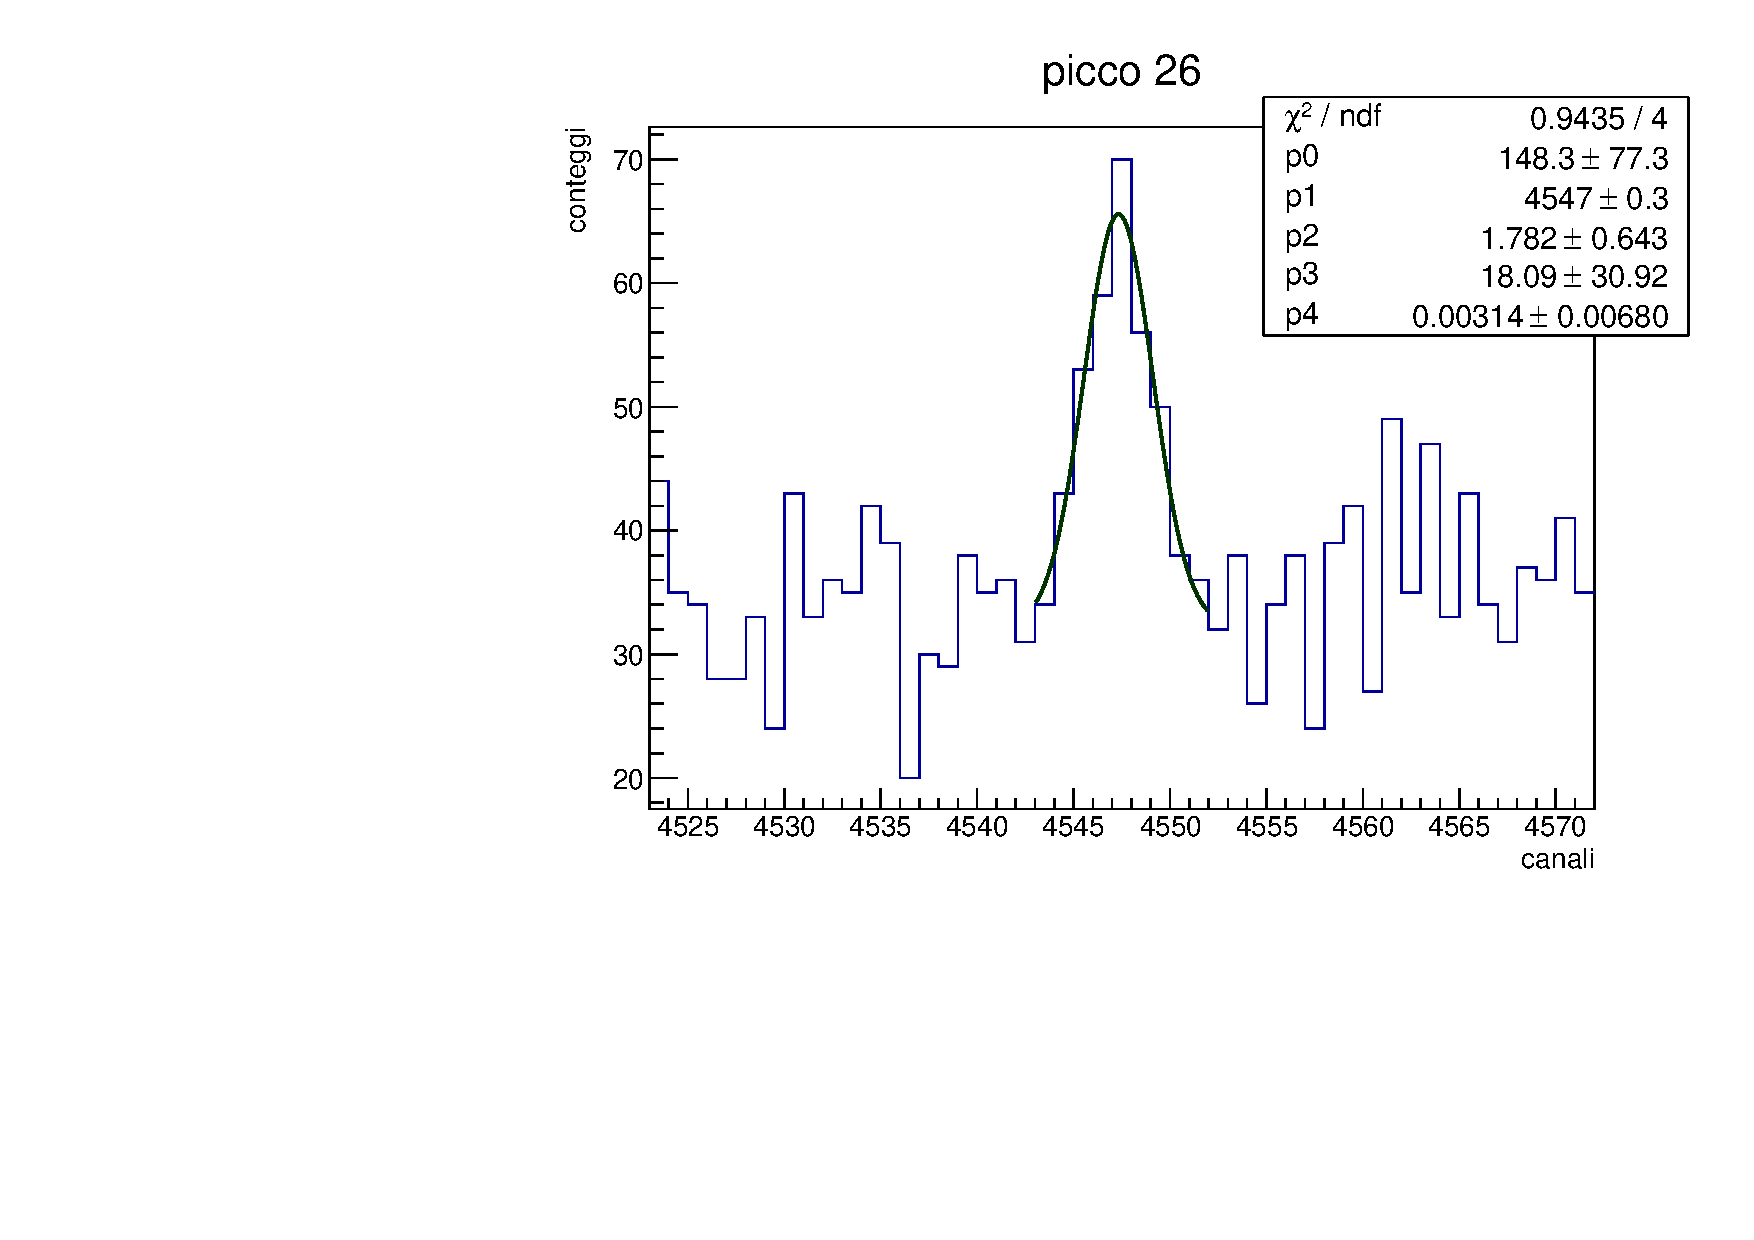
\includegraphics[width=2.2cm]{grafici/picco_incognita_germanio_26.pdf}
                    }
                \subfigure[picco 27]
                    {
                        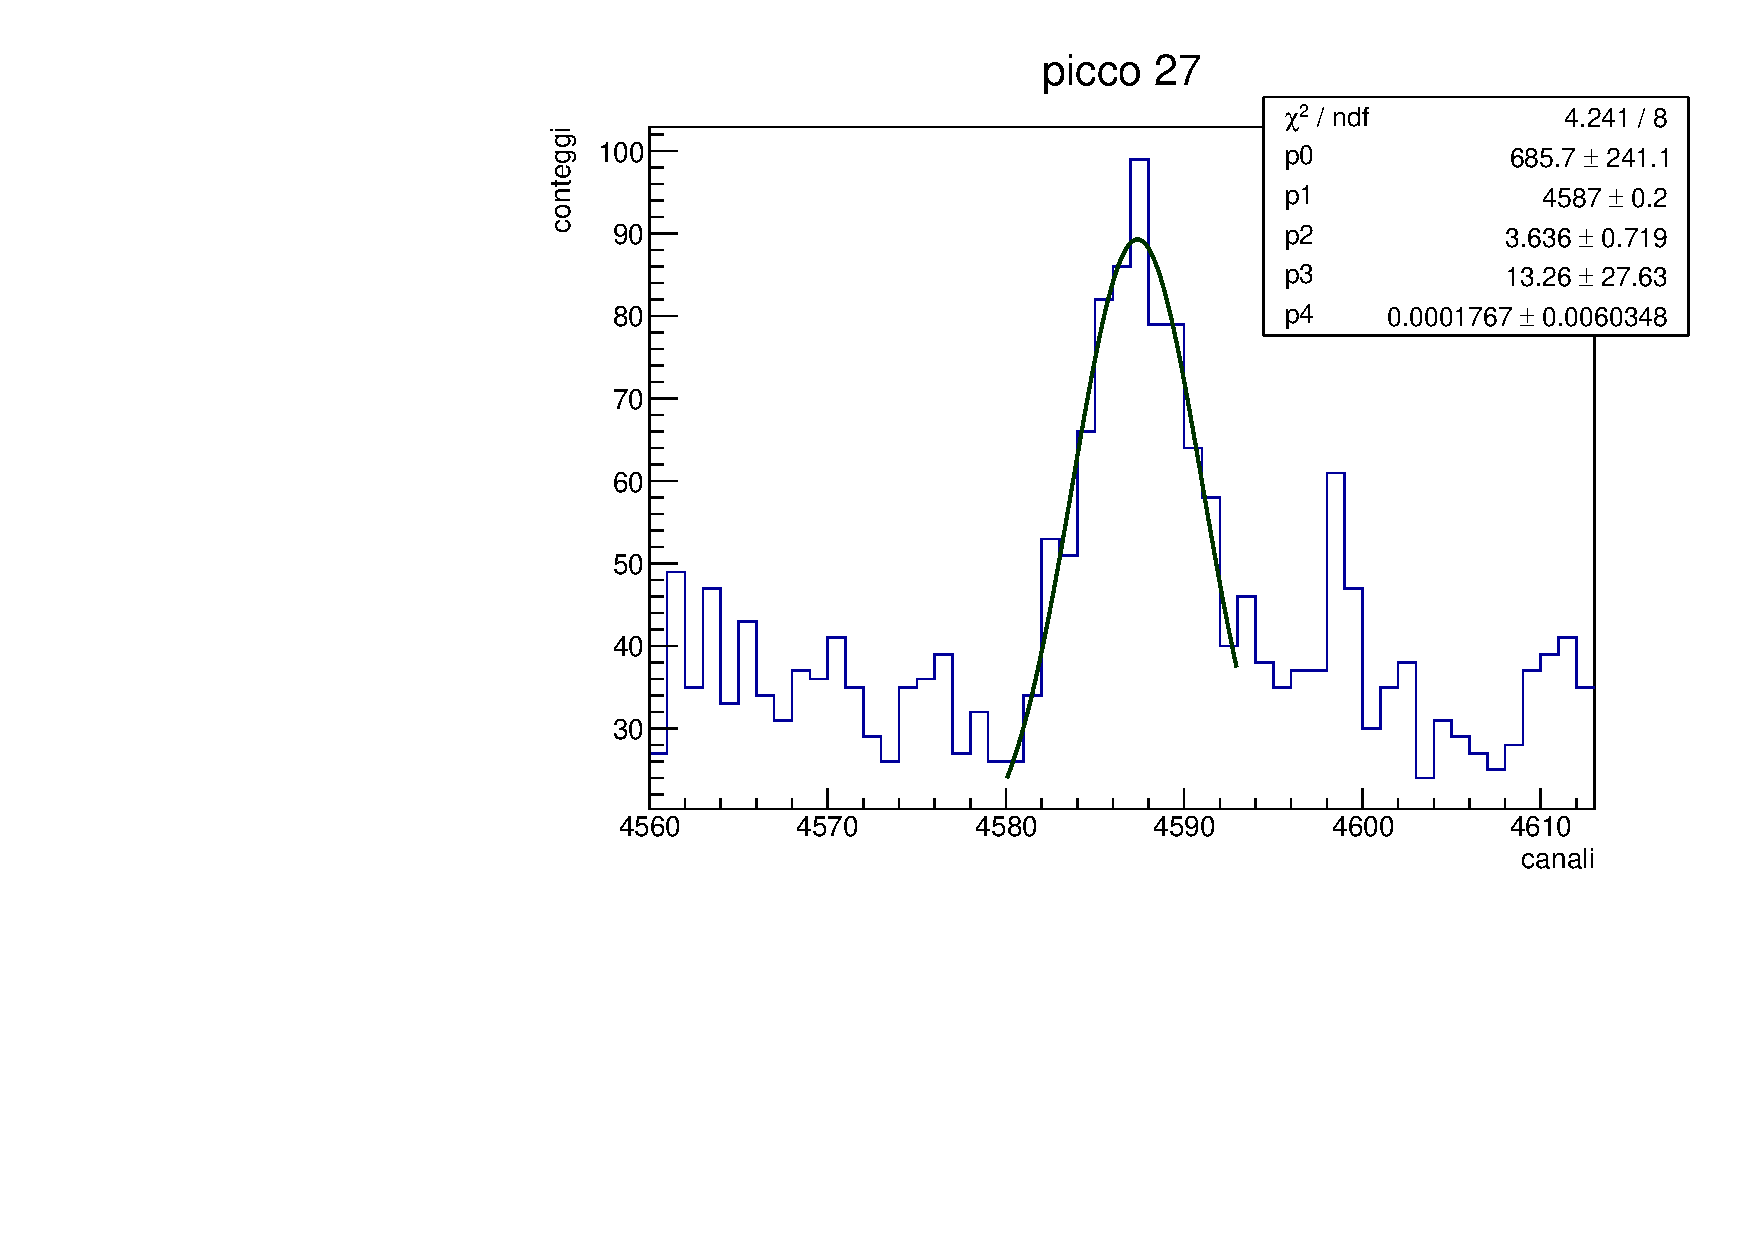
\includegraphics[width=2.2cm]{grafici/picco_incognita_germanio_27.pdf}
                    }
                \subfigure[picco 28]
                    {
                        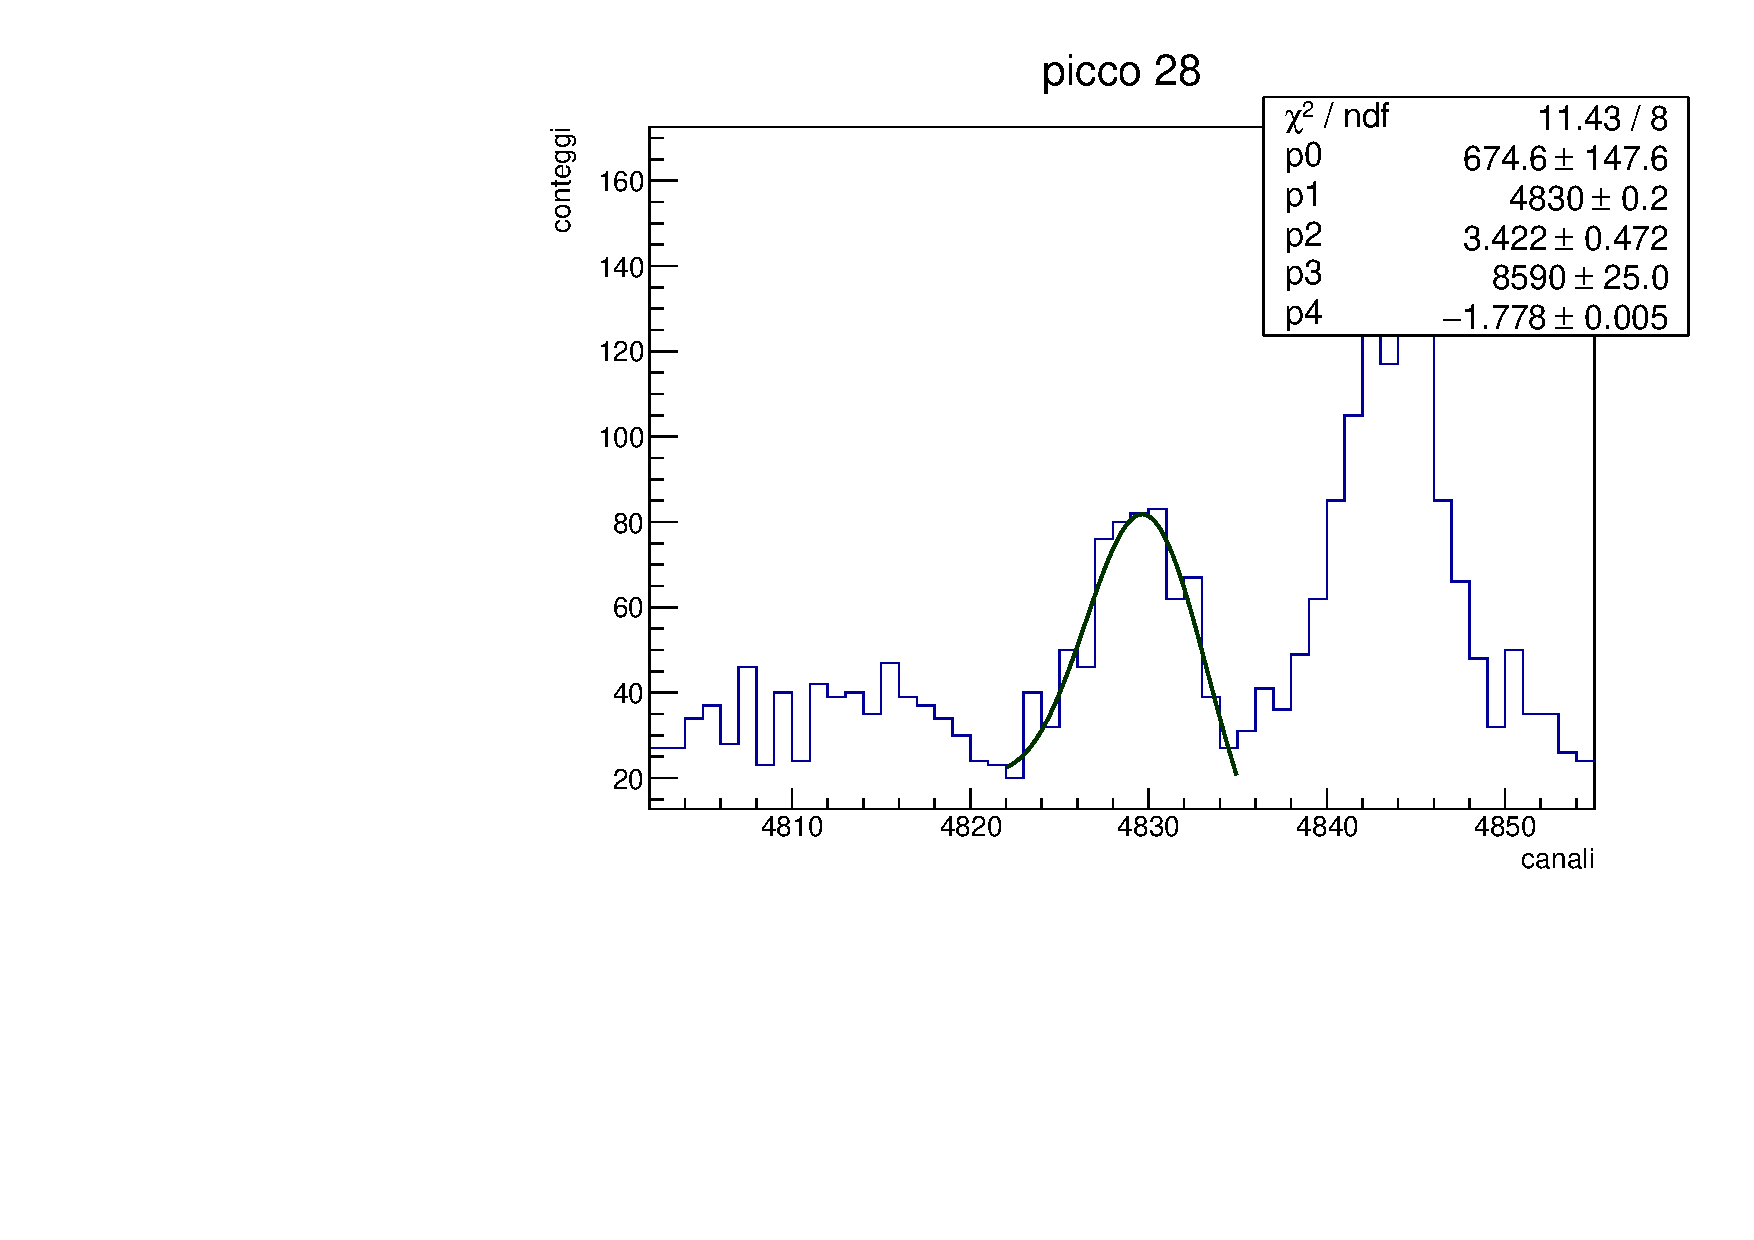
\includegraphics[width=2.2cm]{grafici/picco_incognita_germanio_28.pdf}
                    }
                \subfigure[picco 29]
                    {
                        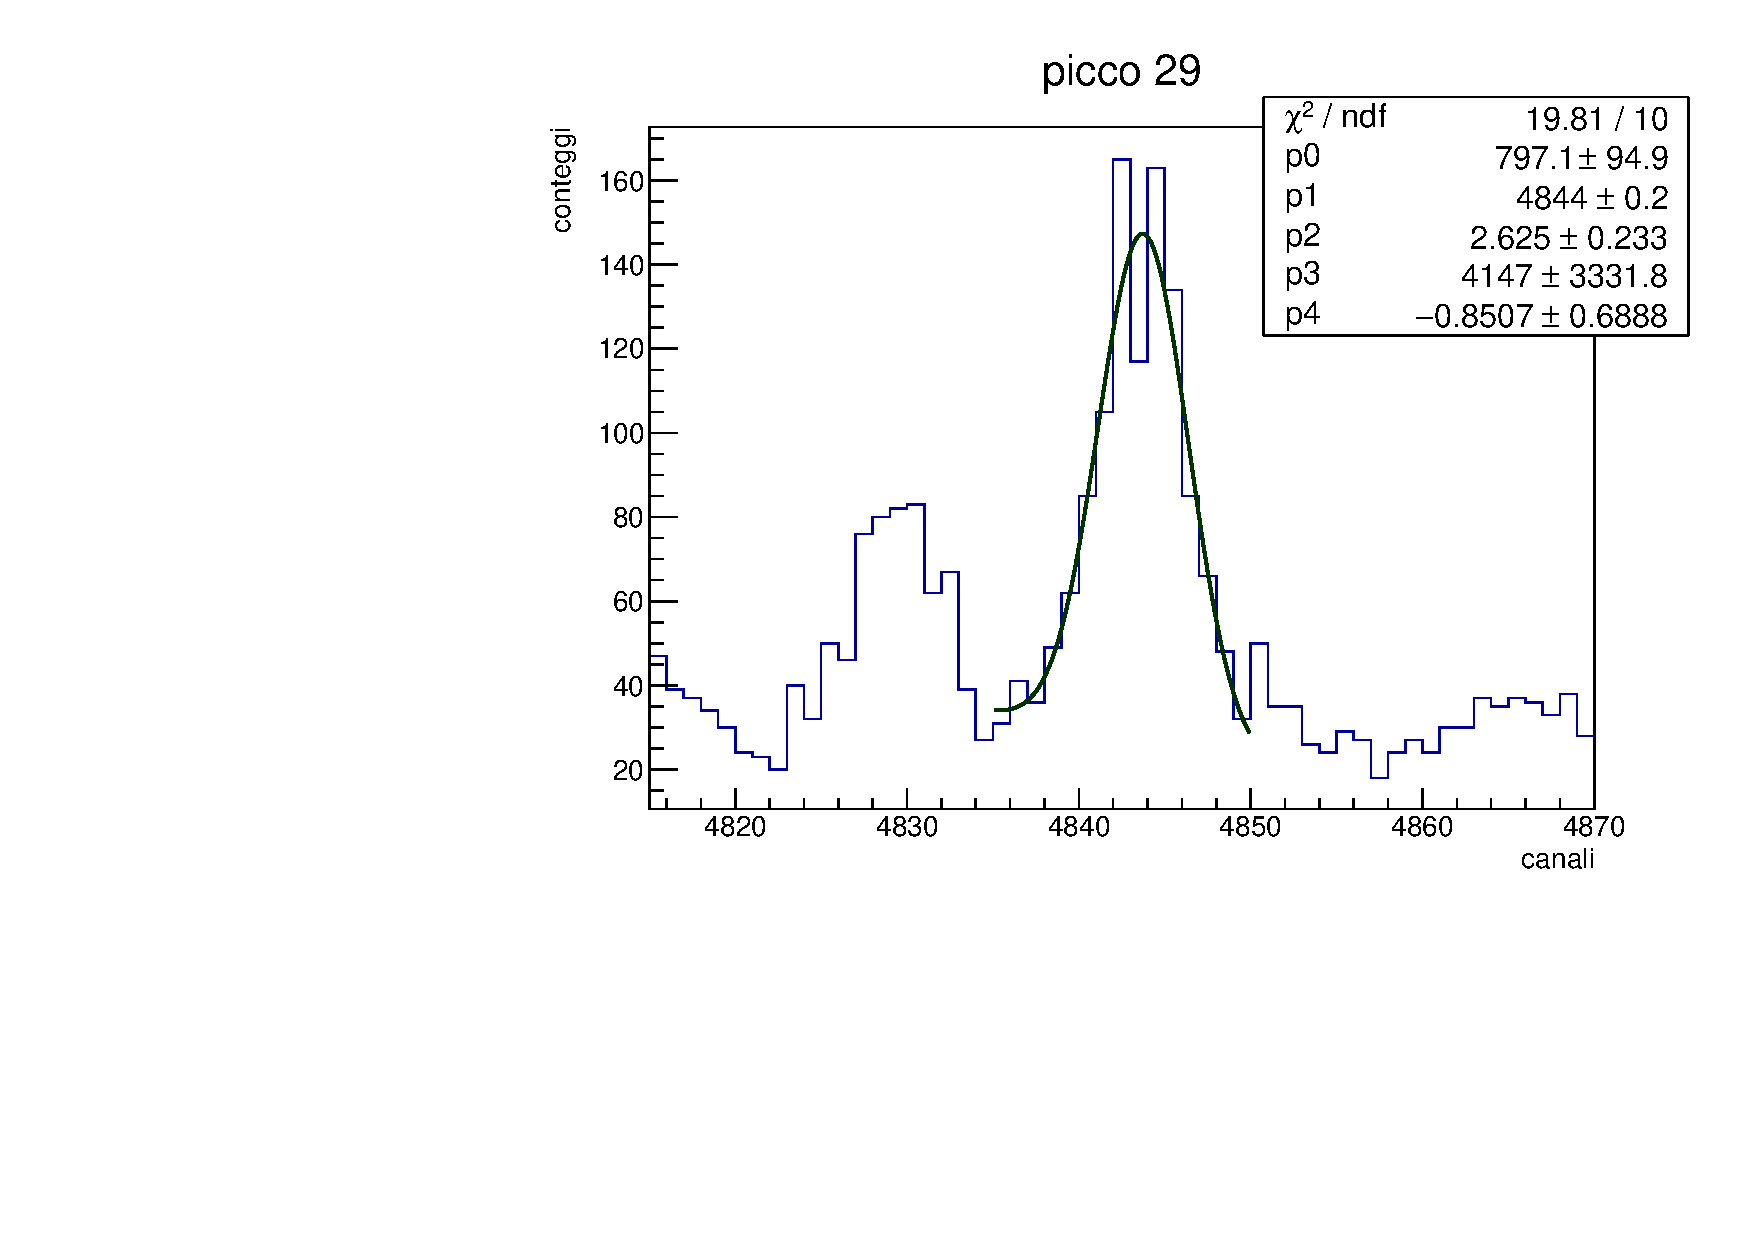
\includegraphics[width=2.2cm]{grafici/picco_incognita_germanio_29.pdf}
                    }
                \subfigure[picco 30]
                    {
                        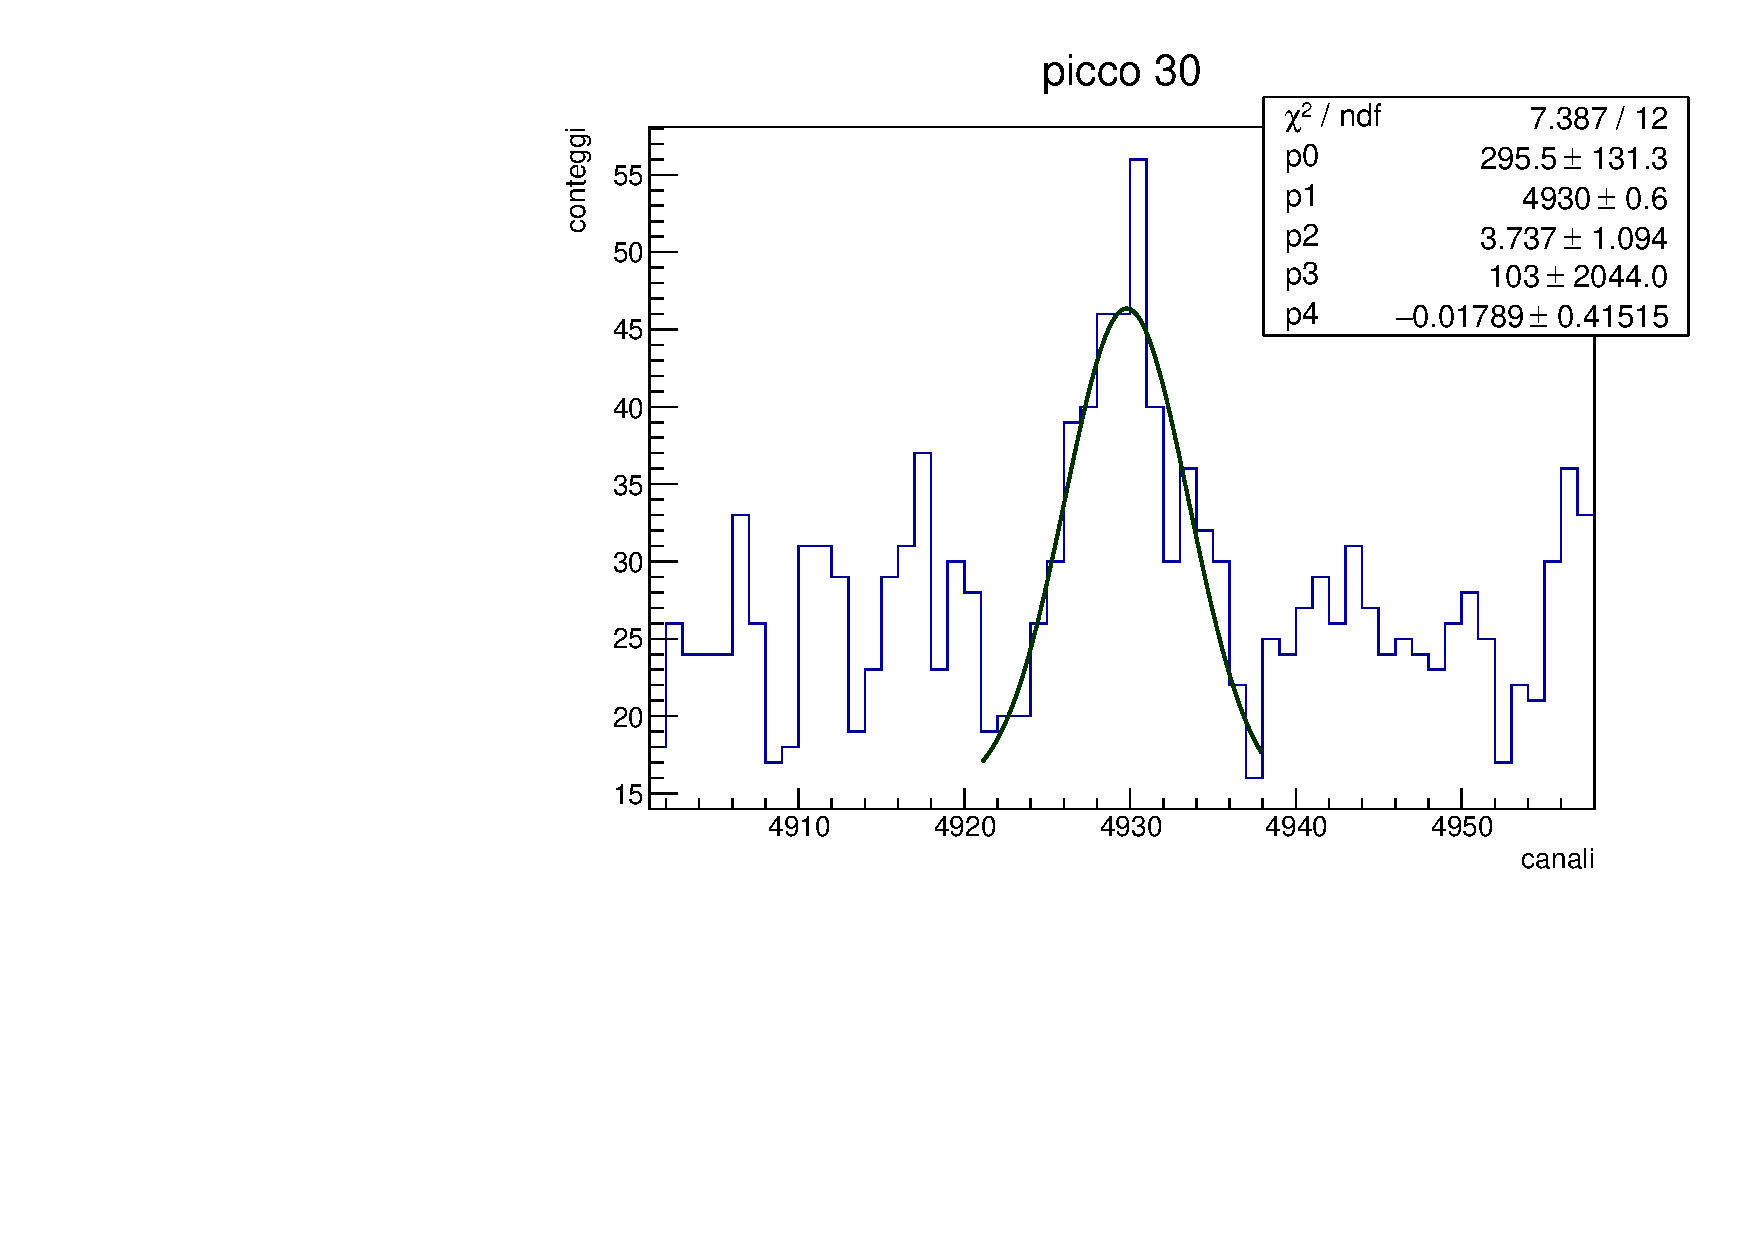
\includegraphics[width=2.2cm]{grafici/picco_incognita_germanio_30.pdf}
                    }

                \subfigure[picco 31]
                    {
                        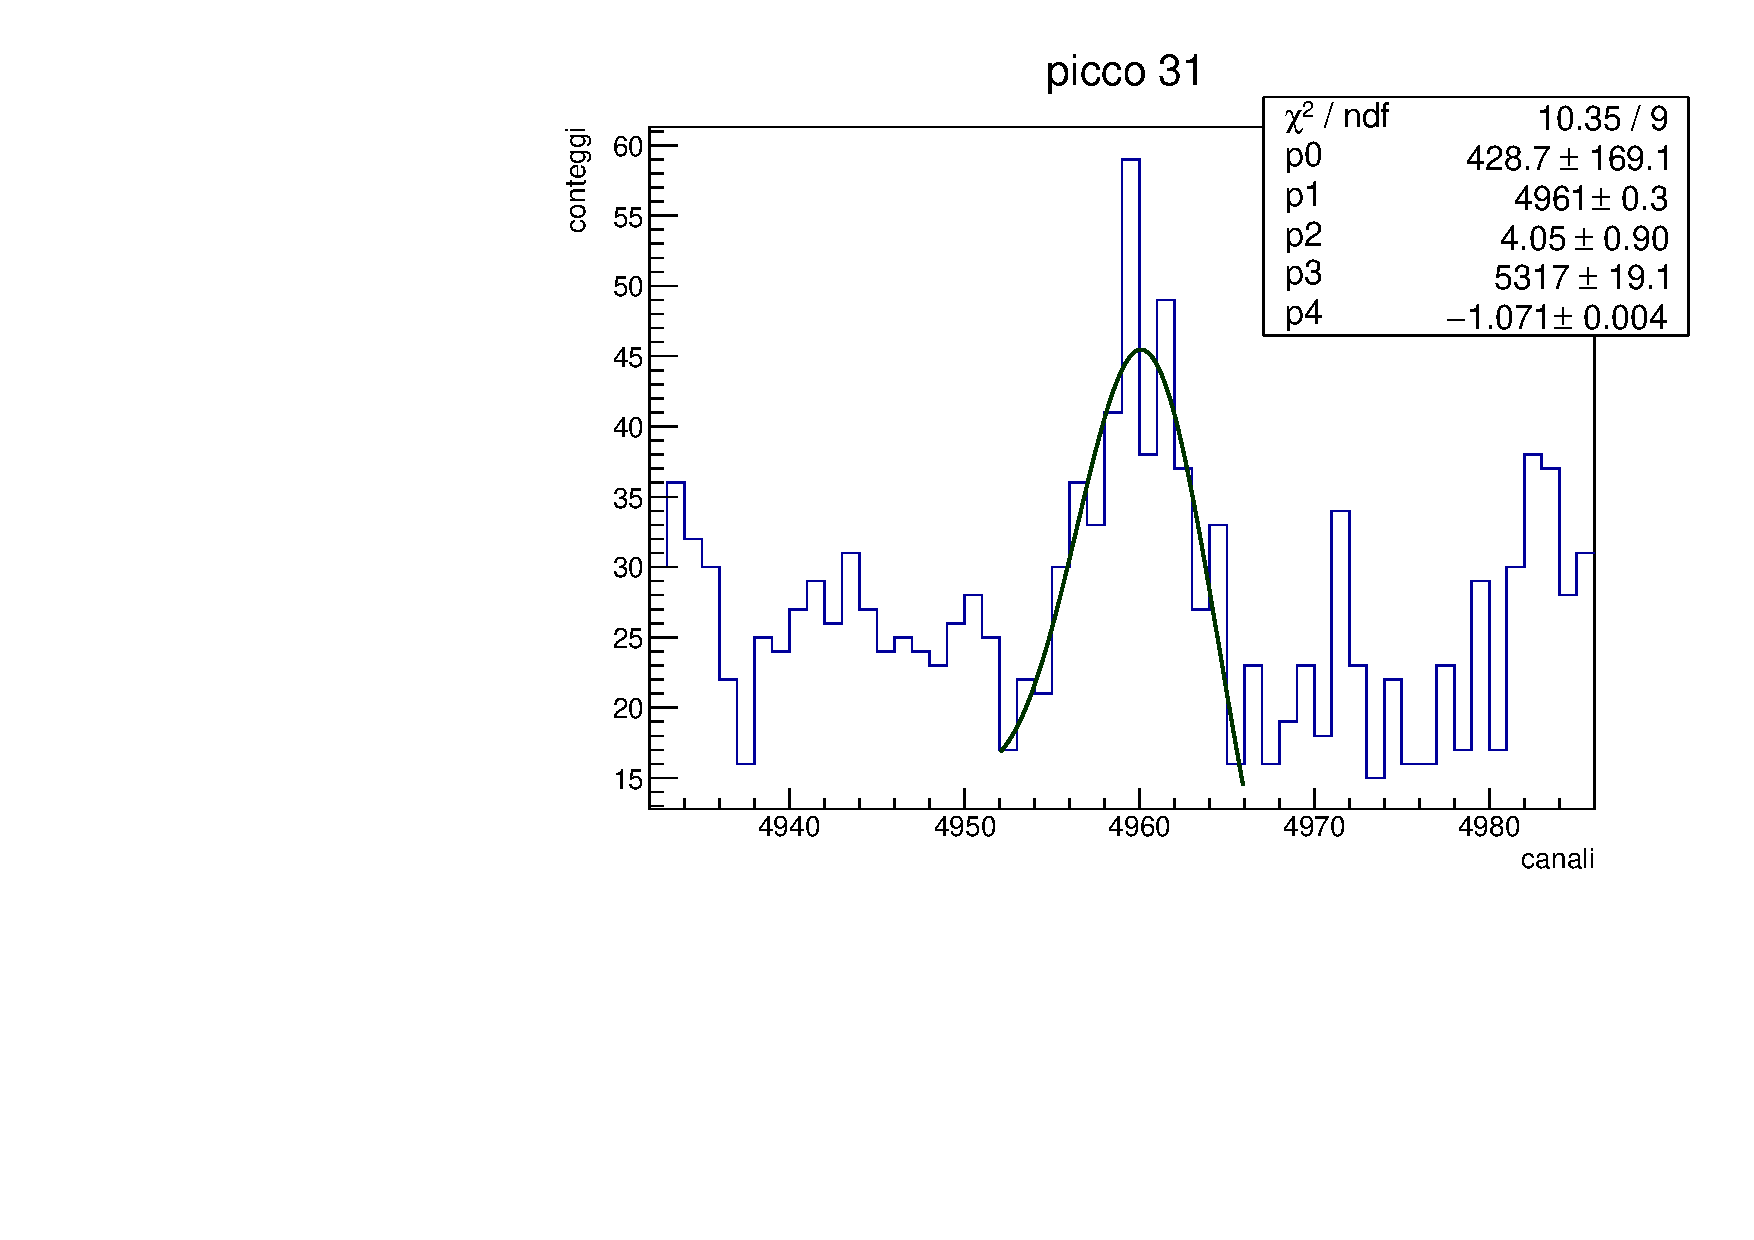
\includegraphics[width=2.2cm]{grafici/picco_incognita_germanio_31.pdf}
                    }
                \subfigure[picco 32]
                    {
                        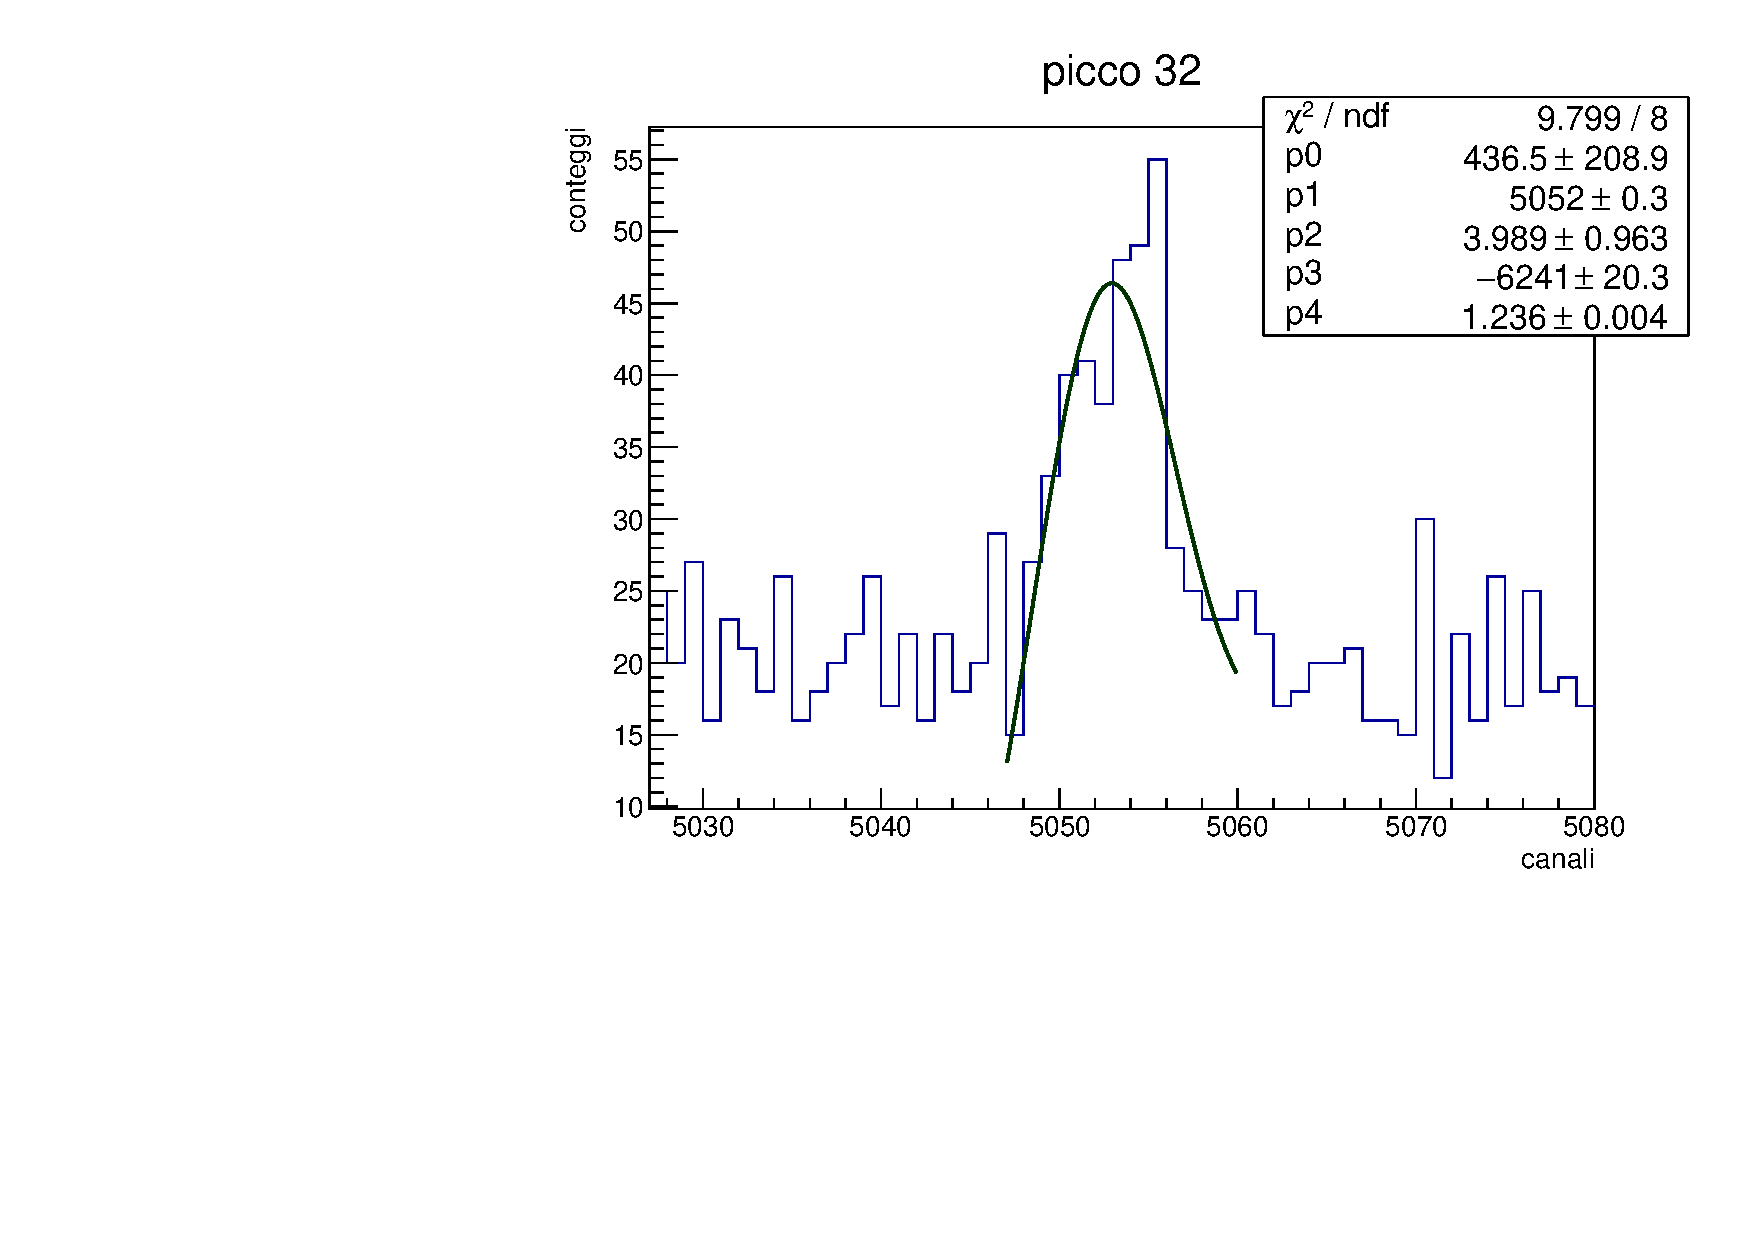
\includegraphics[width=2.2cm]{grafici/picco_incognita_germanio_32.pdf}
                    }
                \subfigure[picco 33]
                    {
                        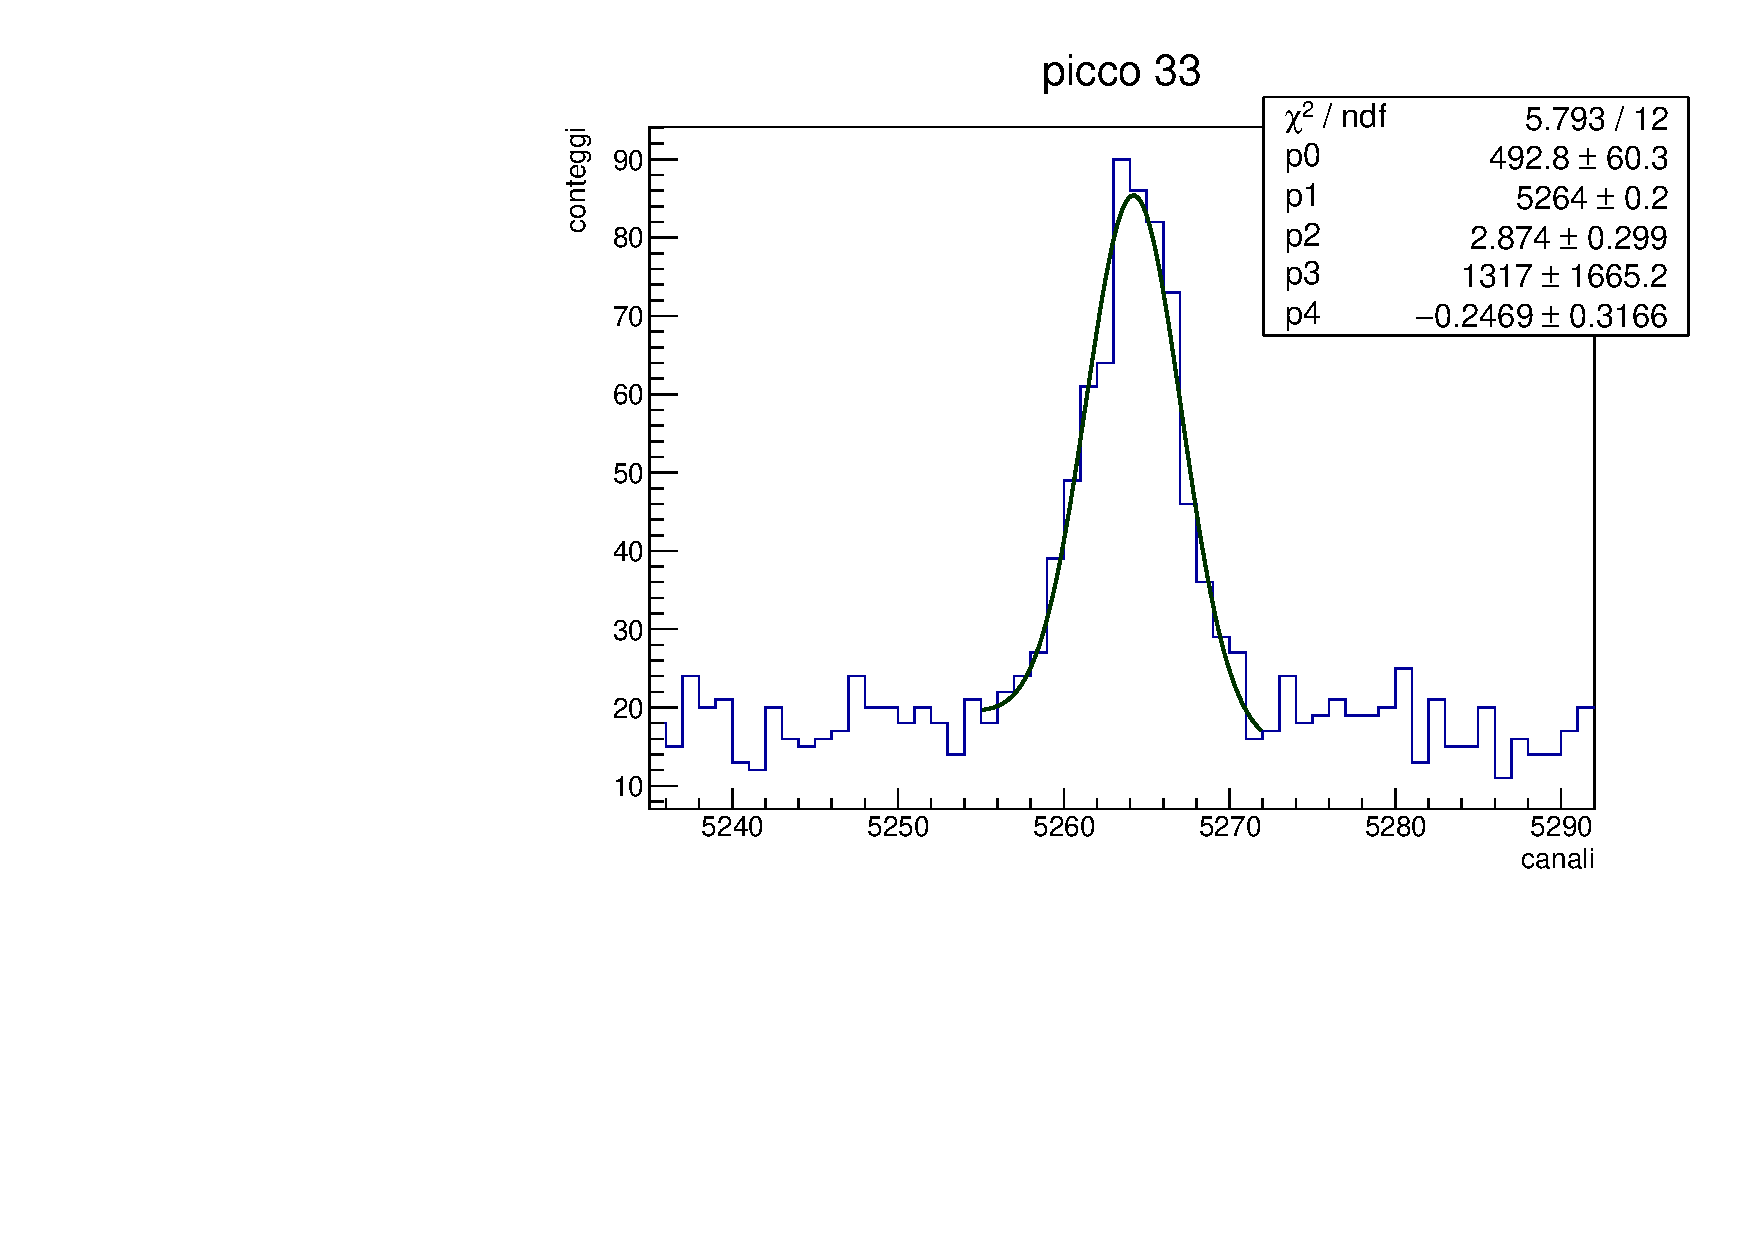
\includegraphics[width=2.2cm]{grafici/picco_incognita_germanio_33.pdf}
                    }
                \subfigure[picco 34]
                    {
                        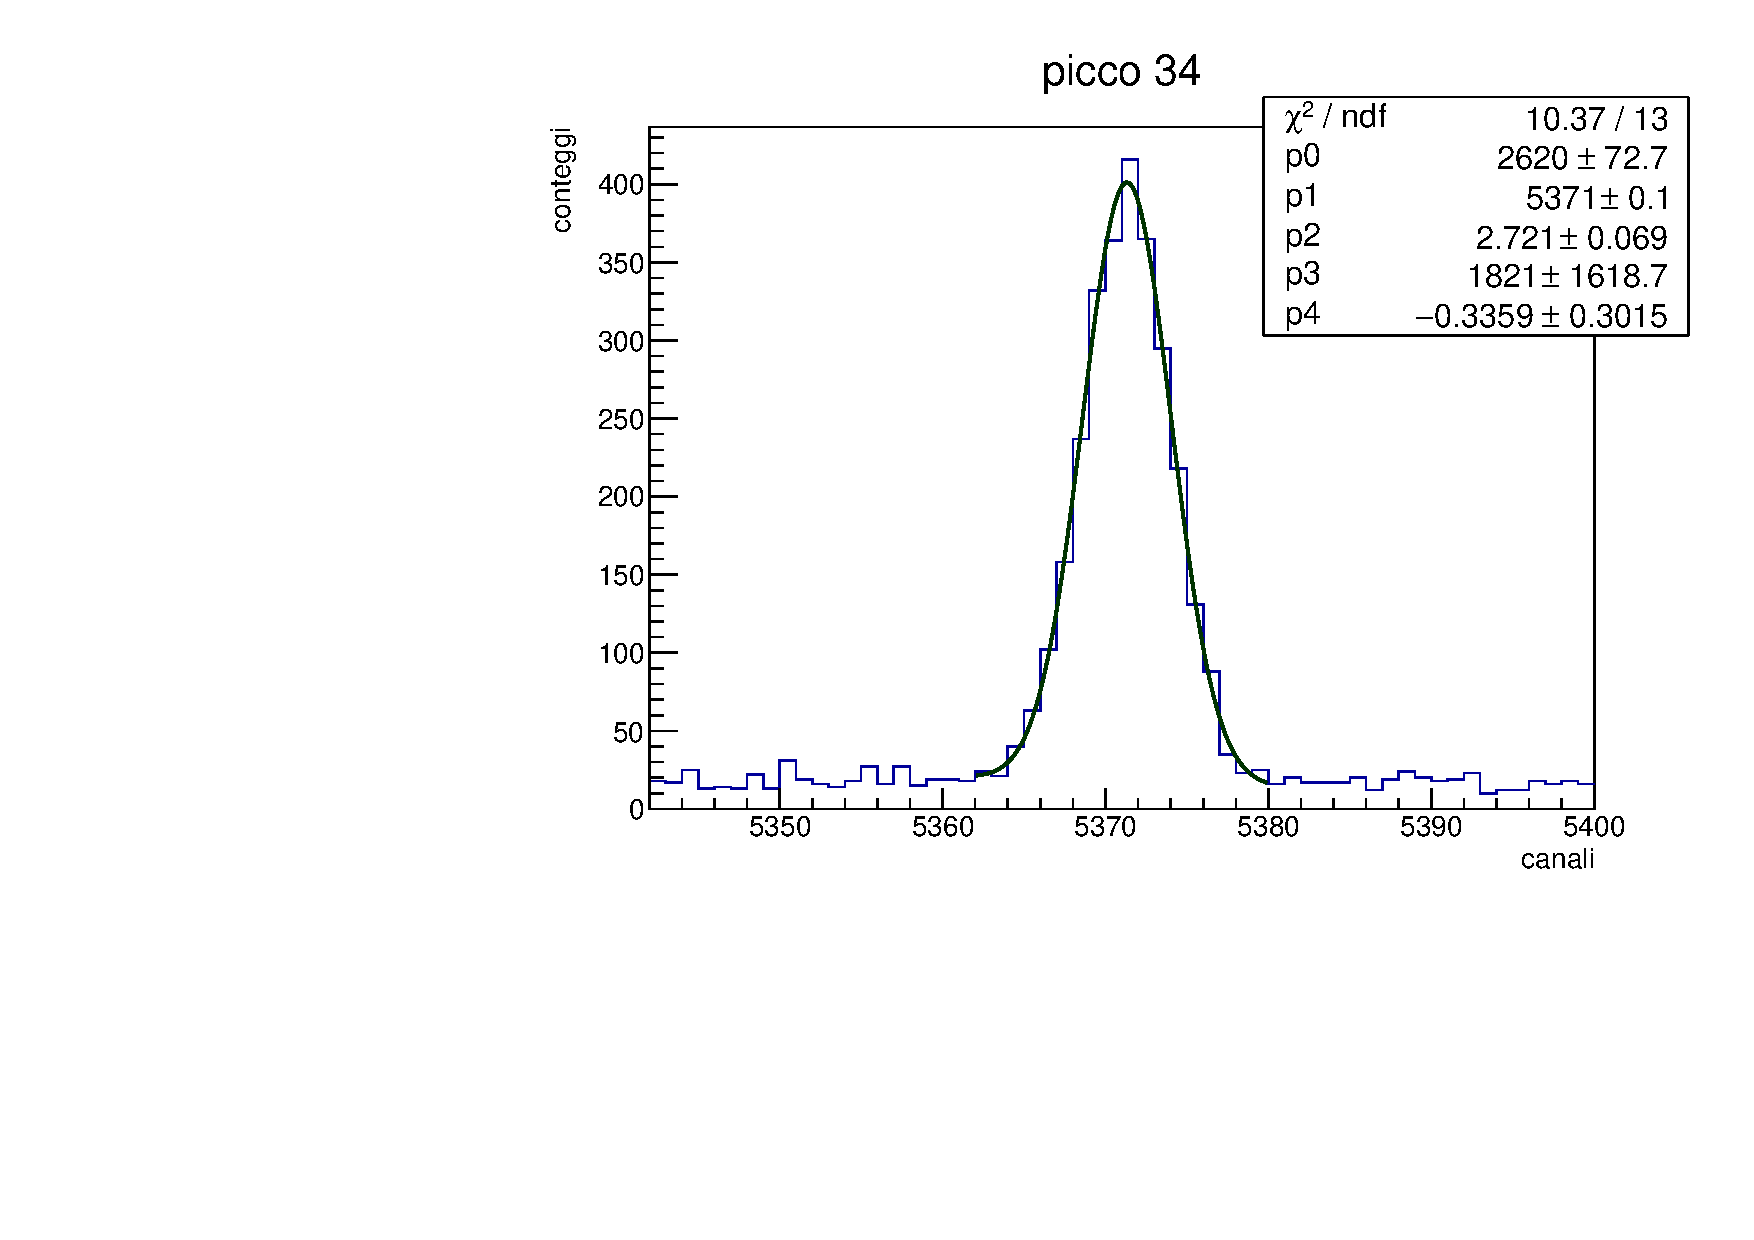
\includegraphics[width=2.2cm]{grafici/picco_incognita_germanio_34.pdf}
                    }
                \subfigure[picco 35]
                    {
                        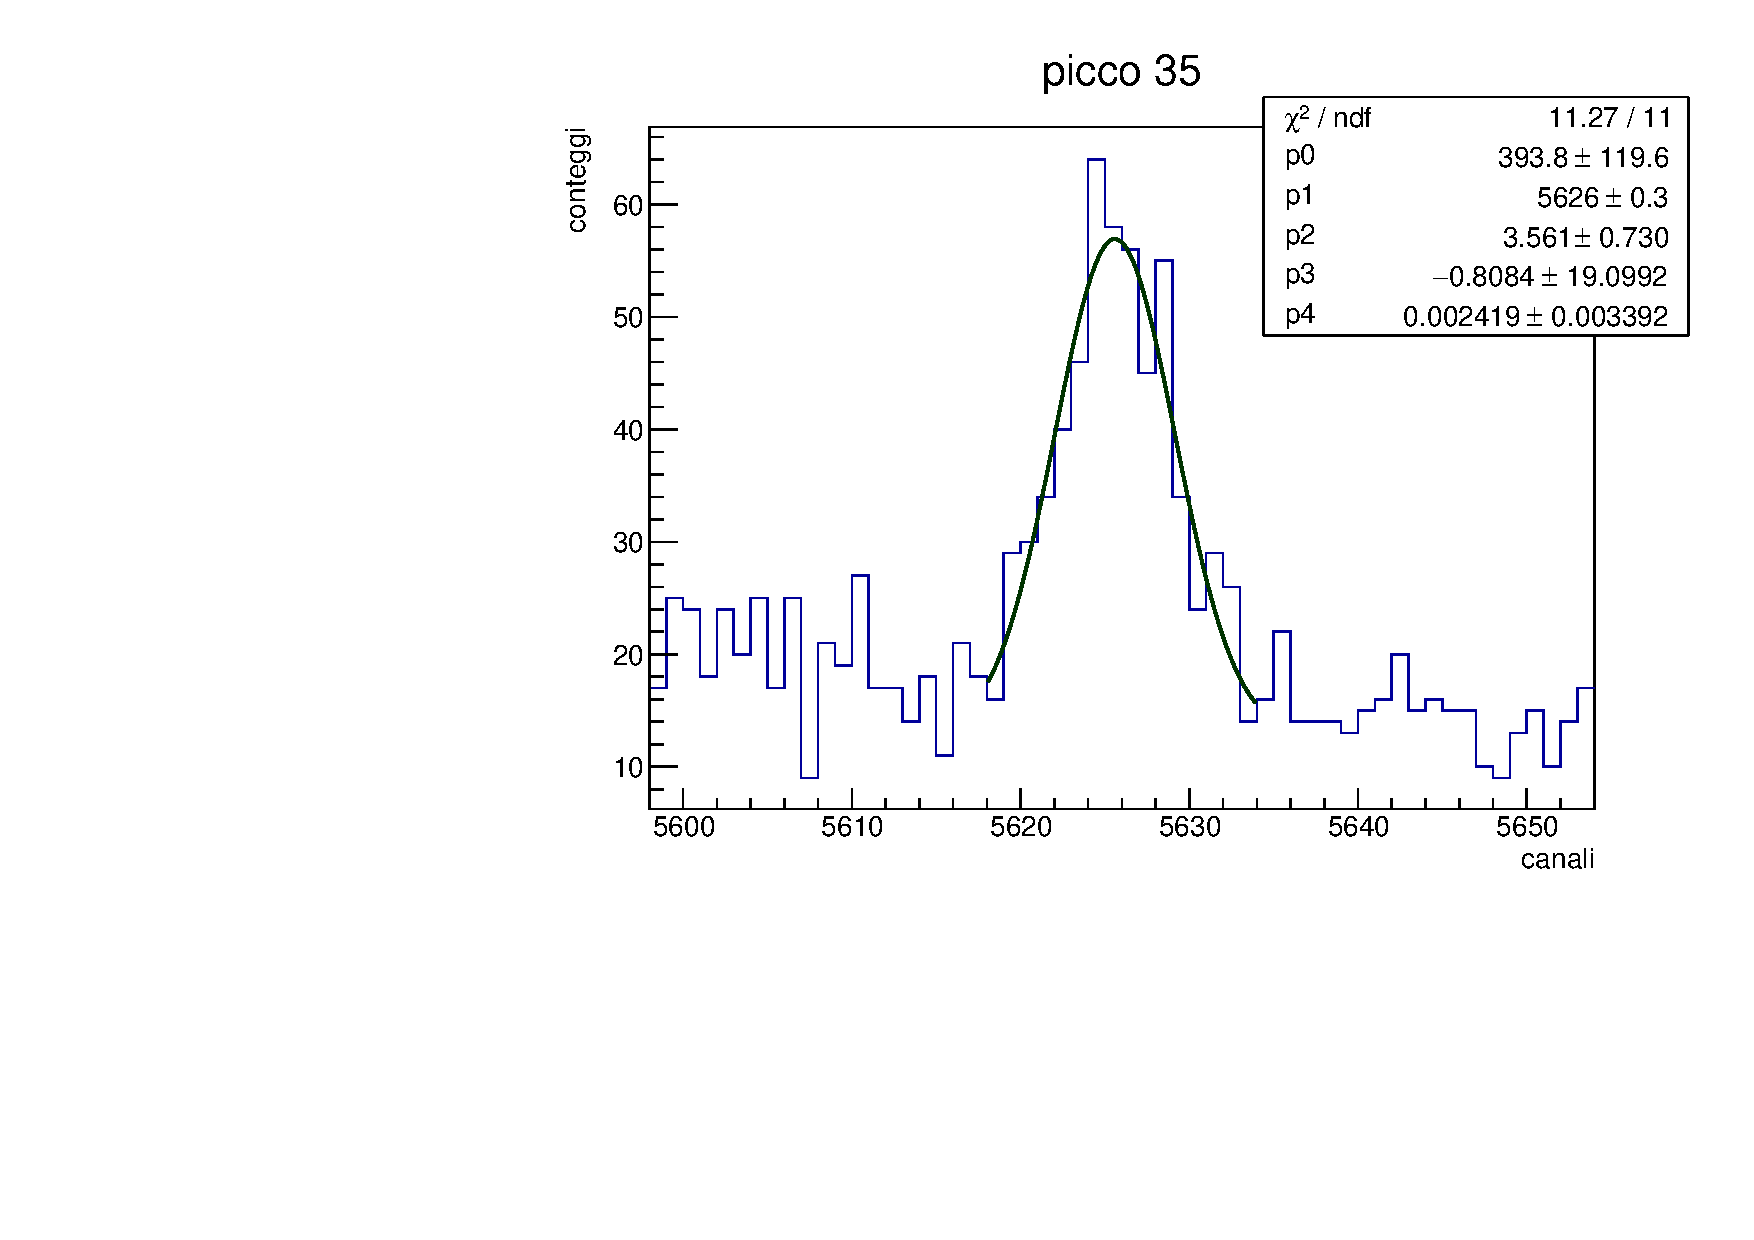
\includegraphics[width=2.2cm]{grafici/picco_incognita_germanio_35.pdf}
                    }

                \subfigure[picco 36]
                    {
                        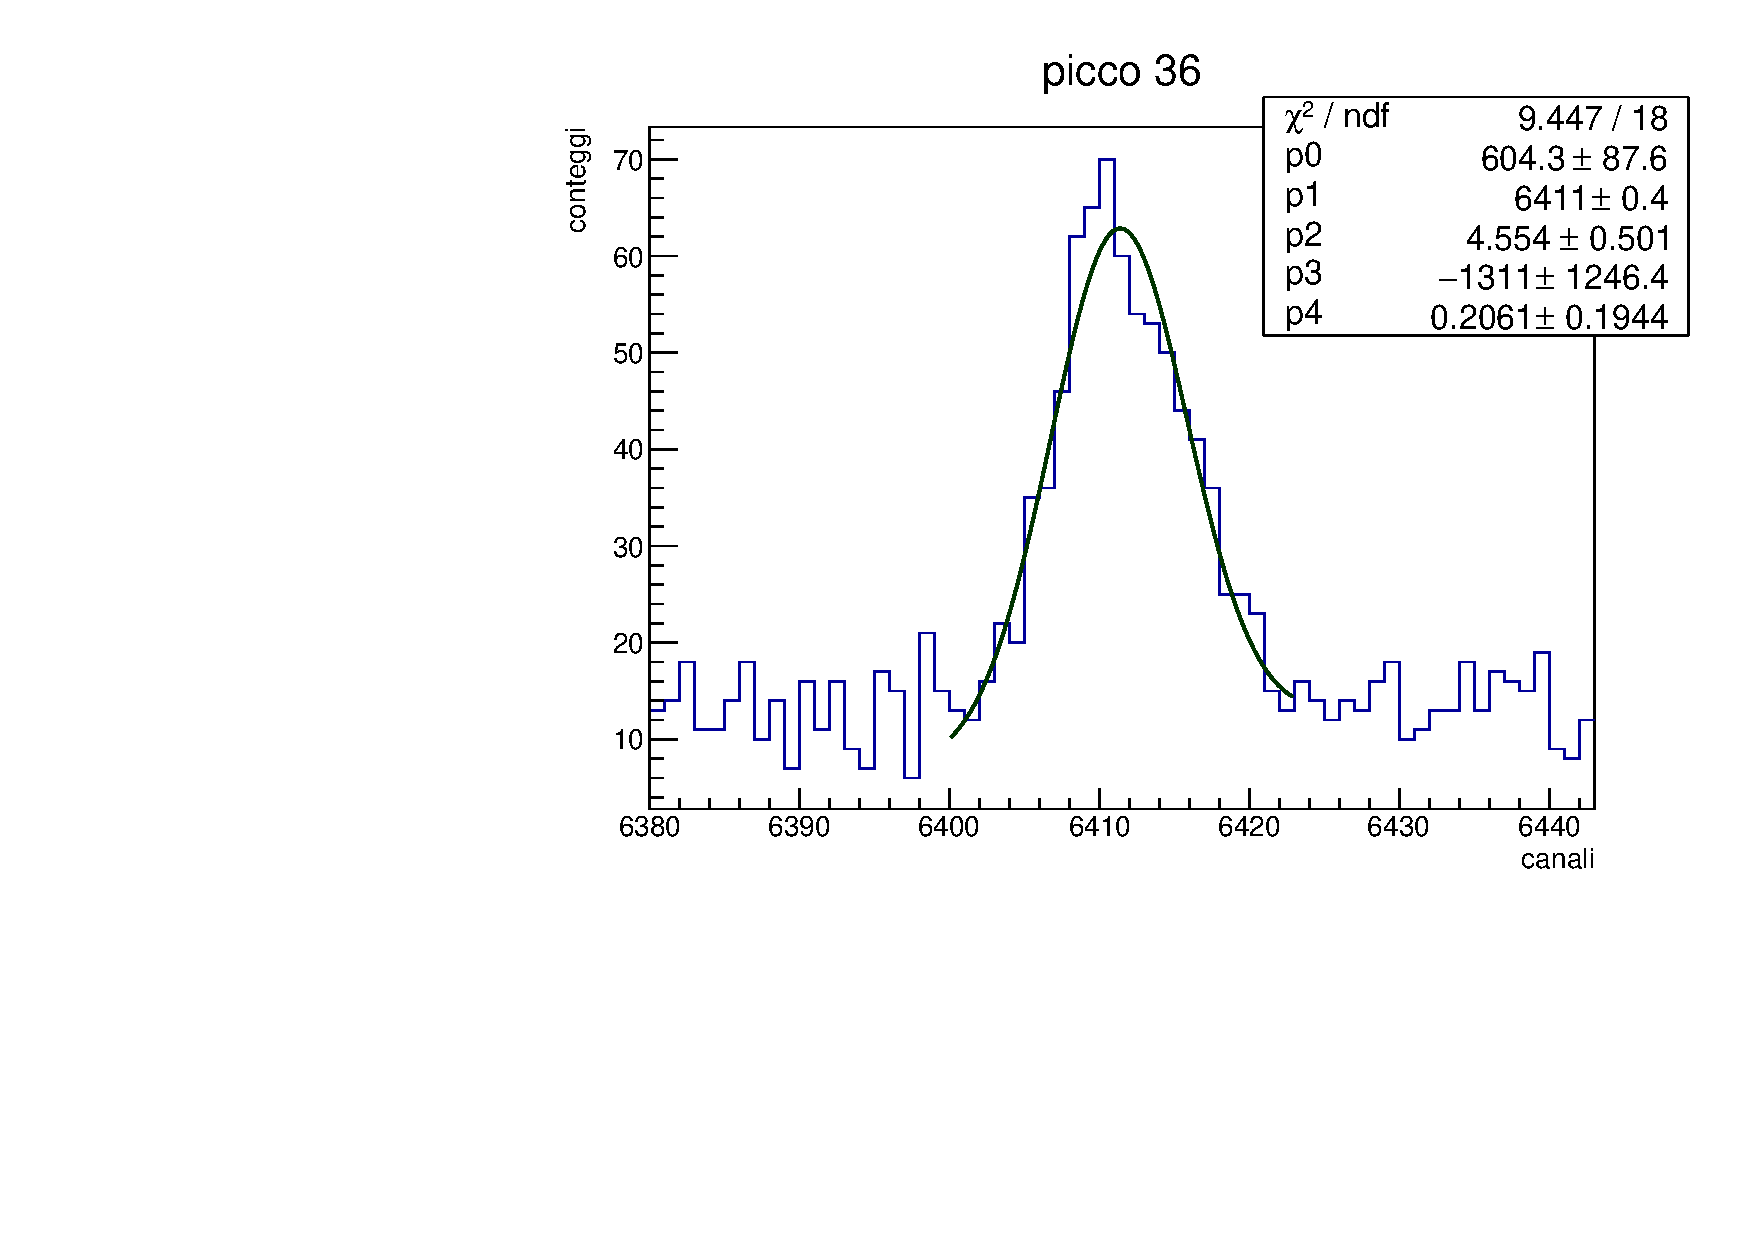
\includegraphics[width=2.2cm]{grafici/picco_incognita_germanio_36.pdf}
                    }
                \subfigure[picco 37]
                    {
                        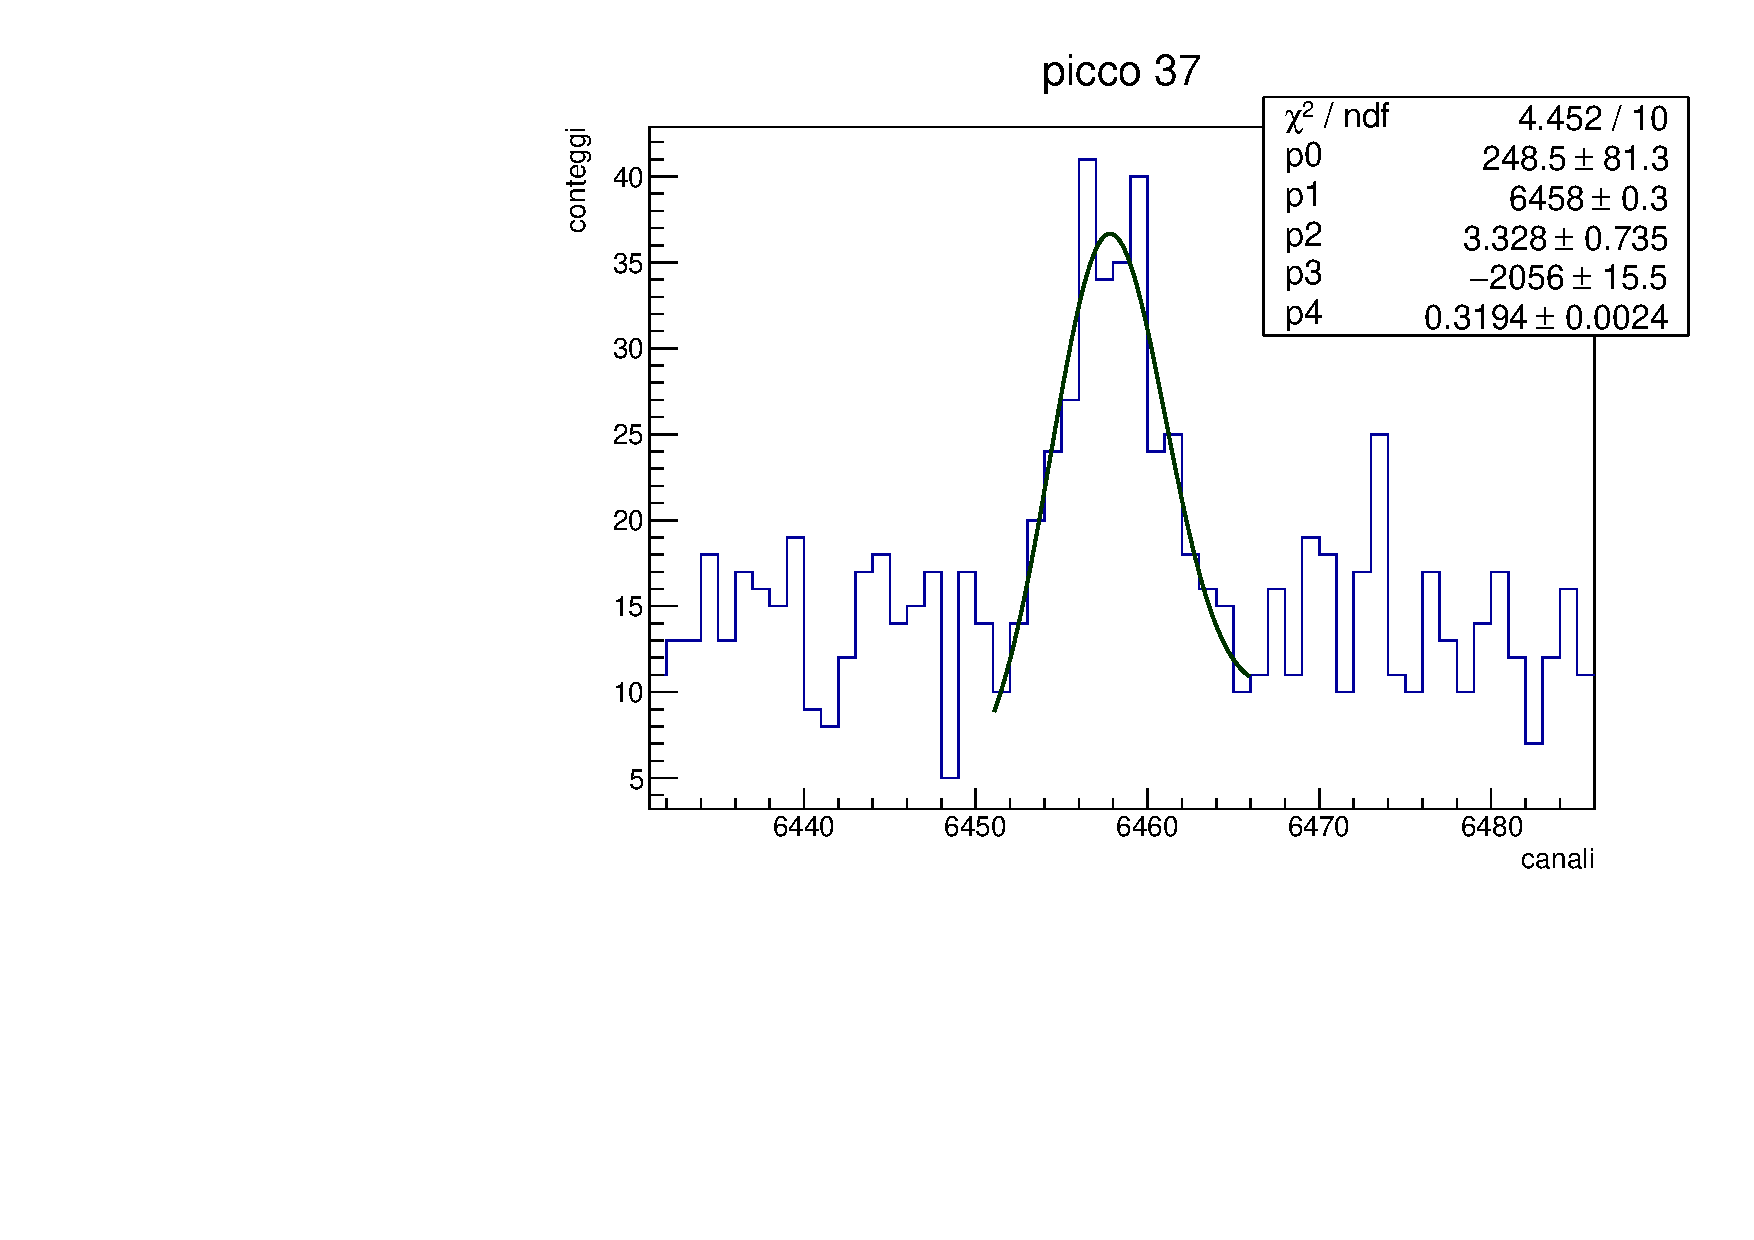
\includegraphics[width=2.2cm]{grafici/picco_incognita_germanio_37.pdf}
                    }
                \subfigure[picco 38]
                    {
                        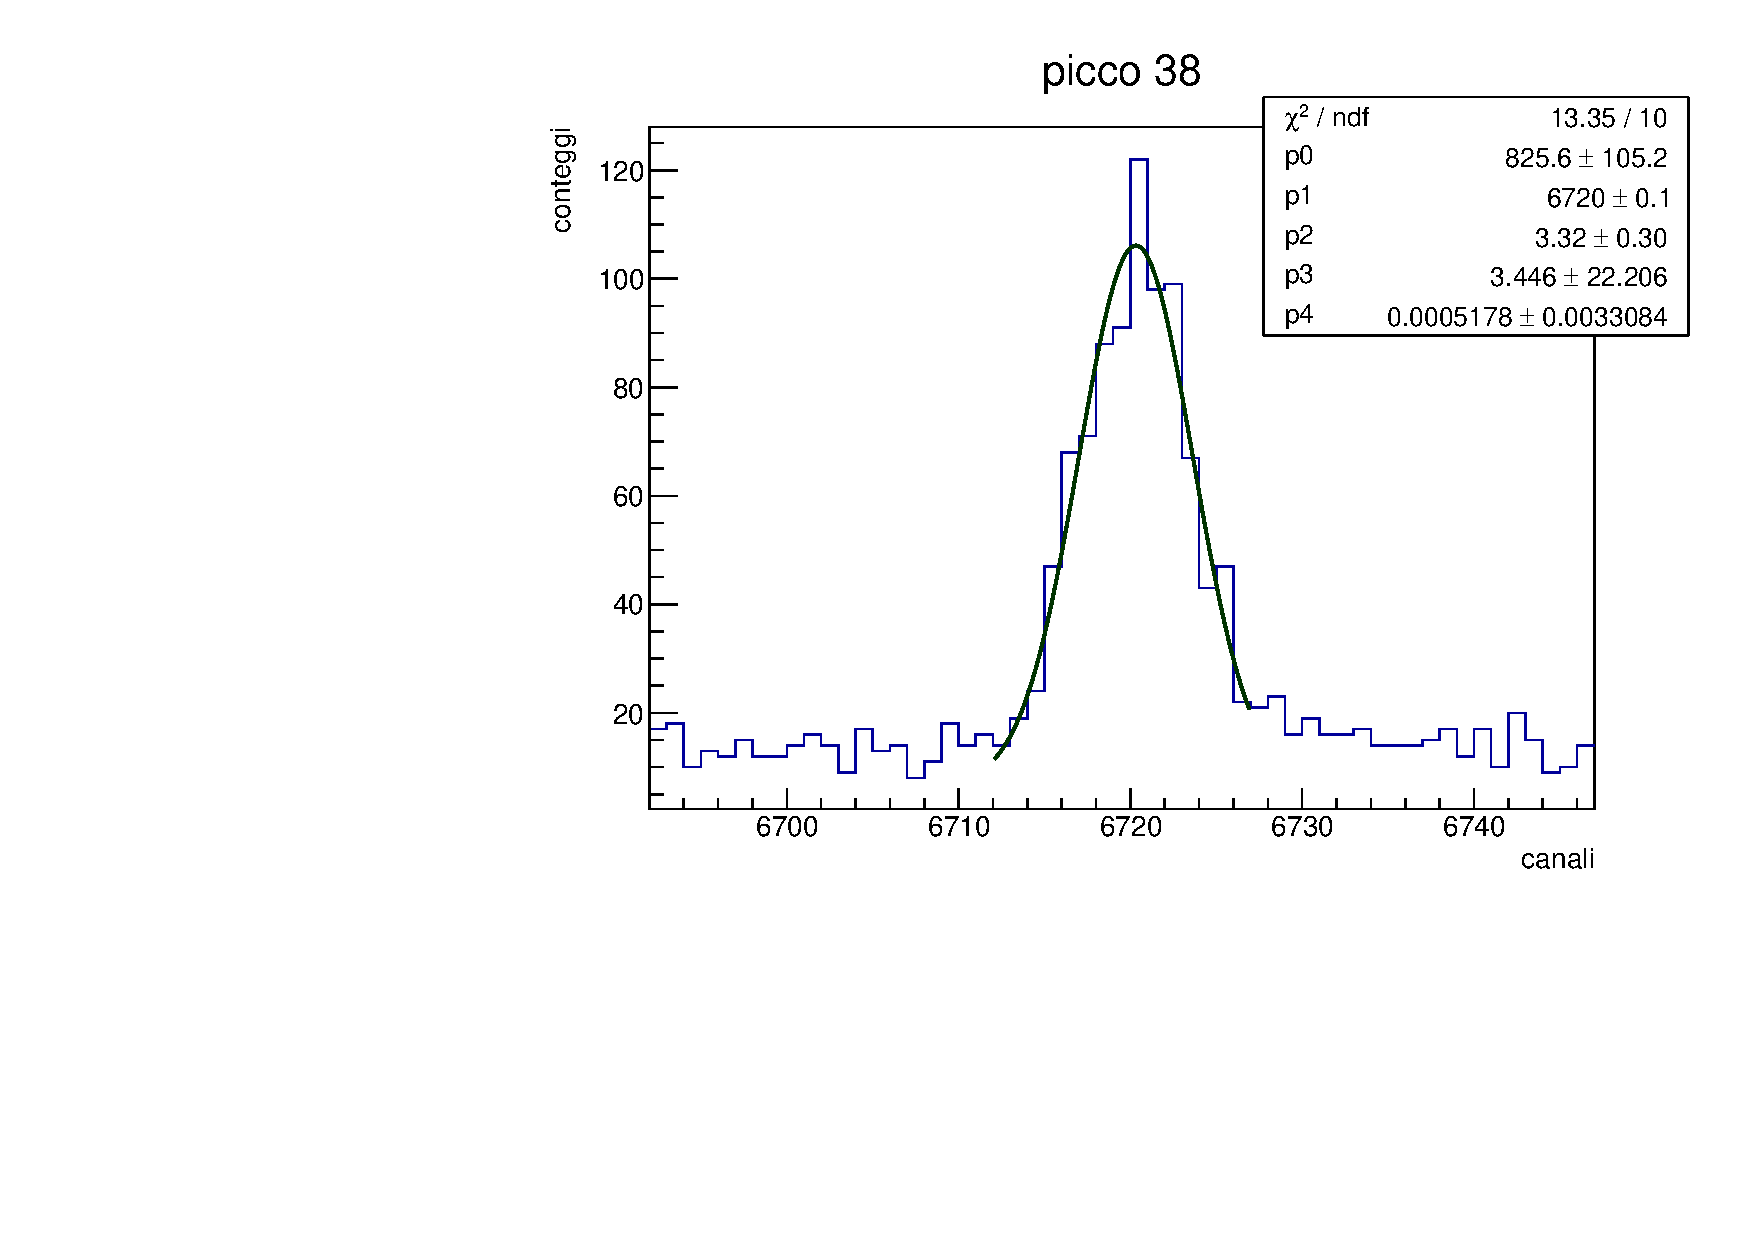
\includegraphics[width=2.2cm]{grafici/picco_incognita_germanio_38.pdf}
                    }
                \subfigure[picco 39]
                    {
                        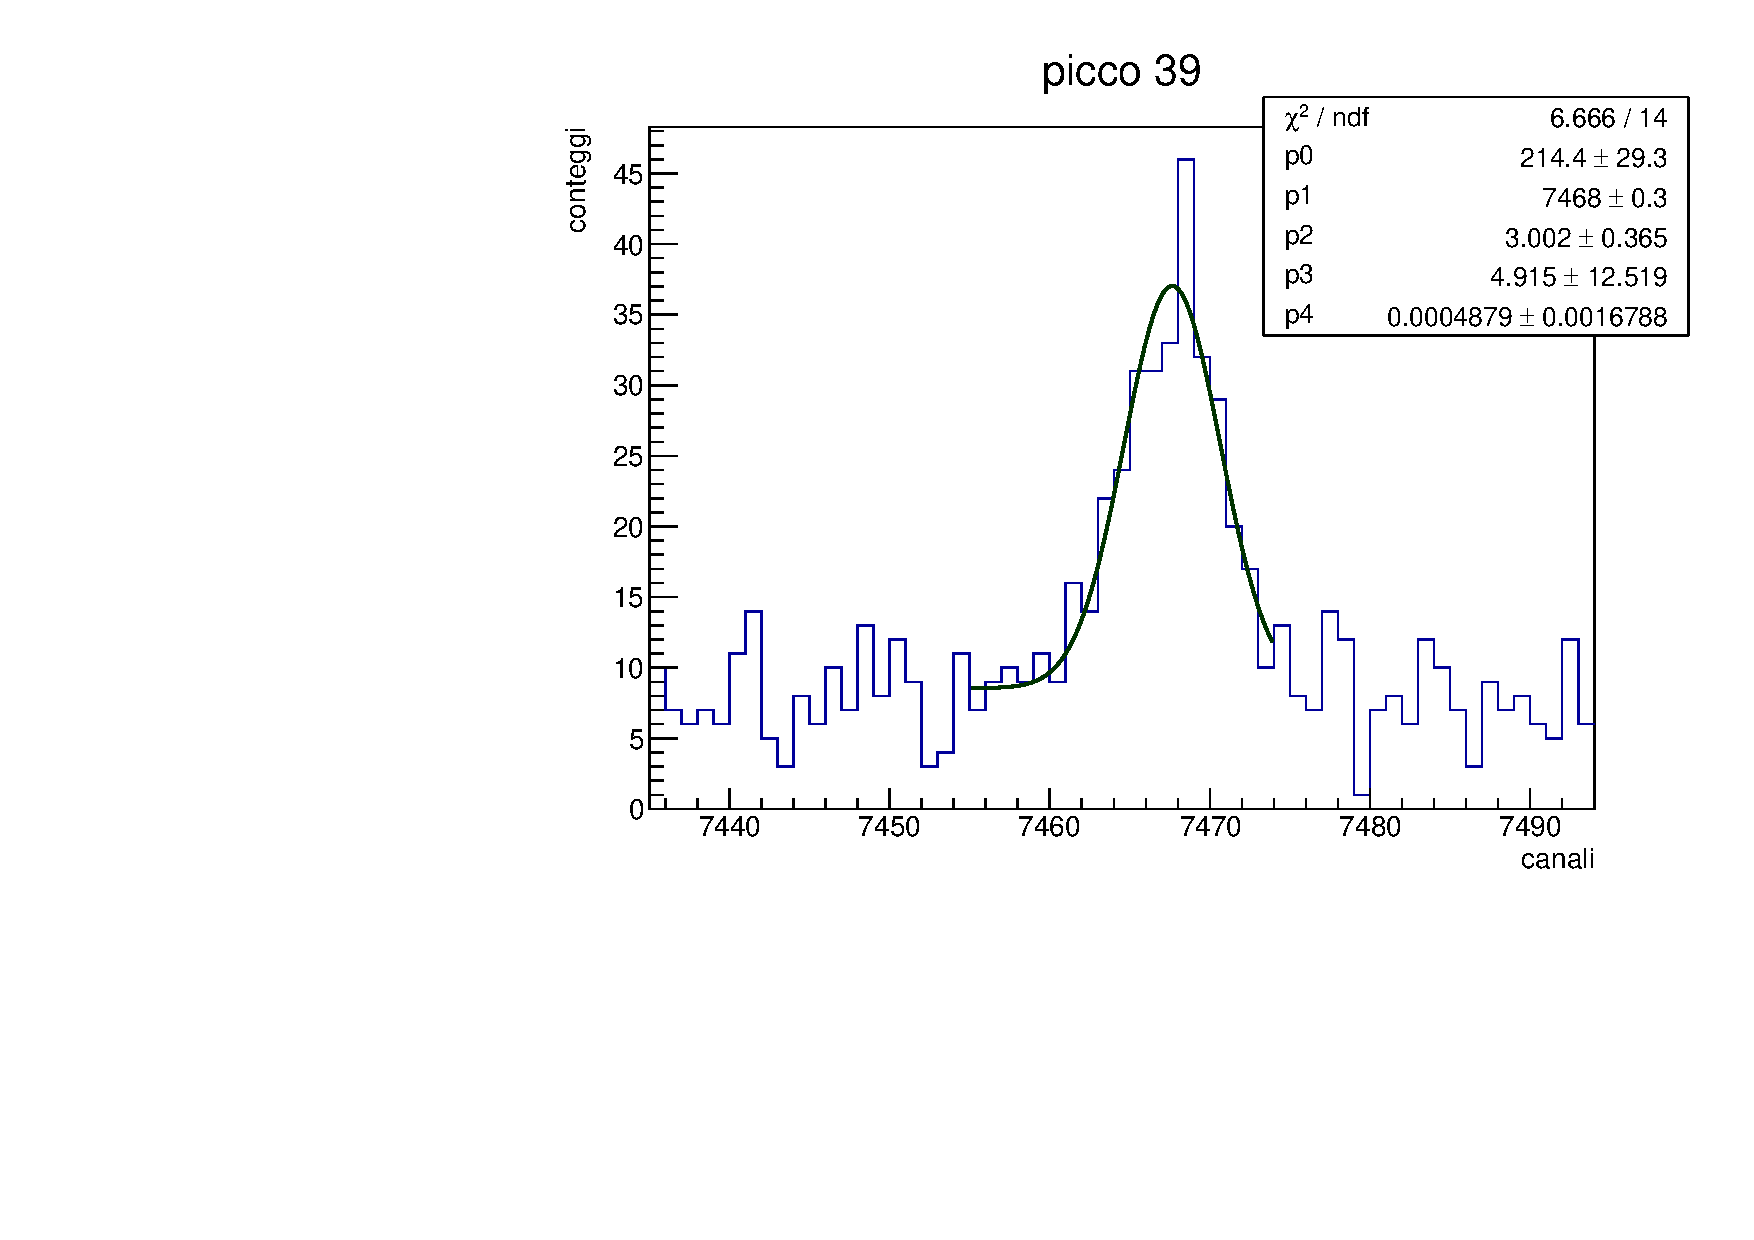
\includegraphics[width=2.2cm]{grafici/picco_incognita_germanio_39.pdf}
                    }
                \subfigure[picco 40]
                    {
                        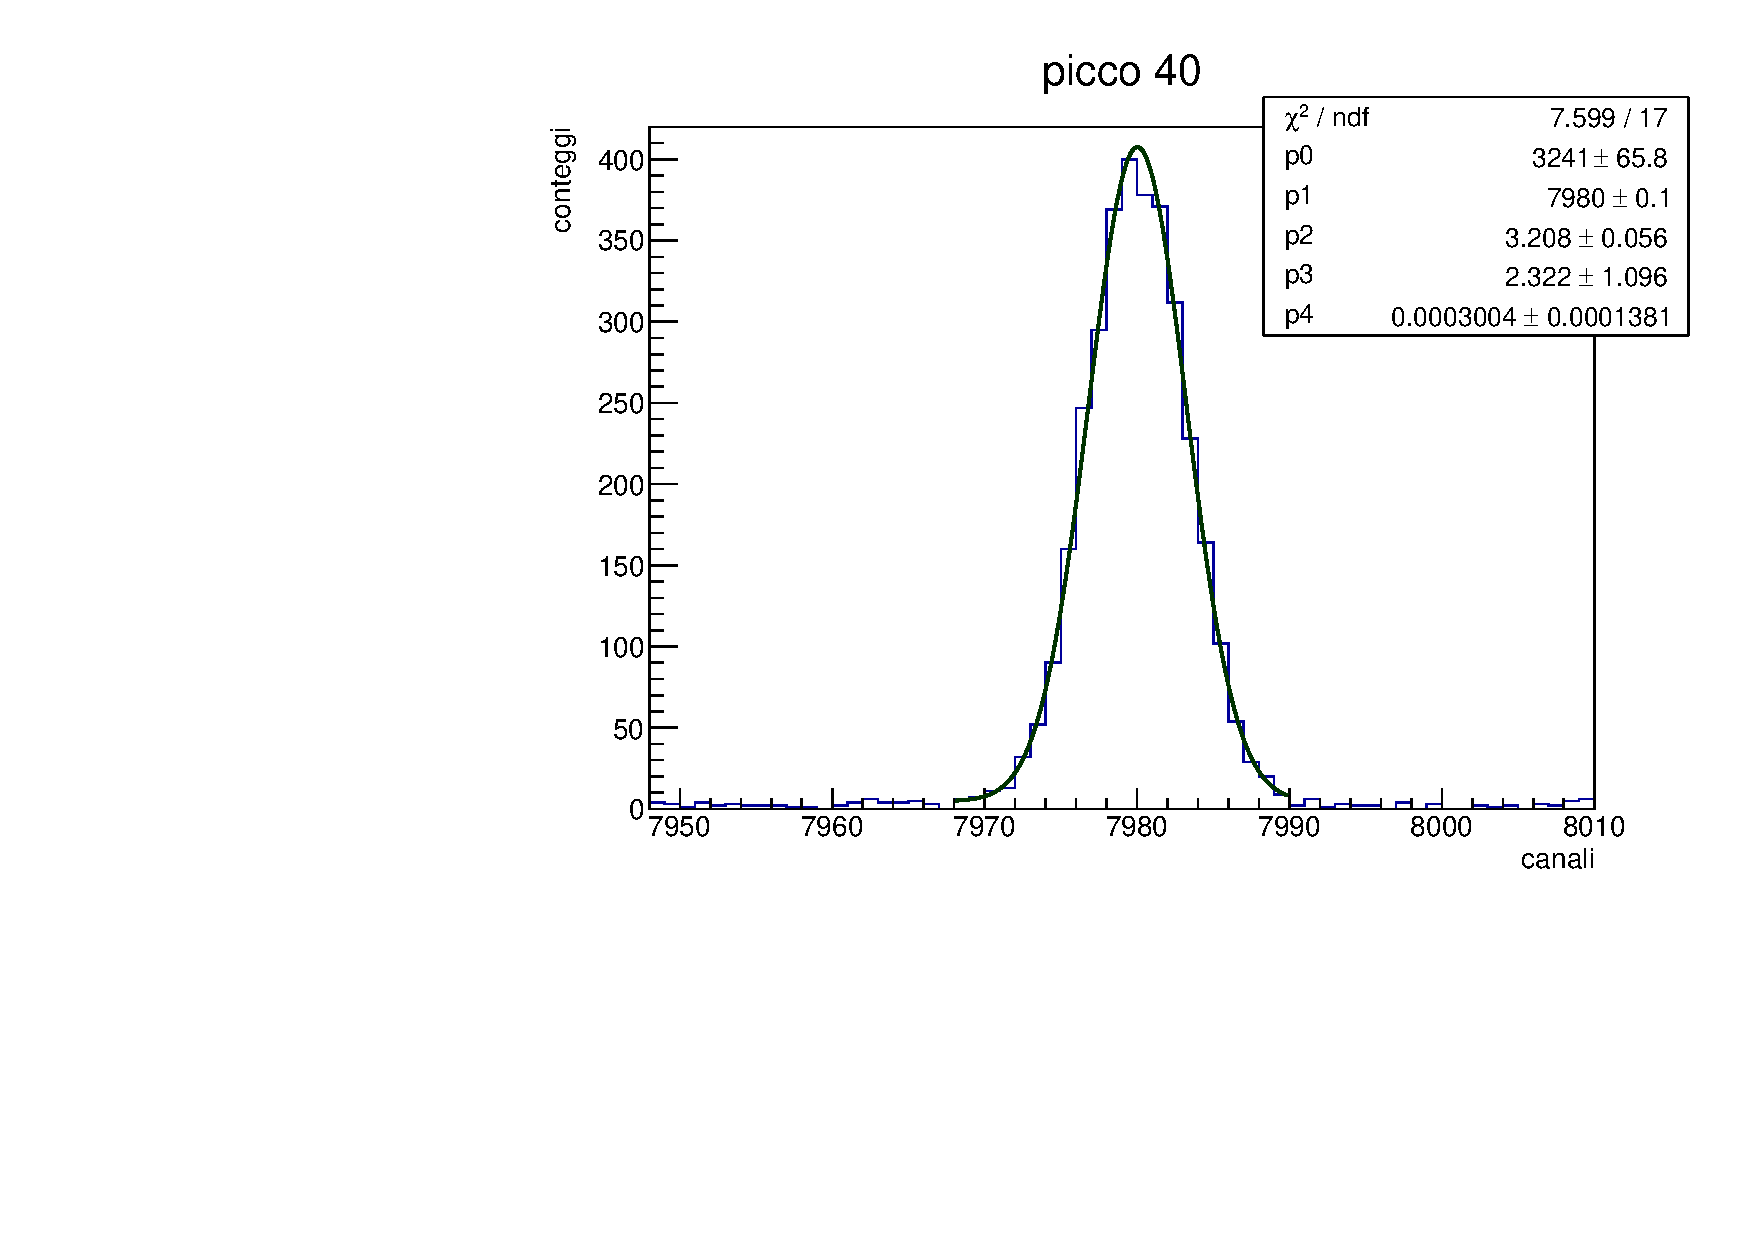
\includegraphics[width=2.2cm]{grafici/picco_incognita_germanio_40.pdf}
                    }
            \end{figure}

            \newpage
            \begin{table}[h!]
                \centering
                \caption{risultati fit sorgente incognita}
                \label{tab:fit_picchi_incognita_germanio}
                    $
                    \begin{array}{ccccccccccc}
	\toprule
	(canali) & N & \delta N & X & \delta X & \sigma & \delta\sigma & FWHM & \delta FWHM & \chi^2 & NDF \\
	\midrule
	\text{picco 1} & 4348 & 1550 &  526.10 & 0.27  &  2.20 & 0.42  &  5.17 & 0.98  & 2.95 & 5 \\
	\text{picco 2} & 11772 & 372 &  687.157 & 0.035  &  1.694 & 0.043  &  3.99 & 0.10  & 2.74 & 6 \\
	\text{picco 3} & 3776 & 749 &  697.38 & 0.15  &  1.90 & 0.24  &  4.48 & 0.56  & 6.67 & 4 \\
	\text{picco 4} & 8542 & 213 &  860.820 & 0.037  &  1.785 & 0.040  &  4.204 & 0.094  & 4.11 & 9 \\
	\text{picco 5} & 2537 & 181 &  993.146 & 0.090  &  1.70 & 0.11  &  4.01 & 0.25  & 6.39 & 8 \\
	\text{picco 6} & 14565 & 234 &  1034.858 & 0.025  &  1.886 & 0.028  &  4.440 & 0.065  & 8.51 & 9 \\
	\text{picco 7} & 2944 & 180 &  1522.32 & 0.11  &  2.76 & 0.16  &  6.50 & 0.37  & 22.09 & 15 \\
	\text{picco 8} & 5450 & 257 &  1744.533 & 0.062  &  2.242 & 0.080  &  5.28 & 0.19  & 5.73 & 8 \\
	\text{picco 9} & 12222 & 162 &  1824.698 & 0.025  &  2.061 & 0.026  &  4.854 & 0.061  & 12.87 & 11 \\
	\text{picco 10} & 1574 & 338 &  2186.75 & 0.24  &  2.81 & 0.37  &  6.62 & 0.87  & 3.85 & 8 \\
	\text{picco 11} & 1101 & 111 &  2313.24 & 0.16  &  2.21 & 0.19  &  5.19 & 0.45  & 7.03 & 11 \\
	\text{picco 12} & 471 & 201 &  2366.18 & 0.32  &  1.80 & 0.48  &  4.23 & 1.14  & 5.16 & 5 \\
	\text{picco 13} & 741 & 162 &  2394.71 & 0.32  &  2.74 & 0.45  &  6.46 & 1.05  & 7.46 & 11 \\
	\text{picco 14} & 787 & 237 &  2596.38 & 0.36  &  2.81 & 0.58  &  6.61 & 1.37  & 9.12 & 9 \\
	\text{picco 15} & 3830 & 221 &  2751.579 & 0.079  &  2.30 & 0.11  &  5.42 & 0.27  & 3.20 & 4 \\
	\text{picco 16} & 823 & 133 &  2821.73 & 0.25  &  2.69 & 0.34  &  6.34 & 0.80  & 6.32 & 11 \\
	\text{picco 17} & 769 & 126 &  2916.18 & 0.16  &  2.18 & 0.29  &  5.13 & 0.68  & 7.11 & 7 \\
	\text{picco 18} & 2182 & 146 &  2928.940 & 0.096  &  2.28 & 0.12  &  5.37 & 0.28  & 7.39 & 8 \\
	\text{picco 19} & 3025 & 98 &  3393.499 & 0.060  &  2.414 & 0.070  &  5.68 & 0.16  & 10.78 & 12 \\
	\text{picco 20} & 1166 & 168 &  3755.11 & 0.18  &  2.58 & 0.26  &  6.06 & 0.60  & 15.82 & 13 \\
	\text{picco 21} & 368 & 105 &  3501.14 & 0.43  &  2.92 & 0.63  &  6.88 & 1.48  & 15.12 & 11 \\
	\text{picco 22} & 654 & 63 &  4183.49 & 0.15  &  2.17 & 0.19  &  5.12 & 0.46  & 6.75 & 10 \\
	\text{picco 23} & 528 & 400 &  4256.97 & 0.43  &  4.21 & 1.53  &  9.91 & 3.61  & 7.09 & 7 \\
	\text{picco 24} & 513 & 189 &  4276.87 & 0.20  &  2.62 & 0.59  &  6.18 & 1.39  & 5.31 & 6 \\
	\text{picco 25} & 15321 & 135 &  4438.909 & 0.024  &  2.648 & 0.020  &  6.235 & 0.047  & 19.05 & 18 \\
	\text{picco 26} & 148 & 77 &  4547.33 & 0.30  &  1.78 & 0.64  &  4.20 & 1.51  & 0.94 & 4 \\
	\text{picco 27} & 686 & 241 &  4587.38 & 0.22  &  3.64 & 0.72  &  8.56 & 1.69  & 4.24 & 8 \\
	\text{picco 28} & 675 & 148 &  4829.91 & 0.19  &  3.42 & 0.47  &  8.06 & 1.11  & 11.43 & 8 \\
	\text{picco 29} & 797 & 95 &  4843.76 & 0.18  &  2.63 & 0.23  &  6.18 & 0.55  & 19.81 & 10 \\
	\text{picco 30} & 296 & 131 &  4929.81 & 0.65  &  3.74 & 1.09  &  8.80 & 2.58  & 7.39 & 12 \\
	\text{picco 31} & 429 & 169 &  4960.52 & 0.31  &  4.05 & 0.90  &  9.54 & 2.13  & 10.35 & 9 \\
	\text{picco 32} & 437 & 209 &  5052.49 & 0.29  &  3.99 & 0.96  &  9.39 & 2.27  & 9.80 & 8 \\
	\text{picco 33} & 493 & 60 &  5264.23 & 0.23  &  2.87 & 0.30  &  6.77 & 0.70  & 5.79 & 12 \\
	\text{picco 34} & 2620 & 73 &  5371.320 & 0.069  &  2.721 & 0.069  &  6.41 & 0.16  & 10.37 & 13 \\
	\text{picco 35} & 394 & 120 &  5625.59 & 0.27  &  3.56 & 0.73  &  8.39 & 1.72  & 11.27 & 11 \\
	\text{picco 36} & 604 & 88 &  6411.31 & 0.37  &  4.55 & 0.50  &  10.72 & 1.18  & 9.45 & 18 \\
	\text{picco 37} & 249 & 81 &  6457.70 & 0.31  &  3.33 & 0.74  &  7.84 & 1.73  & 4.45 & 10 \\
	\text{picco 38} & 826 & 105 &  6720.32 & 0.15  &  3.32 & 0.30  &  7.82 & 0.71  & 13.35 & 10 \\
	\text{picco 39} & 214 & 29 &  7467.65 & 0.31  &  3.00 & 0.36  &  7.07 & 0.86  & 6.67 & 14 \\
	\text{picco 40} & 3241 & 66 &  7980.028 & 0.060  &  3.208 & 0.056  &  7.55 & 0.13  & 7.60 & 17 \\
	\bottomrule
\end{array}%
                    $
            \end{table}

            La tabella \ref{tab:energie_calcolate_incognita} mostra le energie calcolate per la sorgente incognita sfruttando i parametri di calibrazione per la conversione.
            \begin{table}[h!]
                \centering
                \caption{energie sorgente incognita}
                \label{tab:energie_calcolate_incognita}
                $
                \begin{array}{ccccc}
	\toprule
	(keV) & E & \delta E & FWHM & \delta FWHM \\
	\midrule
	\text{picco 1} &  185.456 & 0.088  &  1.68 & 0.32  \\ 
	\text{picco 2} &  237.777 & 0.012  &  1.296 & 0.032  \\ 
	\text{picco 3} &  241.098 & 0.049  &  1.46 & 0.18  \\ 
	\text{picco 4} &  294.193 & 0.013  &  1.366 & 0.031  \\ 
	\text{picco 5} &  337.181 & 0.030  &  1.303 & 0.081  \\ 
	\text{picco 6} &  350.7315 & 0.0094  &  1.442 & 0.021  \\ 
	\text{picco 7} &  509.089 & 0.036  &  2.11 & 0.12  \\ 
	\text{picco 8} &  581.277 & 0.021  &  1.715 & 0.062  \\ 
	\text{picco 9} &  607.319 & 0.010  &  1.577 & 0.020  \\ 
	\text{picco 10} &  724.936 & 0.078  &  2.15 & 0.28  \\ 
	\text{picco 11} &  766.028 & 0.052  &  1.69 & 0.15  \\ 
	\text{picco 12} &  783.23 & 0.10  &  1.37 & 0.37  \\ 
	\text{picco 13} &  792.49 & 0.10  &  2.10 & 0.34  \\ 
	\text{picco 14} &  858.01 & 0.12  &  2.15 & 0.45  \\ 
	\text{picco 15} &  908.427 & 0.027  &  1.761 & 0.088  \\ 
	\text{picco 16} &  931.216 & 0.082  &  2.06 & 0.26  \\ 
	\text{picco 17} &  961.899 & 0.053  &  1.67 & 0.22  \\ 
	\text{picco 18} &  966.044 & 0.032  &  1.745 & 0.091  \\ 
	\text{picco 19} &  1116.961 & 0.022  &  1.845 & 0.052  \\ 
	\text{picco 20} &  1234.434 & 0.059  &  1.97 & 0.19  \\ 
	\text{picco 21} &  1151.93 & 0.14  &  2.24 & 0.48  \\ 
	\text{picco 22} &  1373.598 & 0.050  &  1.66 & 0.15  \\ 
	\text{picco 23} &  1397.47 & 0.14  &  3.22 & 1.17  \\ 
	\text{picco 24} &  1403.934 & 0.066  &  2.01 & 0.45  \\ 
	\text{picco 25} &  1456.574 & 0.015  &  2.026 & 0.015  \\ 
	\text{picco 26} &  1491.796 & 0.098  &  1.36 & 0.49  \\ 
	\text{picco 27} &  1504.806 & 0.073  &  2.78 & 0.55  \\ 
	\text{picco 28} &  1583.595 & 0.063  &  2.62 & 0.36  \\ 
	\text{picco 29} &  1588.094 & 0.060  &  2.01 & 0.18  \\ 
	\text{picco 30} &  1616.05 & 0.21  &  2.86 & 0.84  \\ 
	\text{picco 31} &  1626.02 & 0.10  &  3.10 & 0.69  \\ 
	\text{picco 32} &  1655.902 & 0.095  &  3.05 & 0.74  \\ 
	\text{picco 33} &  1724.688 & 0.076  &  2.20 & 0.23  \\ 
	\text{picco 34} &  1759.478 & 0.027  &  2.082 & 0.052  \\ 
	\text{picco 35} &  1842.080 & 0.089  &  2.73 & 0.56  \\ 
	\text{picco 36} &  2097.33 & 0.12  &  3.48 & 0.38  \\ 
	\text{picco 37} &  2112.40 & 0.10  &  2.55 & 0.56  \\ 
	\text{picco 38} &  2197.715 & 0.052  &  2.54 & 0.23  \\ 
	\text{picco 39} &  2440.49 & 0.10  &  2.30 & 0.28  \\ 
	\text{picco 40} &  2606.944 & 0.029  &  2.453 & 0.042  \\ 
	\bottomrule
\end{array}
                $
            \end{table}

            \newpage
            Infine, è doverosa una precisazione metodologica: nonostante la sottrazione del fondo sia stata utile in fase di ricerca preliminare dei picchi che dipendessero dalla sorgente e non dal fondo ambientale, i fit numerici sono stati eseguiti sullo spettro grezzo. Questa scelta è stata dettata dal fatto che il tempo di acquisizione della sorgente incognita è stato ben superiore rispetto a quello per il fondo, e dalla formula \eqref{for:sottrazione_fondo} si evince che ciò avrebbe portato a una troppo grande incertezza sperimentale che avrebbe annientato i risultati in termini di significato statistico.

    \section{La coincidenza}
        Il cuore dell'esperimento, ovvero l'emissione in coincidenza dei due fotoni dal cobalto-60, non richiede lo sviluppo di nuovi codici: basta utilizzare la macro \textit{spettro.cpp} per visualizzare lo spettro di un picco nel rivelatore al germanio e l'altro in quello al fluoruro di bario, avendo semplicemente cura di selezionare i file di input corretti e di utilizzare il fit con una doppia gaussiana qualora la scarsa risoluzione lo richiedesse.

        \subsection*{I risultati ottenuti}
            La figura \ref{fig:picchi_cobalto_coincidenza} mostra i fit degli spettri con entrambi i picchi e con uno solo per i due rivelatori, solamente nel range di interesse.
            
            \begin{figure}[h!]
                \centering
                \caption{spettri in canali cobalto-60}
                \label{fig:picchi_cobalto_coincidenza}
                \subfigure[picchi BaF (doppia gaussiana)]
                    {
                        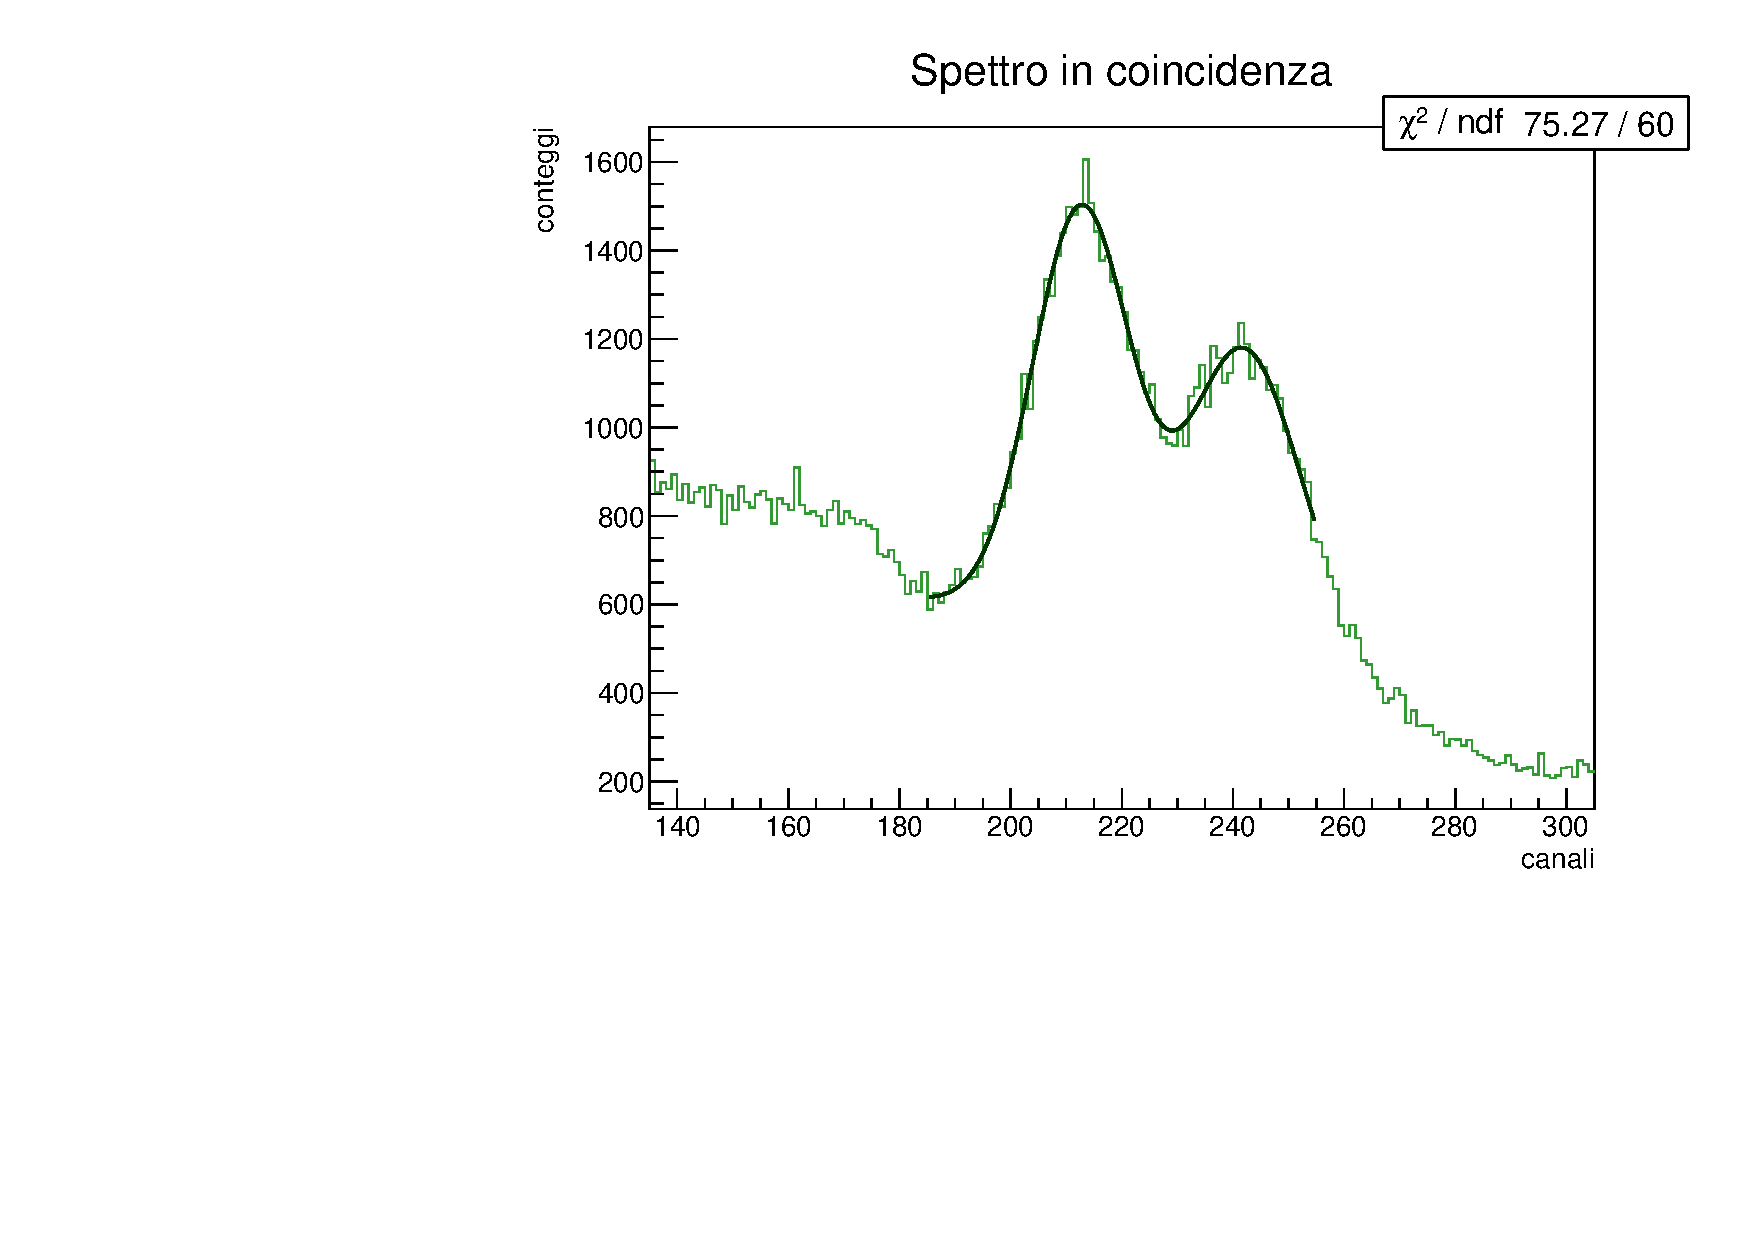
\includegraphics[width=4.5cm]{grafici/spettro_cobalto_baf.pdf}
                    }
                \subfigure[picco bassa energia BaF (soglia)]
                    {
                        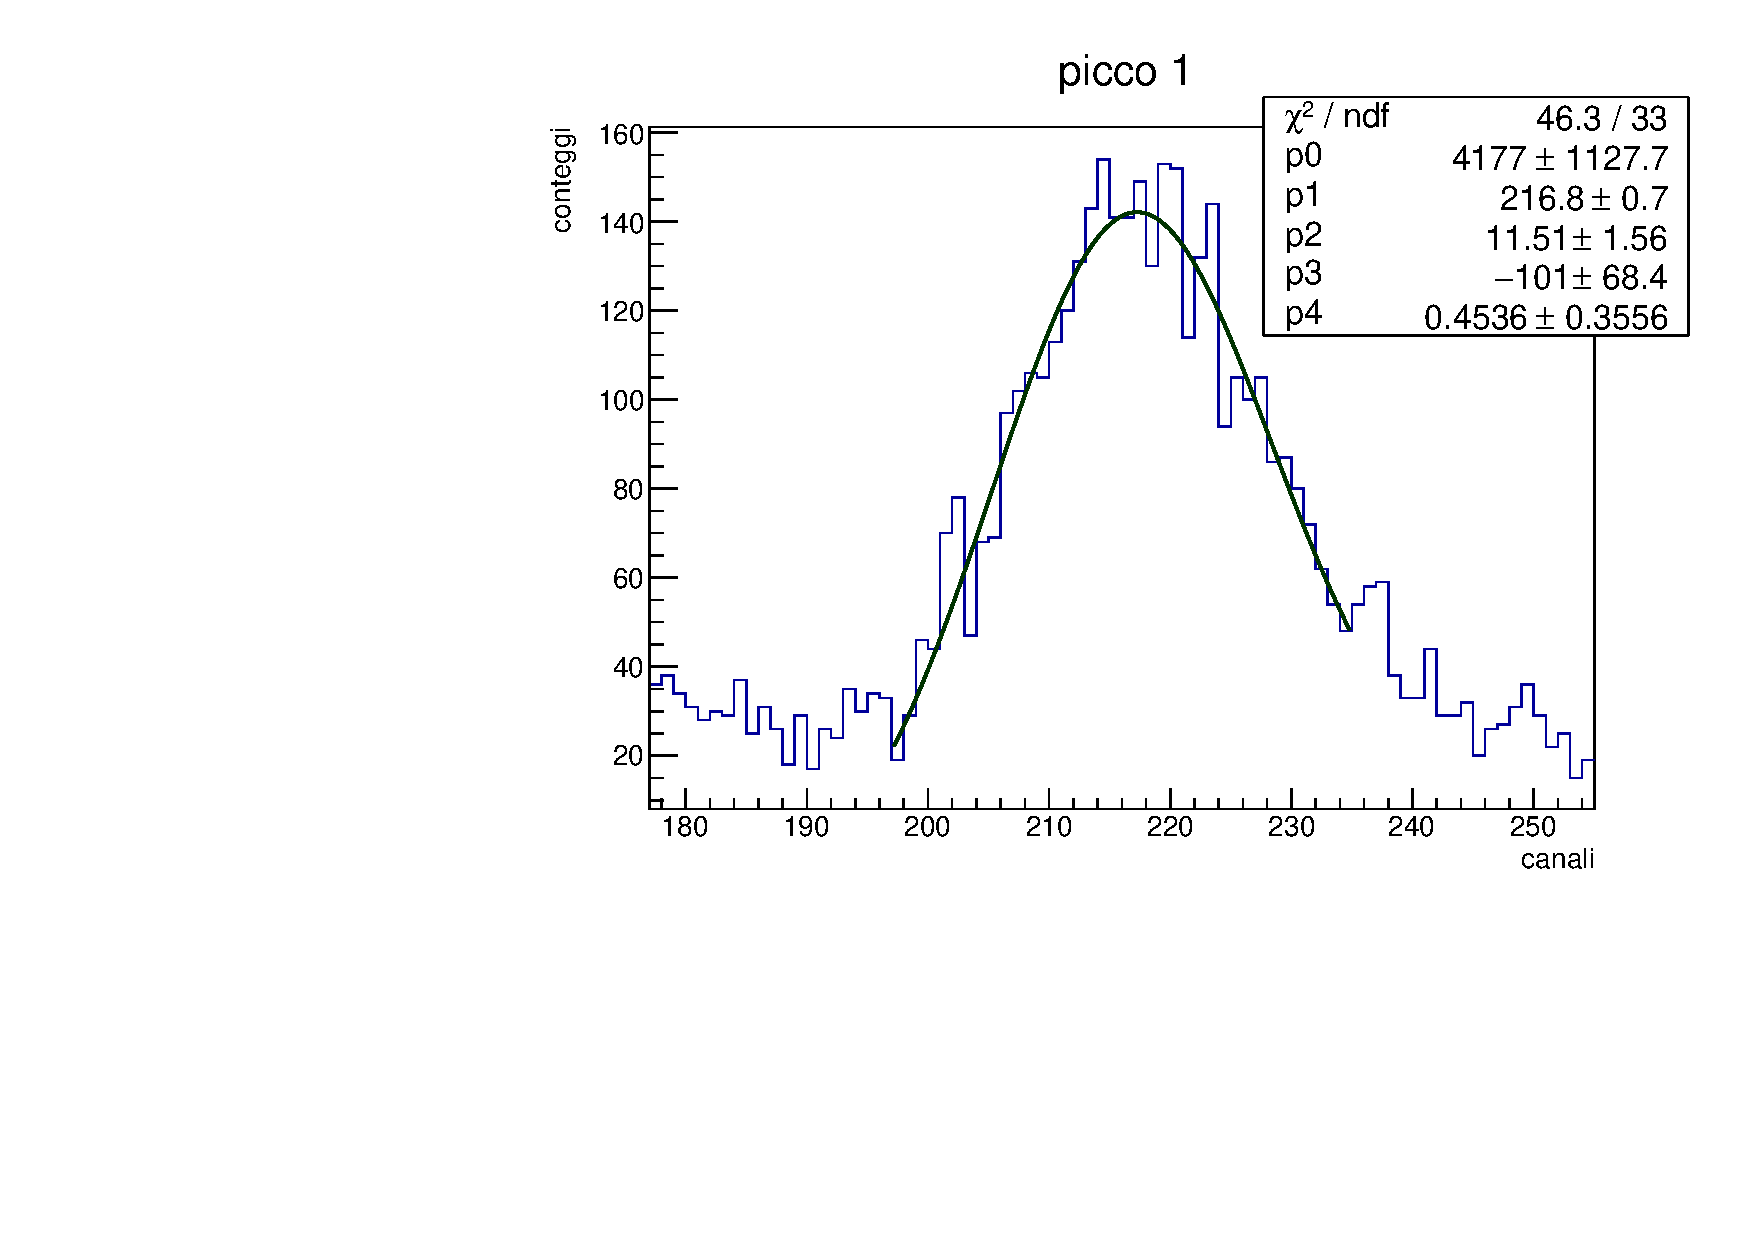
\includegraphics[width=4.5cm]{grafici/picco_cobalto_baf_monopicco_1.pdf}
                    } 
                \subfigure[picco alta energia HpGe (soglia)]
                    {
                        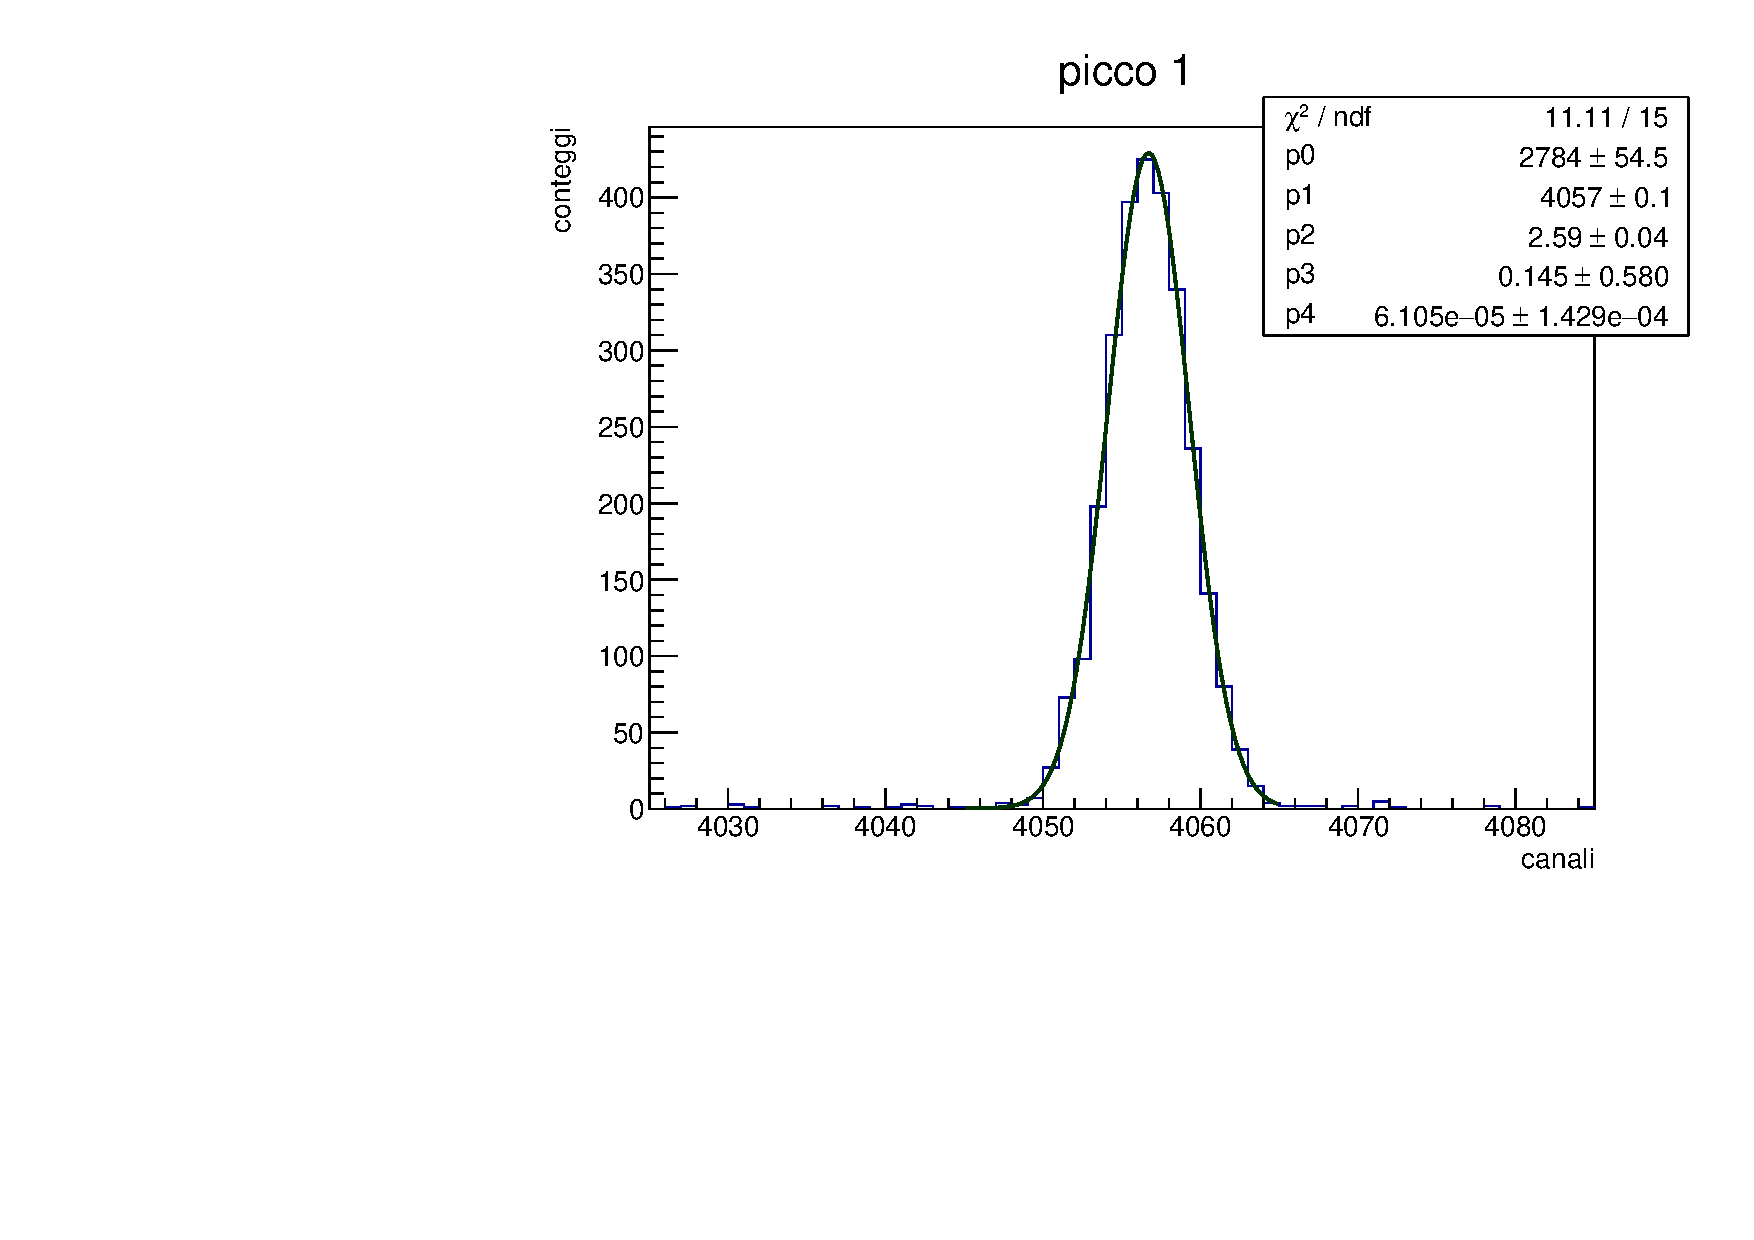
\includegraphics[width=4.5cm]{grafici/picco_cobalto_germanio_monopicco_1.pdf}
                    } 
            \end{figure}

            La tabella \ref{tab:fit_coincidenza} mostra i risultati numerici dei fit gaussiani precedenti.
            \begin{table}[h!]
                \centering
                \caption{risultati fit coincidenza}
                \label{tab:fit_coincidenza}
                \subtable[cobalto-60 nel BaF]
                    {
                        $
                        \begin{array}{ccccccccc}
	\toprule
	(canali) & N & \delta N & X & \delta X & \sigma & \delta\sigma & FWHM & \delta FWHM  \\
	\midrule
	\text{picco 1} & 20625 & 633 &  212.77 & 0.18  &  8.83 & 0.21  &  20.79 & 0.49  \\
	\text{picco 1} & 16702 & 770 &  242.01 & 0.27  &  10.03 & 0.35  &  23.62 & 0.83  \\
	\bottomrule
\end{array}%
                        $
                    }
                \subtable[cobalto-60 nel BaF (con soglia)]
                    {
                        $
                        \begin{array}{ccccccccccc}
	\toprule
	(canali) & N & X & \sigma & FWHM & \delta N & \delta X & \delta\sigma & \delta FWHM & \chi^2 & NDF \\
	\midrule
	\text{picco 1} & 4177 & 216.842 & 11.513 & 27.111 & 1128 & 0.707 & 1.558 & 3.669 & 46.30 & 33 \\
	\bottomrule
\end{array}%
                        $
                    }
                \subtable[cobalto-60 nell'HpGe (con soglia)]
                    {
                        $
                        \begin{array}{ccccccccccc}
	\toprule
	(canali) & N & X & \sigma & FWHM & \delta N & \delta X & \delta\sigma & \delta FWHM & \chi^2 & NDF \\
	\midrule
	\text{picco 2} & 2784 & 4056.700 & 2.590 & 6.099 & 55 & 0.050 & 0.041 & 0.097 & 11.11 & 15 \\
	\bottomrule
\end{array}%
                        $
                    }
            \end{table}

            Infine, ha significato indicare la risoluzione percentuale in canali dei picchi del BaF (senza soglia impostata), calcolata come il rapporto tra $FWHM$ e centroide $X$:
            \begin{align*}
                &R_1=9.77 \% \\
                &R_2=9.76 \%
            \end{align*}


    \newpage
    \section*{Considerazioni finali}
        Delle considerazioni finali non possono prescindere da dei confronti con dei grafici a barre, ottenuti grazie allo script in python \textit{grafico\_barre.py}.

        \subsection*{La sorgente incognita}
            La figura \ref{fig:confronto_incognita} mostra lo scarto $\Delta E=|E_{tab}-E_{mis}|$ tra le energie misurate e quelle tabulate candidate, ricavate dalle tabelle note in letteratura, in ordine crescente di energie e in base ai materiali che ci si aspetta di trovare in della sabbia vulcanica. A tal proposito, i $40$ picchi corrispondenti alle energie selezionate mettono in evidenza la presenza di $8$ diversi radionuclidi:
            \begin{enumerate}
                \item Serie naturale dell'uranio-238:
                \begin{itemize}
                    \item Radio-226: picco 1;
                    \item Piombo-214: picchi 3, 4 e 6;
                    \item Bismuto-214: picchi 9, 11, 16, 19, 20, 21, 22, 23, 24, 27, 32, 33, 34, 35, 37, 38 e 39.
                \end{itemize}
                \item Serie naturale del torio-232
                \begin{itemize}
                    \item Attinio-228: picchi 5, 13, 15, 17, 18, 26, 28 e 31;
                    \item Piombo-212: picco 2;
                    \item Bismuto-212: picchi 10, 12 e 30;
                    \item Tallio-208: picchi 8, 14, 29, 36 e 40.
                \end{itemize}
                \item Radionuclidi naturali primordiali:
                \begin{itemize}
                    \item Potassio-40: picco 25.
                \end{itemize}
            \end{enumerate}

            Inoltre, il picco 7 è naturalmente classificabile come picco di annichilazione, avendo energia prossima a $\SI{511}{\kilo\electronvolt}$. Infatti, radionuclidi come il tallio-208 emettono fotoni a energia abbastanza alta da trovarsi nel range in cui domina la produzione di coppie elettrone-positrone.

            \begin{figure}[h!]
                \centering
                \caption{Scarti in energia sorgente incognita}
                \label{fig:confronto_incognita}
                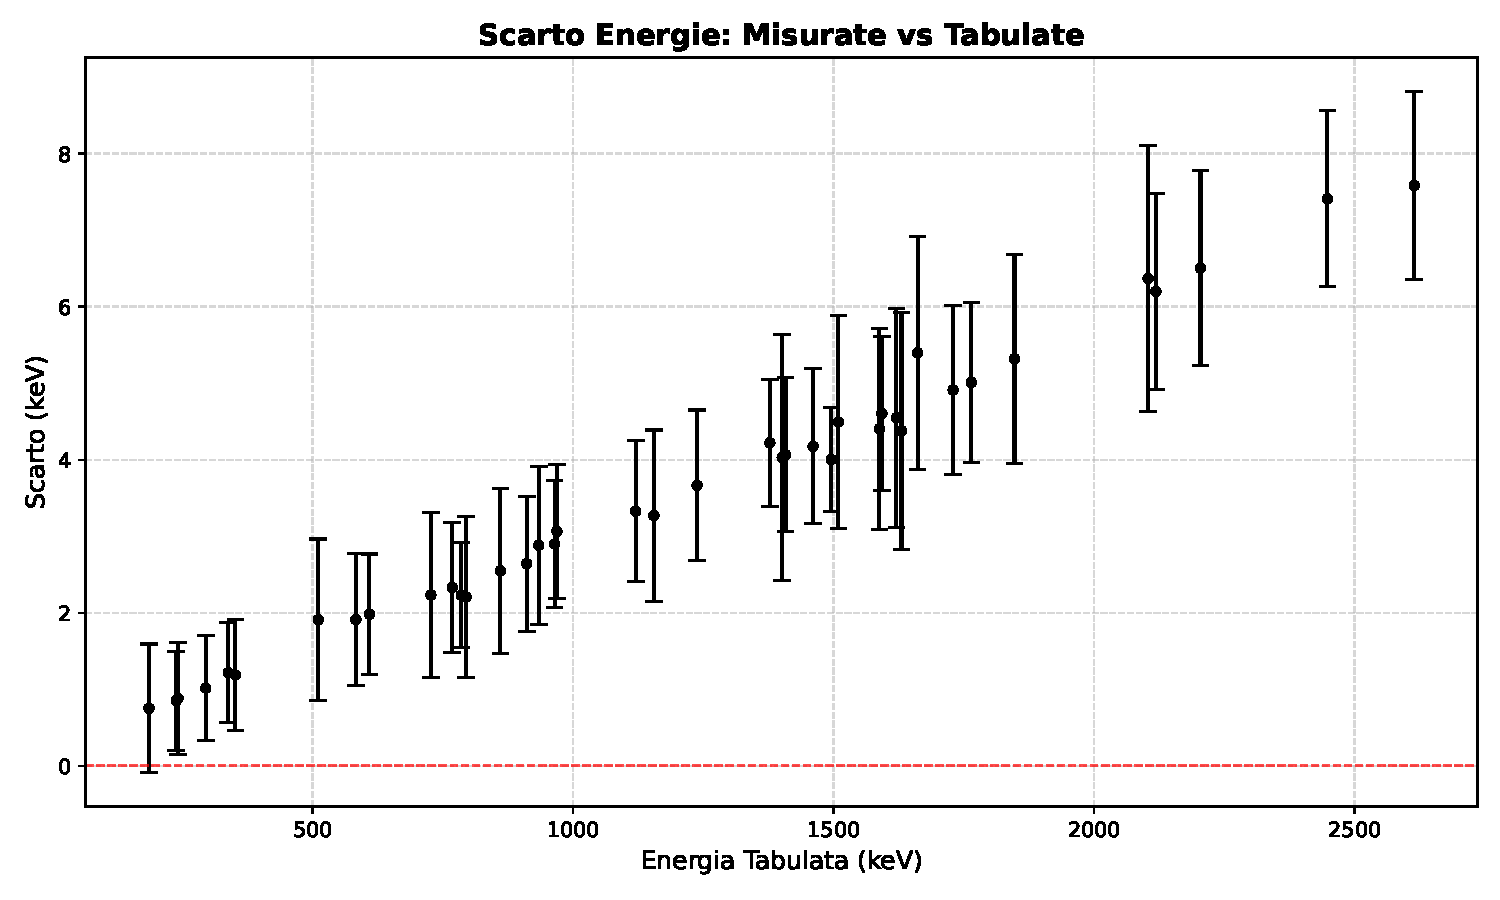
\includegraphics[width=14cm]{grafici/confronto_incognita.pdf}
            \end{figure}

            Il fatto che non vi sia compatibilità con lo zero (eccetto che per un picco, quello del radio-226) non è da considerare un fallimento sperimentale, anzi, che le energie misurate siano sovrastimate può indicare un surriscaldamento dell'apparato, dato che le misure per la sorgente incognita hanno un tempo molto più lungo:
            \begin{itemize}
                \item Errore sistematico costante per il surriscaldamento del convertitore ADC e aumento del parametro di calibrazione $\alpha$ (zero drift);
                \item Errore proporzionale all'energia per il surriscaldamento dell'amplificatore e aumento del parametro di calibrazione $\beta$ (gain drift).
            \end{itemize}
            Il coefficiente di correlazione lineare (calcolato dallo stesso script in python) pari a $r=0.995128$ è un'ottima conferma dell'andamento lineare del drift. Per cui, vale la pena indicare anche i parametri di fit lineare, corrispondenti alle modifiche, per il surriscaldamento, di zero drift e gain drift ai coefficienti della calibrazione in energia del rivelatore al germanio, rispettivamente, $\Delta\alpha$ e $\Delta\beta$:
            \begin{equation*}
                \boxed{\Delta\alpha=(0.167\pm0.062)\si{\kilo\electronvolt}\quad\Delta\beta=(2.824\pm0.045)\cdot10^{-3}\si{\kilo\electronvolt}/canali}
            \end{equation*}

        \subsection*{Il rumore elettronico}
            La figura \ref{fig:confronto_rumore} mostra il confronto tra la radice del parametro $a$ calcolato dal best fit caratteristico per le risoluzioni e la $FWHM$ del picco del pulser. Il loro confronto è rilevante perché entrambi quantificano il contributo del rumore elettronico al peggioramento della risoluzione. Nonostante siano dello stesso ordine di grandezza, non sono compatibili.
            \begin{figure}[h!]
                \centering
                \caption{Confronto FWHM pulser e $\sqrt{a}$}
                \label{fig:confronto_rumore}
                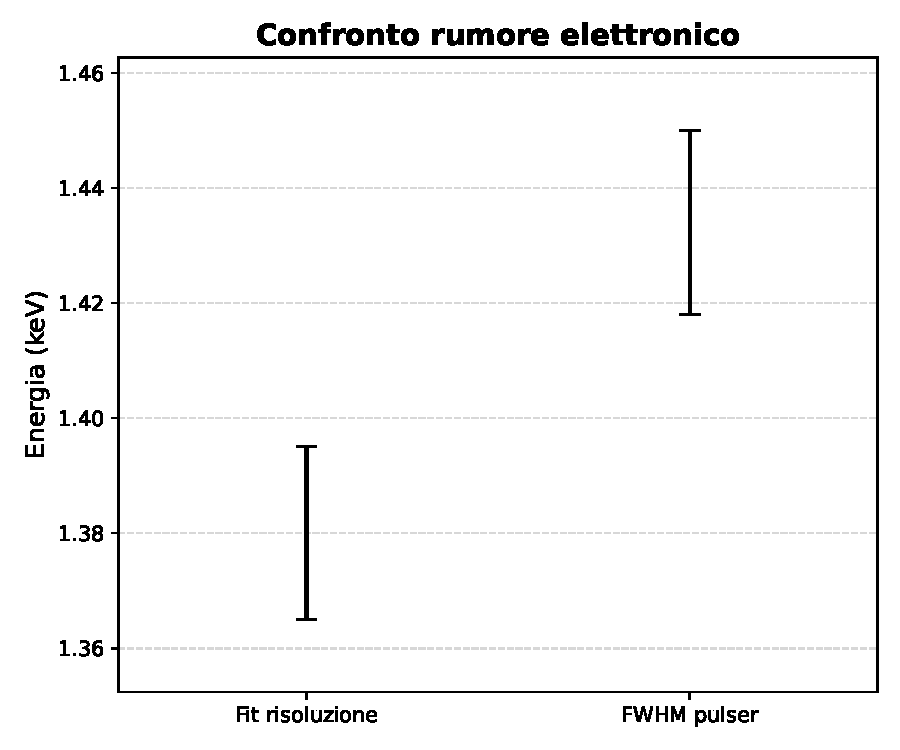
\includegraphics[width=8cm]{grafici/confronto_rumore.pdf}
            \end{figure}
        
        \subsection*{L'efficienza}
            Per quanto riguarda l'efficienza in percentuale dei picchi nell'HpGe, oltre alla verifica della formula parametrica caratteristica, è possibile confrontarne il valore per un picco del cobalto-60 ad alto rateo con quello dello standard NaI, dato che in quella misura la sorgente è stata posta appositamente a $\SI{25}{\centi\meter}$ dal rivelatore. A tal proposito, per il picco ad alta energia:
            \begin{align*}
                &\epsilon_{NaI}=0.2 \% \\
                &\epsilon_{mis}=0.01212 \%
            \end{align*}
            Cioè l'efficienza misurata è pari al $\boxed{6 \%}$ di quella dello standard, e questo indica il prezzo da pagare per avere una risoluzione eccellente: il germanio ha un numero atomico ben inferiore di quello efficace dello ioduro di sodio e assorbe meno i fotoni. Ad ogni modo, è un valore di efficienza relativa estremamente realistico, trattandosi di un rivelatore per scopi didattici.

        \subsection*{La coincidenza}
            Infine, la coincidenza dell'emissione di due gamma da parte del cobalto-60 può essere verificata con due confronti rispetto agli ultimi fit della tabella \ref{tab:fit_coincidenza}:
            \begin{itemize}
                \item I due picchi in canali per il rivelatore al fluoruro di bario non devono sovrapporsi entro la loro $FWHM$;
                \item I centroidi dei picchi in canali a bassa energia nel rivelatore BaF, misurati nello spettro totale e in quello acquisito in coincidenza (con soglia sull'HpGe), devono risultare statisticamente compatibili.
            \end{itemize}

            La figura \ref{fig:confronto_coincidenza} mostra suddetto confronto, che verifica con successo entrambe le condizioni.

            \begin{figure}[h!]
                \centering
                \caption{Confronto per coincidenza BaF}
                \label{fig:confronto_coincidenza}
                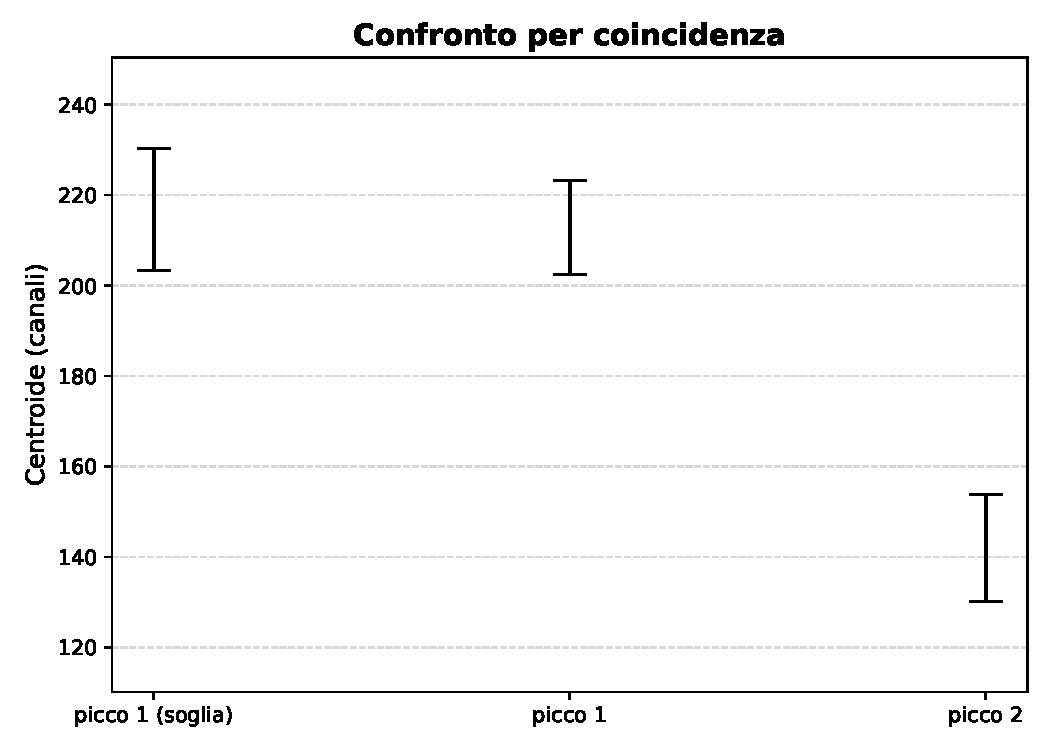
\includegraphics[width=8cm]{grafici/confronto_coincidenza.pdf}
            \end{figure}

            Infine, vale la pena osservare che la risoluzione percentuale dei picchi nel BaF è di uno o due ordini di grandezza superiore di quella dei picchi dell'HpGe: questa è la conferma che pur di avere una risposta temporale migliore, nel rivelatore a scintillazione si rinuncia a una buona distinzione dei picchi.

        \newpage
        \section*{Bibliografia e sitografia}
        \begin{itemize}
            \item Slides fornite dal docente;
            \item Radiation Detection and Measurement, Glenn F. Knoll;
            \item https://github.com/valerio-capuano/spettroscopia-gamma (con tutti i codici ROOT e python).
        \end{itemize}
        
        
            
\end{document}
